% Options for packages loaded elsewhere
\PassOptionsToPackage{unicode}{hyperref}
\PassOptionsToPackage{hyphens}{url}
\documentclass[
  12pt,
]{article}
\usepackage{xcolor}
\usepackage[margin=1in]{geometry}
\usepackage{amsmath,amssymb}
\setcounter{secnumdepth}{5}
\usepackage{iftex}
\ifPDFTeX
  \usepackage[T1]{fontenc}
  \usepackage[utf8]{inputenc}
  \usepackage{textcomp} % provide euro and other symbols
\else % if luatex or xetex
  \usepackage{unicode-math} % this also loads fontspec
  \defaultfontfeatures{Scale=MatchLowercase}
  \defaultfontfeatures[\rmfamily]{Ligatures=TeX,Scale=1}
\fi
\usepackage{lmodern}
\ifPDFTeX\else
  % xetex/luatex font selection
\fi
% Use upquote if available, for straight quotes in verbatim environments
\IfFileExists{upquote.sty}{\usepackage{upquote}}{}
\IfFileExists{microtype.sty}{% use microtype if available
  \usepackage[]{microtype}
  \UseMicrotypeSet[protrusion]{basicmath} % disable protrusion for tt fonts
}{}
\makeatletter
\@ifundefined{KOMAClassName}{% if non-KOMA class
  \IfFileExists{parskip.sty}{%
    \usepackage{parskip}
  }{% else
    \setlength{\parindent}{0pt}
    \setlength{\parskip}{6pt plus 2pt minus 1pt}}
}{% if KOMA class
  \KOMAoptions{parskip=half}}
\makeatother
\usepackage{graphicx}
\makeatletter
\newsavebox\pandoc@box
\newcommand*\pandocbounded[1]{% scales image to fit in text height/width
  \sbox\pandoc@box{#1}%
  \Gscale@div\@tempa{\textheight}{\dimexpr\ht\pandoc@box+\dp\pandoc@box\relax}%
  \Gscale@div\@tempb{\linewidth}{\wd\pandoc@box}%
  \ifdim\@tempb\p@<\@tempa\p@\let\@tempa\@tempb\fi% select the smaller of both
  \ifdim\@tempa\p@<\p@\scalebox{\@tempa}{\usebox\pandoc@box}%
  \else\usebox{\pandoc@box}%
  \fi%
}
% Set default figure placement to htbp
\def\fps@figure{htbp}
\makeatother
\setlength{\emergencystretch}{3em} % prevent overfull lines
\providecommand{\tightlist}{%
  \setlength{\itemsep}{0pt}\setlength{\parskip}{0pt}}
\usepackage[round]{natbib}
\bibliographystyle{plainnat}
\usepackage{url}
%\usepackage{xurl}
\usepackage{setspace}
\singlespacing
%\onehalfspacing
%\doublespacing
\usepackage{lineno}
%\linenumbers
\usepackage[belowskip=0pt,aboveskip=0pt]{caption}
\usepackage{relsize}
\usepackage{float}
\usepackage{lscape}
\usepackage{longtable}
\usepackage{amsmath,rotating}
\usepackage[scanall]{psfrag}
\usepackage{bm}
\usepackage{caption,graphics}
\usepackage{graphicx}
\usepackage{sectsty}
\usepackage{color}
\usepackage{fancyhdr}
\usepackage{xspace}
\usepackage{textcomp}
\usepackage{upgreek}
% \usepackage{booktabs}
% \usepackage{threeparttable}
\renewcommand\figurename{Fig.}
\captionsetup{labelsep=period, singlelinecheck=false}
\newcommand{\changesize}[1]{\fontsize{#1pt}{#1pt}\selectfont}
\renewcommand{\arraystretch}{1.5}
%\renewcommand\theadfont{}

\newcommand{\Fmsy}{\ensuremath{F_{\text{MSY}}}\xspace}
\newcommand{\Fspr}[1]{\ensuremath{F_{\text{{#1}\%}}}\xspace}
\usepackage{booktabs}
\usepackage{longtable}
\usepackage{array}
\usepackage{multirow}
\usepackage{wrapfig}
\usepackage{float}
\usepackage{colortbl}
\usepackage{pdflscape}
\usepackage{tabu}
\usepackage{threeparttable}
\usepackage{threeparttablex}
\usepackage[normalem]{ulem}
\usepackage{makecell}
\usepackage{xcolor}
\usepackage{bookmark}
\IfFileExists{xurl.sty}{\usepackage{xurl}}{} % add URL line breaks if available
\urlstyle{same}
\hypersetup{
  hidelinks,
  pdfcreator={LaTeX via pandoc}}

\title{Factors affecting inferences on natural mortality and associated
environmental effects in state-space age-structured assessment models:\\
Supplementary Materials}
\author{}
\date{\vspace{-2.5em}}

\begin{document}
\maketitle

Timothy J. Miller: ORCID ID 0000-0003-1411-1206; corresponding author:
\href{mailto:timothy.j.miller@noaa.gov}{\nolinkurl{timothy.j.miller@noaa.gov}};
Northeast Fisheries Science Center, Woods Hole Laboratory, 166 Water
Street, Woods Hole, MA 02543 USA\\
\strut \\
Gregory L. Britten: ORCID ID 0000-0003-1391-9086; Biology Department,
Woods Hole Oceanographic Institution, 266 Woods Hole Rd. Woods Hole, MA,
USA\\
\strut \\
Elizabeth N. Brooks: ORCID ID 0000-0002-9142-4372; Northeast Fisheries
Science Center, Woods Hole Laboratory, 166 Water Street, Woods Hole, MA
02543 USA\\
\strut \\
Gavin Fay: ORCID ID 0000-0003-0425-9952; Department of Fisheries
Oceanography, School for Marine Science and Technology, University of
Massachusetts Dartmouth, 836 S Rodney French Boulevard, New Bedford, MA
02740, USA\\
\strut \\
Alexander C. Hansell: ORCID ID 0000-0001-7827-1749; Northeast Fisheries
Science Center, Woods Hole Laboratory, 166 Water Street, Woods Hole, MA
02543 USA\\
\strut \\
Christopher M. Legault: ORCID ID 0000-0002-0328-1376; Northeast
Fisheries Science Center, Woods Hole Laboratory, 166 Water Street, Woods
Hole, MA 02543 USA\\
\strut \\
Brandon Muffley: ORCID ID 0009-0005-8681-0489; Mid-Atlantic Fishery
Management Council, 800 North State Street, Suite 201, Dover, DE 19901
USA\\
\strut \\
John Wiedenmann: ORCID ID 0000-0001-7622-9053; Department of Ecology,
Evolution, and Natural Resources, Rutgers University, 14 College Farm Rd
W, New Brunswick, NJ 08901 USA\\

\pagebreak

\setcounter{figure}{0}
\renewcommand\thefigure{S\arabic{figure}}

\setcounter{table}{0}
\renewcommand\thetable{S\arabic{table}}

\pagebreak

\pagebreak

\section*{Referenced Figures}\label{referenced-figures}
\addcontentsline{toc}{section}{Referenced Figures}

\begin{landscape}
\begin{figure}
\begin{center}
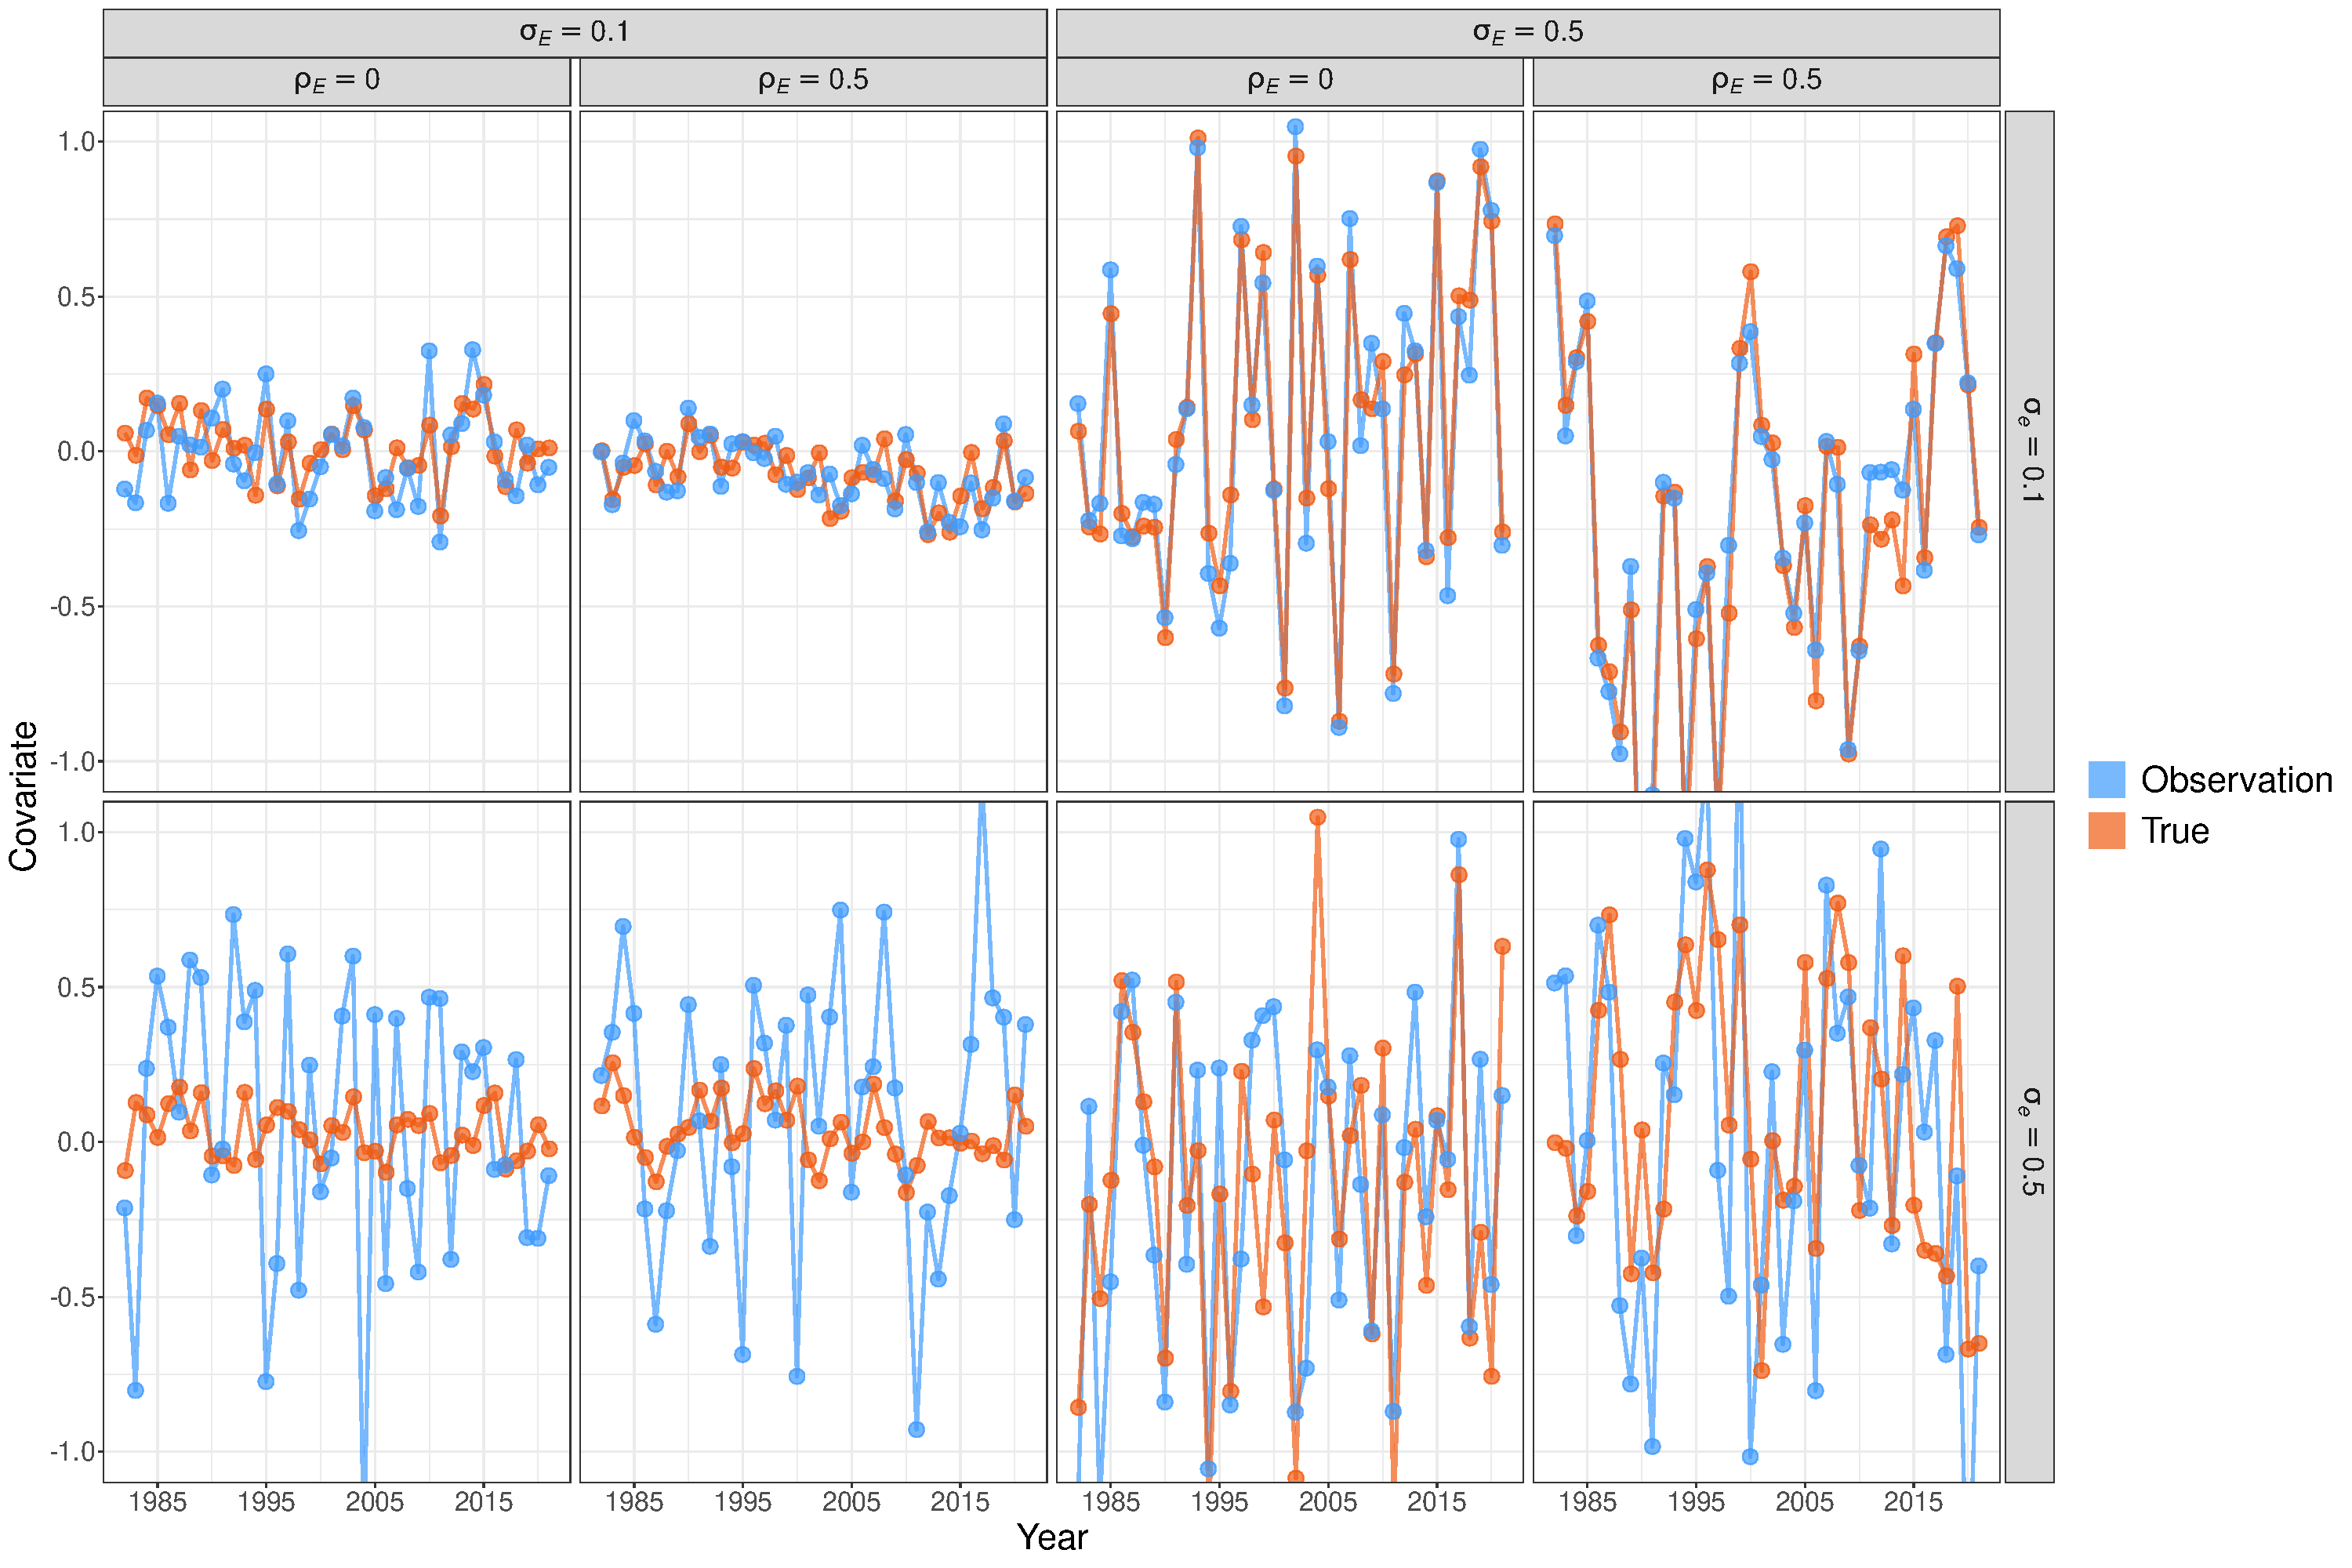
\includegraphics[height = \textheight]{Ecov_true_obs_example}
\end{center}
\caption{Example simulations of environmental covariate latent processes and observations with different levels of observation error, and different assumptions about variability of the latent process.}\label{om_ecov_example}
\end{figure}
\end{landscape}

\begin{figure}
\begin{center}
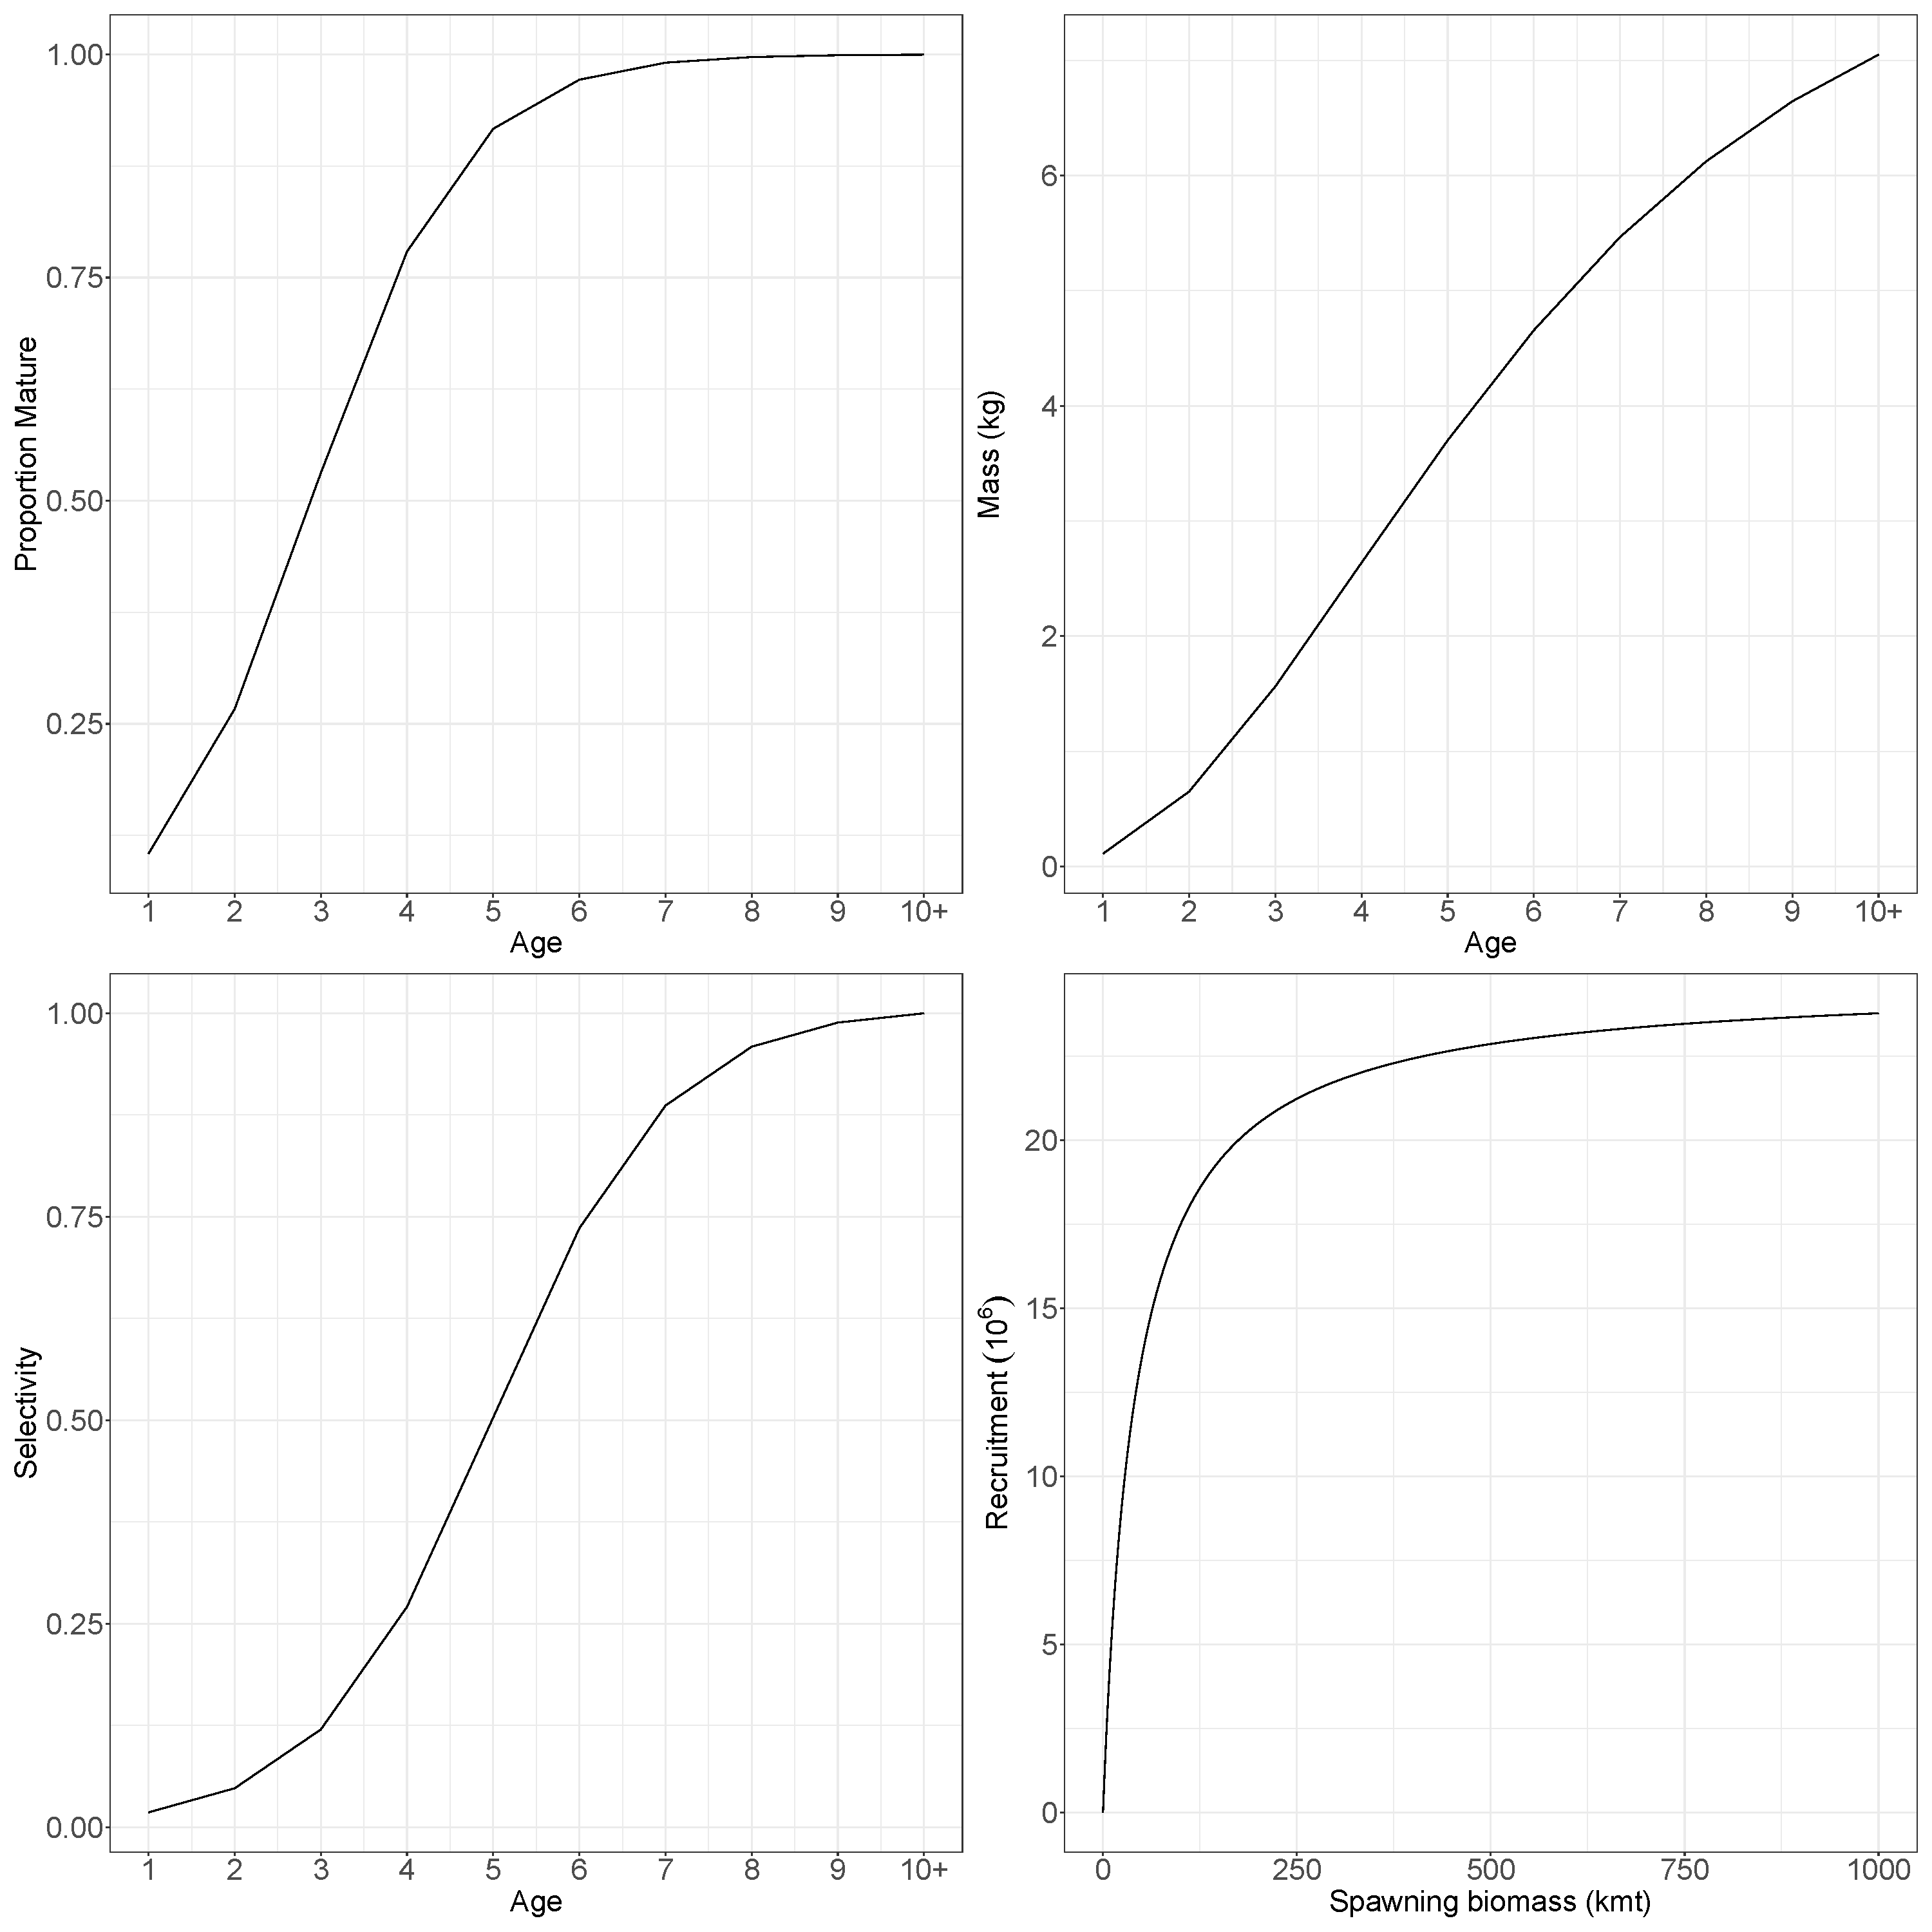
\includegraphics[width = \textwidth]{om_input_plots_figure}
\end{center}
\caption{The proportion mature at age, weight at age, fleet and index selectivity at age, and Beverton-Holt stock-recruit relationship assumed for the population in all operating models. For operating models with random effects on fleet selectivity, this represents the selectivity at the mean of the random effects.}\label{om_inputs_fig}
\end{figure}

\begin{landscape}
\begin{figure}
\begin{center}
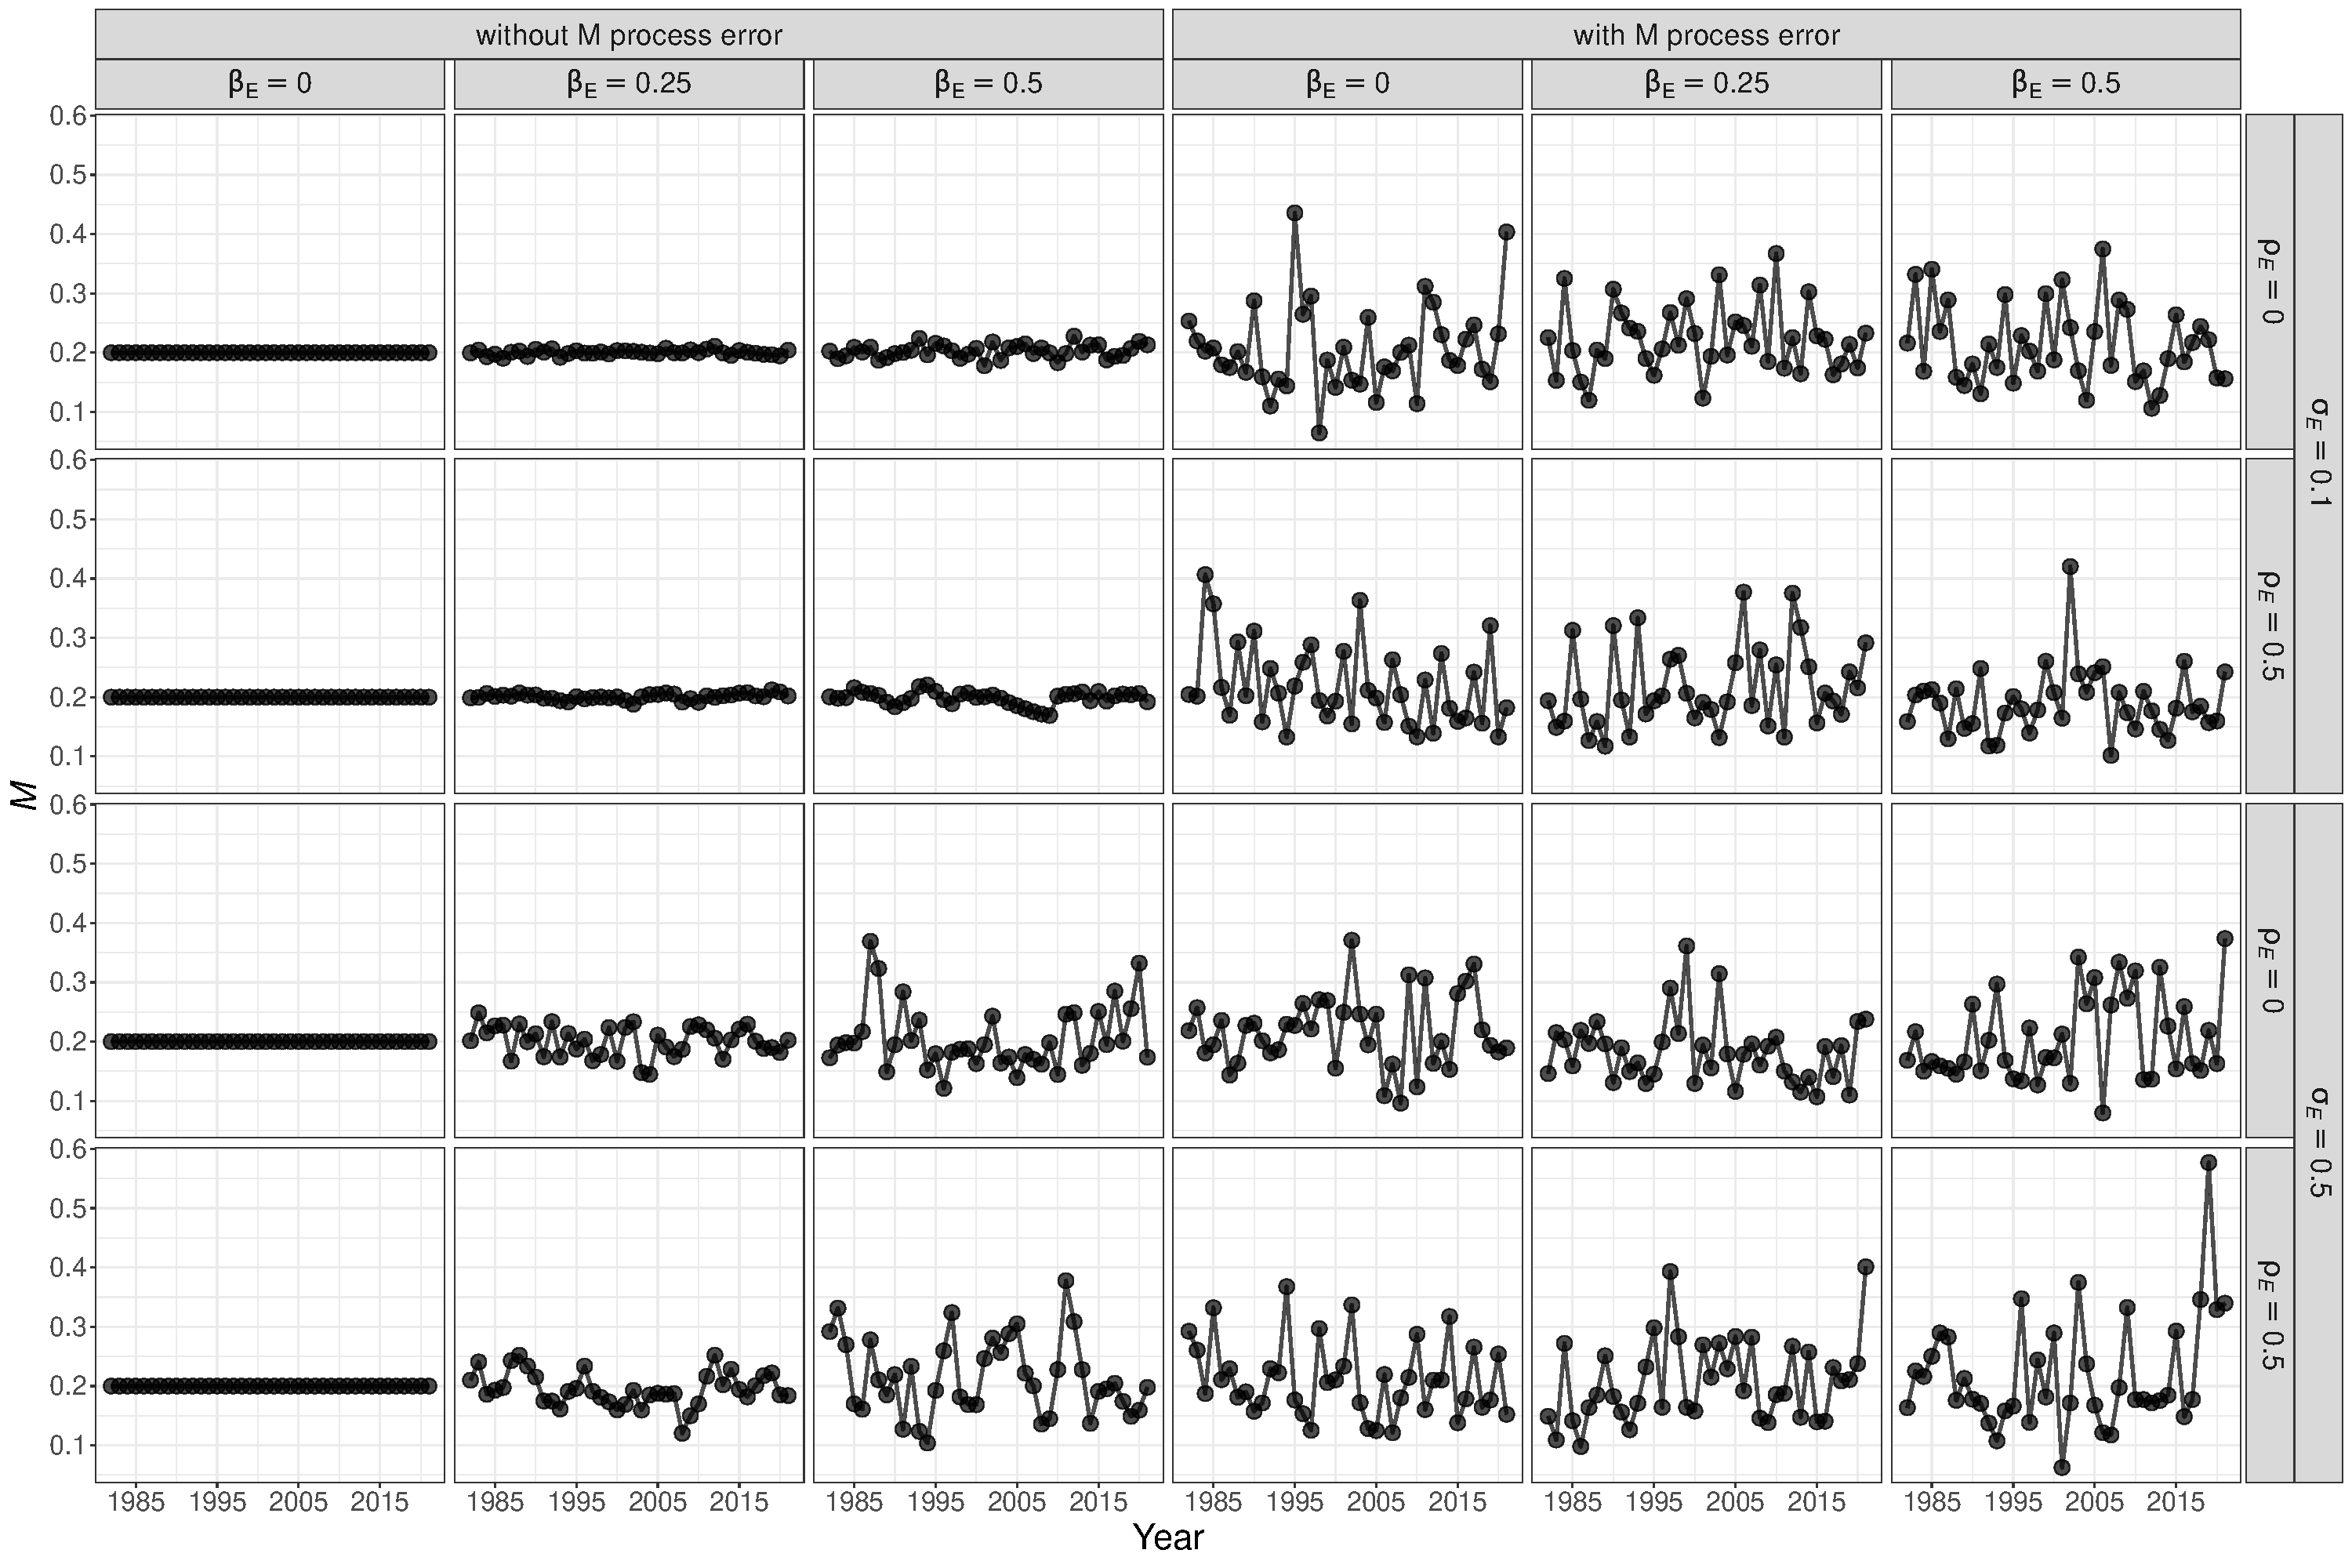
\includegraphics[height = \textheight]{M_example}
\end{center}
\caption{Example simulations of annual $M$ that may be a function of a temporally varying environmental covariate and autoregressive random effects. The marginal standard devation of random effects is $\sigma_M = 0.3$.}\label{M_example}
\end{figure}
\end{landscape}

\begin{landscape}
\begin{figure}
\begin{center}
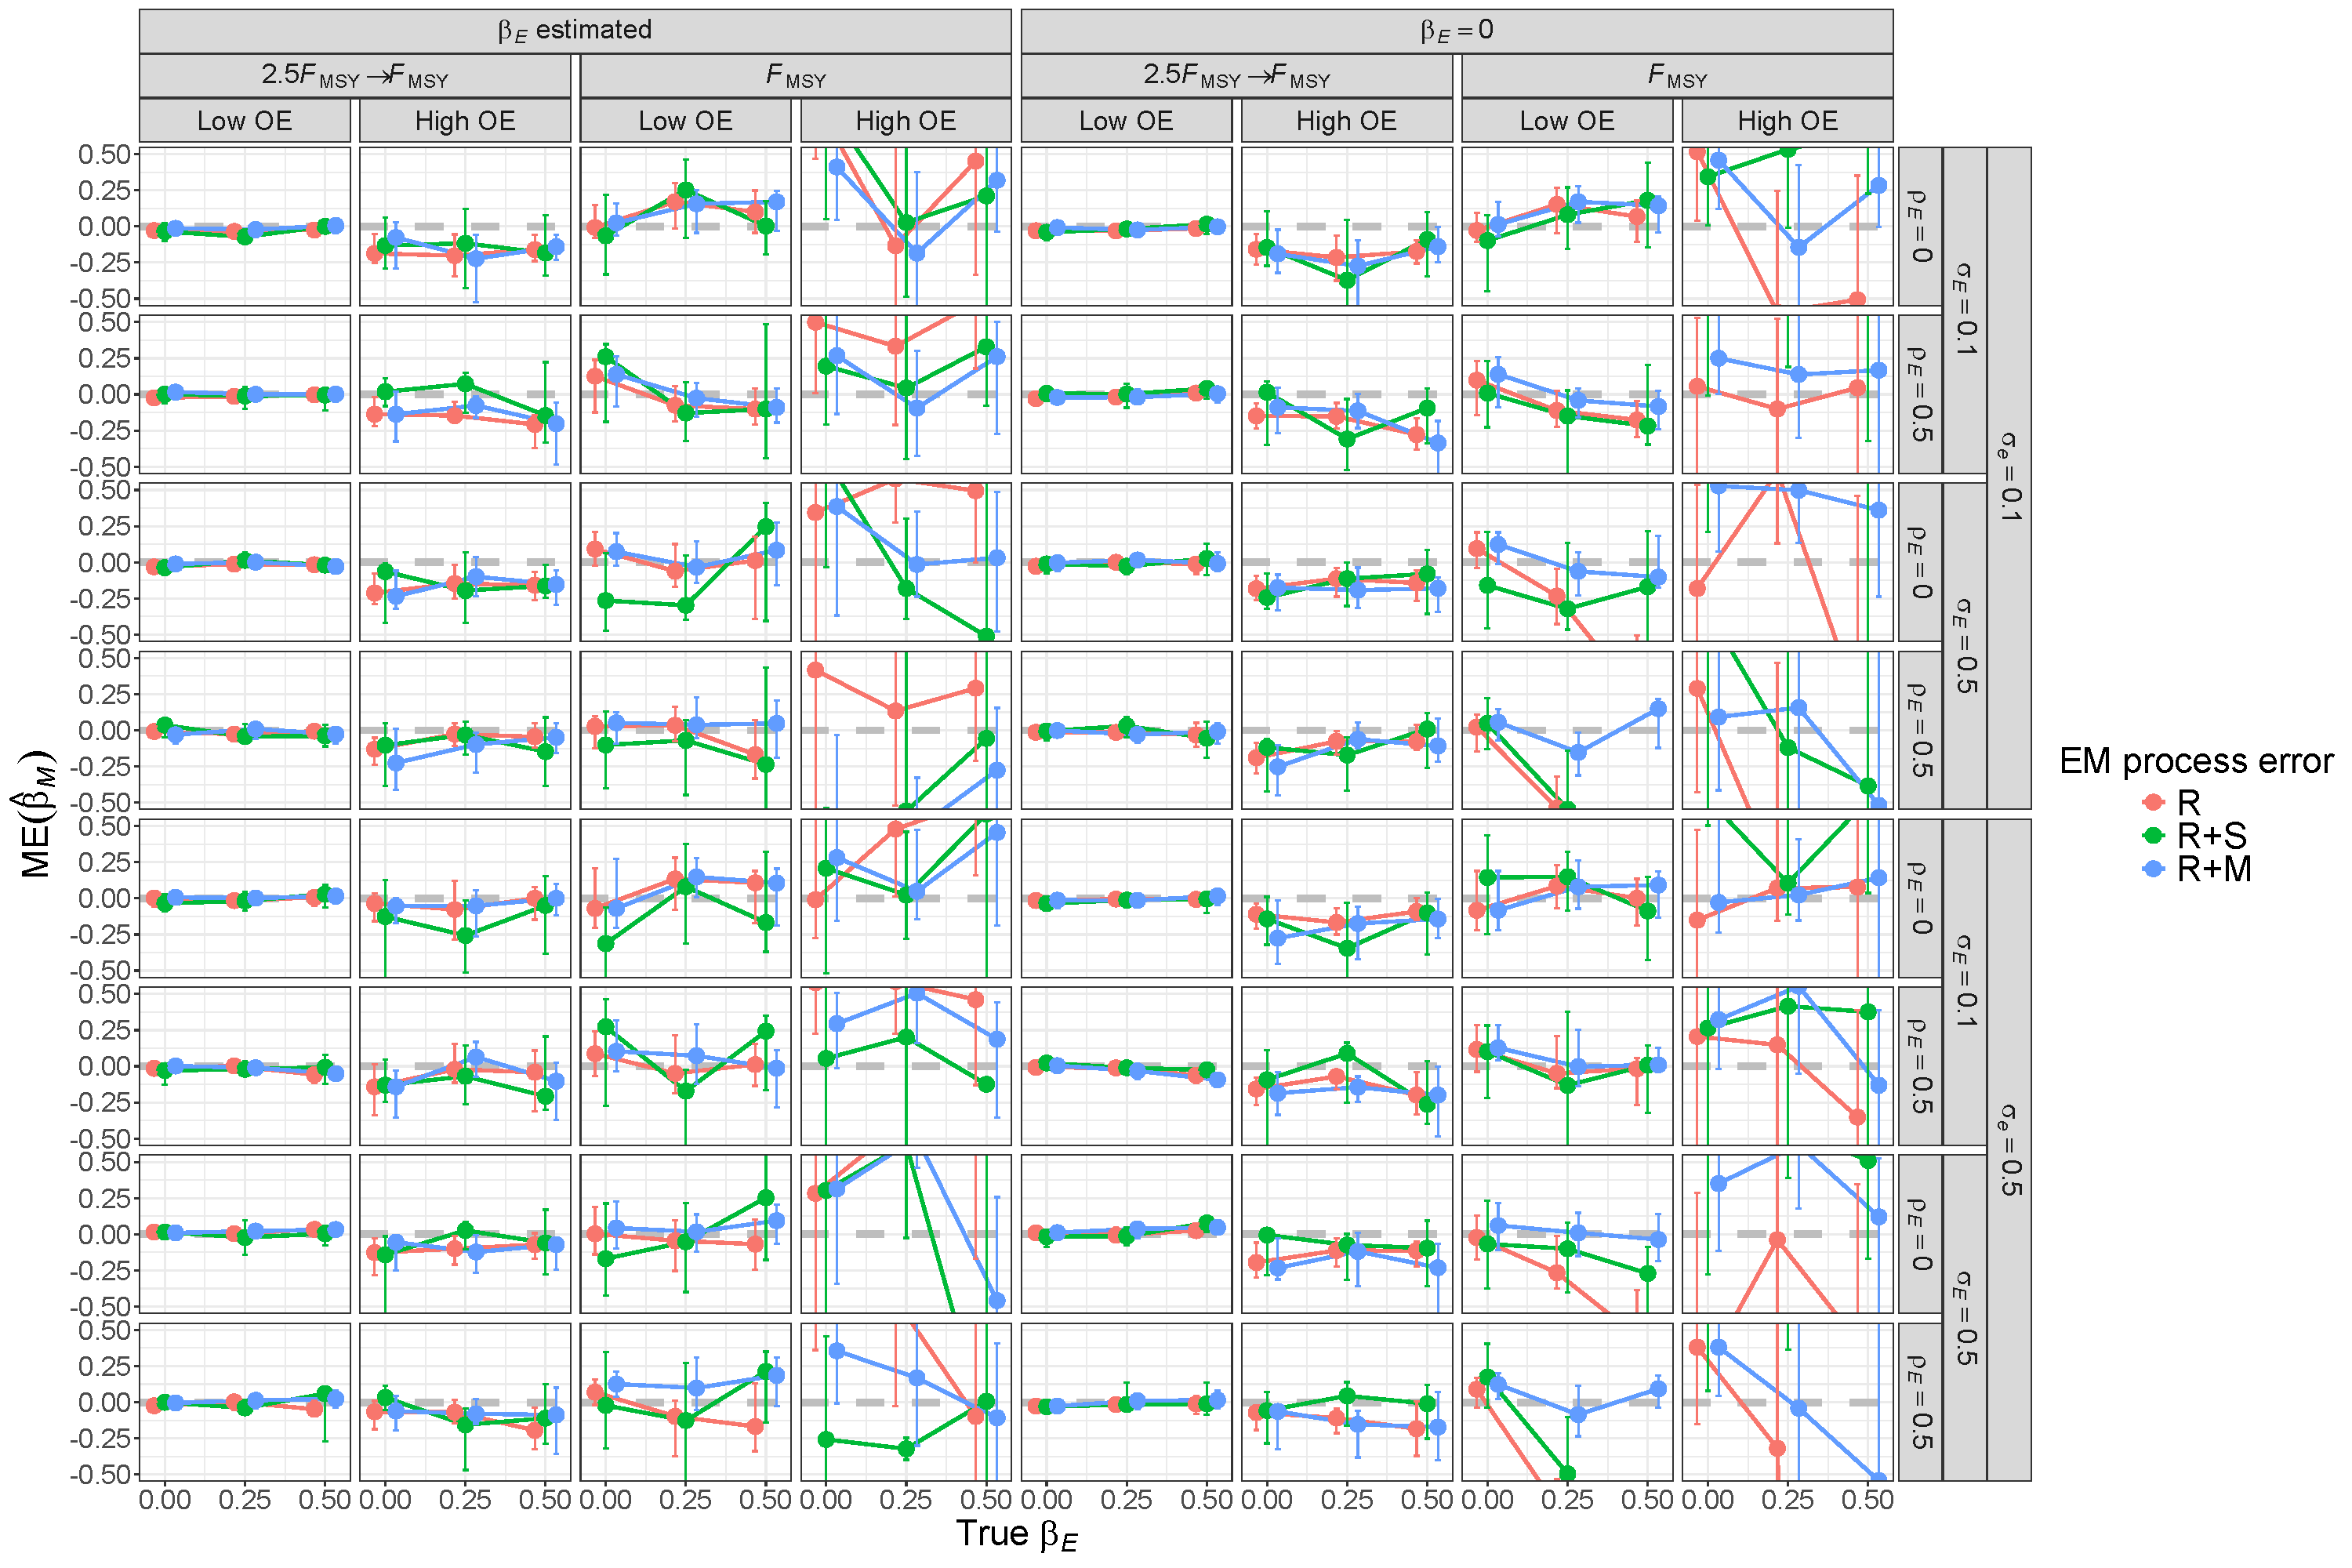
\includegraphics[height = \textheight]{beta_M_bias_Rom}
\end{center}
\caption{For R operating models, median error (ME) of estimates of $\beta_M$ from fitting estimating models with alternative process error assumptions and treatment of covariate effect ($\beta_E = 0$ or estimated). Vertical lines represent 95\% confidence intervals.}\label{beta_M_bias_Rom}
\end{figure}
\end{landscape}

\begin{landscape}
\begin{figure}
\begin{center}
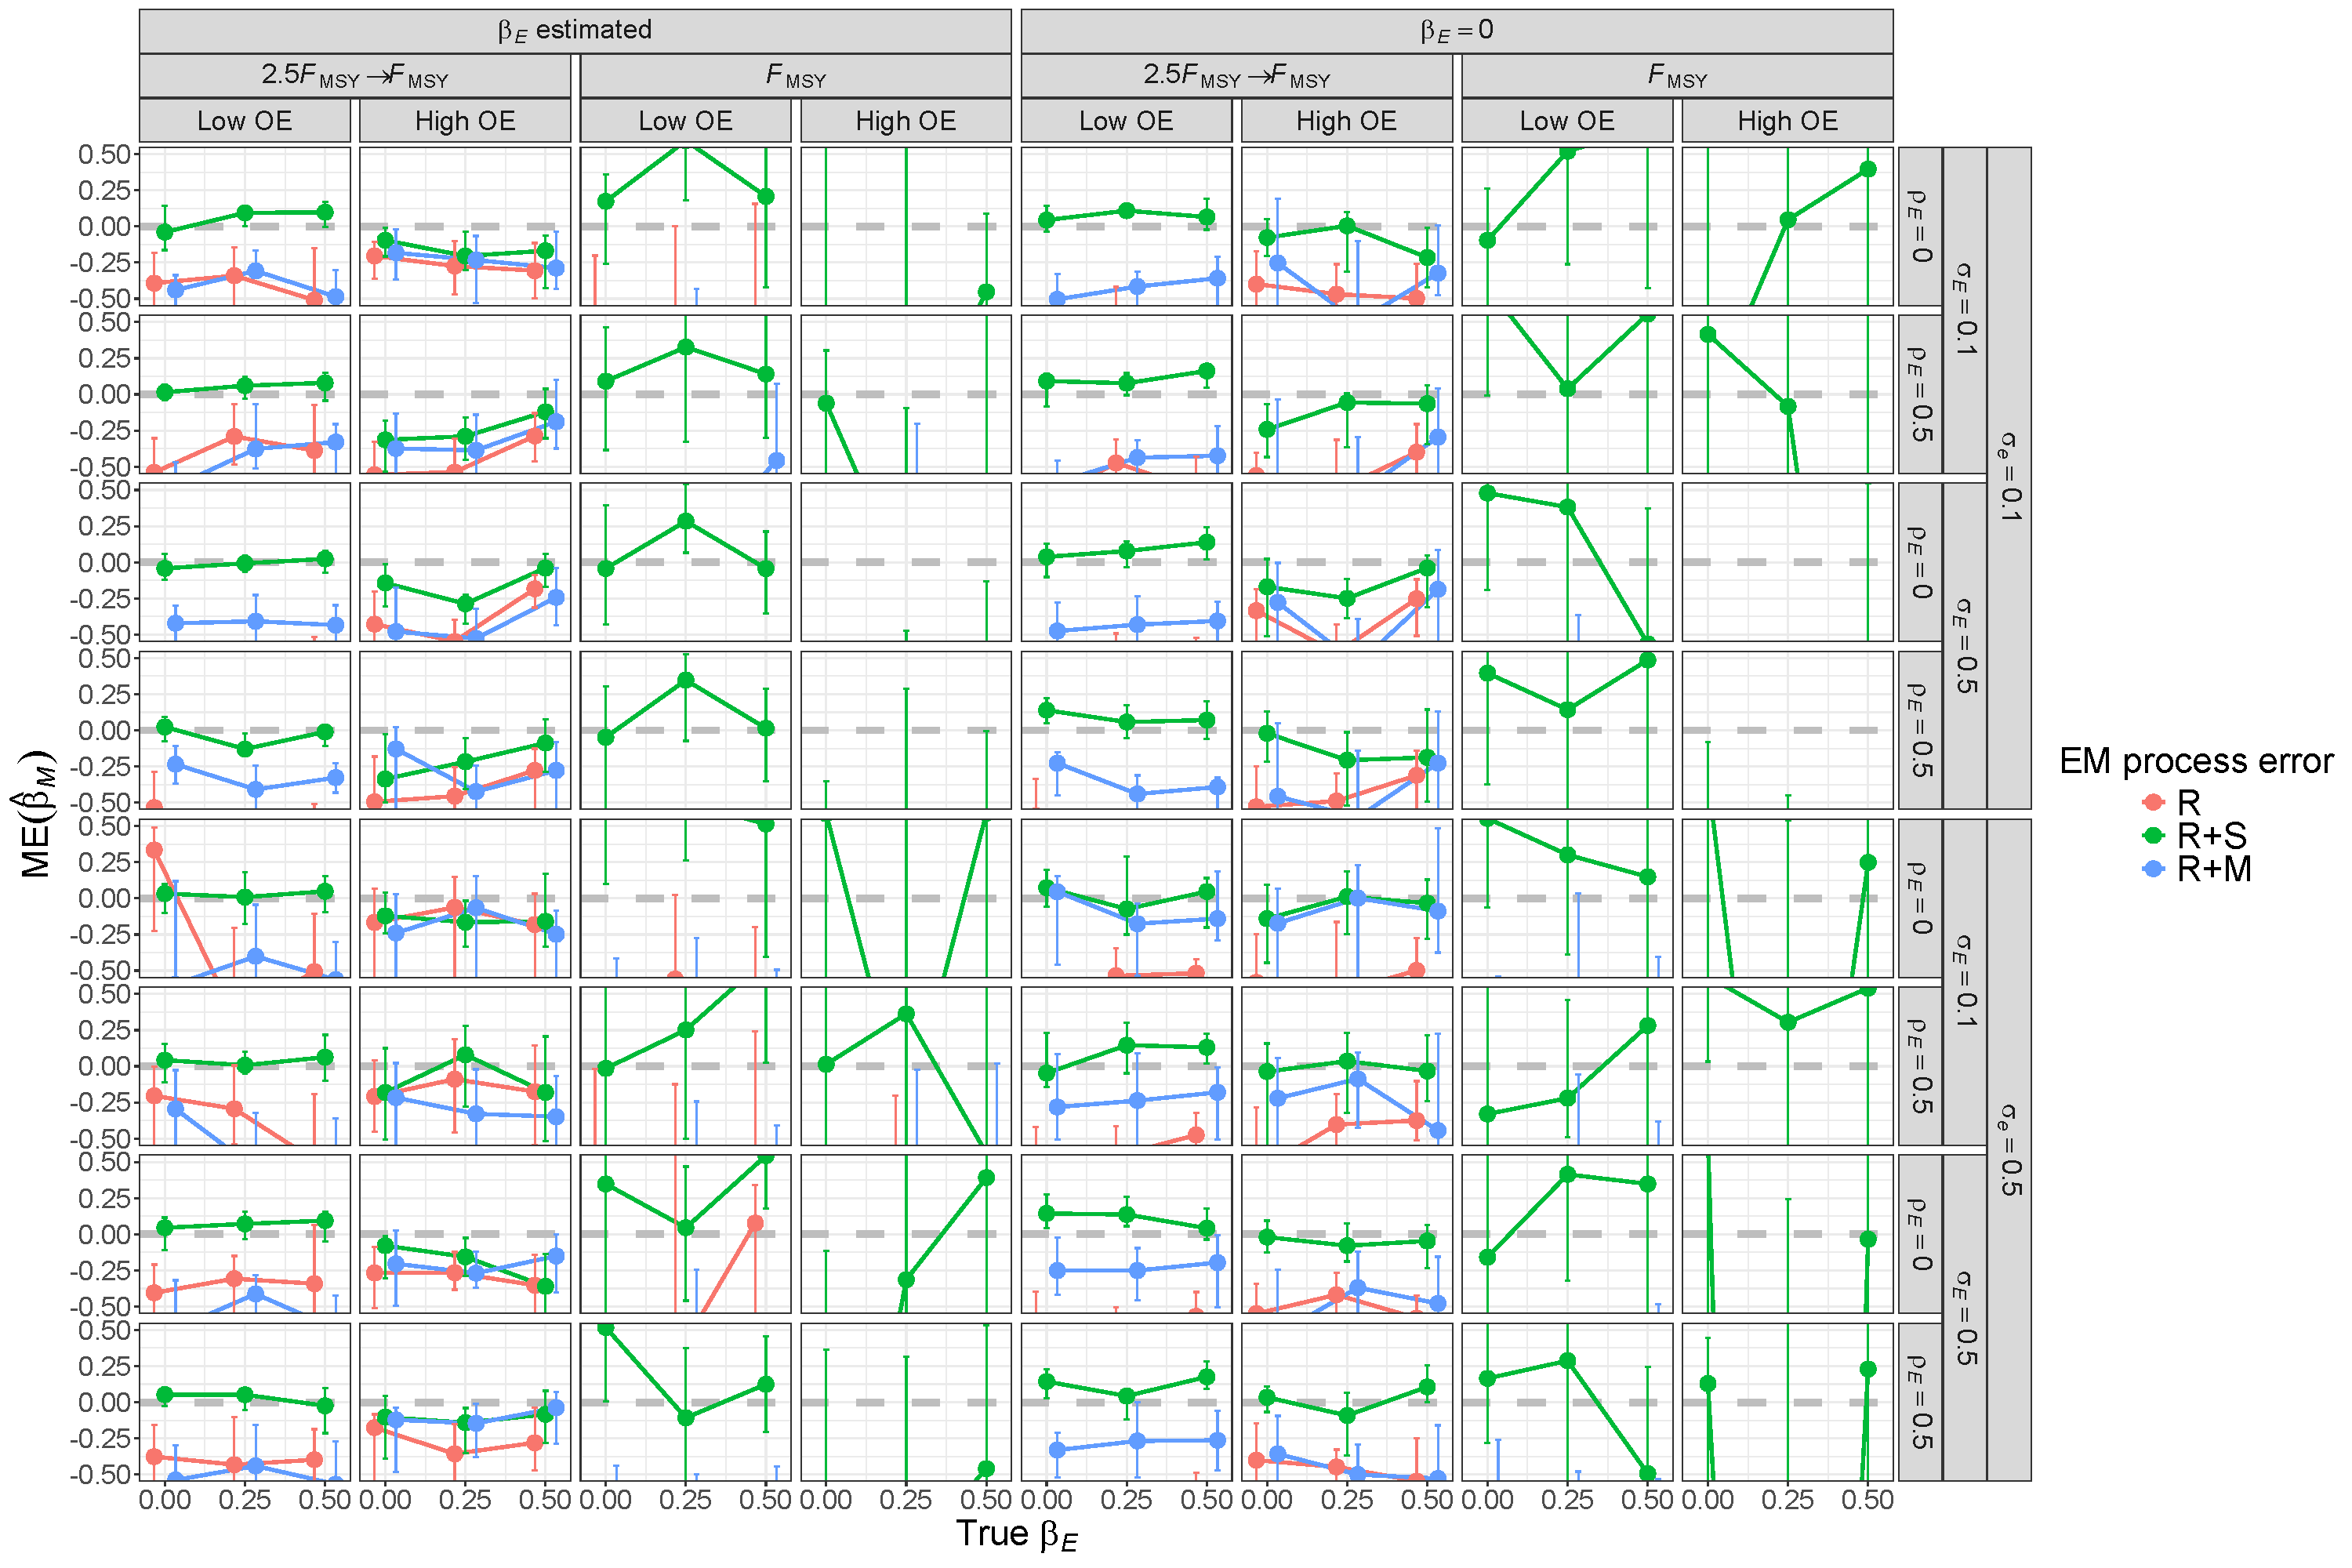
\includegraphics[height = \textheight]{beta_M_bias_RSom}
\end{center}
\caption{For R+S operating models, median error (ME) of estimates of $\beta_M$ from fitting estimating models with alternative process error assumptions and treatment of covariate effect ($\beta_E = 0$ or estimated). Vertical lines represent 95\% confidence intervals.}\label{beta_M_bias_RSom}
\end{figure}
\end{landscape}

\begin{landscape}
\begin{figure}
\begin{center}
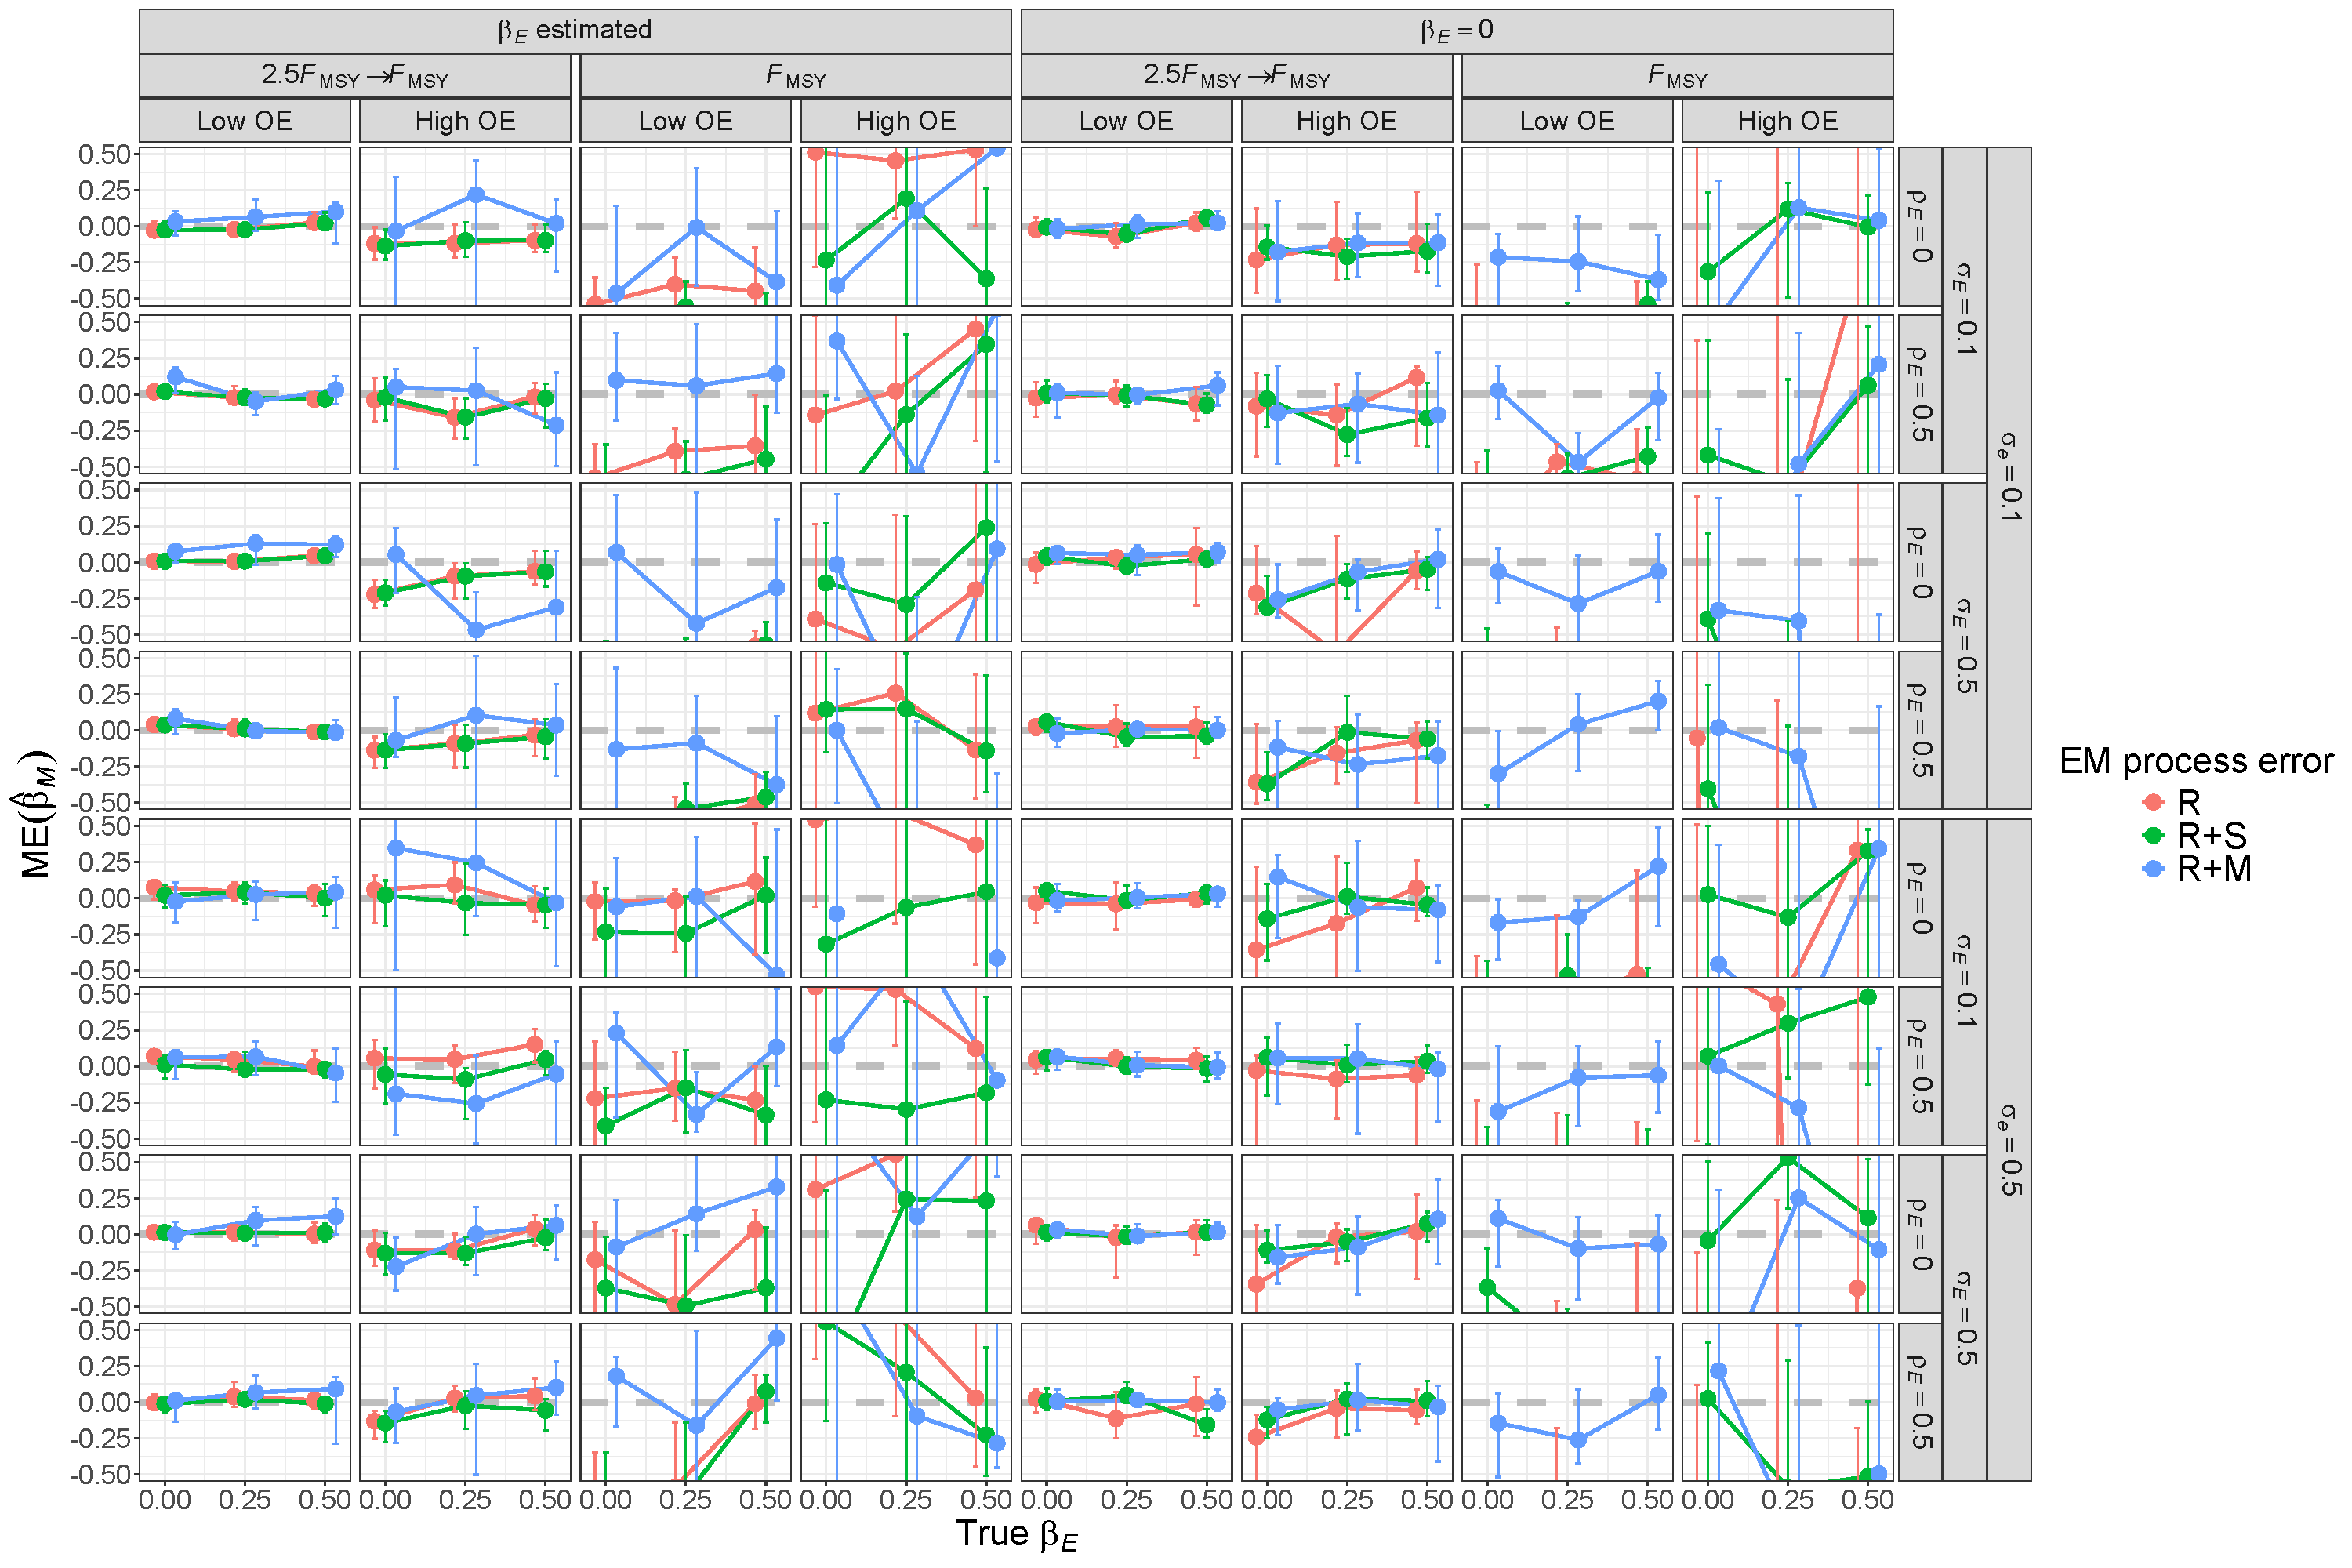
\includegraphics[height = \textheight]{beta_M_bias_RMom}
\end{center}
\caption{For R+M operating models, median error (ME) of estimates of $\beta_M$ from fitting estimating models with alternative process error assumptions and treatment of covariate effect ($\beta_E = 0$ or estimated). Vertical lines represent 95\% confidence intervals.}\label{beta_M_bias_RMom}
\end{figure}
\end{landscape}

\begin{landscape}
\begin{figure}
\begin{center}
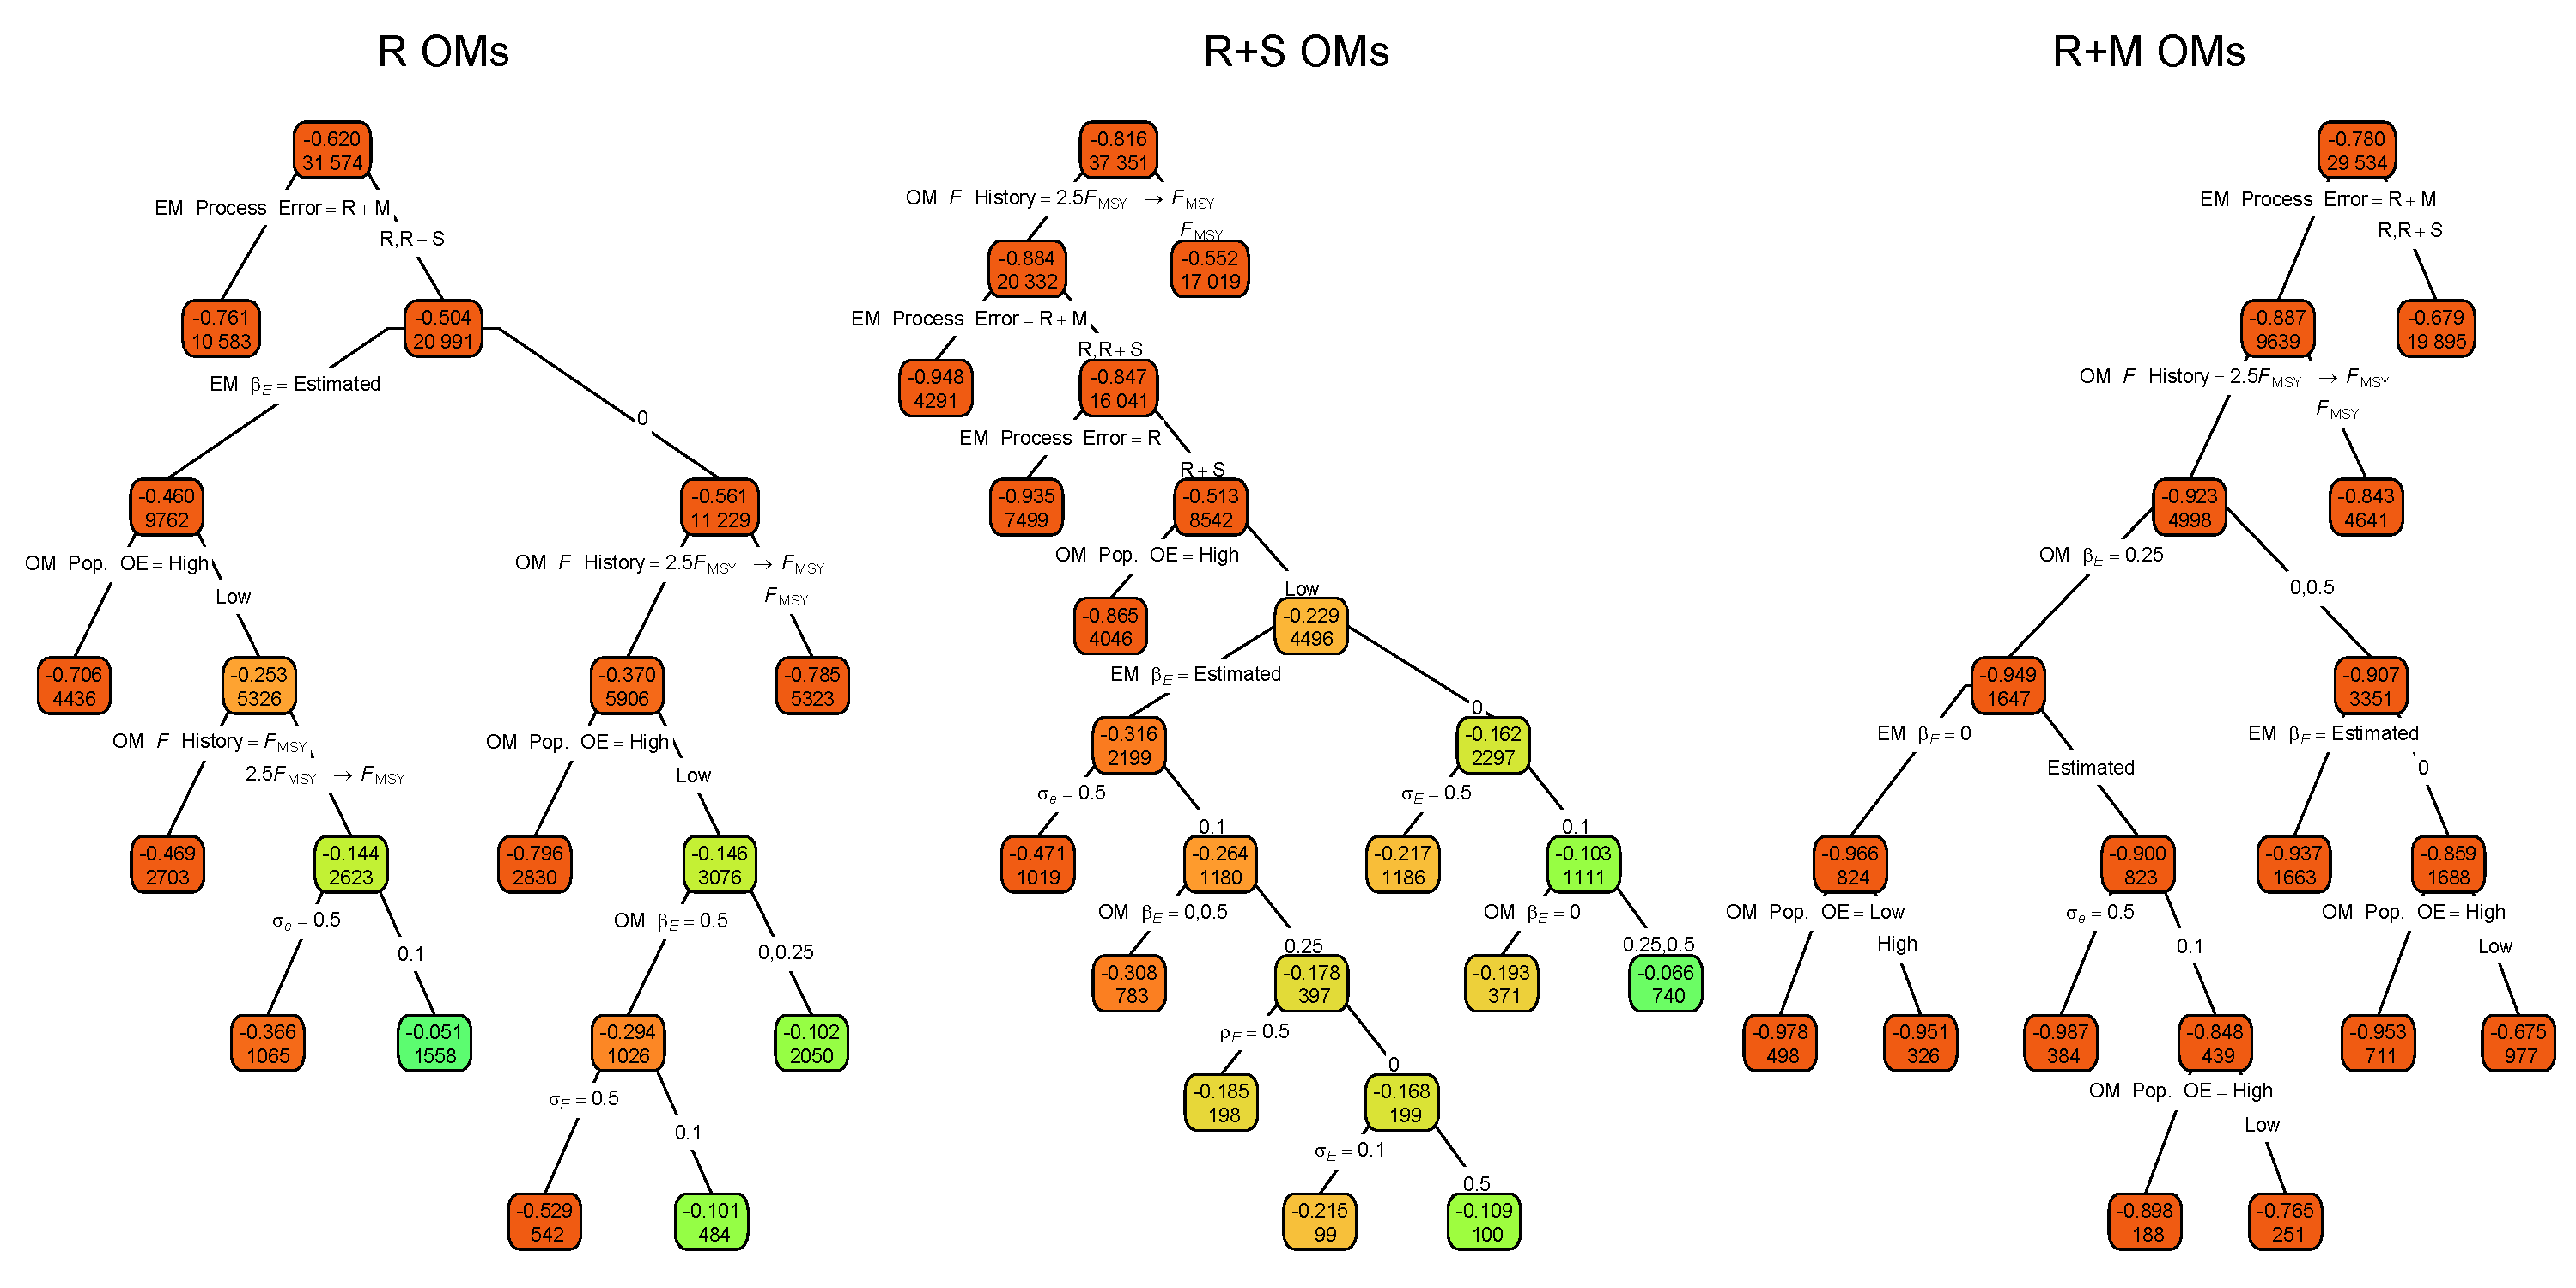
\includegraphics[width = 1.4\textwidth]{median_M_SE_bias_regtree_plots}
\end{center}
\caption{Regression trees for errors of the Hessian-based standard error estimates for median $M$ parameter ($\widehat {\text{SE}}\left(\widehat \beta_M\right)$). Each node shows the median error for the corresponding subset. Lower or higher absolute median absolute errors of the process error assumption are indicated by more green or red polygons, respectively. See Figure 1 caption and Table \ref{factor_table} for further details.}\label{med_M_SE_bias_regtree}
\end{figure}
\end{landscape}

\begin{landscape}
\begin{figure}
\begin{center}
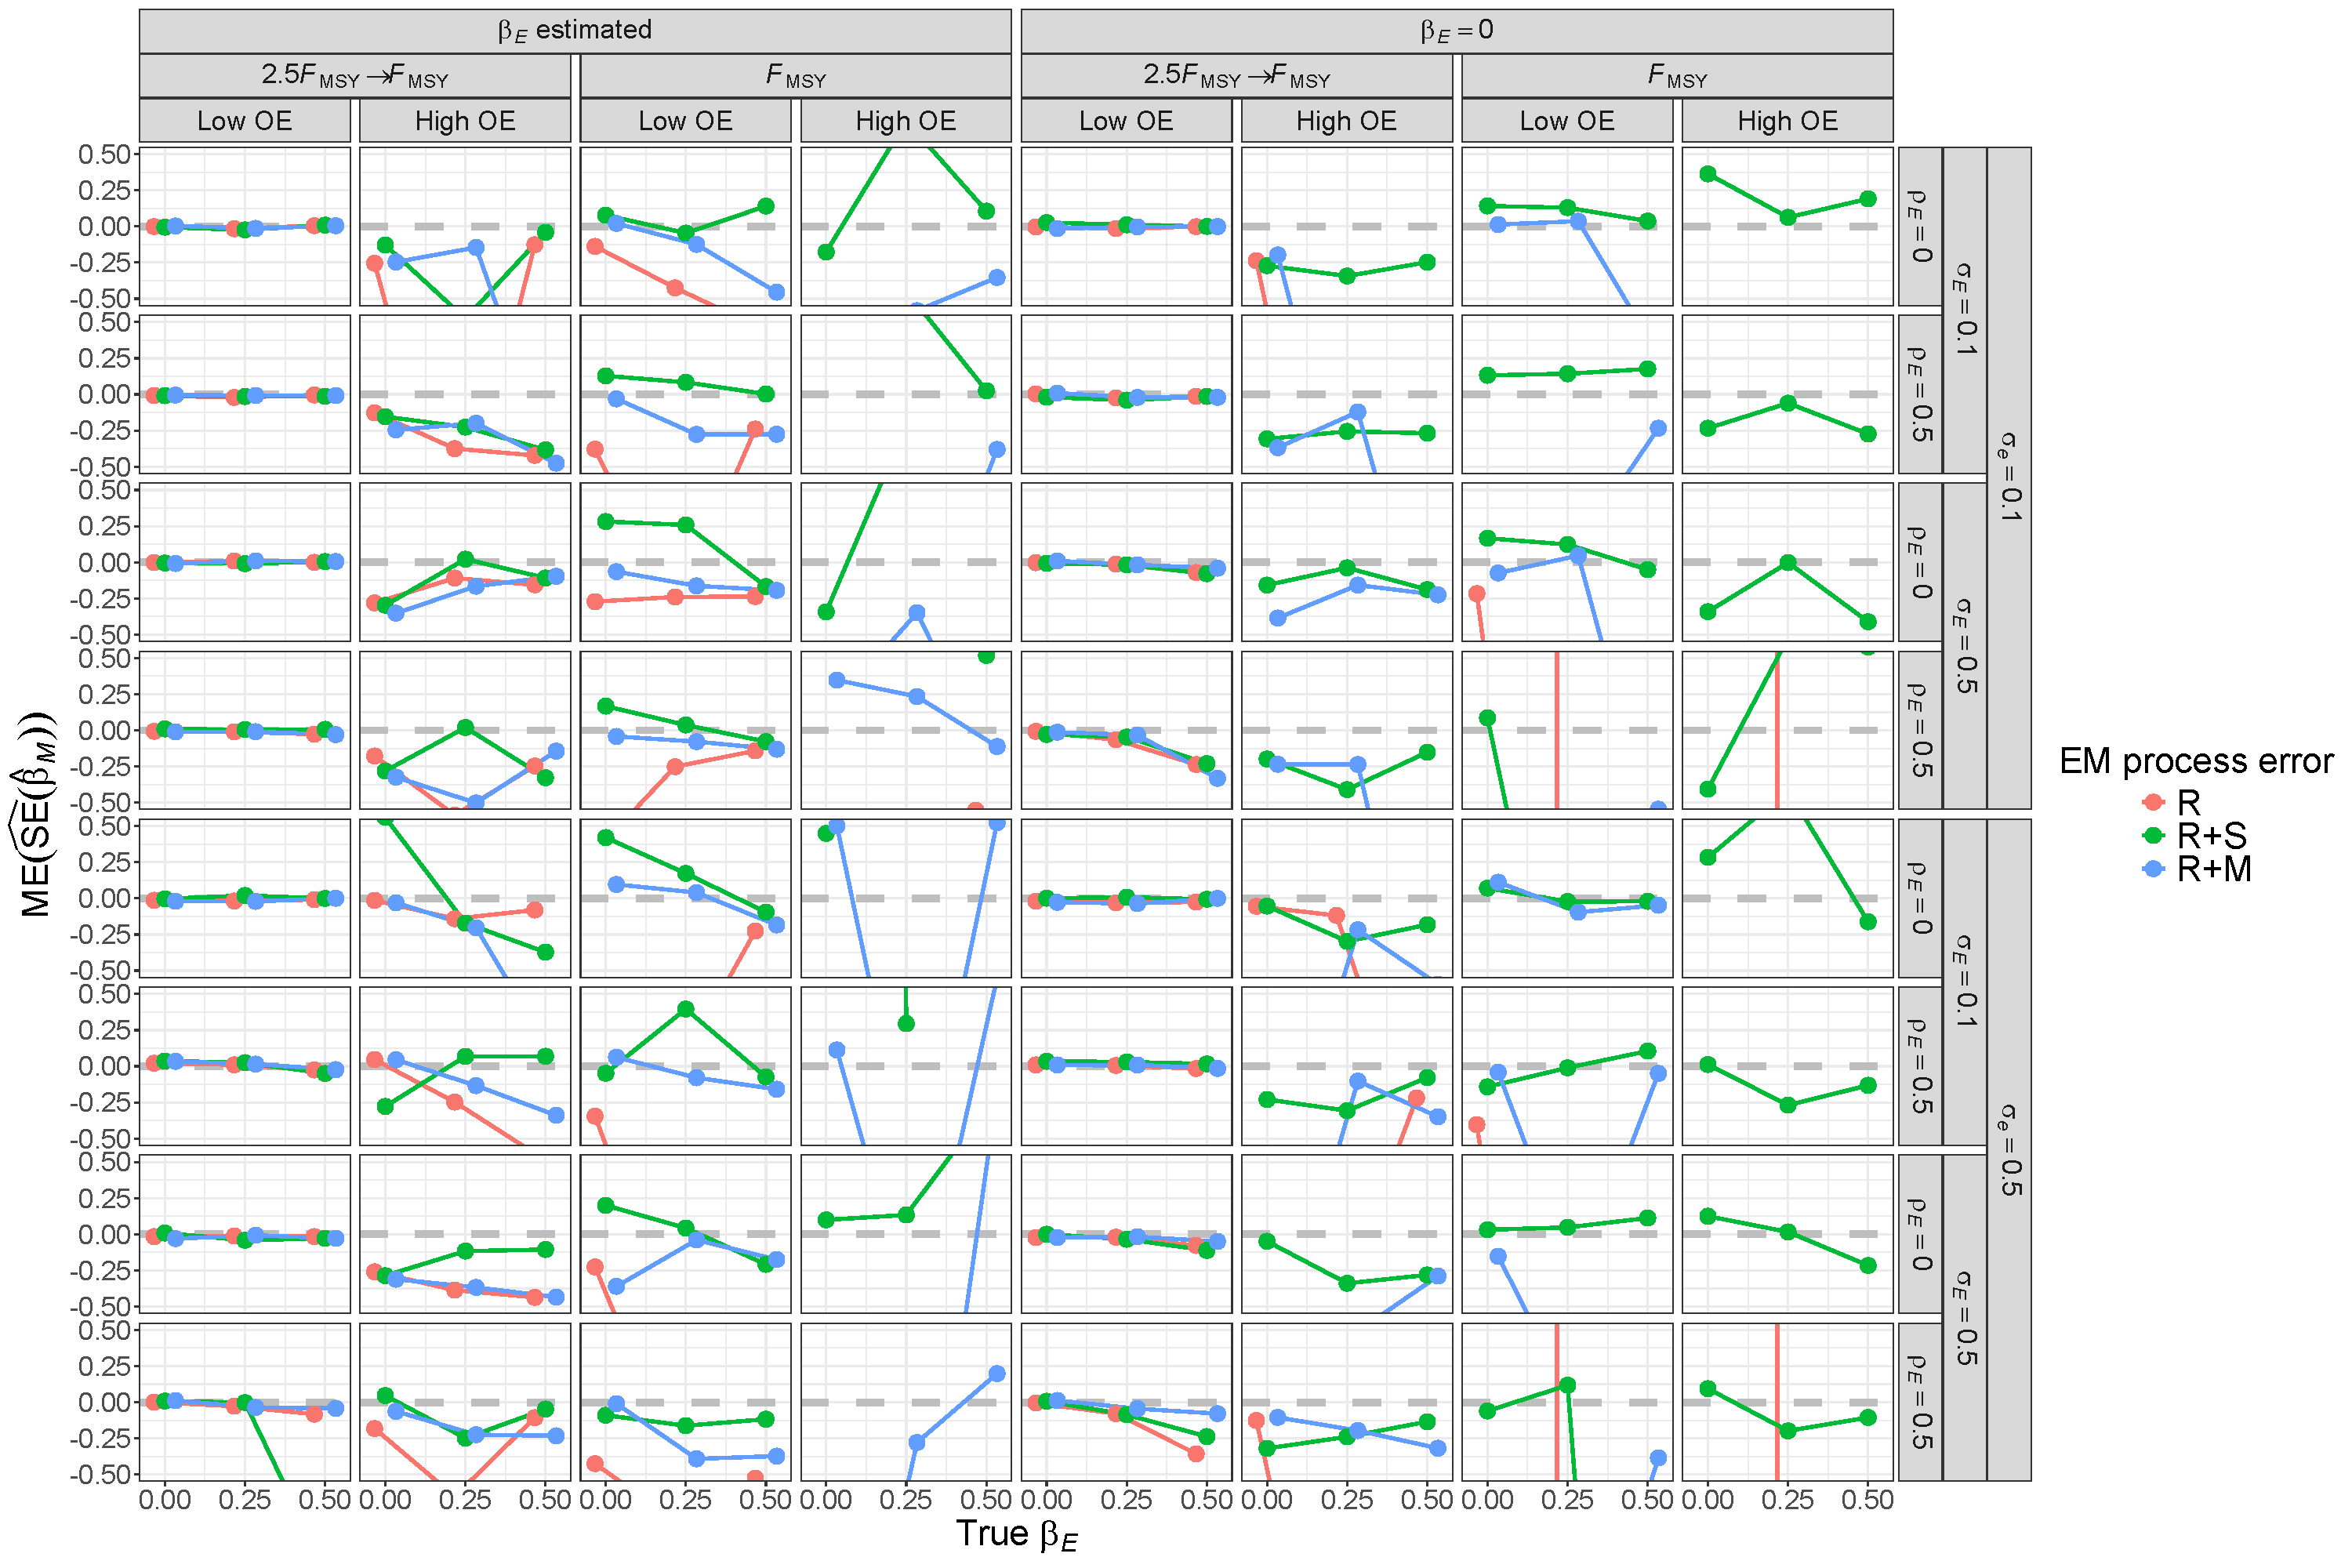
\includegraphics[height = \textheight]{se_beta_M_bias_Rom}
\end{center}
\caption{For R operating models, median error (ME) of Hessian-based estimates of standard error for median $M$ parameter ($\beta_M$) from fitting estimating models with alternative process error assumptions and treatment of the covariate effect ($\beta_ E= 0$ or estimated). True standard error is defined as the mean of the standard error estimates accross converged fits to simulated data sets for a given operating model scenario.}\label{se_beta_M_bias_Rom}
\end{figure}
\end{landscape}

\begin{landscape}
\begin{figure}
\begin{center}
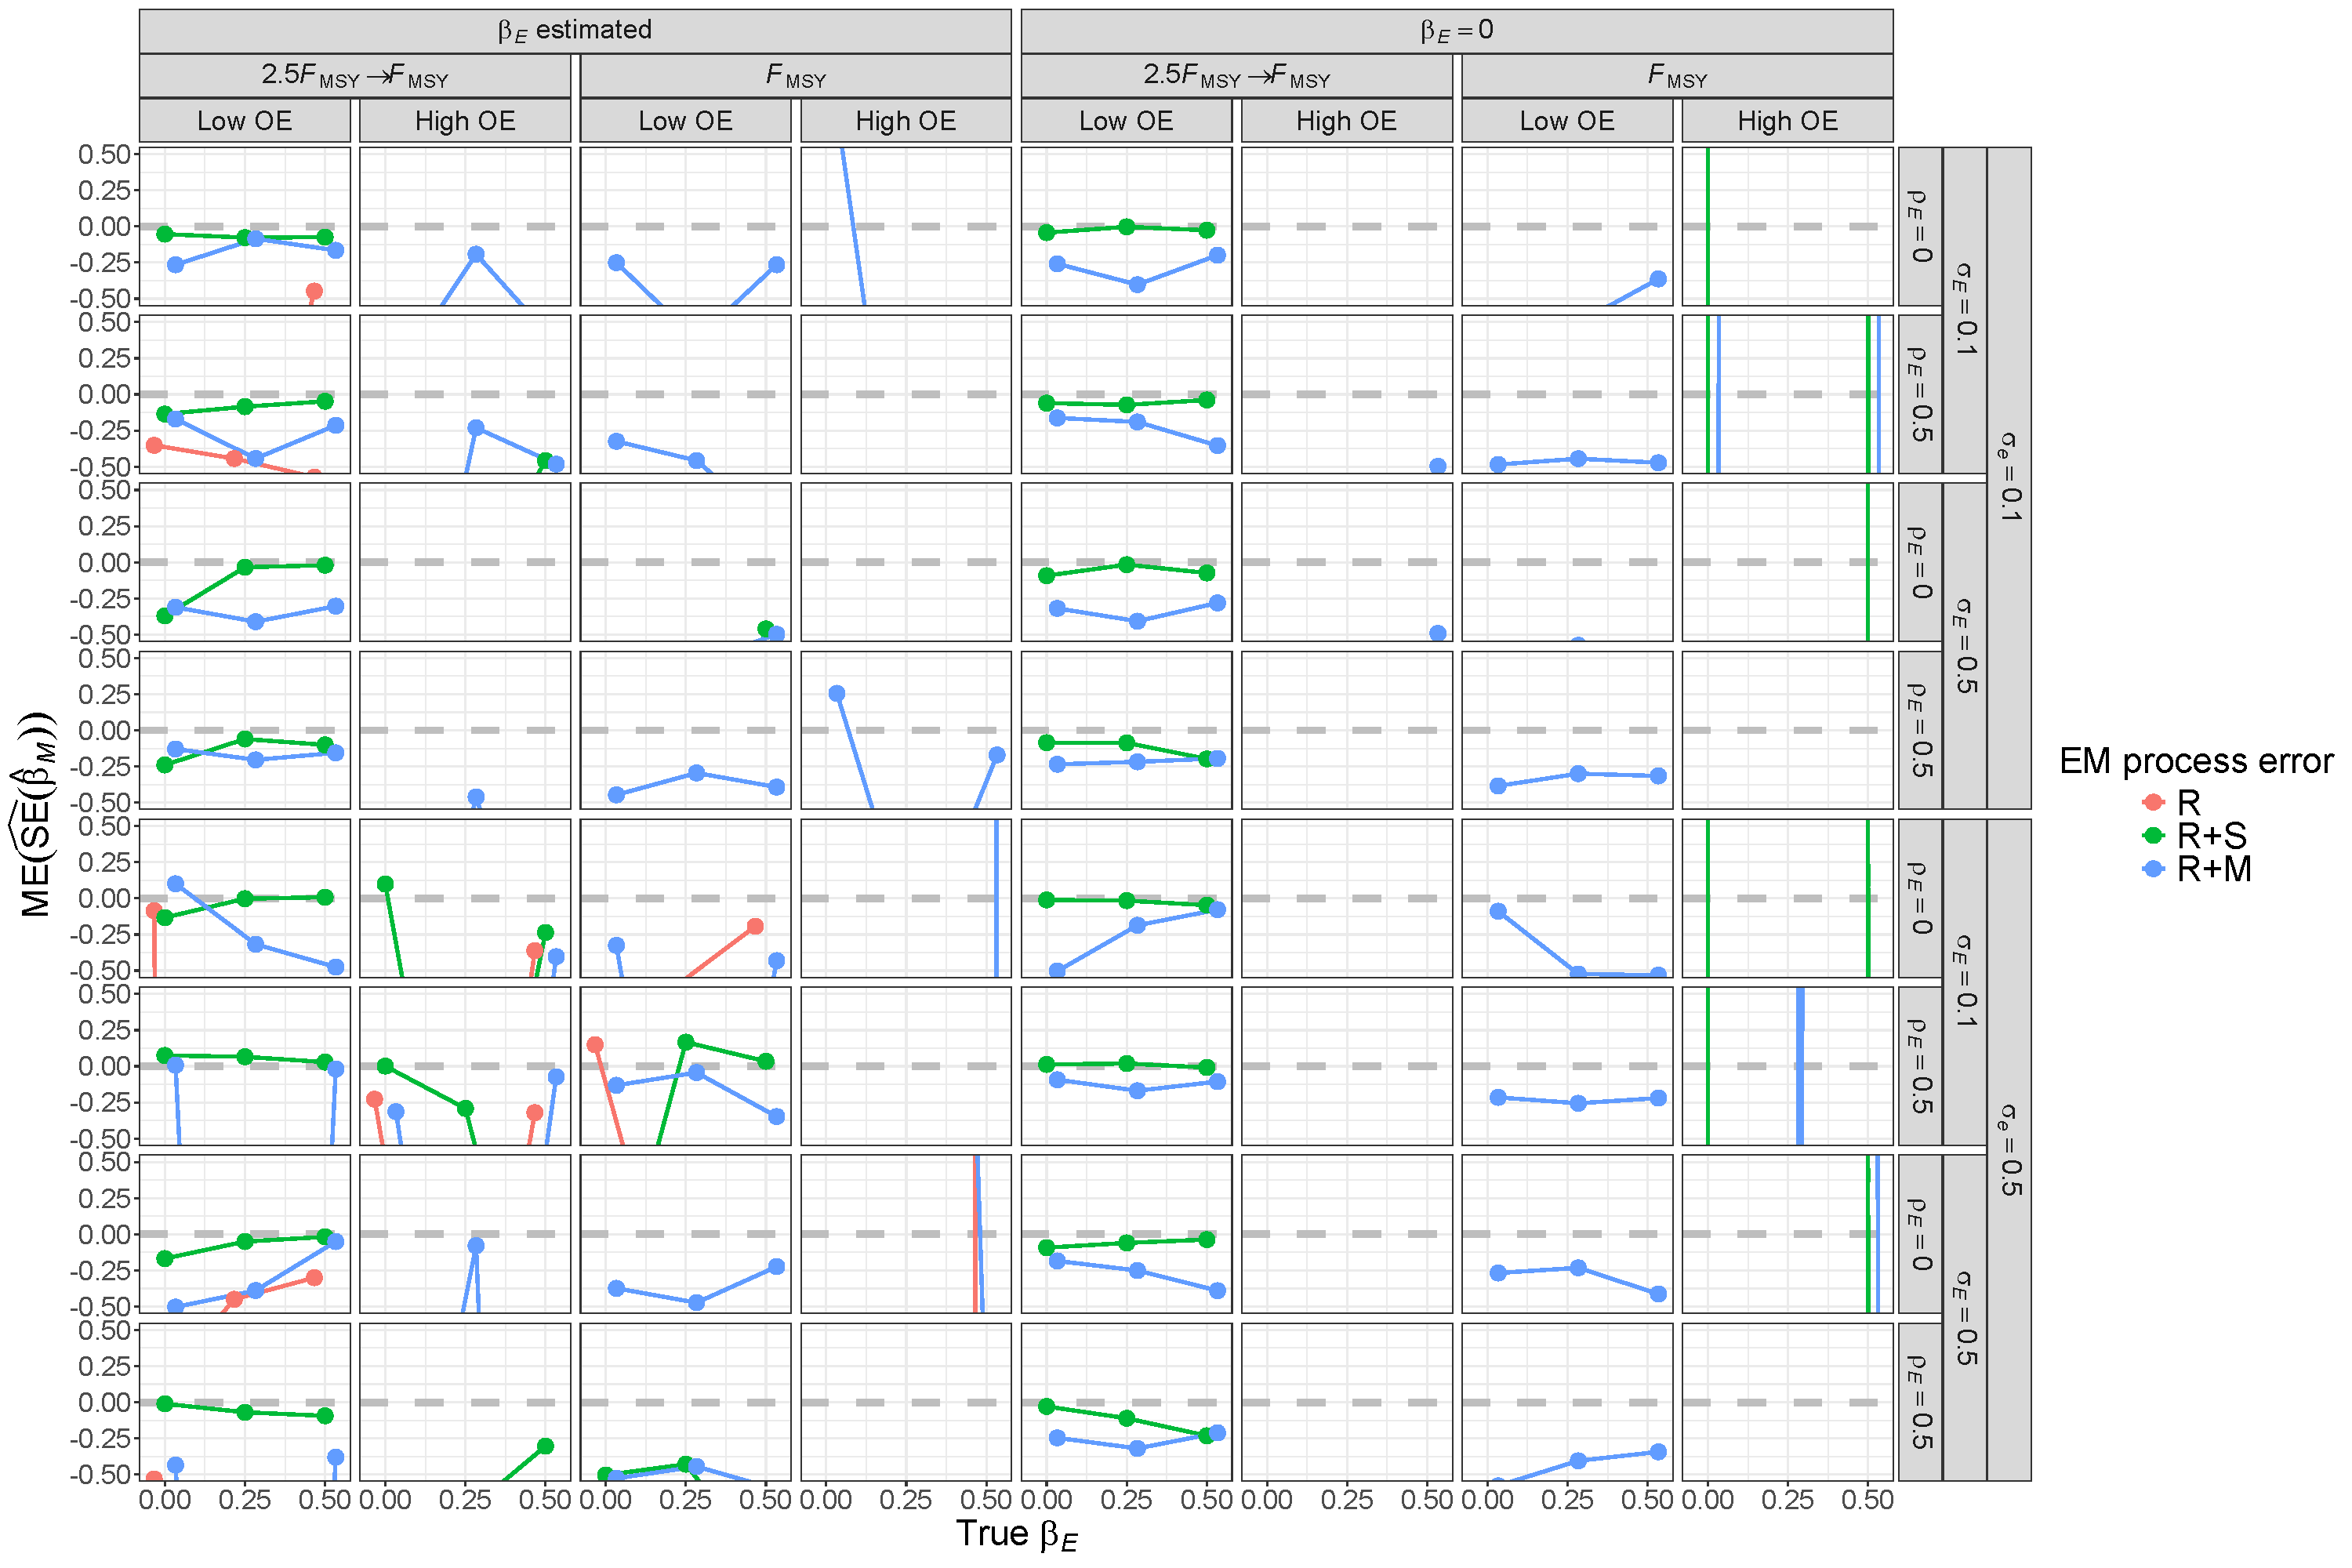
\includegraphics[height = \textheight]{se_beta_M_bias_RSom}
\end{center}
\caption{For R+S operating models, median error (ME) of Hessian-based estimates of standard error for median $M$ parameter ($\beta_M$) from fitting estimating models with alternative process error assumptions and treatment of the covariate effect ($\beta_ E= 0$ or estimated). True standard error is defined as the mean of the standard error estimates accross converged fits to simulated data sets for a given operating model scenario.}\label{se_beta_M_bias_RSom}
\end{figure}
\end{landscape}

\begin{landscape}
\begin{figure}
\begin{center}
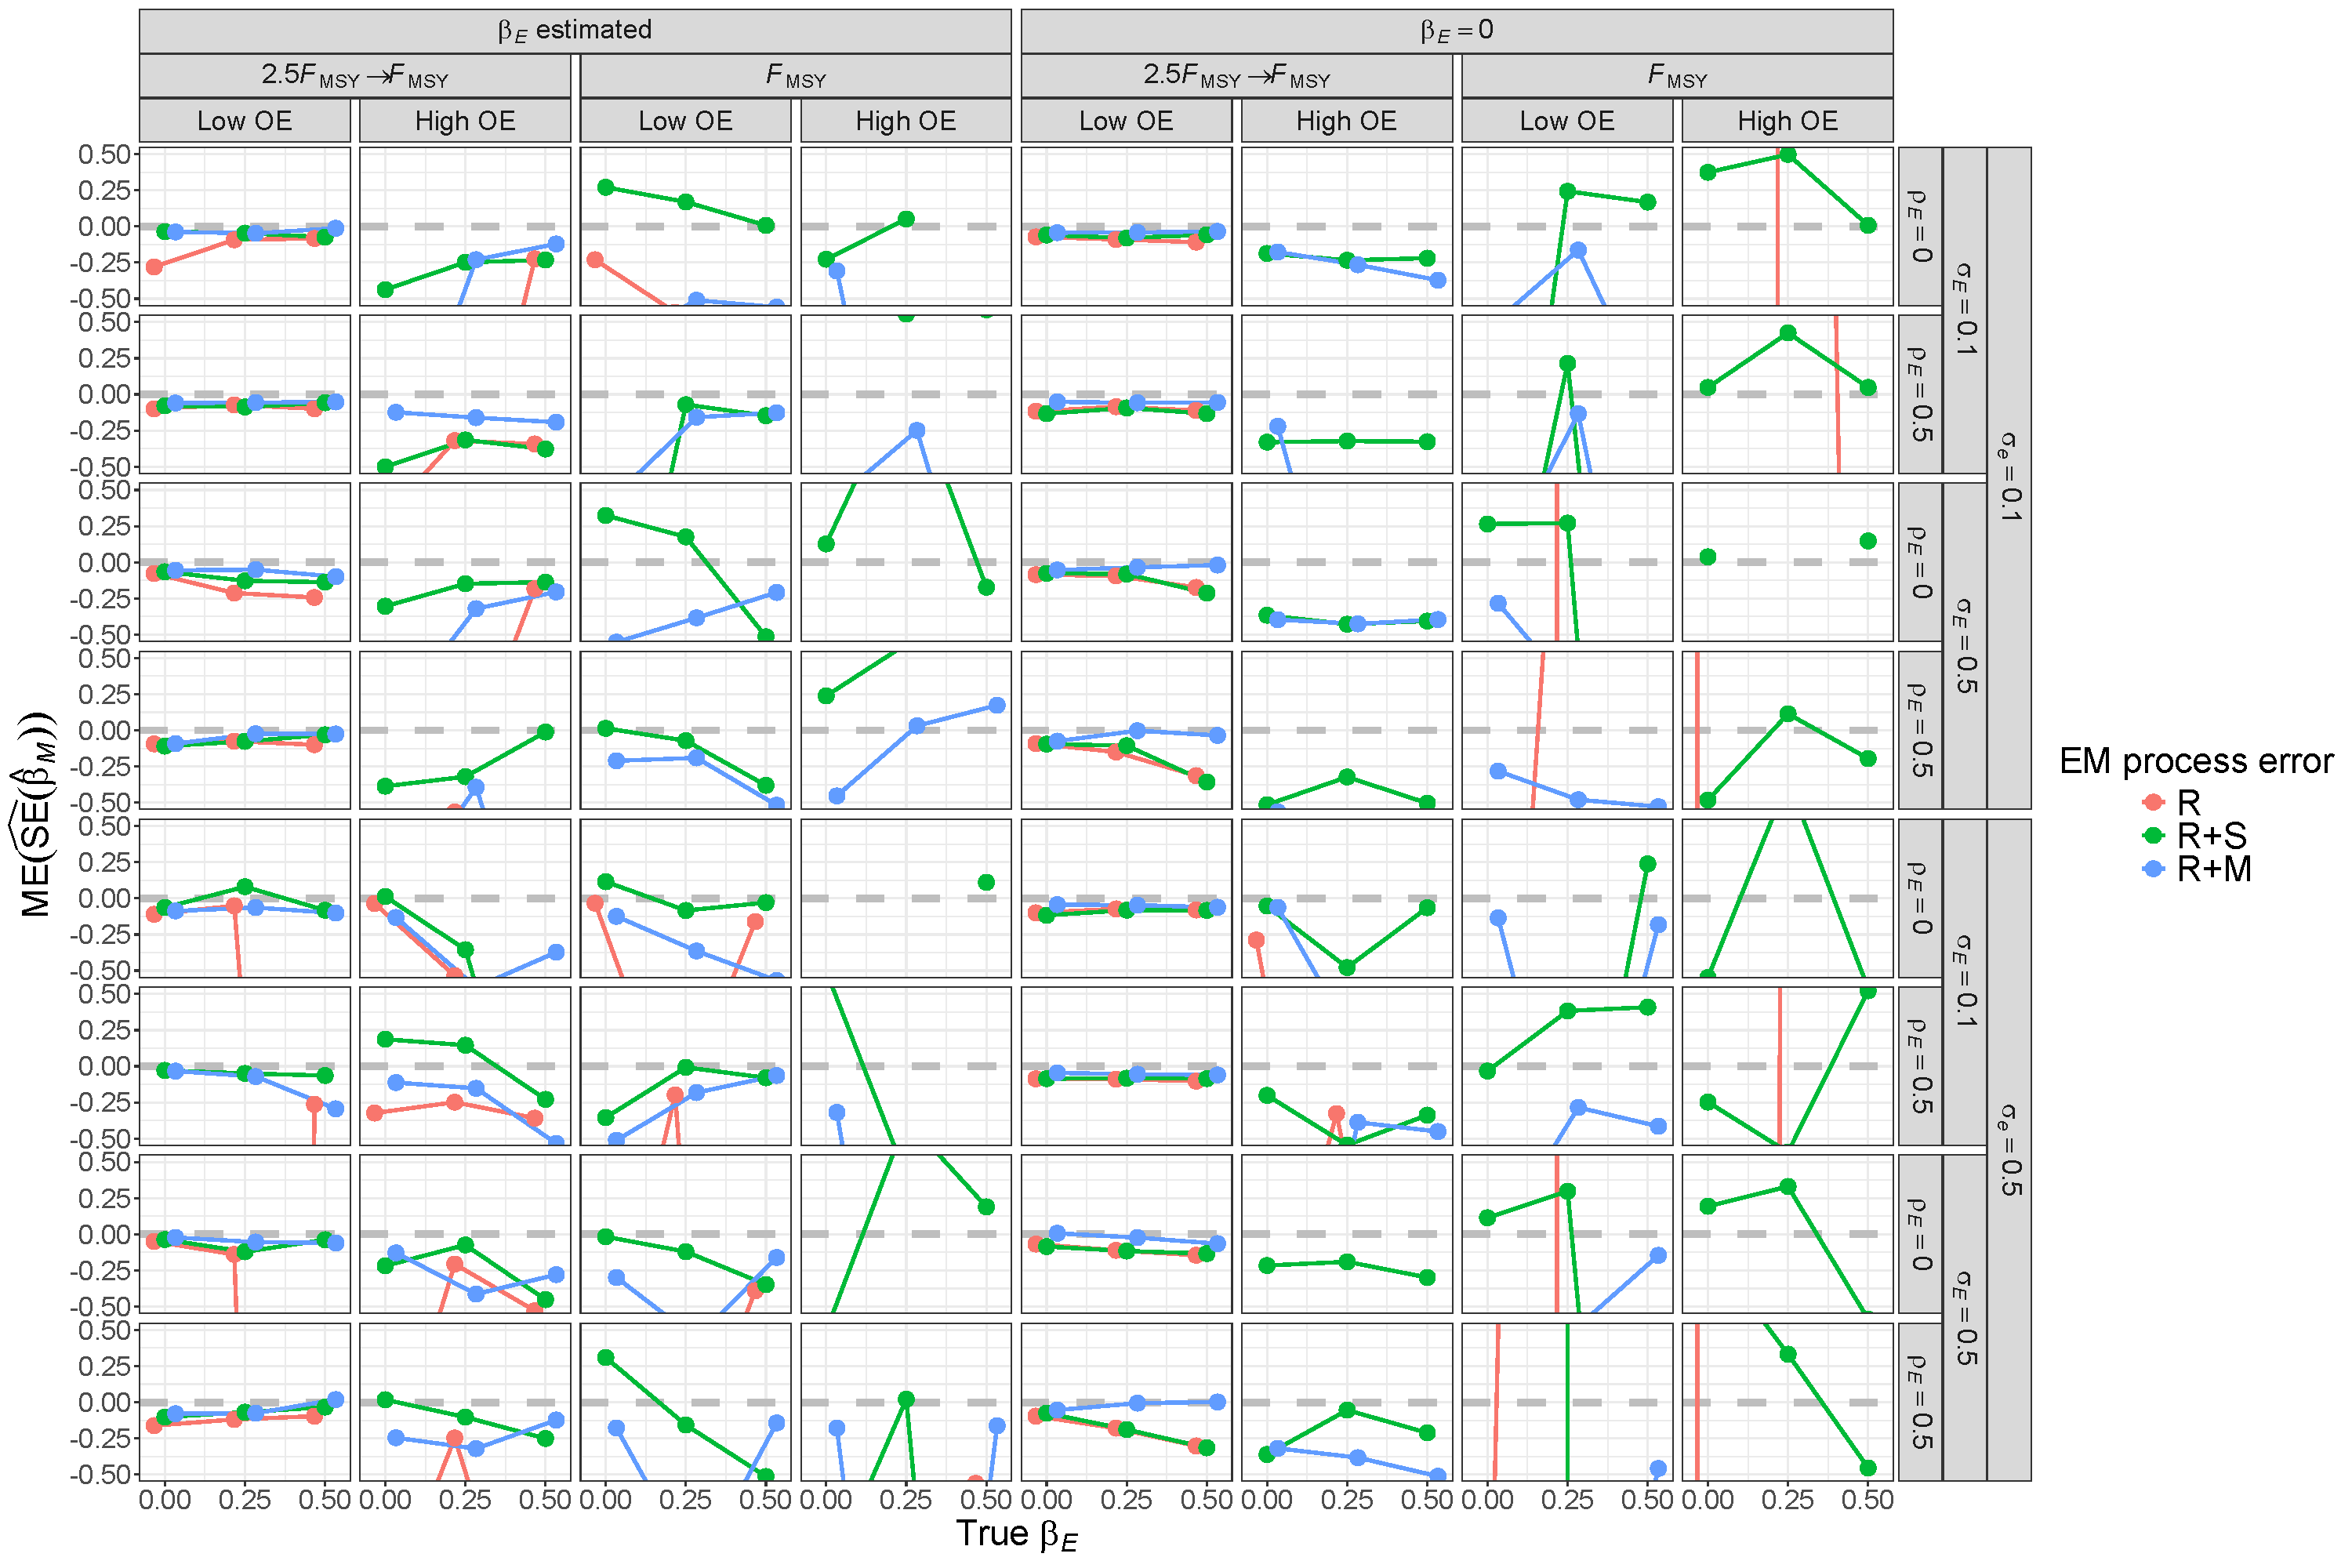
\includegraphics[height = \textheight]{se_beta_M_bias_RMom}
\end{center}
\caption{For R+M operating models, median error (ME) of Hessian-based estimates of standard error for median $M$ parameter ($\beta_M$) from fitting estimating models with alternative process error assumptions and treatment of the covariate effect ($\beta_ E= 0$ or estimated). True standard error is defined as the mean of the standard error estimates accross converged fits to simulated data sets for a given operating model scenario.}\label{se_beta_M_bias_RMom}
\end{figure}
\end{landscape}

\begin{landscape}
\begin{figure}
\begin{center}
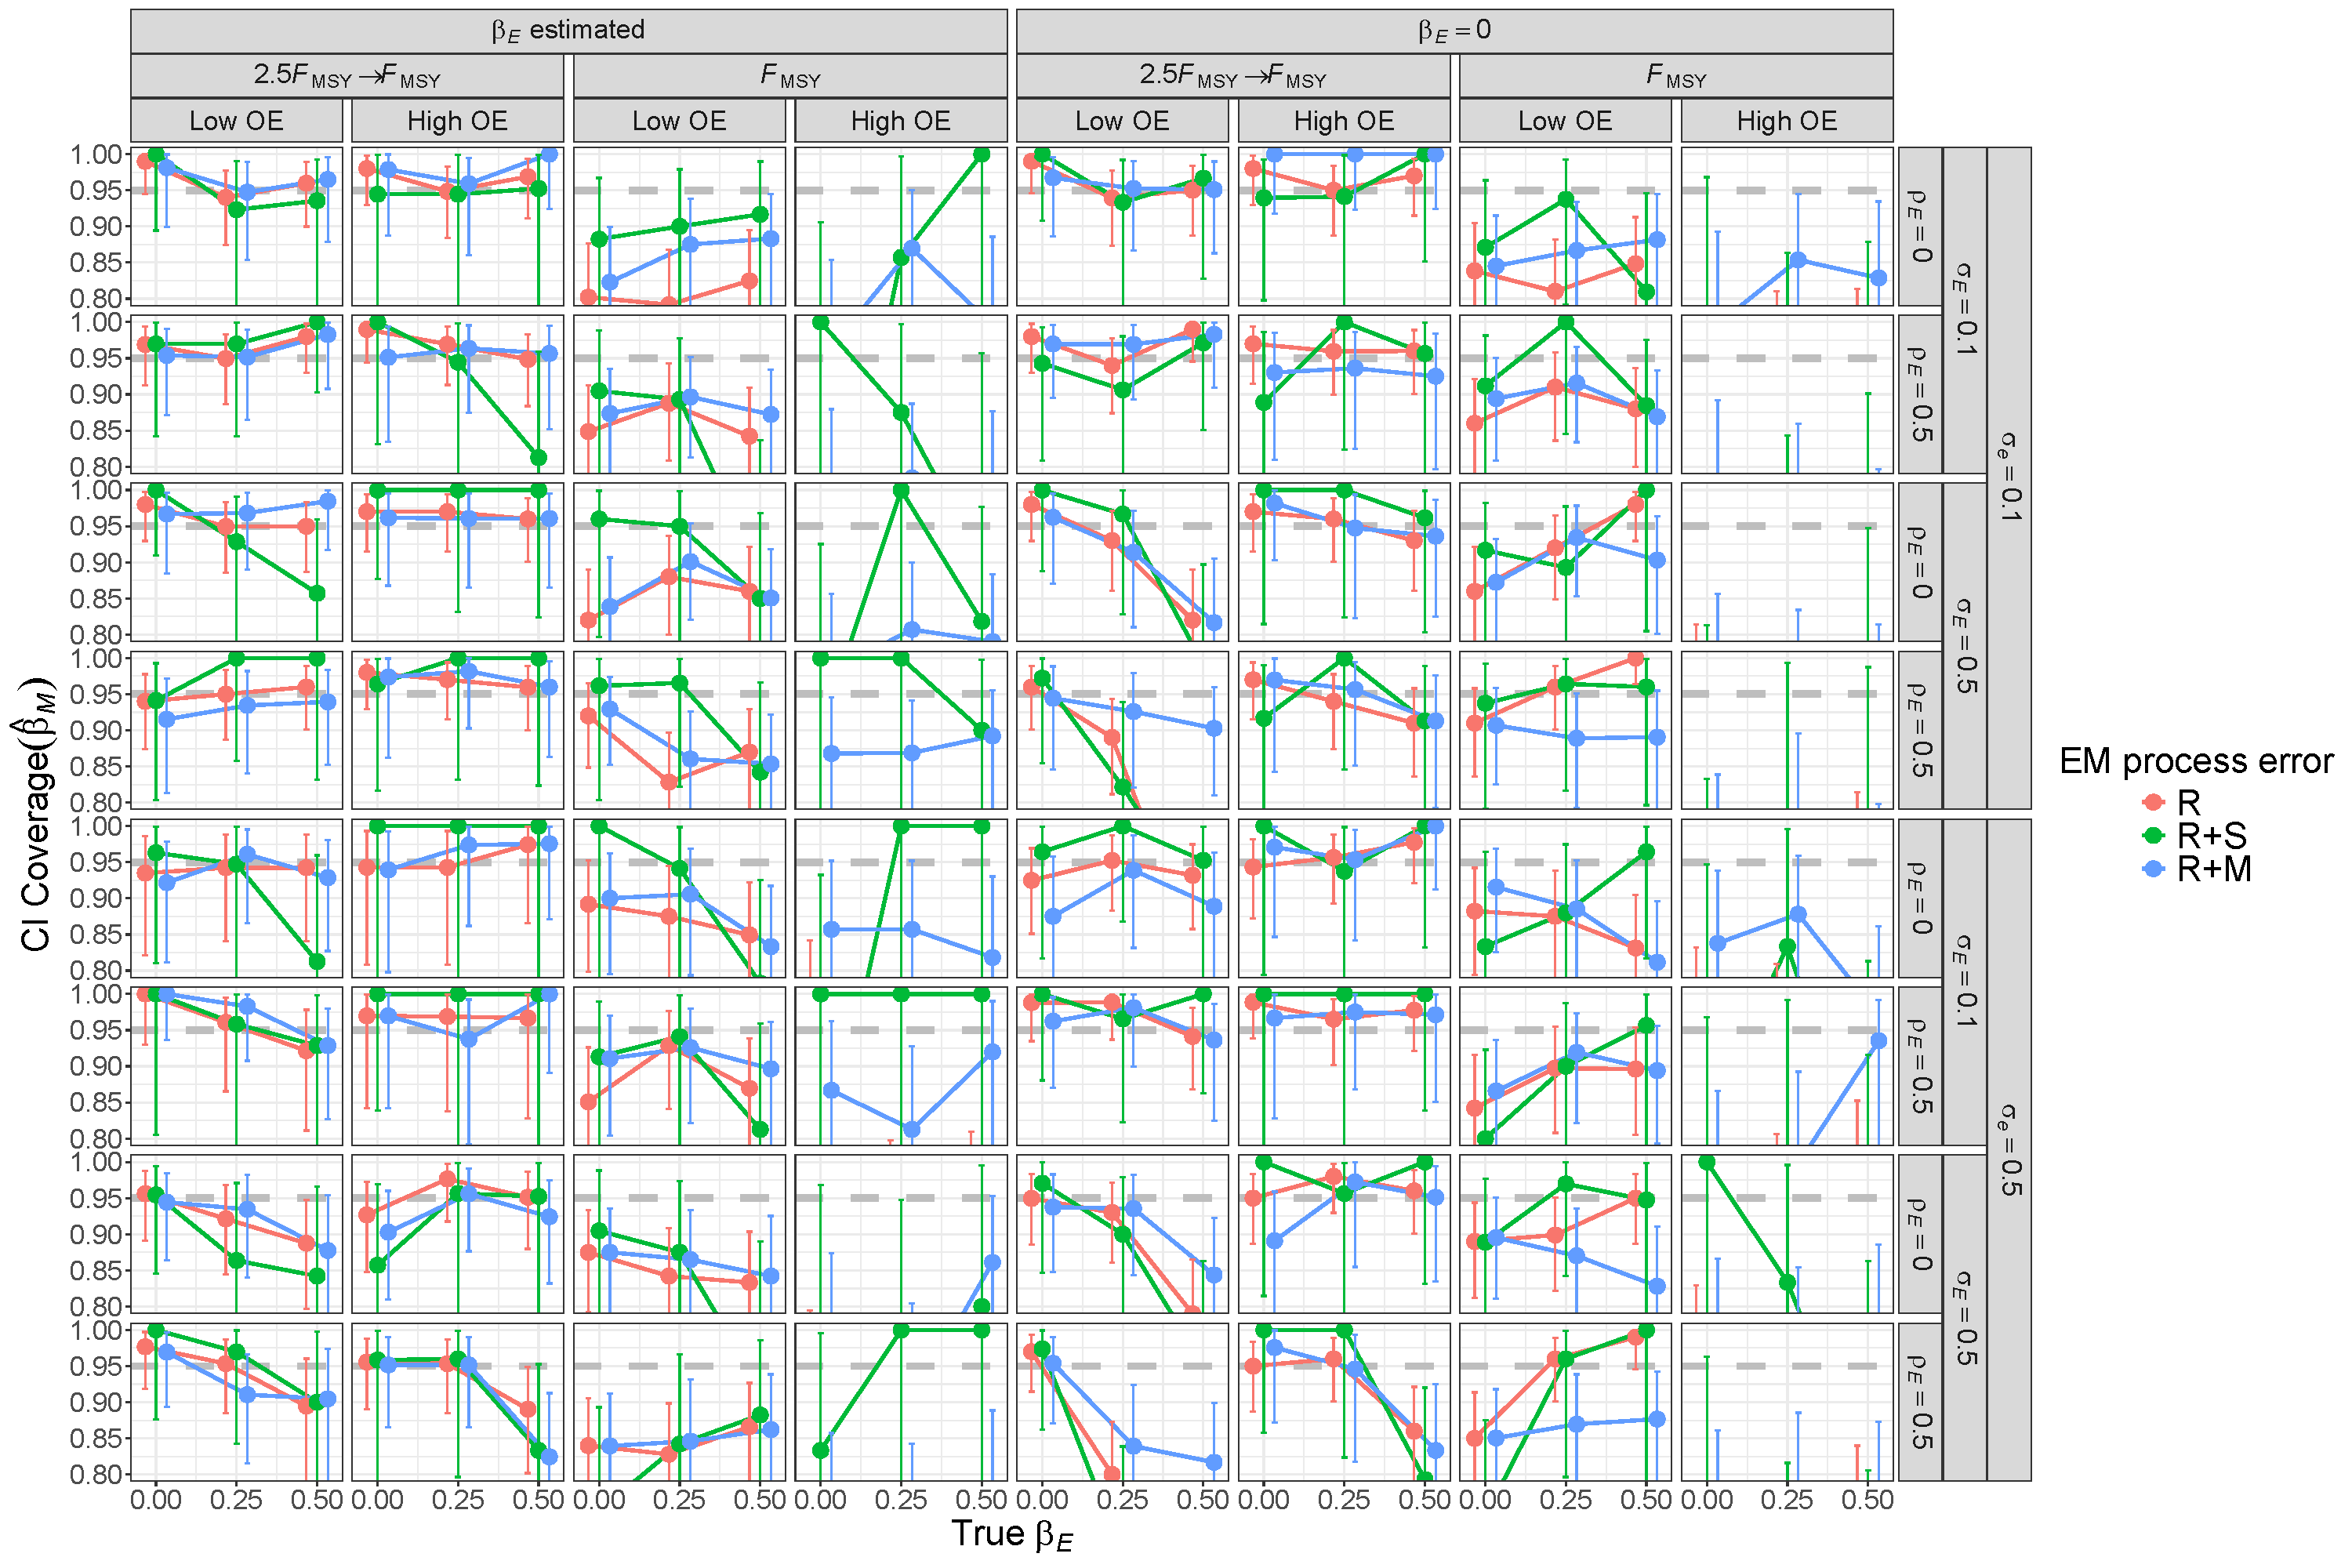
\includegraphics[height = \textheight]{beta_M_CI_coverage_Rom}
\end{center}
\caption{For R operating models, probability of 95\% confidence interval for $\beta_M$ containing the true value for estimating models with alternative process error assumptions and treatment of covariate effect ($\beta_E = 0$ or estimated). Vertical lines represent 95\% confidence intervals.}\label{beta_M_CI_coverage_Rom}
\end{figure}
\end{landscape}

\begin{landscape}
\begin{figure}
\begin{center}
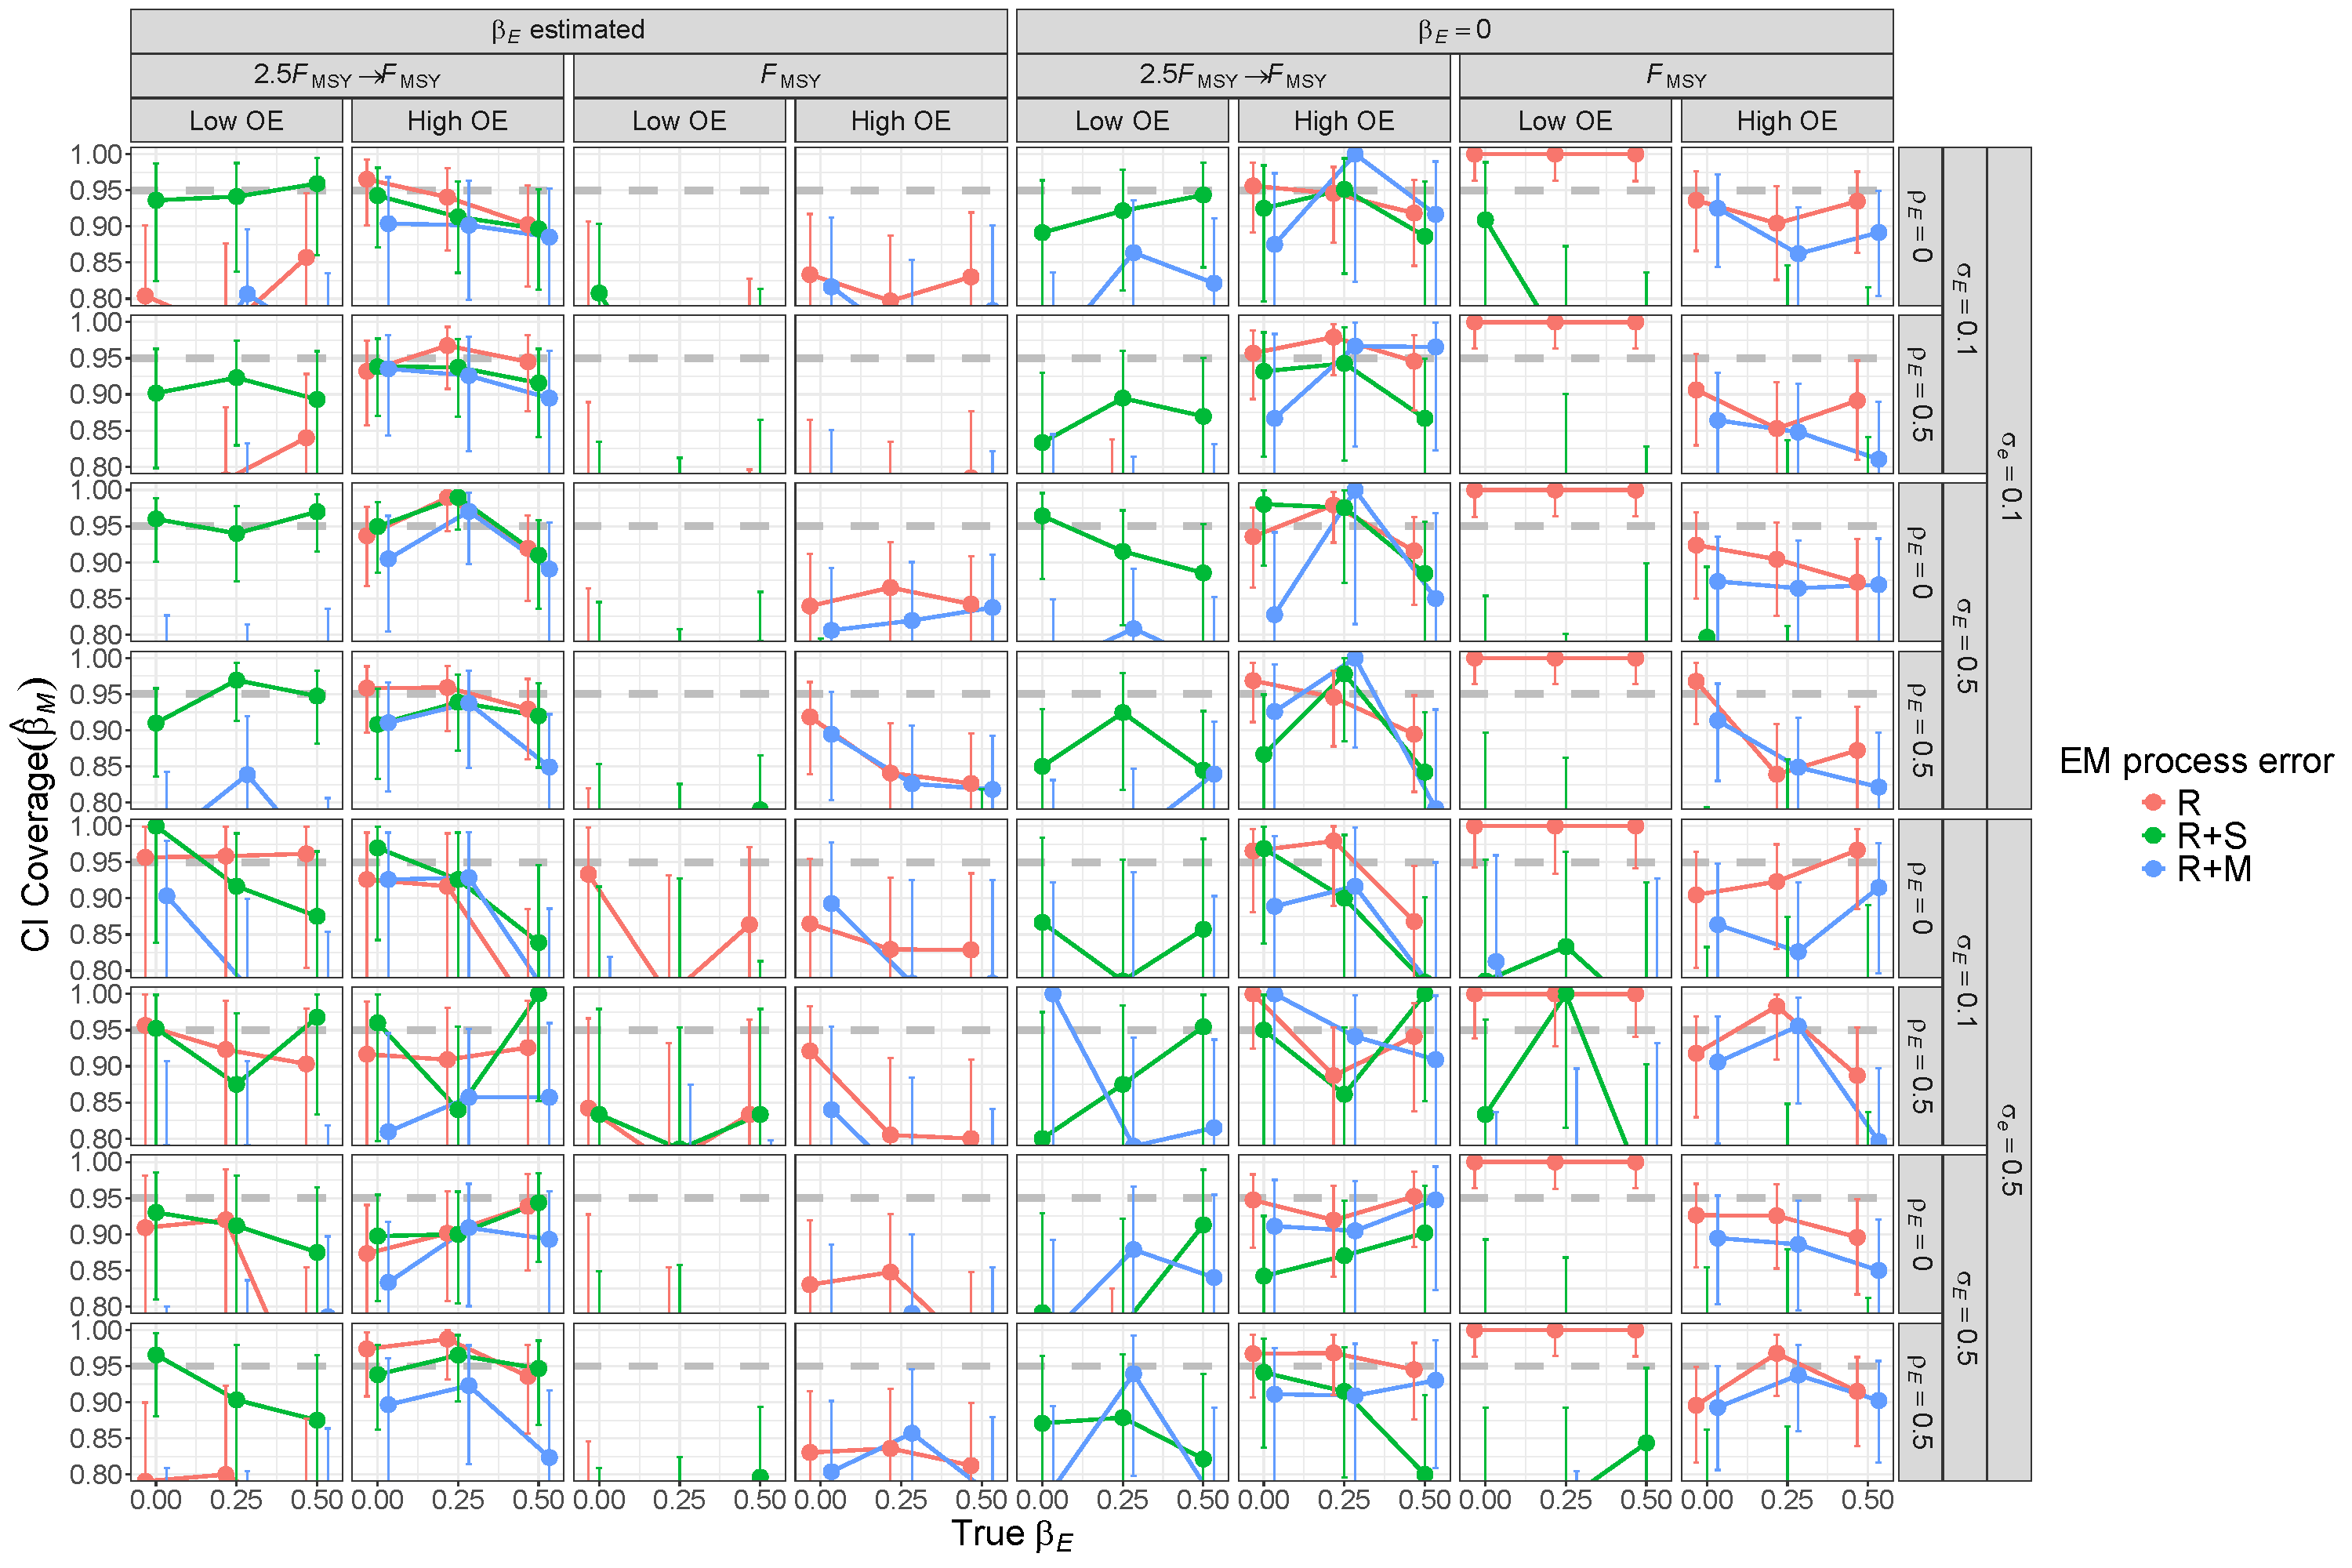
\includegraphics[height = \textheight]{beta_M_CI_coverage_RSom}
\end{center}
\caption{For R+S operating models, probability of 95\% confidence interval for $\beta_M$ containing the true value for estimating models with alternative process error assumptions and treatment of covariate effect ($\beta_E = 0$ or estimated). Vertical lines represent 95\% confidence intervals.}\label{beta_M_CI_coverage_RSom}
\end{figure}
\end{landscape}

\begin{landscape}
\begin{figure}
\begin{center}
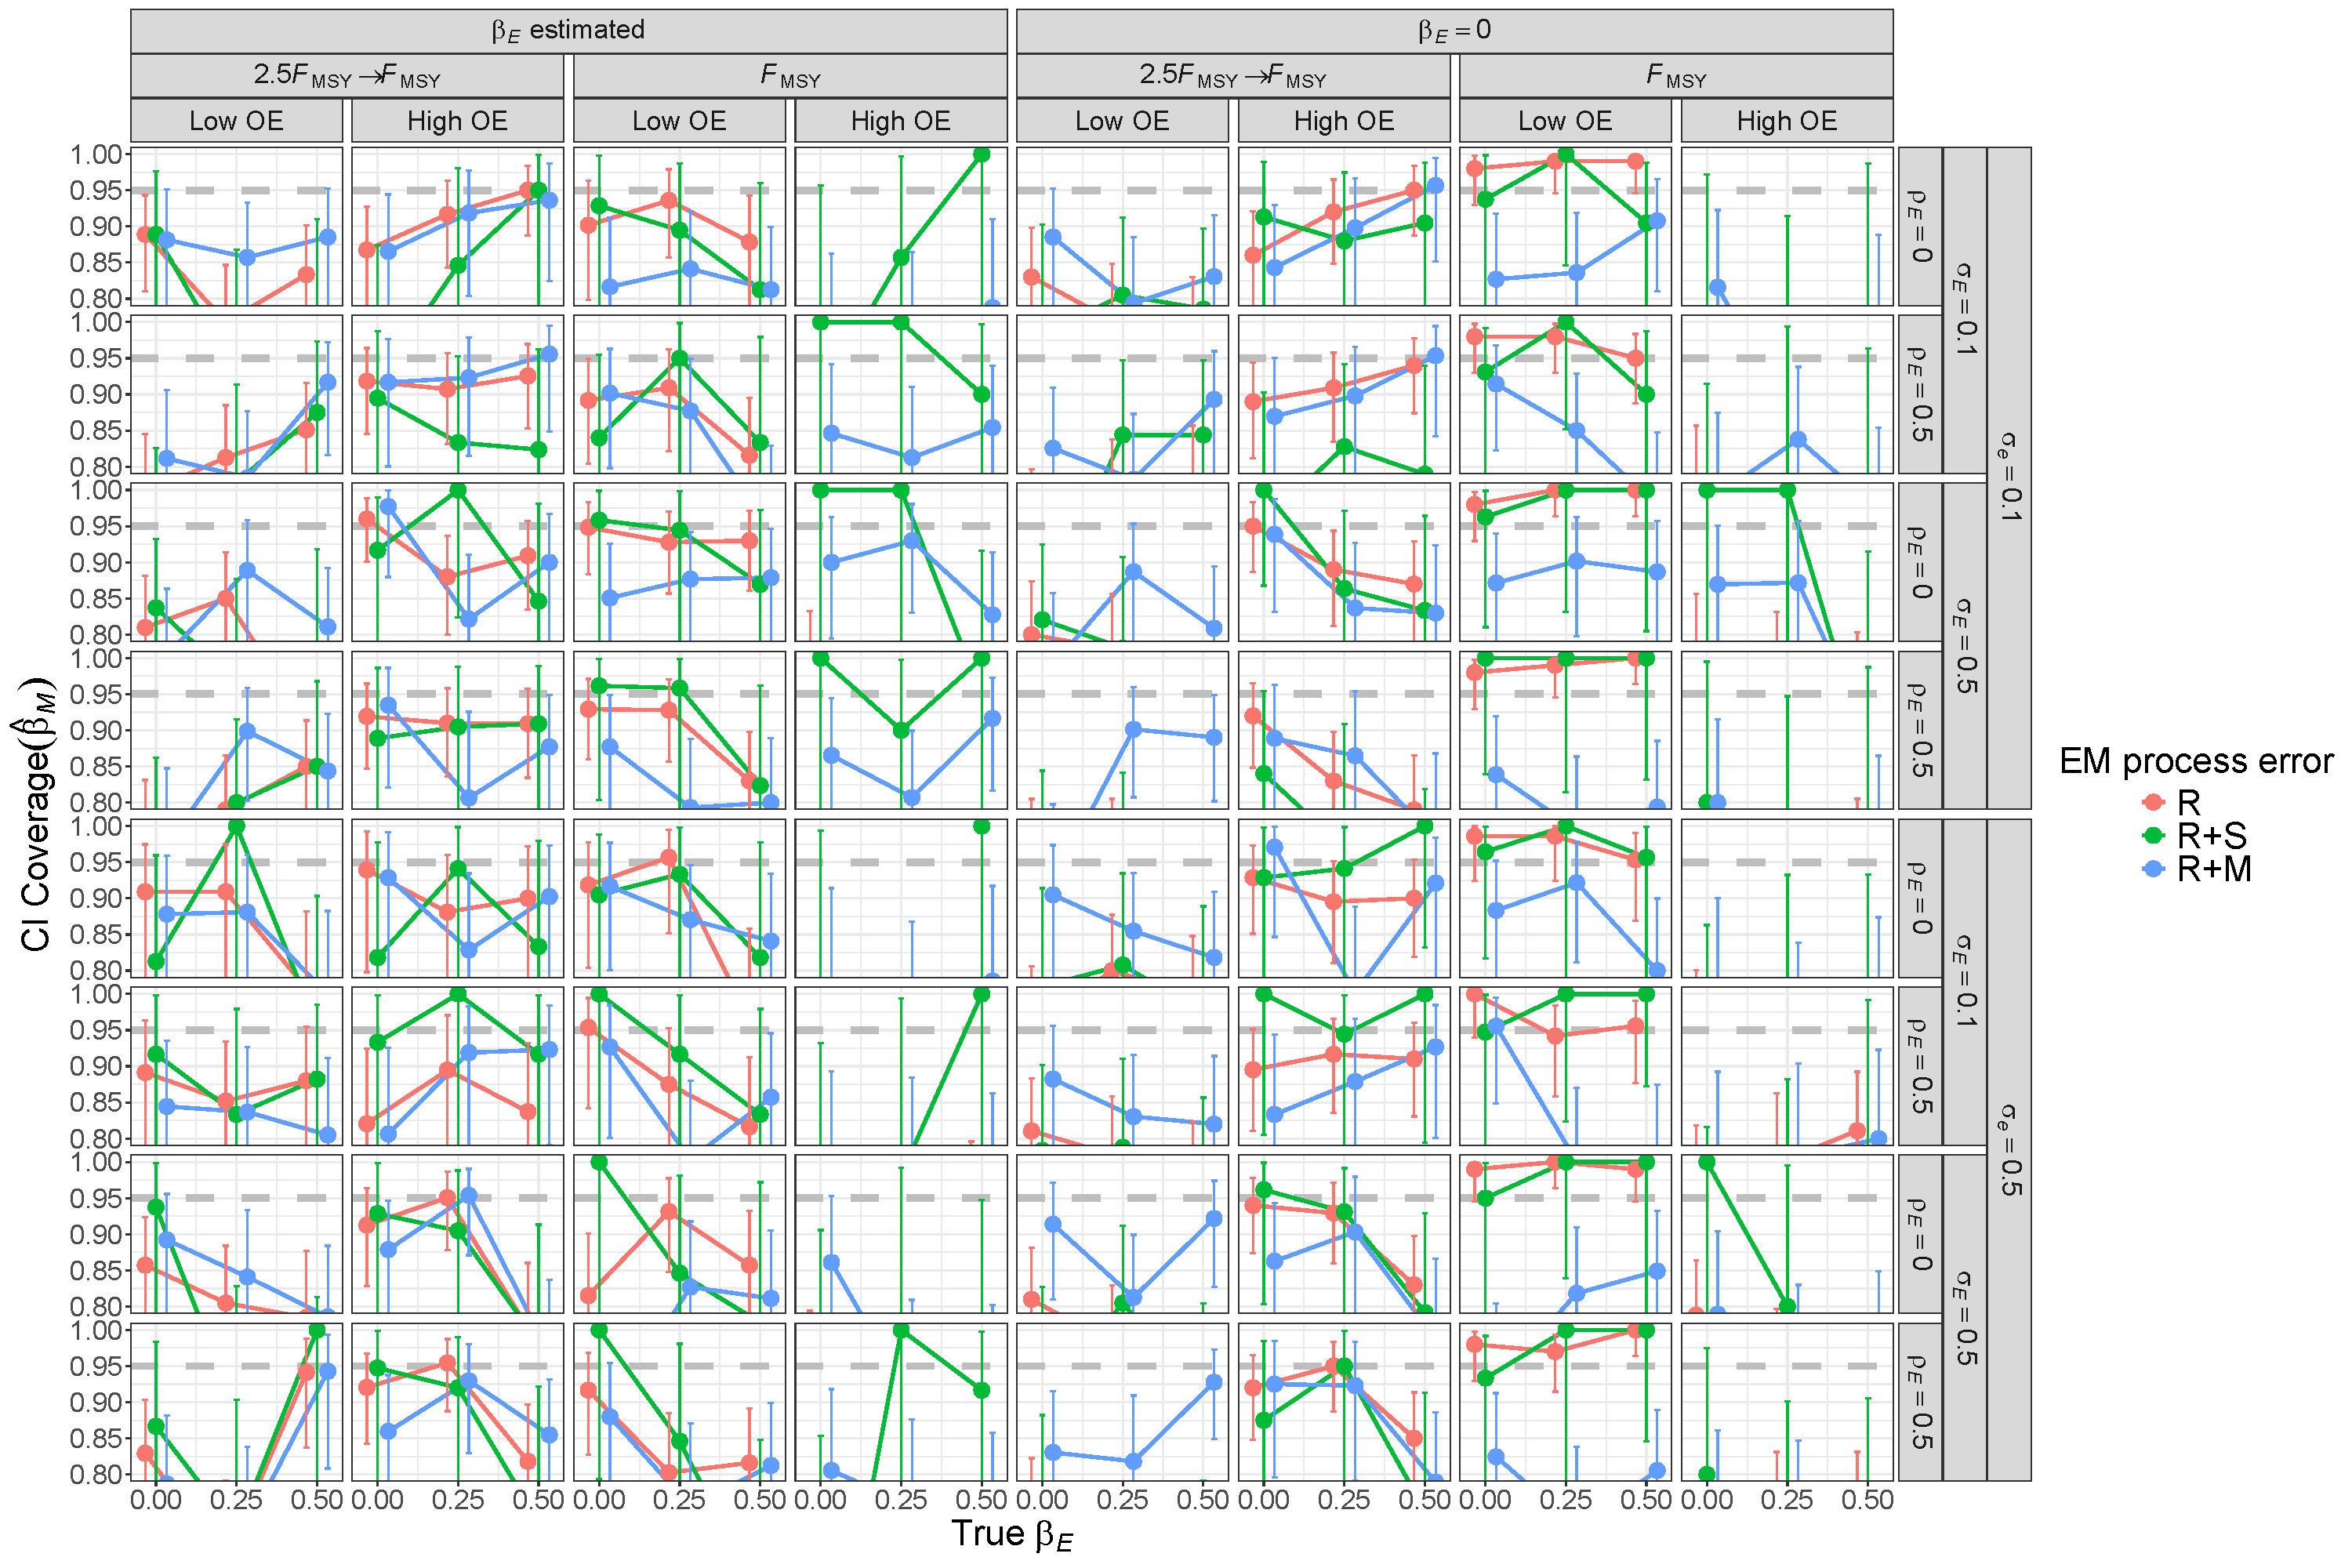
\includegraphics[height = \textheight]{beta_M_CI_coverage_RMom}
\end{center}
\caption{For R+M operating models, probability of 95\% confidence interval for $\beta_M$ containing the true value for estimating models with alternative process error assumptions and treatment of covariate effect ($\beta_E = 0$ or estimated). Vertical lines represent 95\% confidence intervals.}\label{beta_M_CI_coverage_RMom}
\end{figure}
\end{landscape}

\begin{landscape}
\begin{figure}
\begin{center}
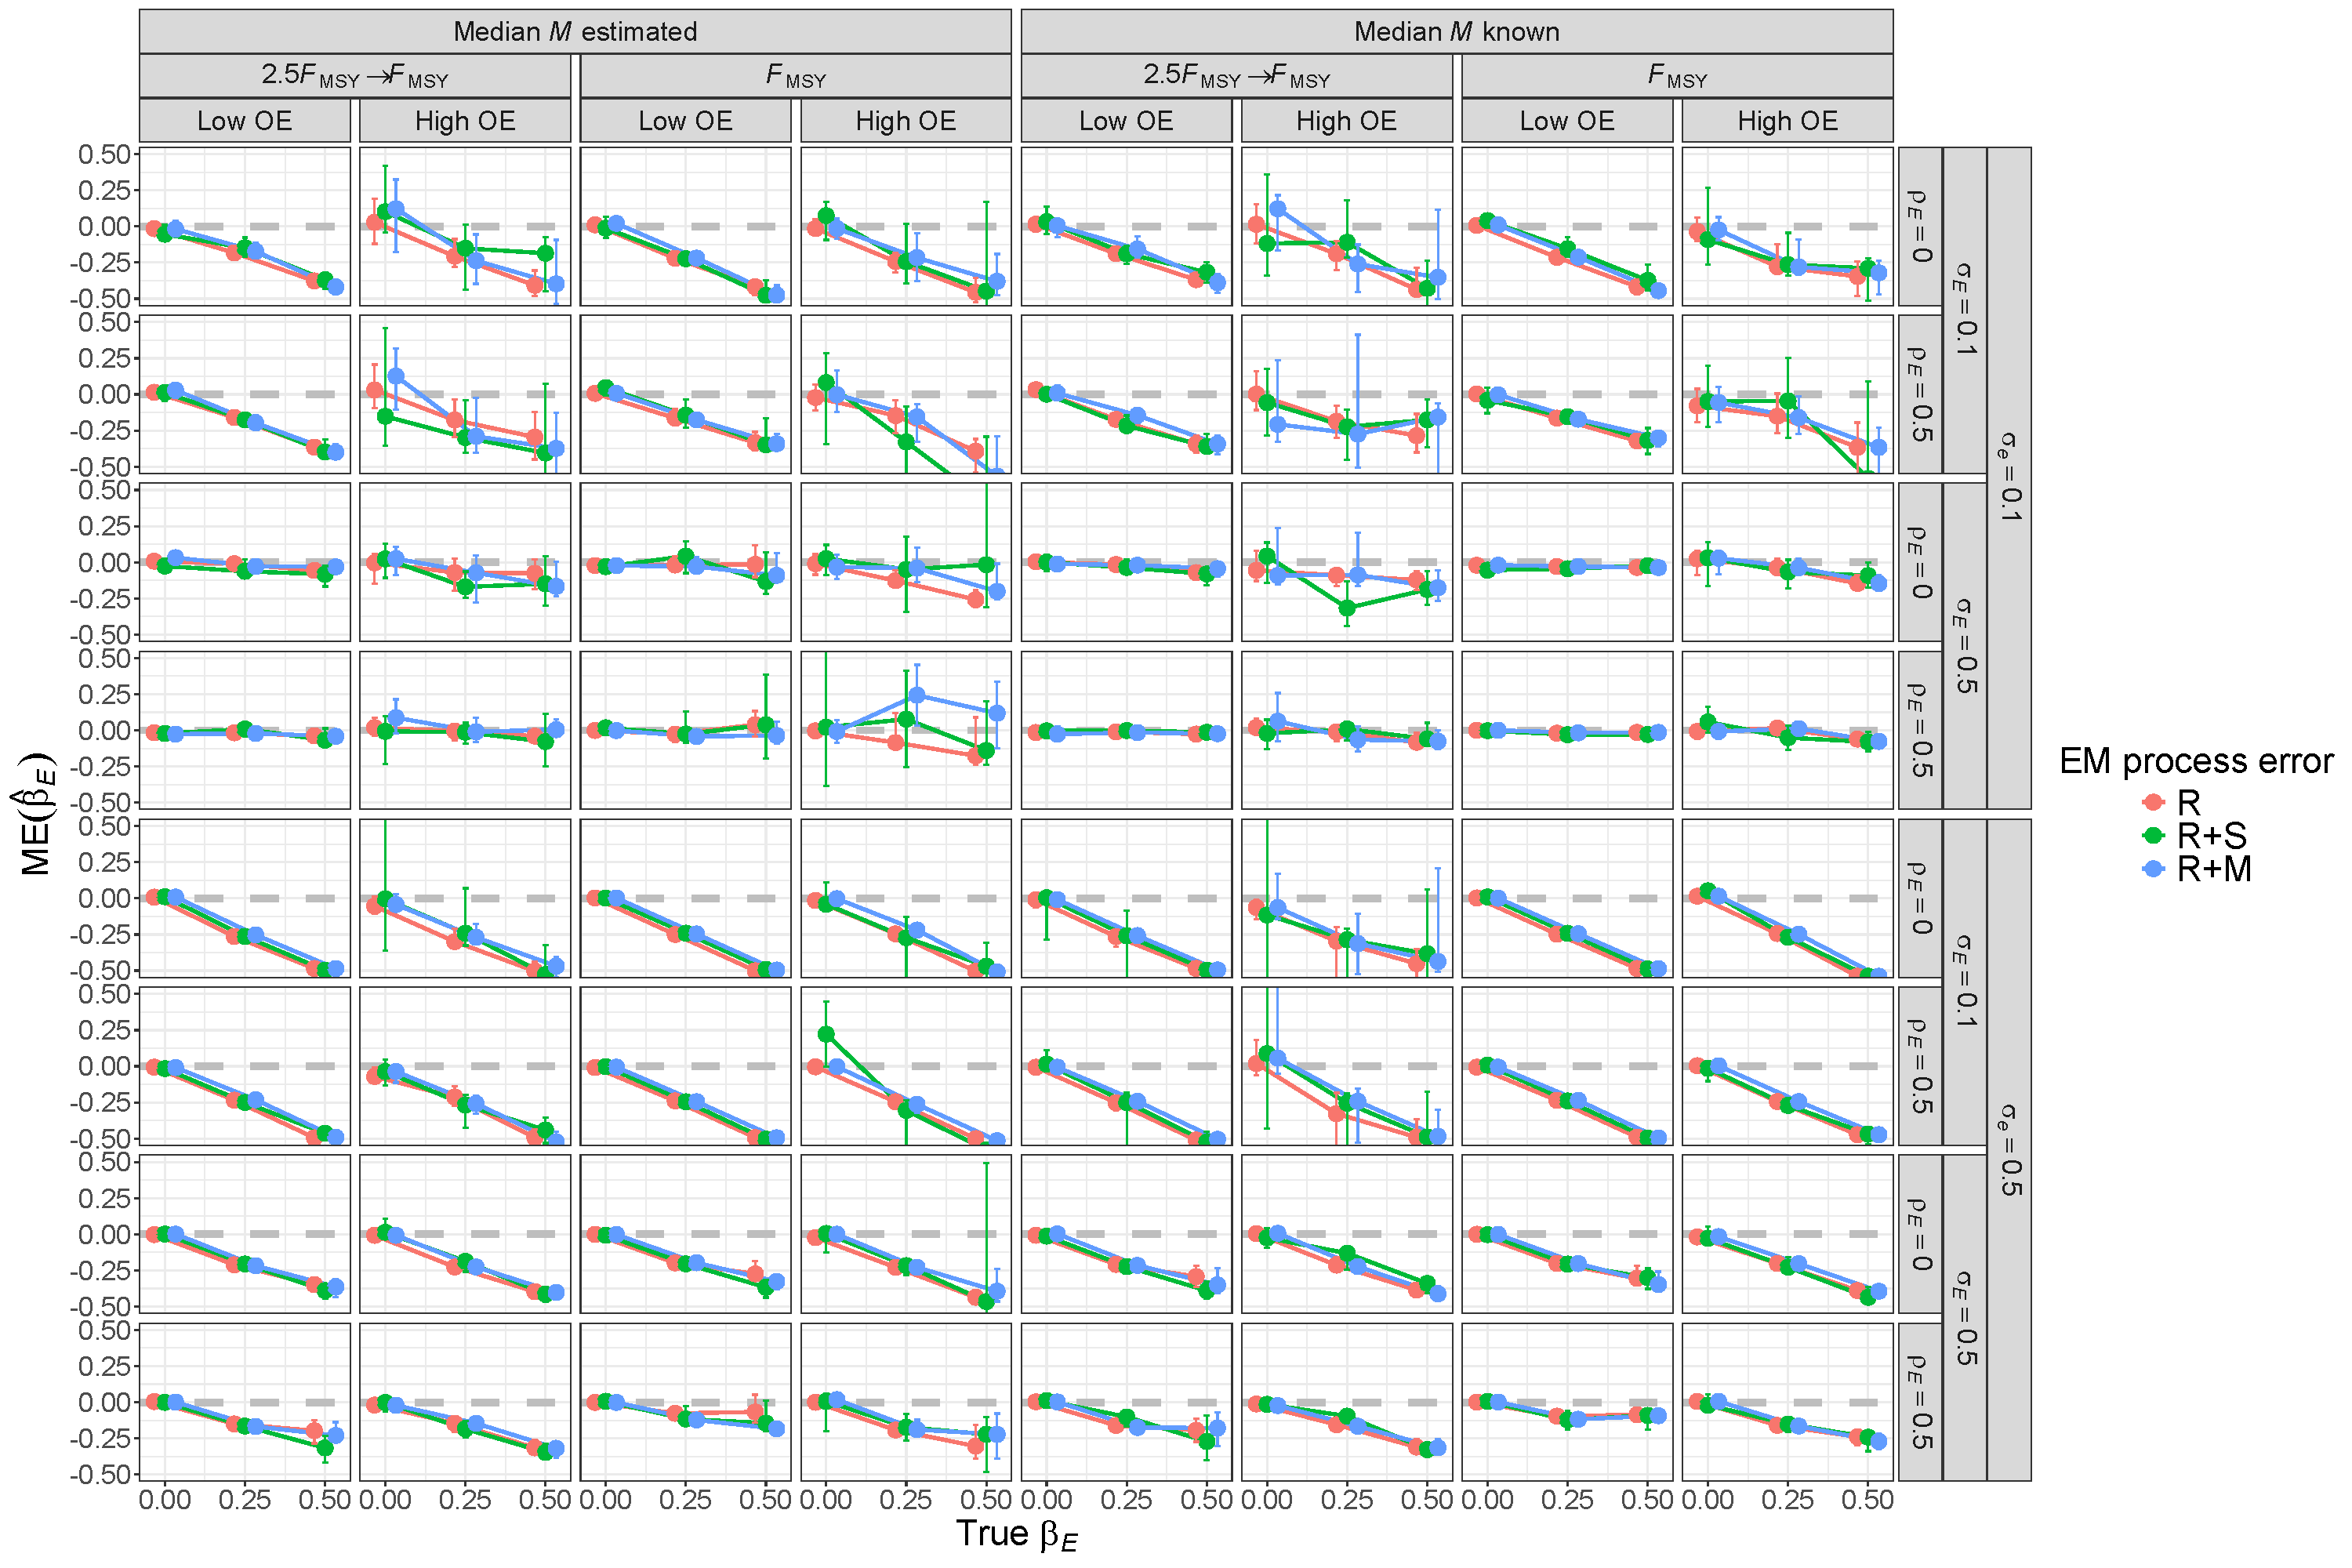
\includegraphics[height = \textheight]{beta_E_bias_Rom}
\end{center}
\caption{For R operating models, median error (ME) of estimates of environmental effect on $M$ ($\beta_E$) from fitting estimating models with alternative process error assumptions and treatment of median $M$ parameter ($\beta_M$). Vertical lines represent 95\% confidence intervals.}\label{beta_E_bias_Rom}
\end{figure}
\end{landscape}

\begin{landscape}
\begin{figure}
\begin{center}
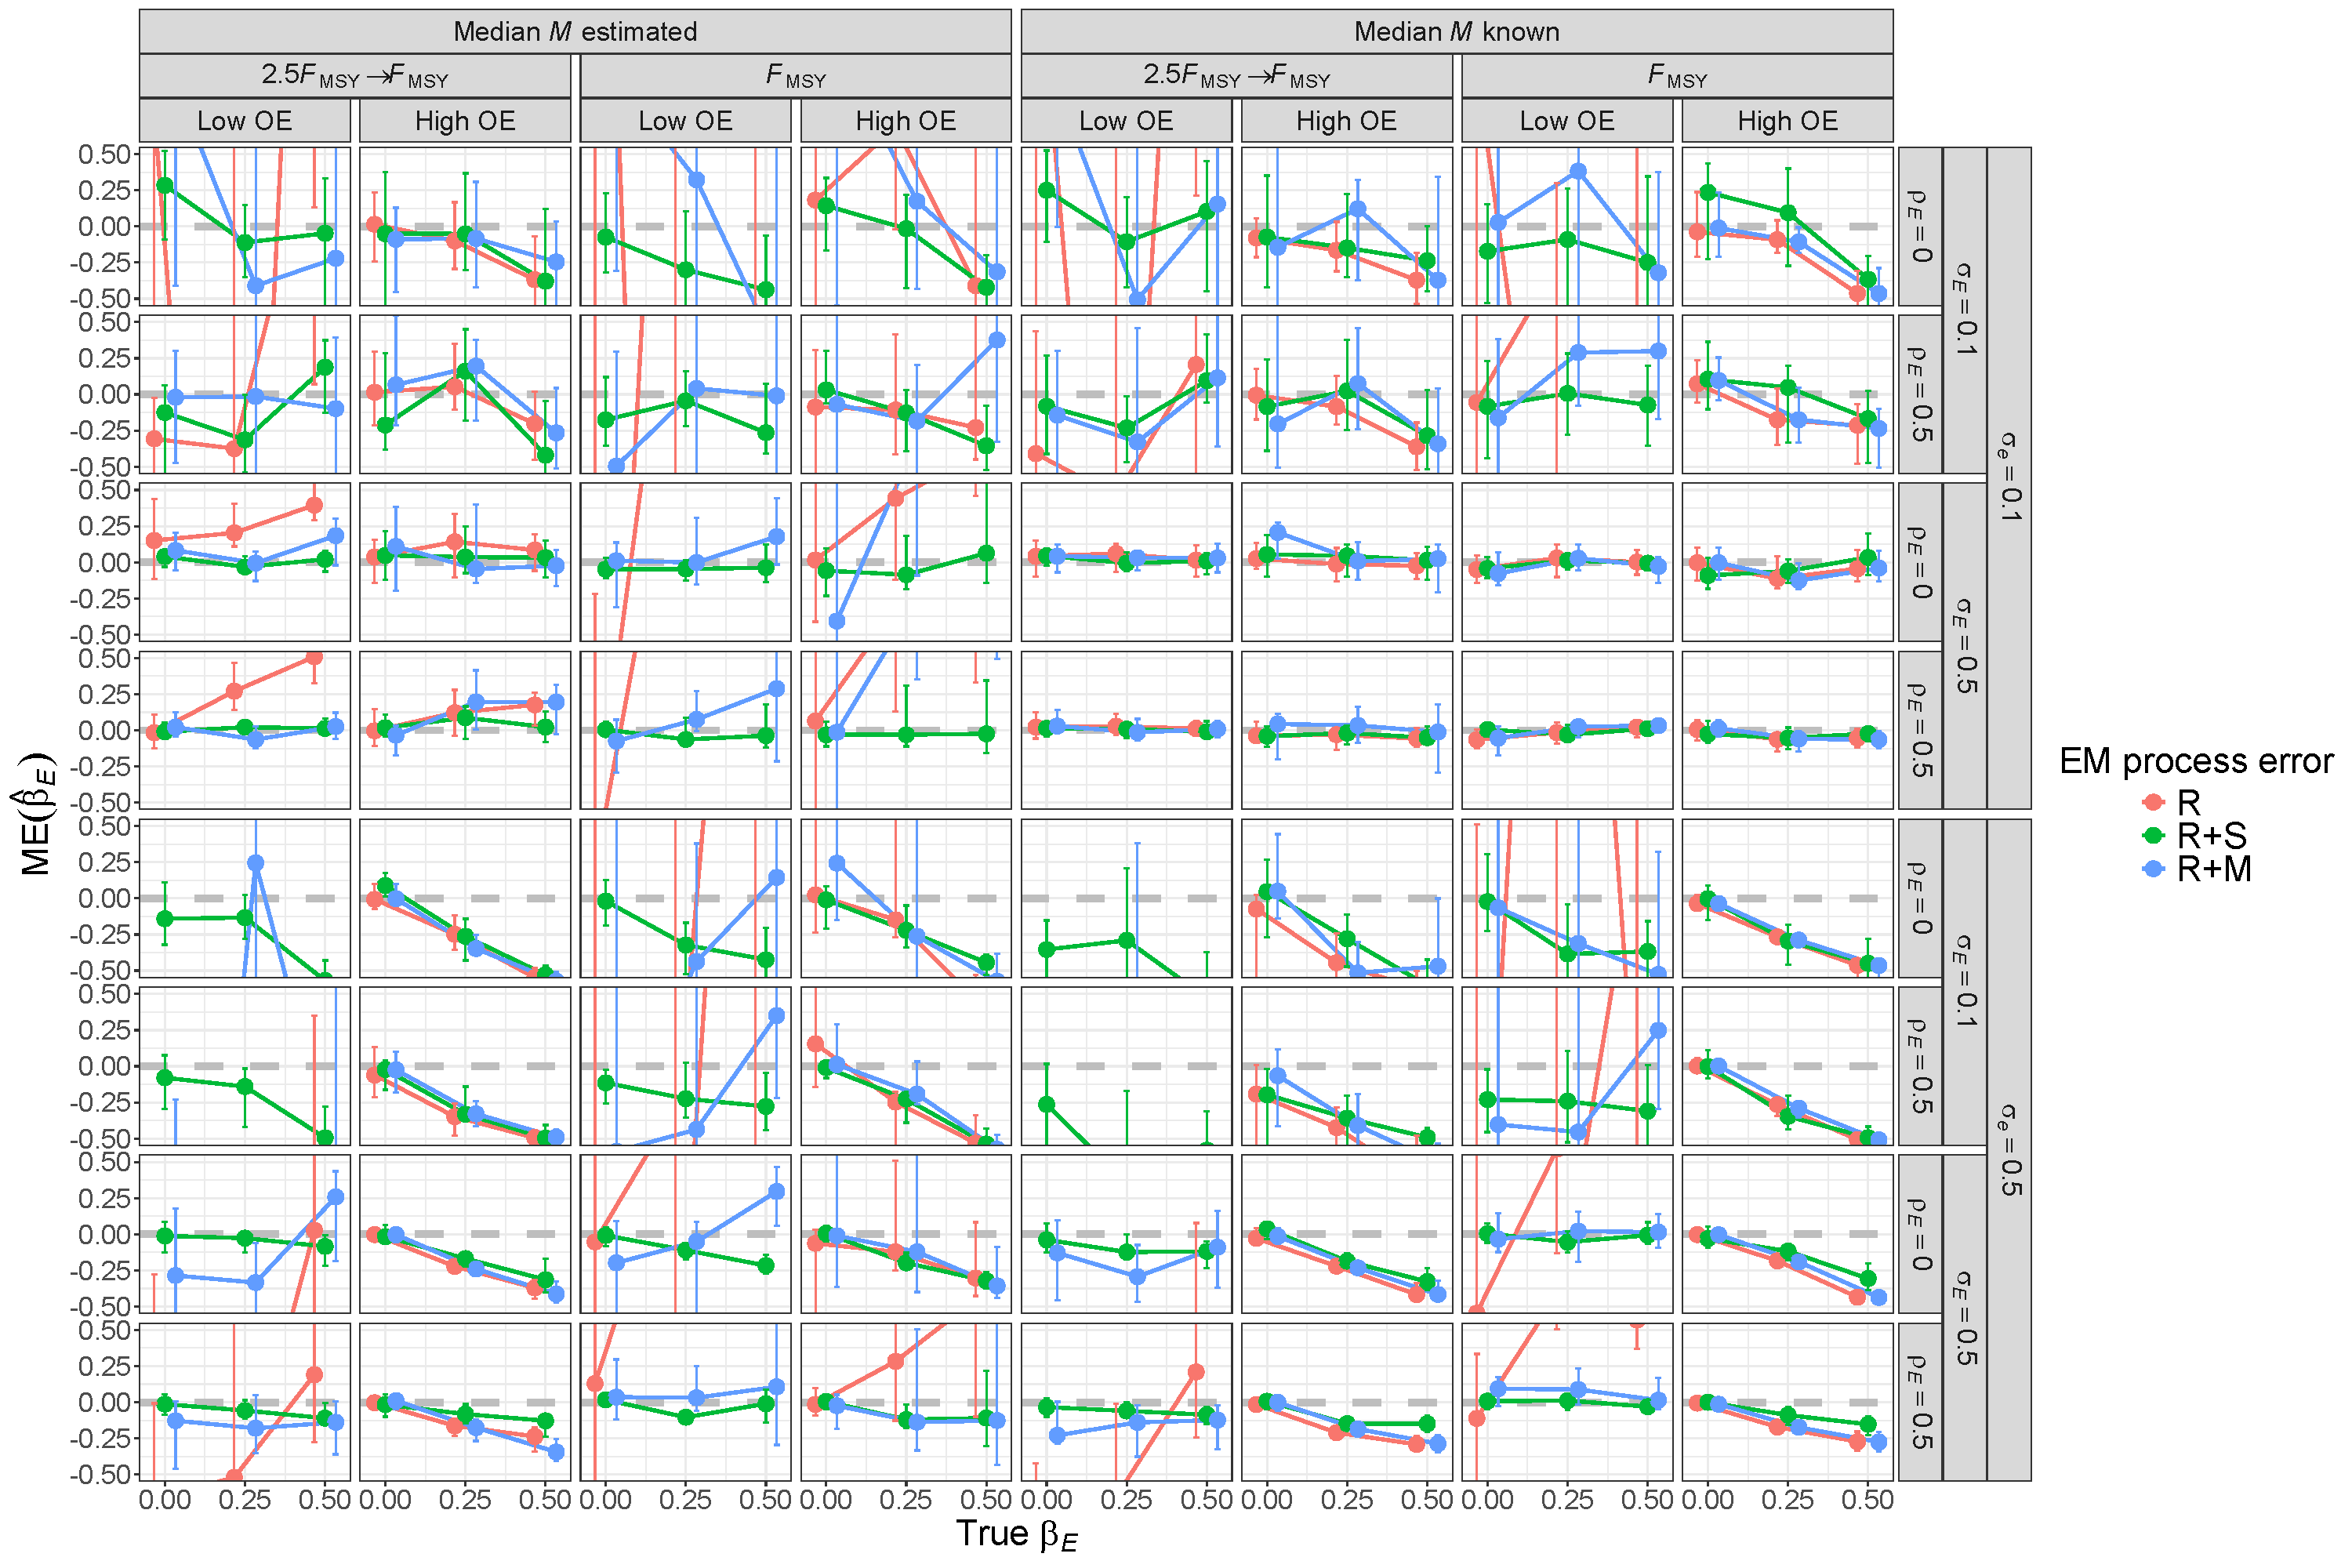
\includegraphics[height = \textheight]{beta_E_bias_RSom}
\end{center}
\caption{For R+S operating models, median error (ME) of estimates of environmental effect on $M$ ($\beta_E$) from fitting estimating models with alternative process error assumptions and treatment of median $M$ parameter ($\beta_M$). Vertical lines represent 95\% confidence intervals.}\label{beta_E_bias_RSom}
\end{figure}
\end{landscape}

\begin{landscape}
\begin{figure}
\begin{center}
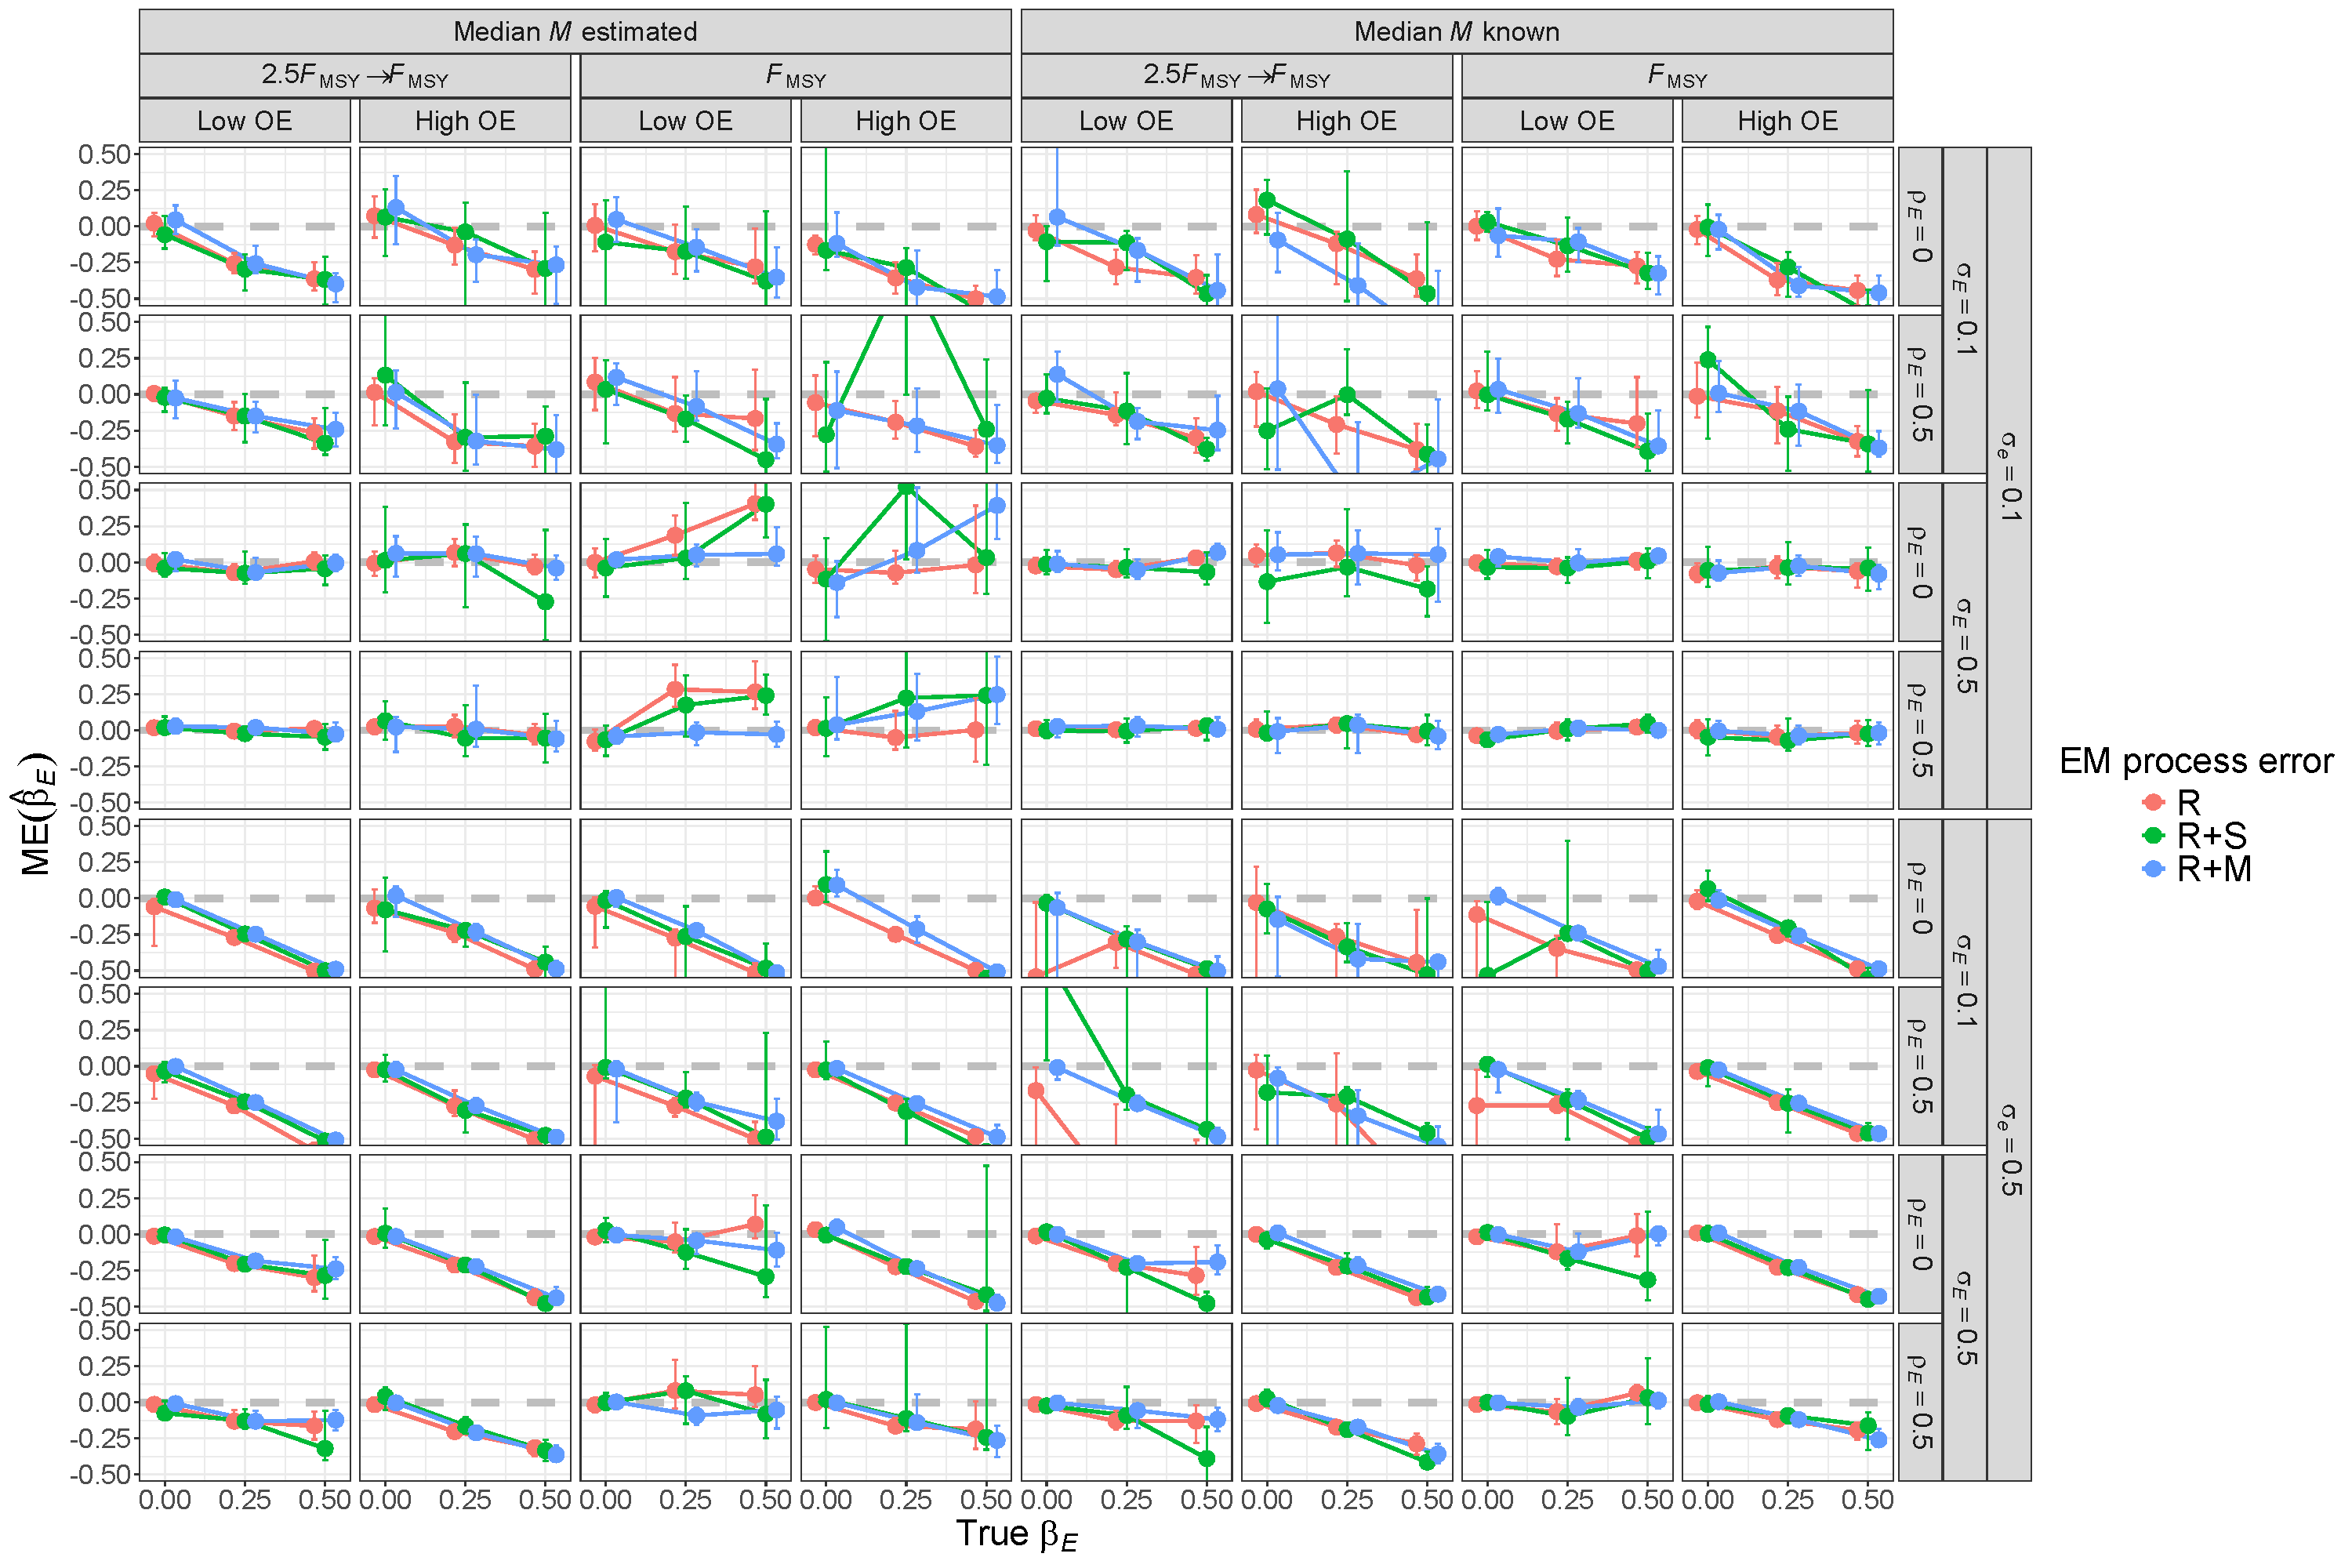
\includegraphics[height = \textheight]{beta_E_bias_RMom}
\end{center}
\caption{For R+M operating models, median error (ME) of estimates of environmental effect on $M$ ($\beta_E$) from fitting estimating models with alternative process error assumptions and treatment of median $M$ parameter ($\beta_M$). Vertical lines represent 95\% confidence intervals.}\label{beta_E_bias_RMom}
\end{figure}
\end{landscape}

\begin{landscape}
\begin{figure}
\begin{center}
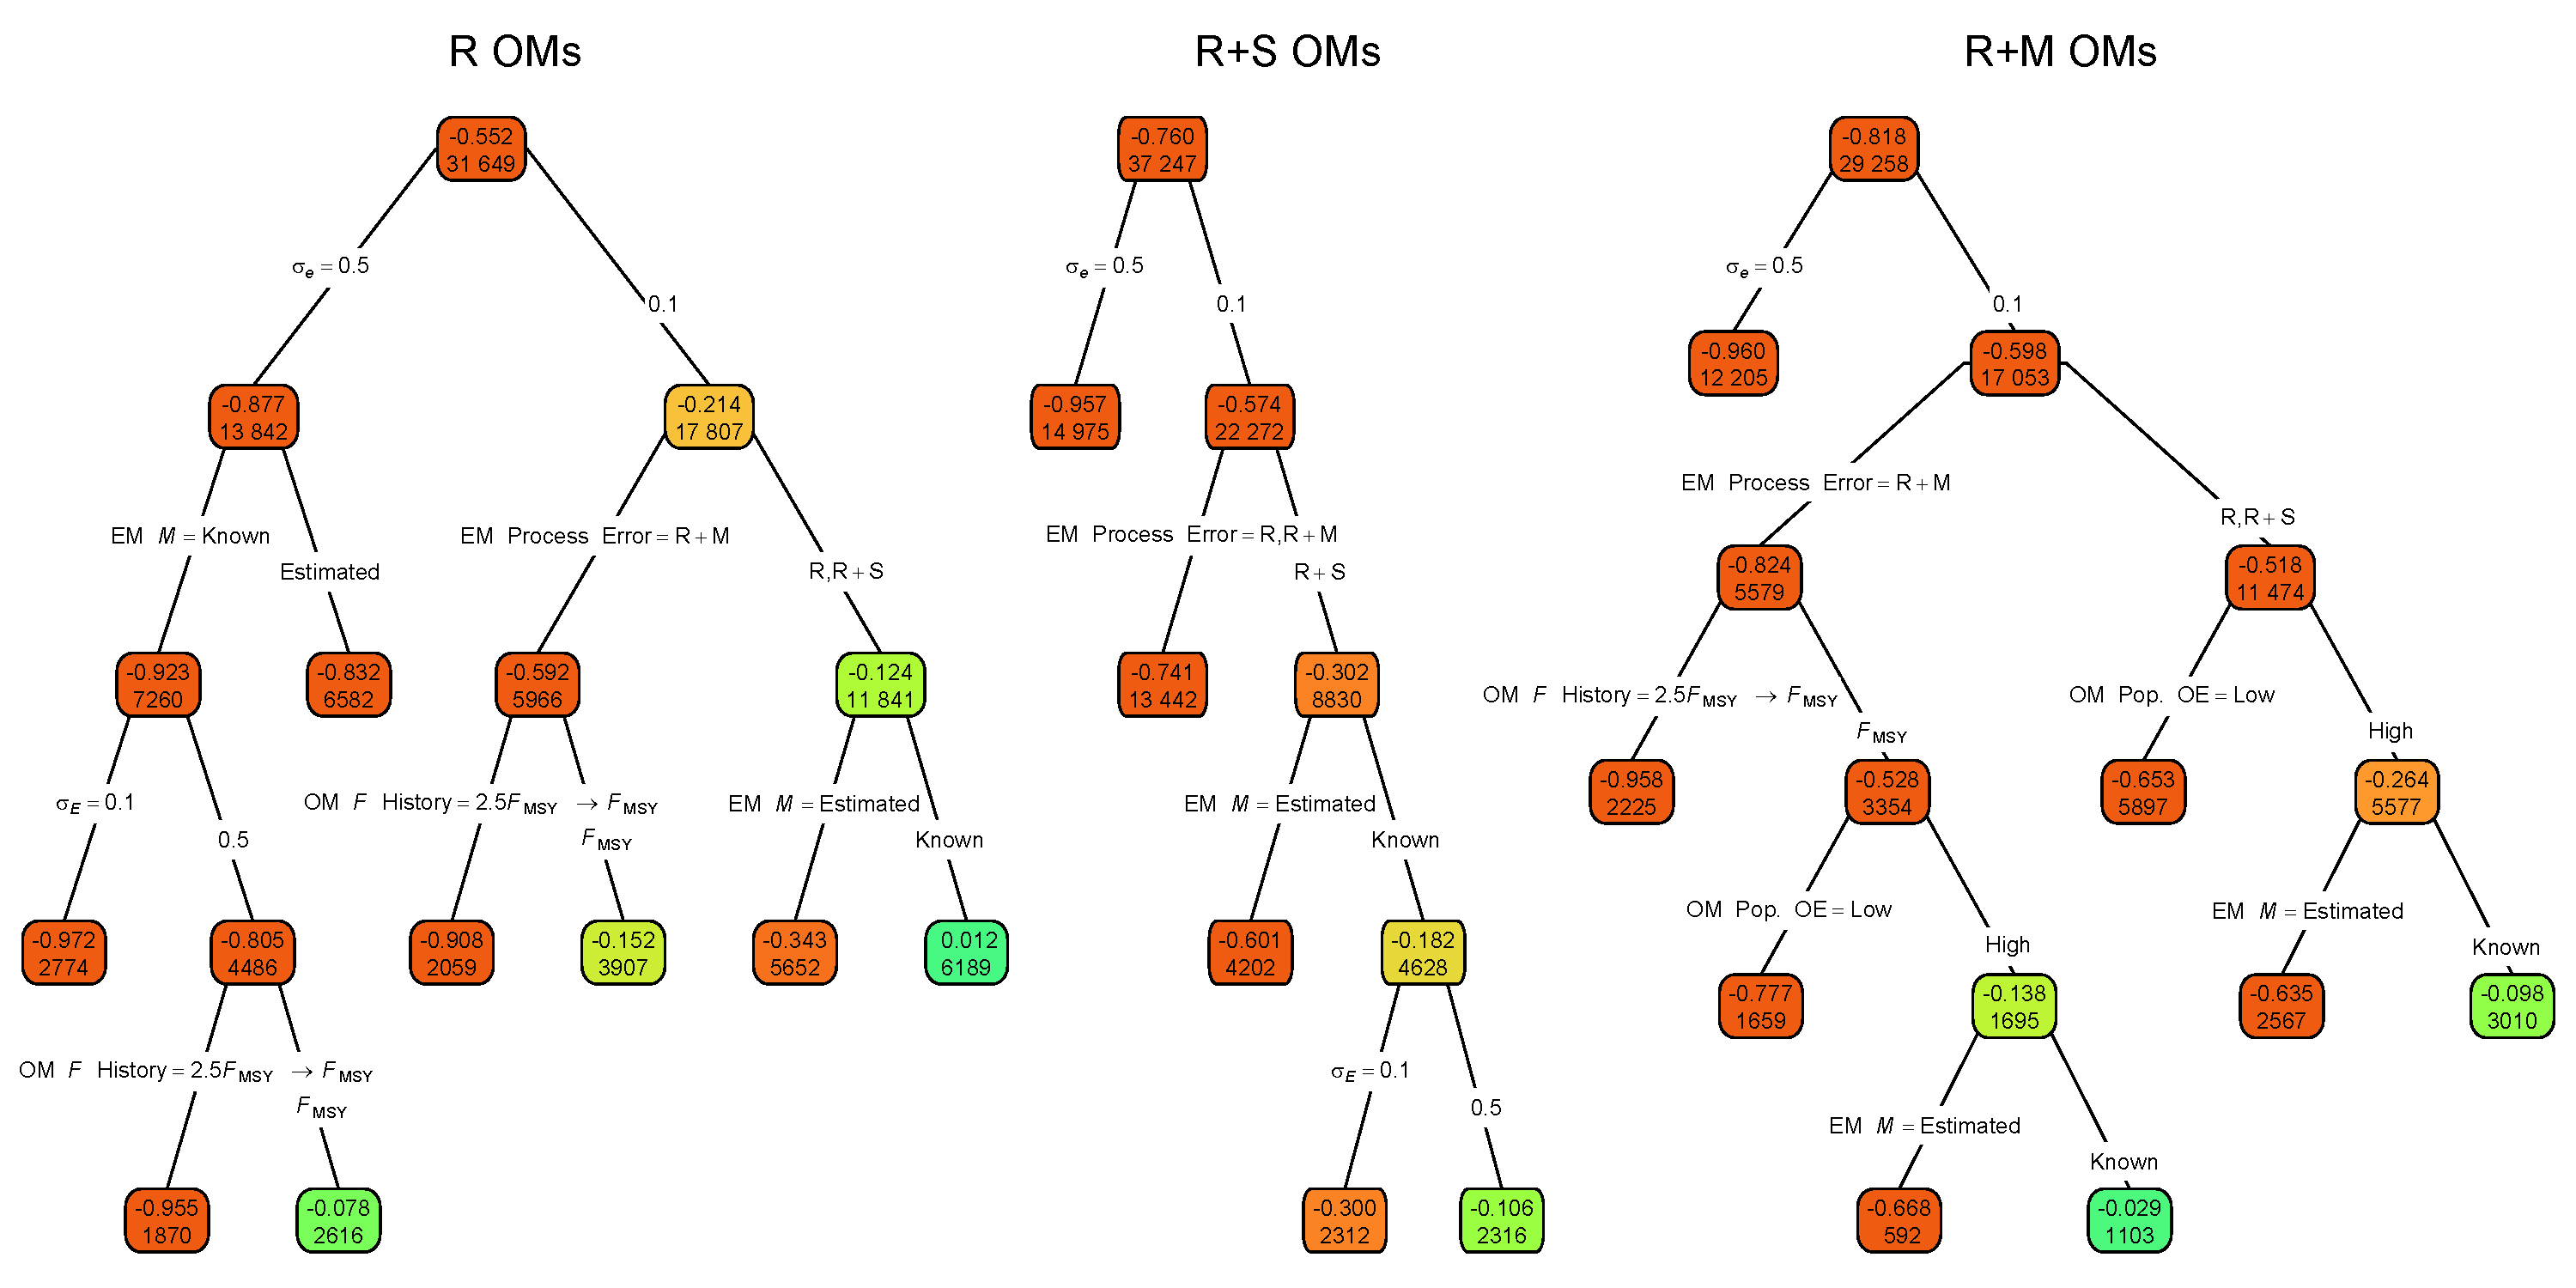
\includegraphics[width = 1.4\textwidth]{ecov_beta_SE_bias_regtree_plots}
\end{center}
\caption{Regression trees for error of the Hessian-based standard error estimates for covariate effect on $M$ ($\widehat {\text{SE}}\left(\widehat \beta_E\right)$). Each node shows the median error for the corresponding subset. Lower or higher absolute median errors are indicated by more green or red polygons, respectively. See Figure 1 caption and Table \ref{factor_table} for further details.}\label{ecov_effect_SE_bias_regtree}
\end{figure}
\end{landscape}

\begin{landscape}
\begin{figure}
\begin{center}
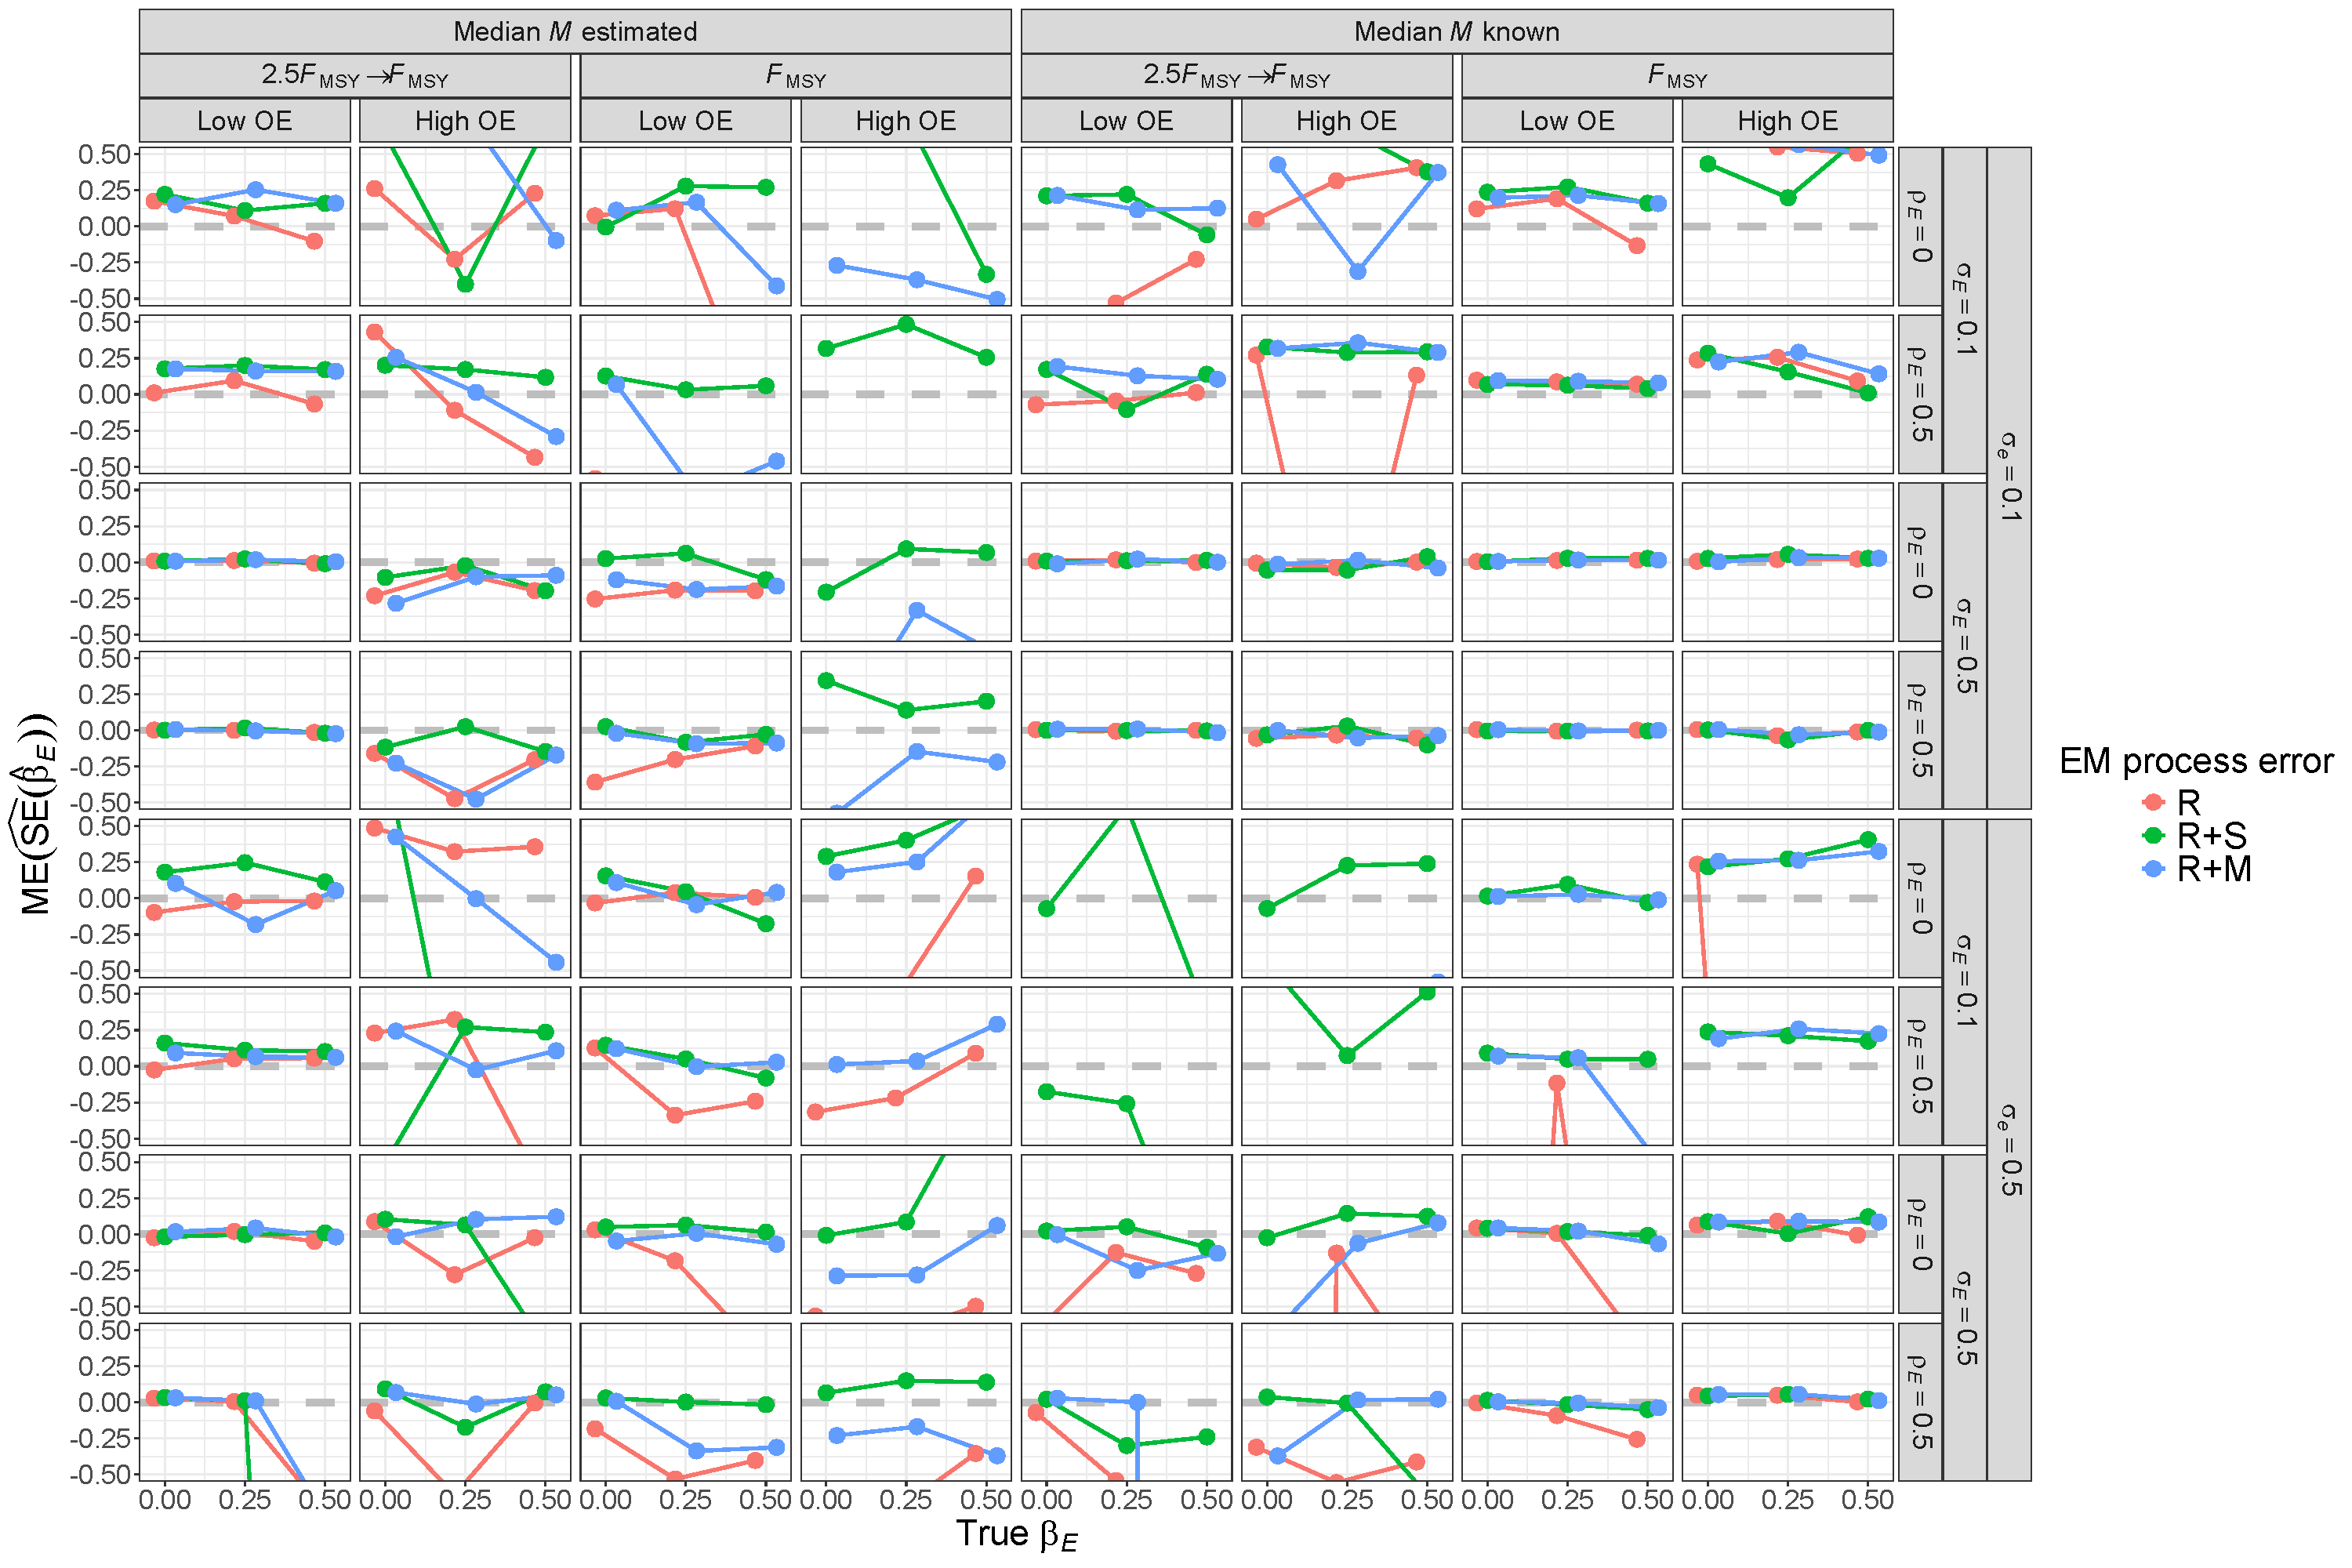
\includegraphics[height = \textheight]{se_beta_E_bias_Rom}
\end{center}
\caption{For R operating models, median error (ME) of Hessian-based estimates of standard error for covariate effect on $M$ ($\beta_E$) from fitting estimating models with alternative process error assumptions and treatment of median $M$ parameter ($\beta_M$). True standard error is defined as the mean of the standard error estimates accross converged fits to simulated data sets for a given operating model scenario.}\label{se_beta_E_bias_Rom}
\end{figure}
\end{landscape}

\begin{landscape}
\begin{figure}
\begin{center}
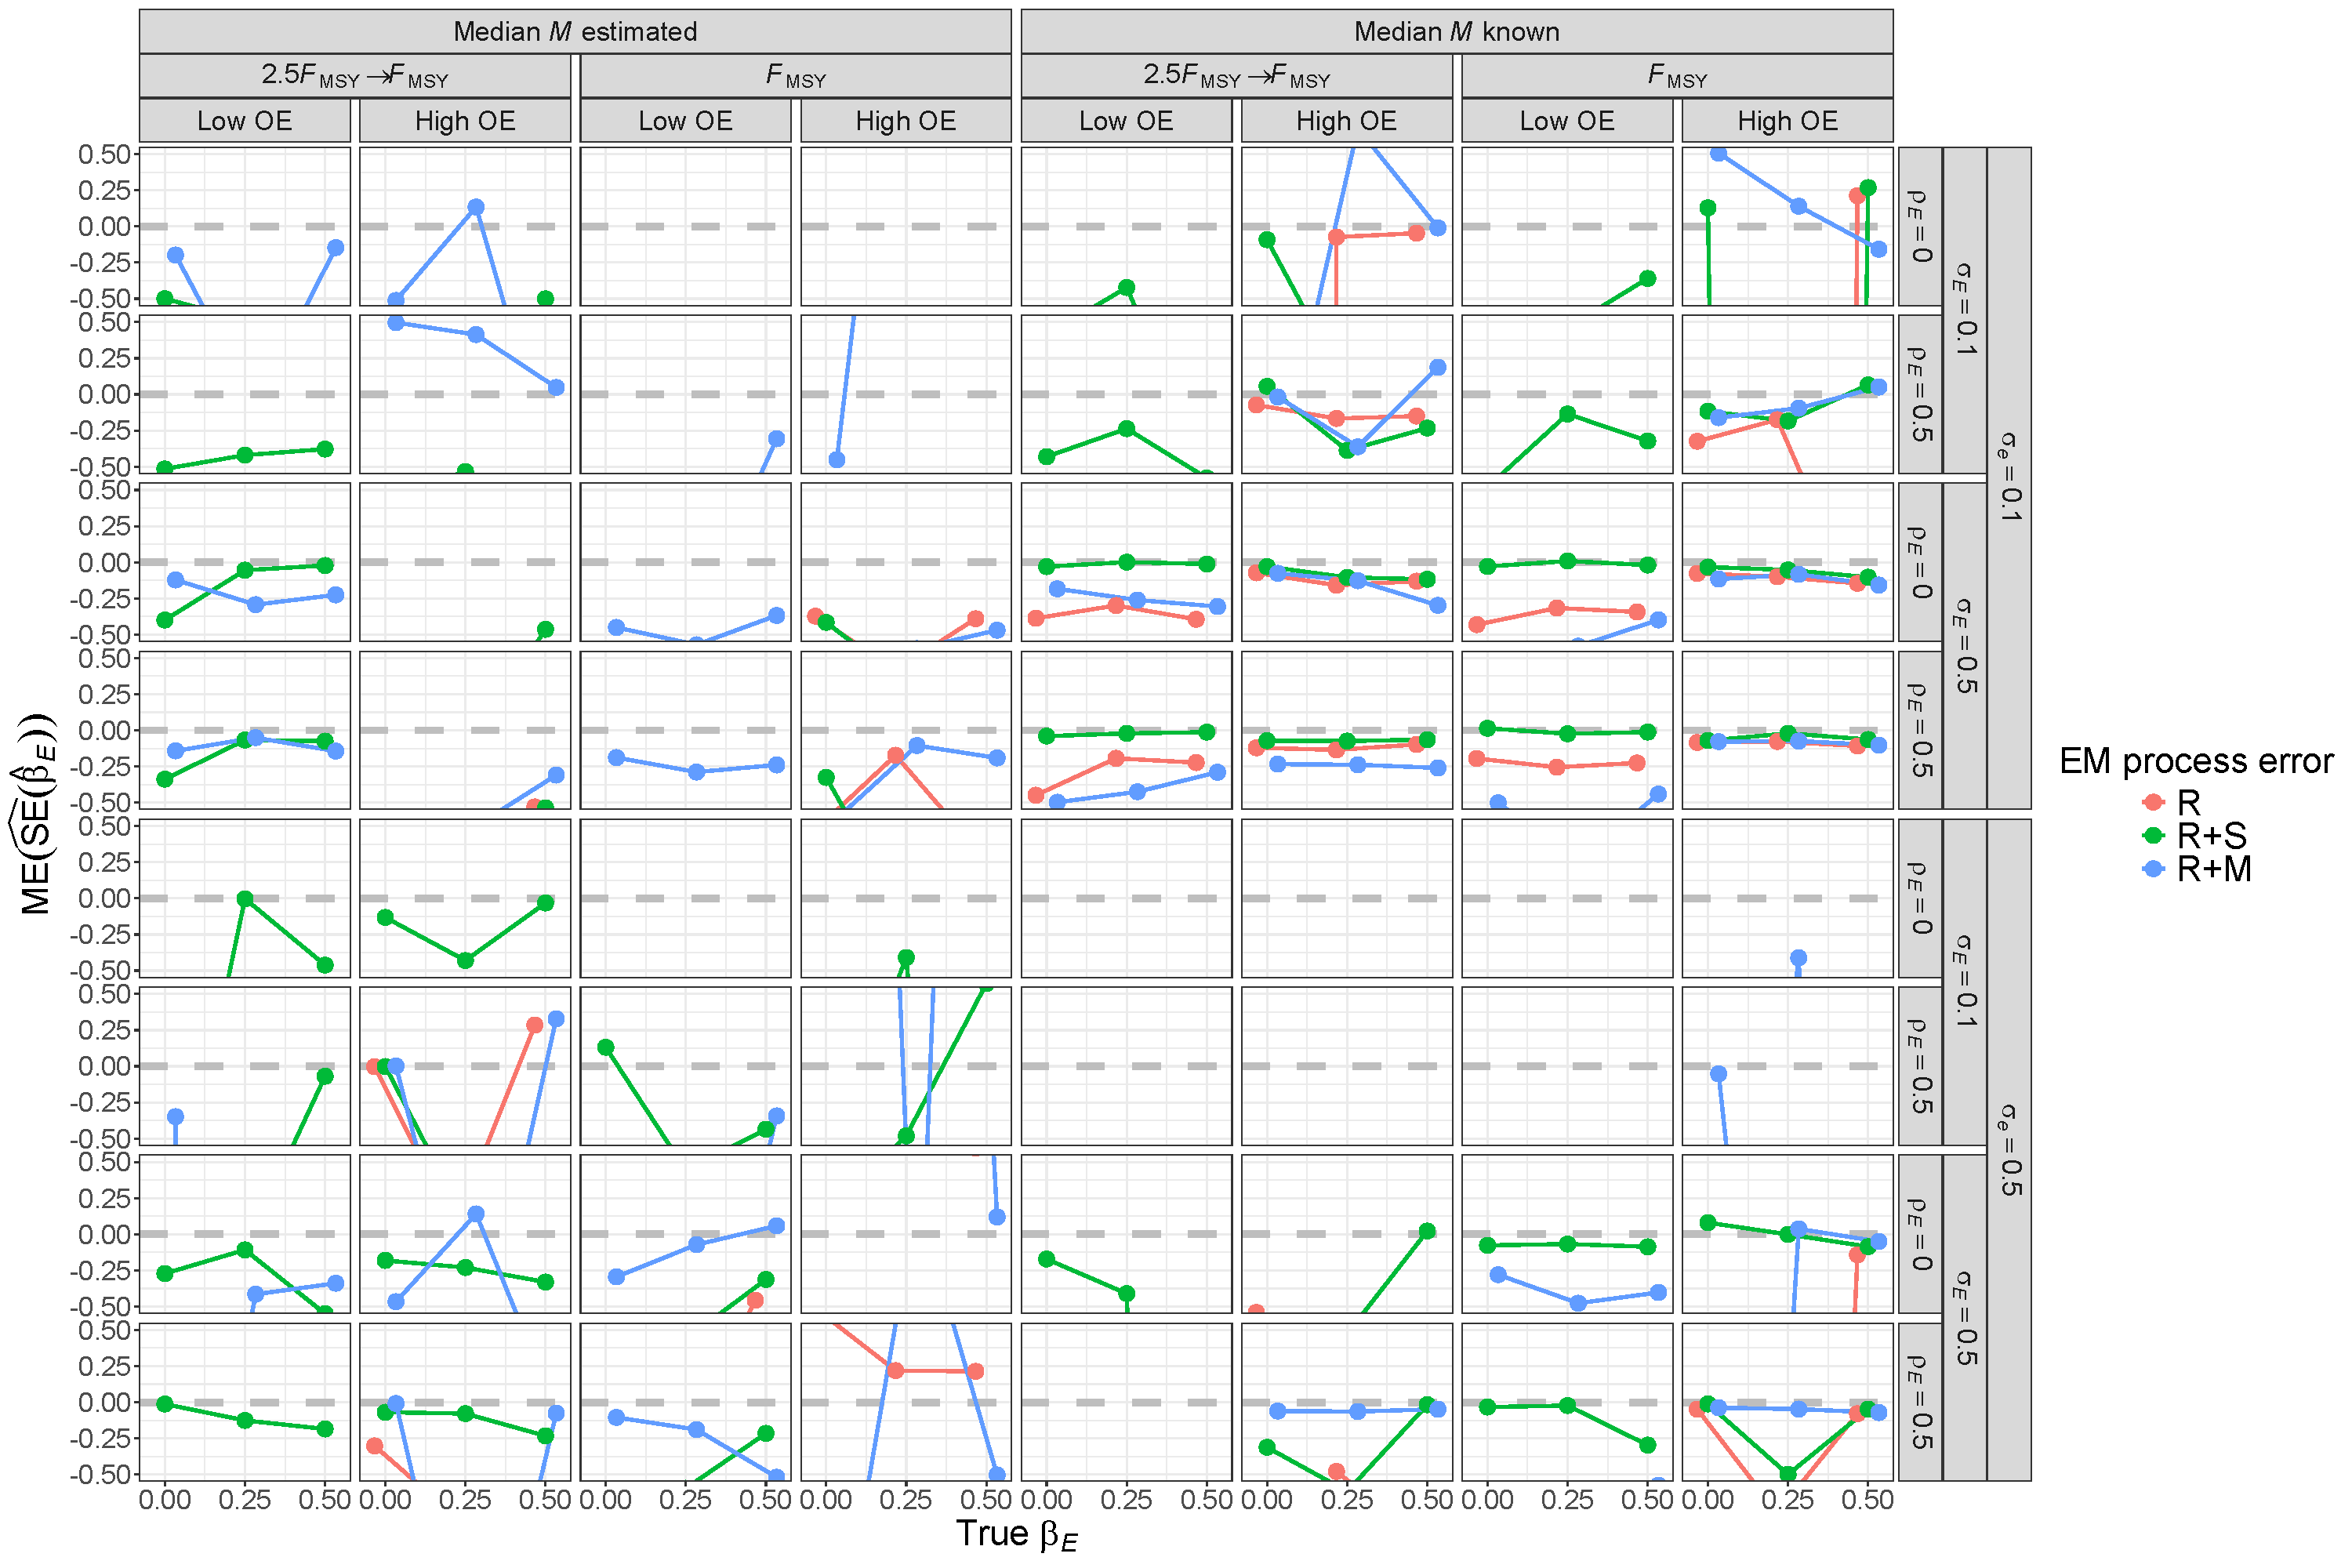
\includegraphics[height = \textheight]{se_beta_E_bias_RSom}
\end{center}
\caption{For R+S operating models, median error (ME) of Hessian-based estimates of standard error for covariate effect on $M$ ($\beta_E$) from fitting estimating models with alternative process error assumptions and treatment of median $M$ parameter ($\beta_M$). True standard error is defined as the mean of the standard error estimates accross converged fits to simulated data sets for a given operating model scenario.}\label{se_beta_E_bias_RSom}
\end{figure}
\end{landscape}

\begin{landscape}
\begin{figure}
\begin{center}
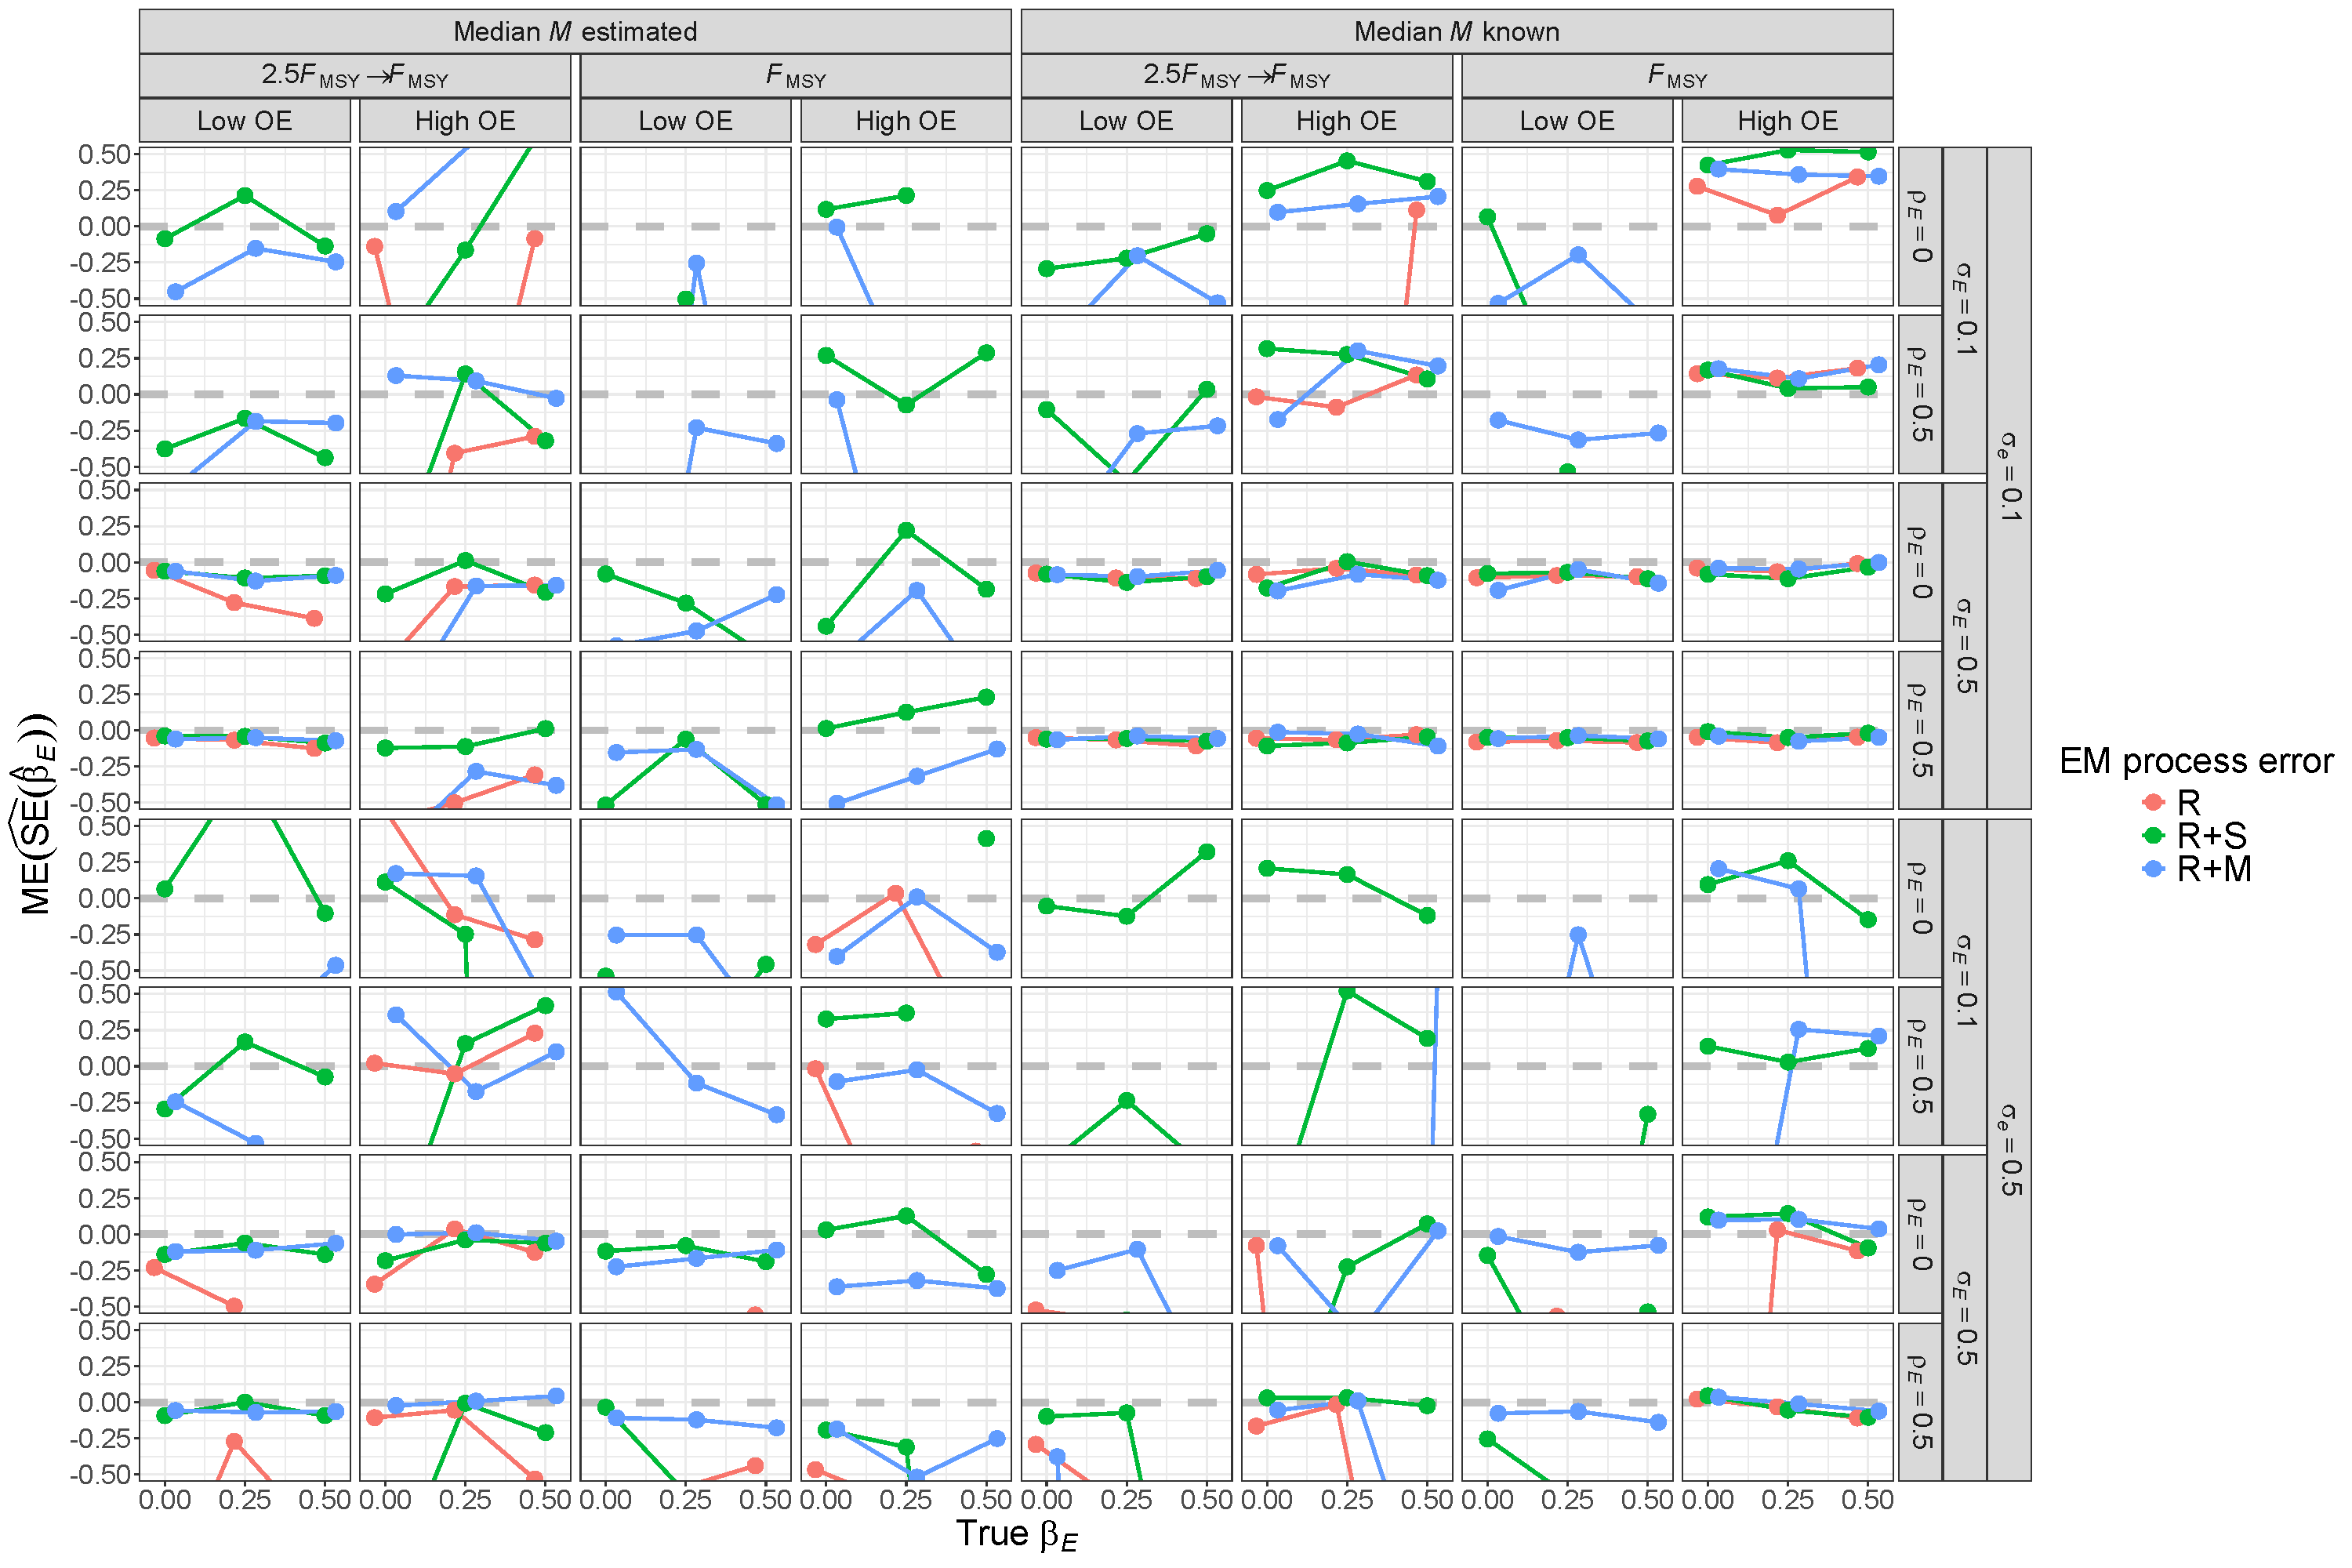
\includegraphics[height = \textheight]{se_beta_E_bias_RMom}
\end{center}
\caption{For R+M operating models, median error (ME) of Hessian-based estimates of standard error for covariate effect on $M$ ($\beta_E$) from fitting estimating models with alternative process error assumptions and treatment of median $M$ parameter ($\beta_M$). True standard error is defined as the mean of the standard error estimates accross converged fits to simulated data sets for a given operating model scenario.}\label{se_beta_E_bias_RMom}
\end{figure}
\end{landscape}

\begin{landscape}
\begin{figure}
\begin{center}
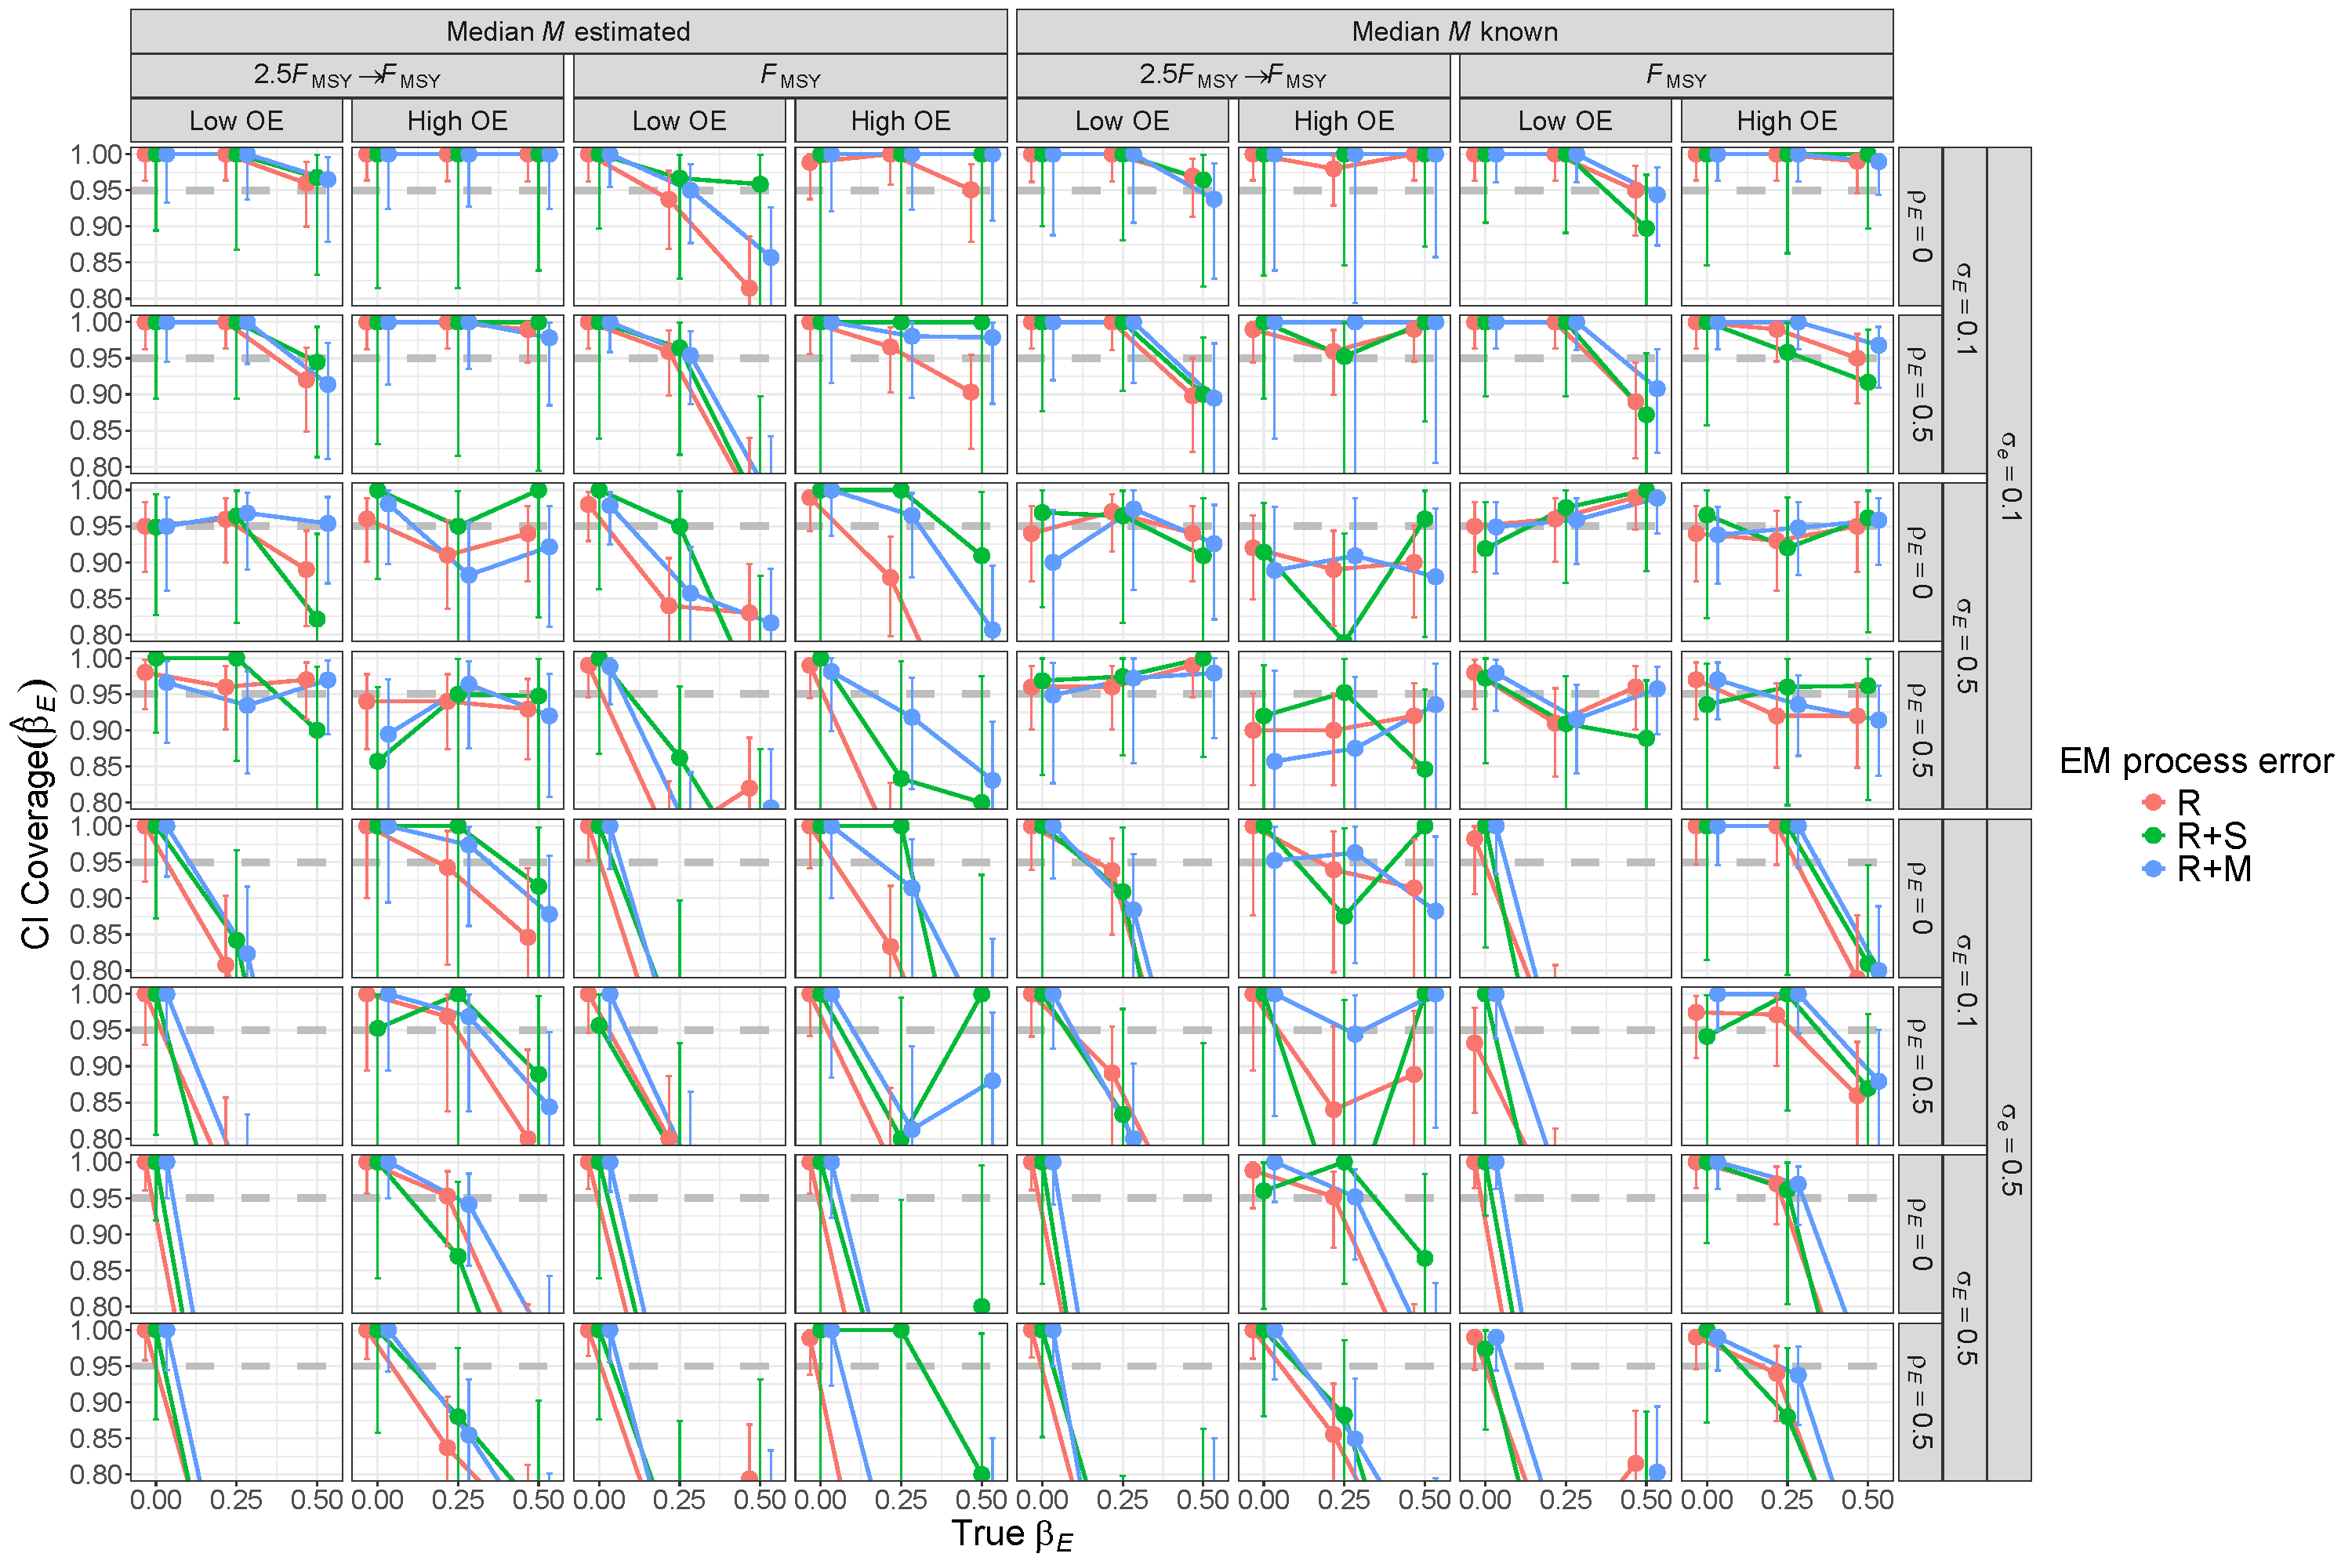
\includegraphics[height = \textheight]{beta_E_CI_coverage_Rom}
\end{center}
\caption{For R operating models, probability of 95\% confidence interval for $\beta_E$ containing the true value for estimating models with alternative process error assumptions and treatment of median $M$ parameter ($\beta_M$). Vertical lines represent 95\% confidence intervals.}\label{beta_E_CI_coverage_Rom}
\end{figure}
\end{landscape}

\begin{landscape}
\begin{figure}
\begin{center}
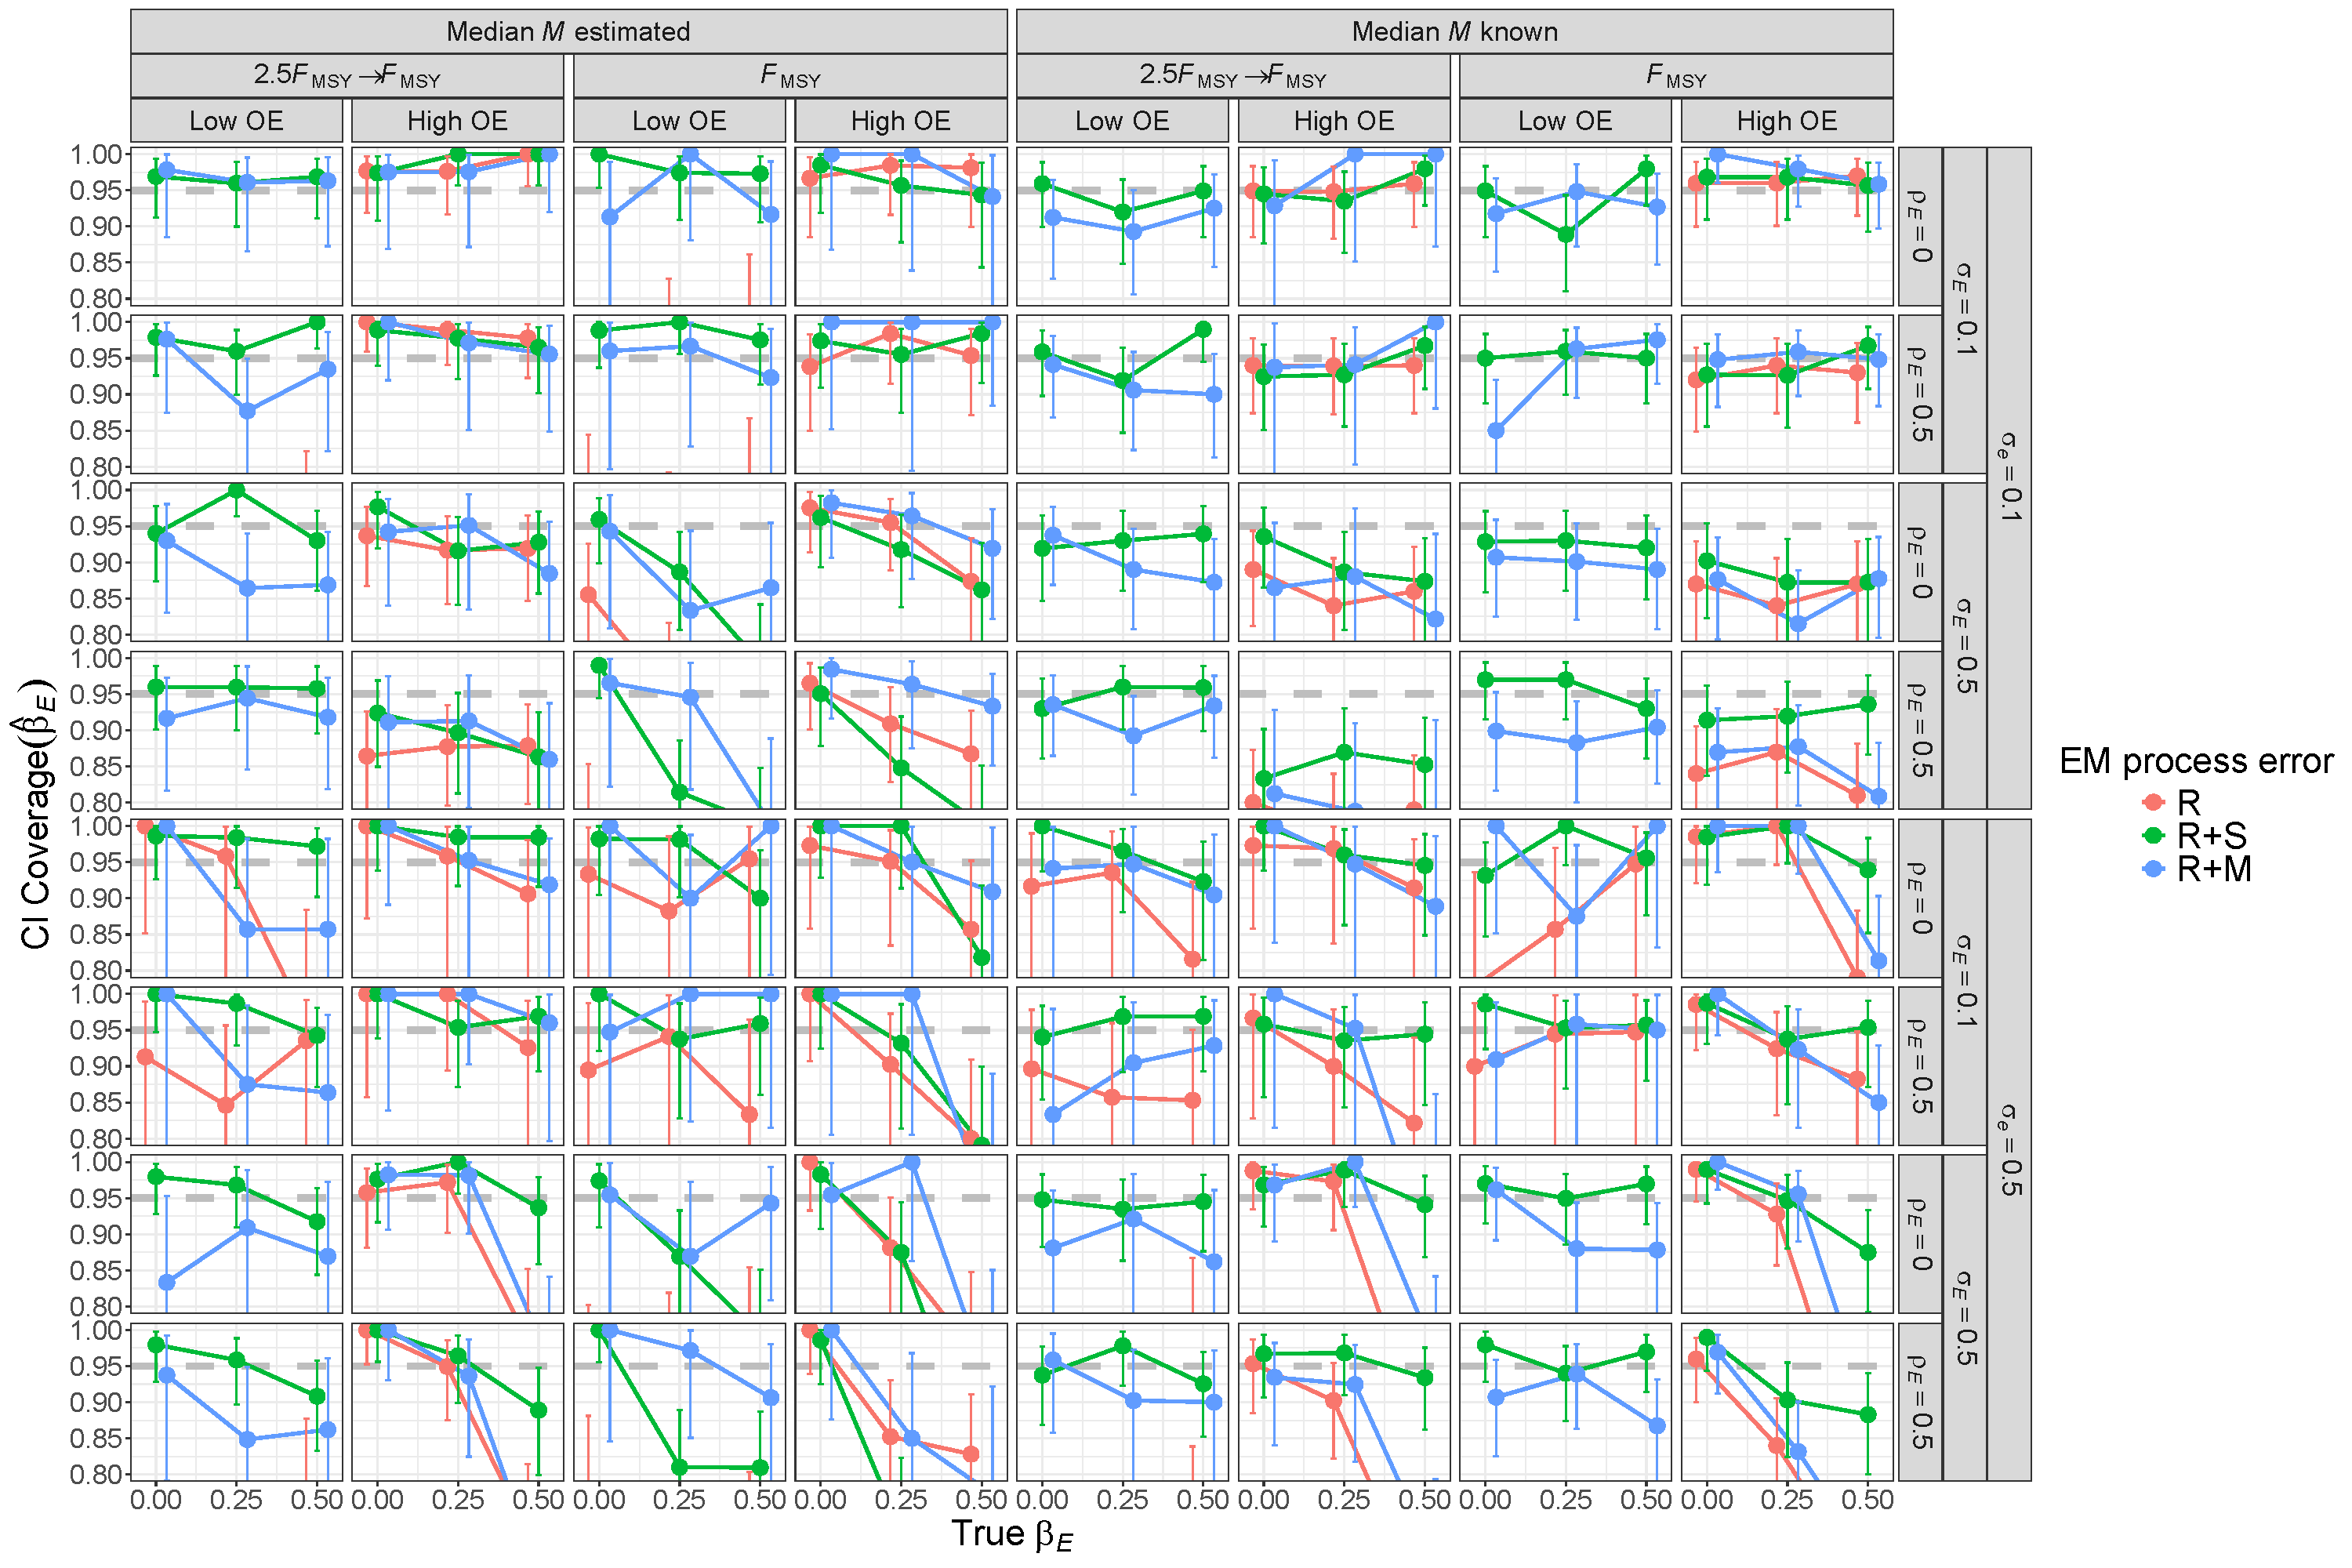
\includegraphics[height = \textheight]{beta_E_CI_coverage_RSom}
\end{center}
\caption{For R+S operating models, probability of 95\% confidence interval for $\beta_E$ containing the true value for estimating models with alternative process error assumptions and treatment of median $M$ parameter ($\beta_M$). Vertical lines represent 95\% confidence intervals.}\label{beta_E_CI_coverage_RSom}
\end{figure}
\end{landscape}

\begin{landscape}
\begin{figure}
\begin{center}
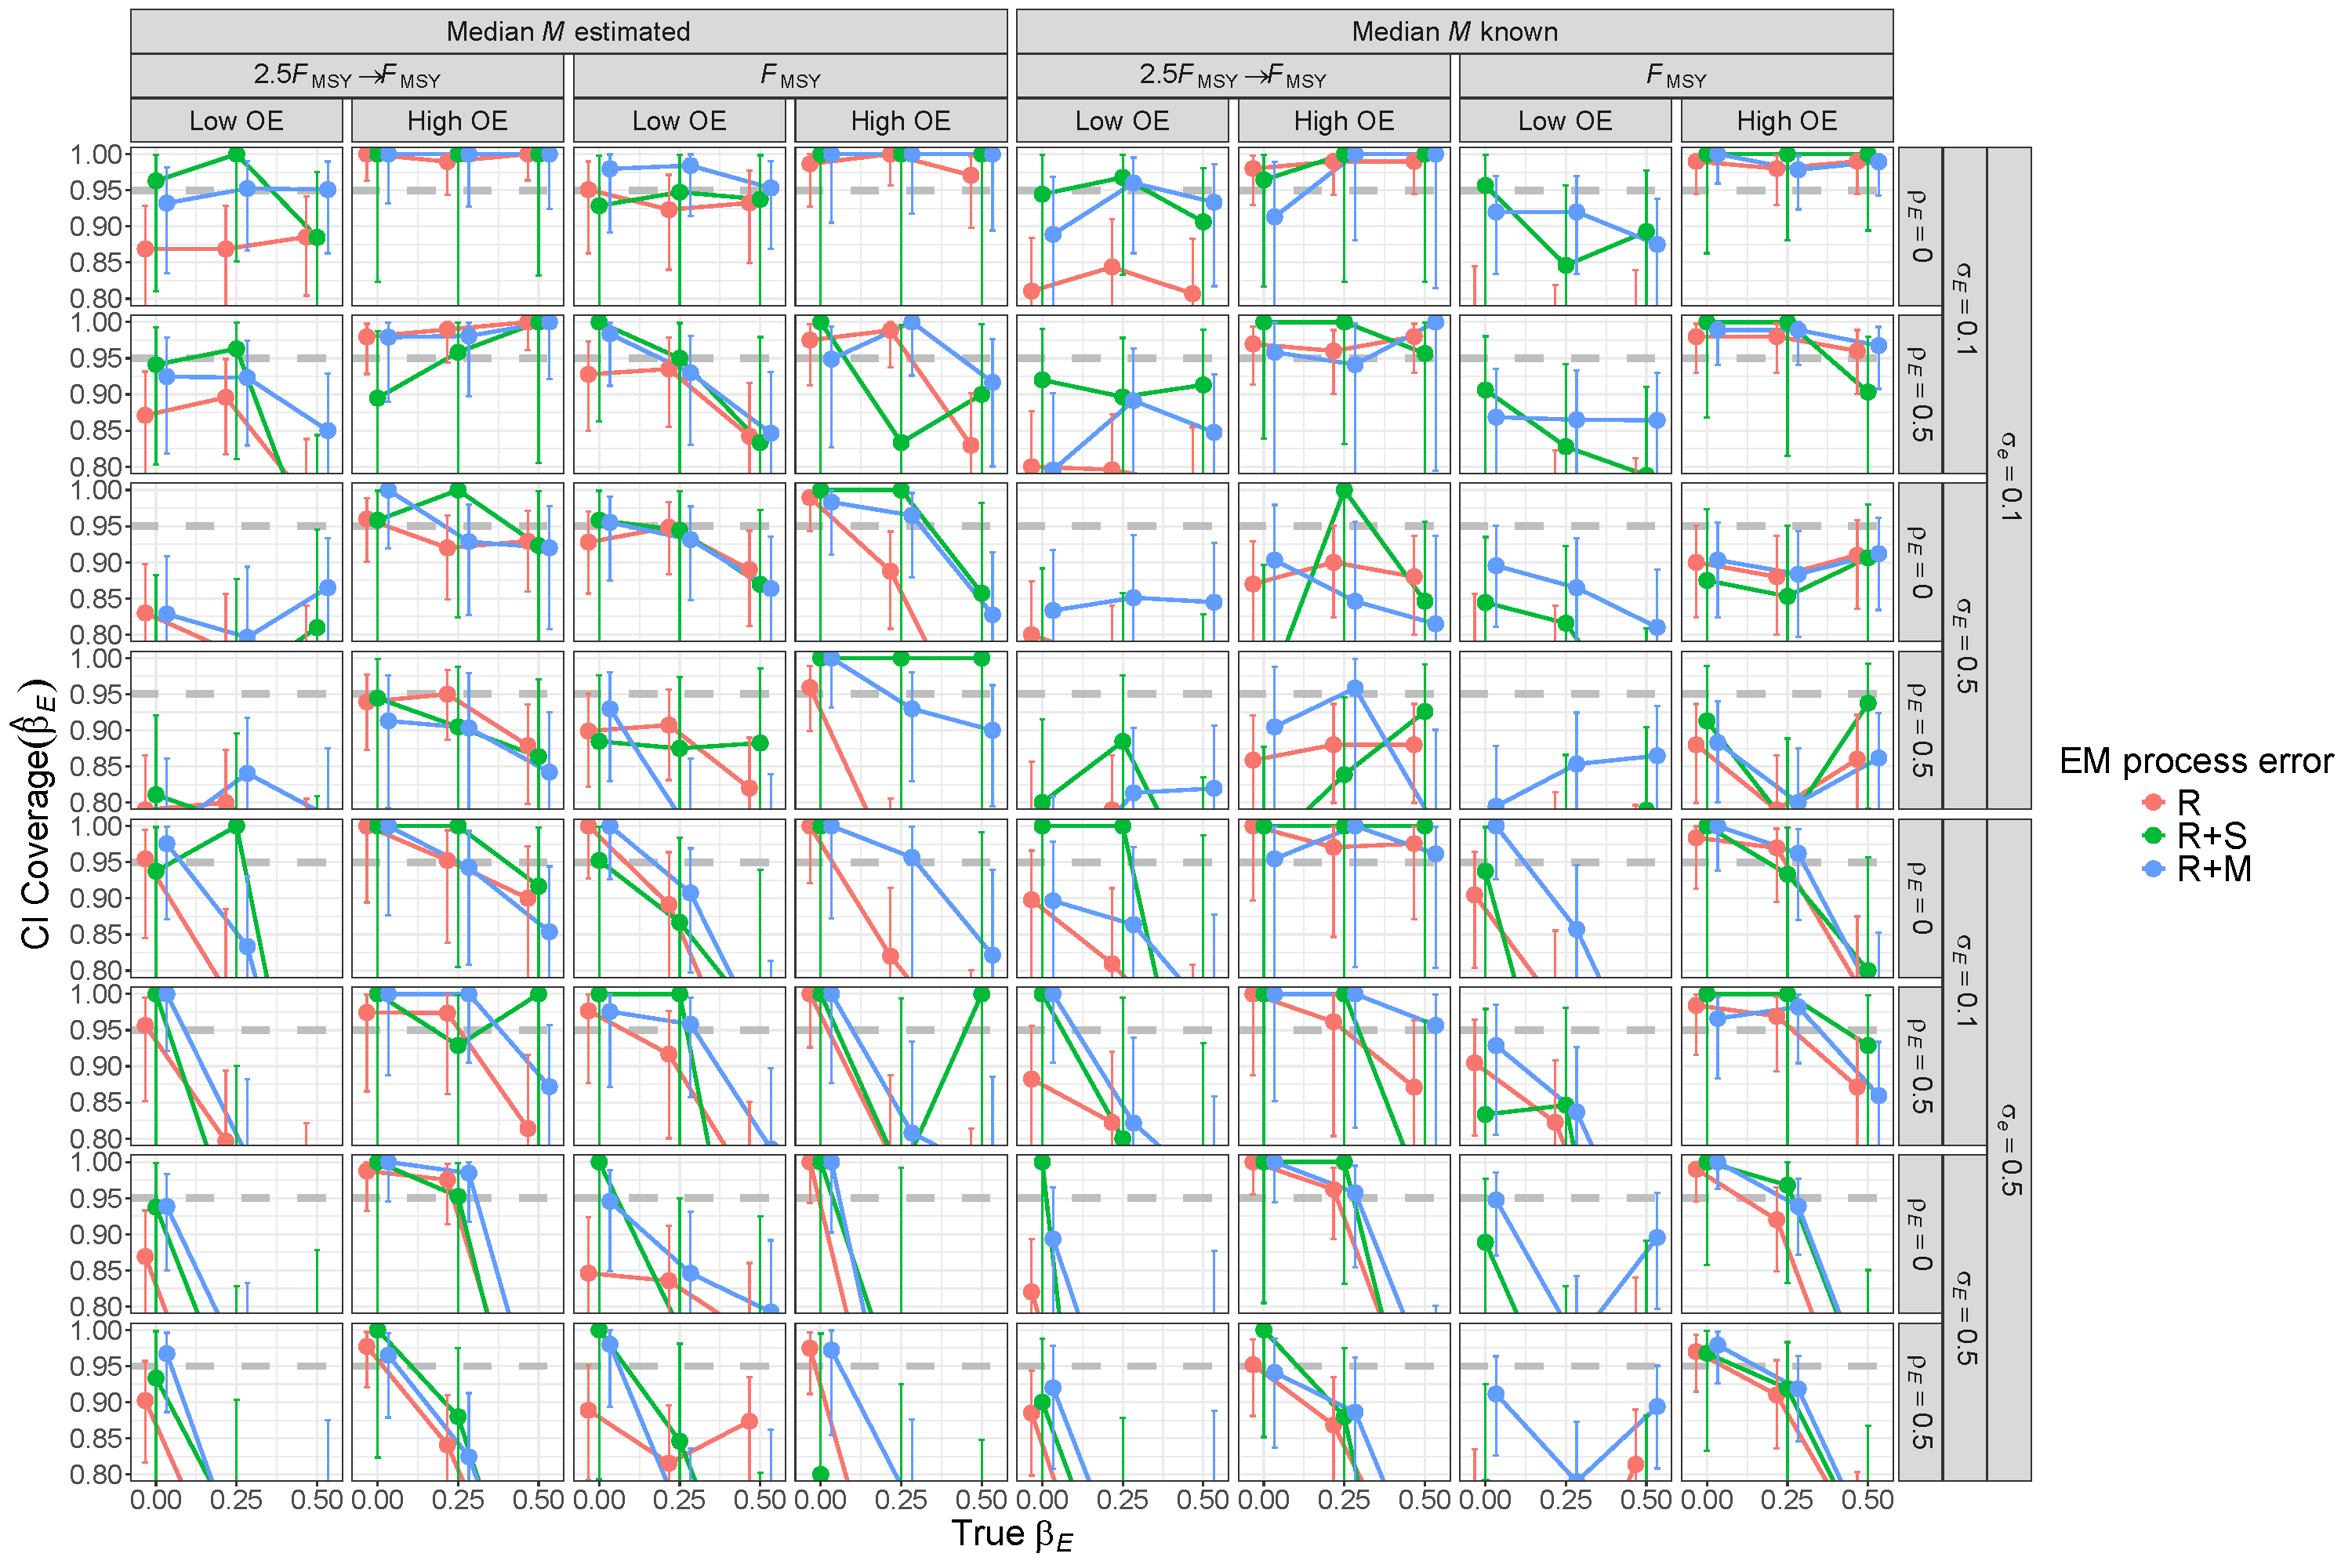
\includegraphics[height = \textheight]{beta_E_CI_coverage_RMom}
\end{center}
\caption{For R+M operating models, probability of 95\% confidence interval for $\beta_E$ containing the true value for estimating models with alternative process error assumptions and treatment of median $M$ parameter ($\beta_M$). Vertical lines represent 95\% confidence intervals.}\label{beta_E_CI_coverage_RMom}
\end{figure}
\end{landscape}

\begin{landscape}
\begin{figure}
\begin{center}
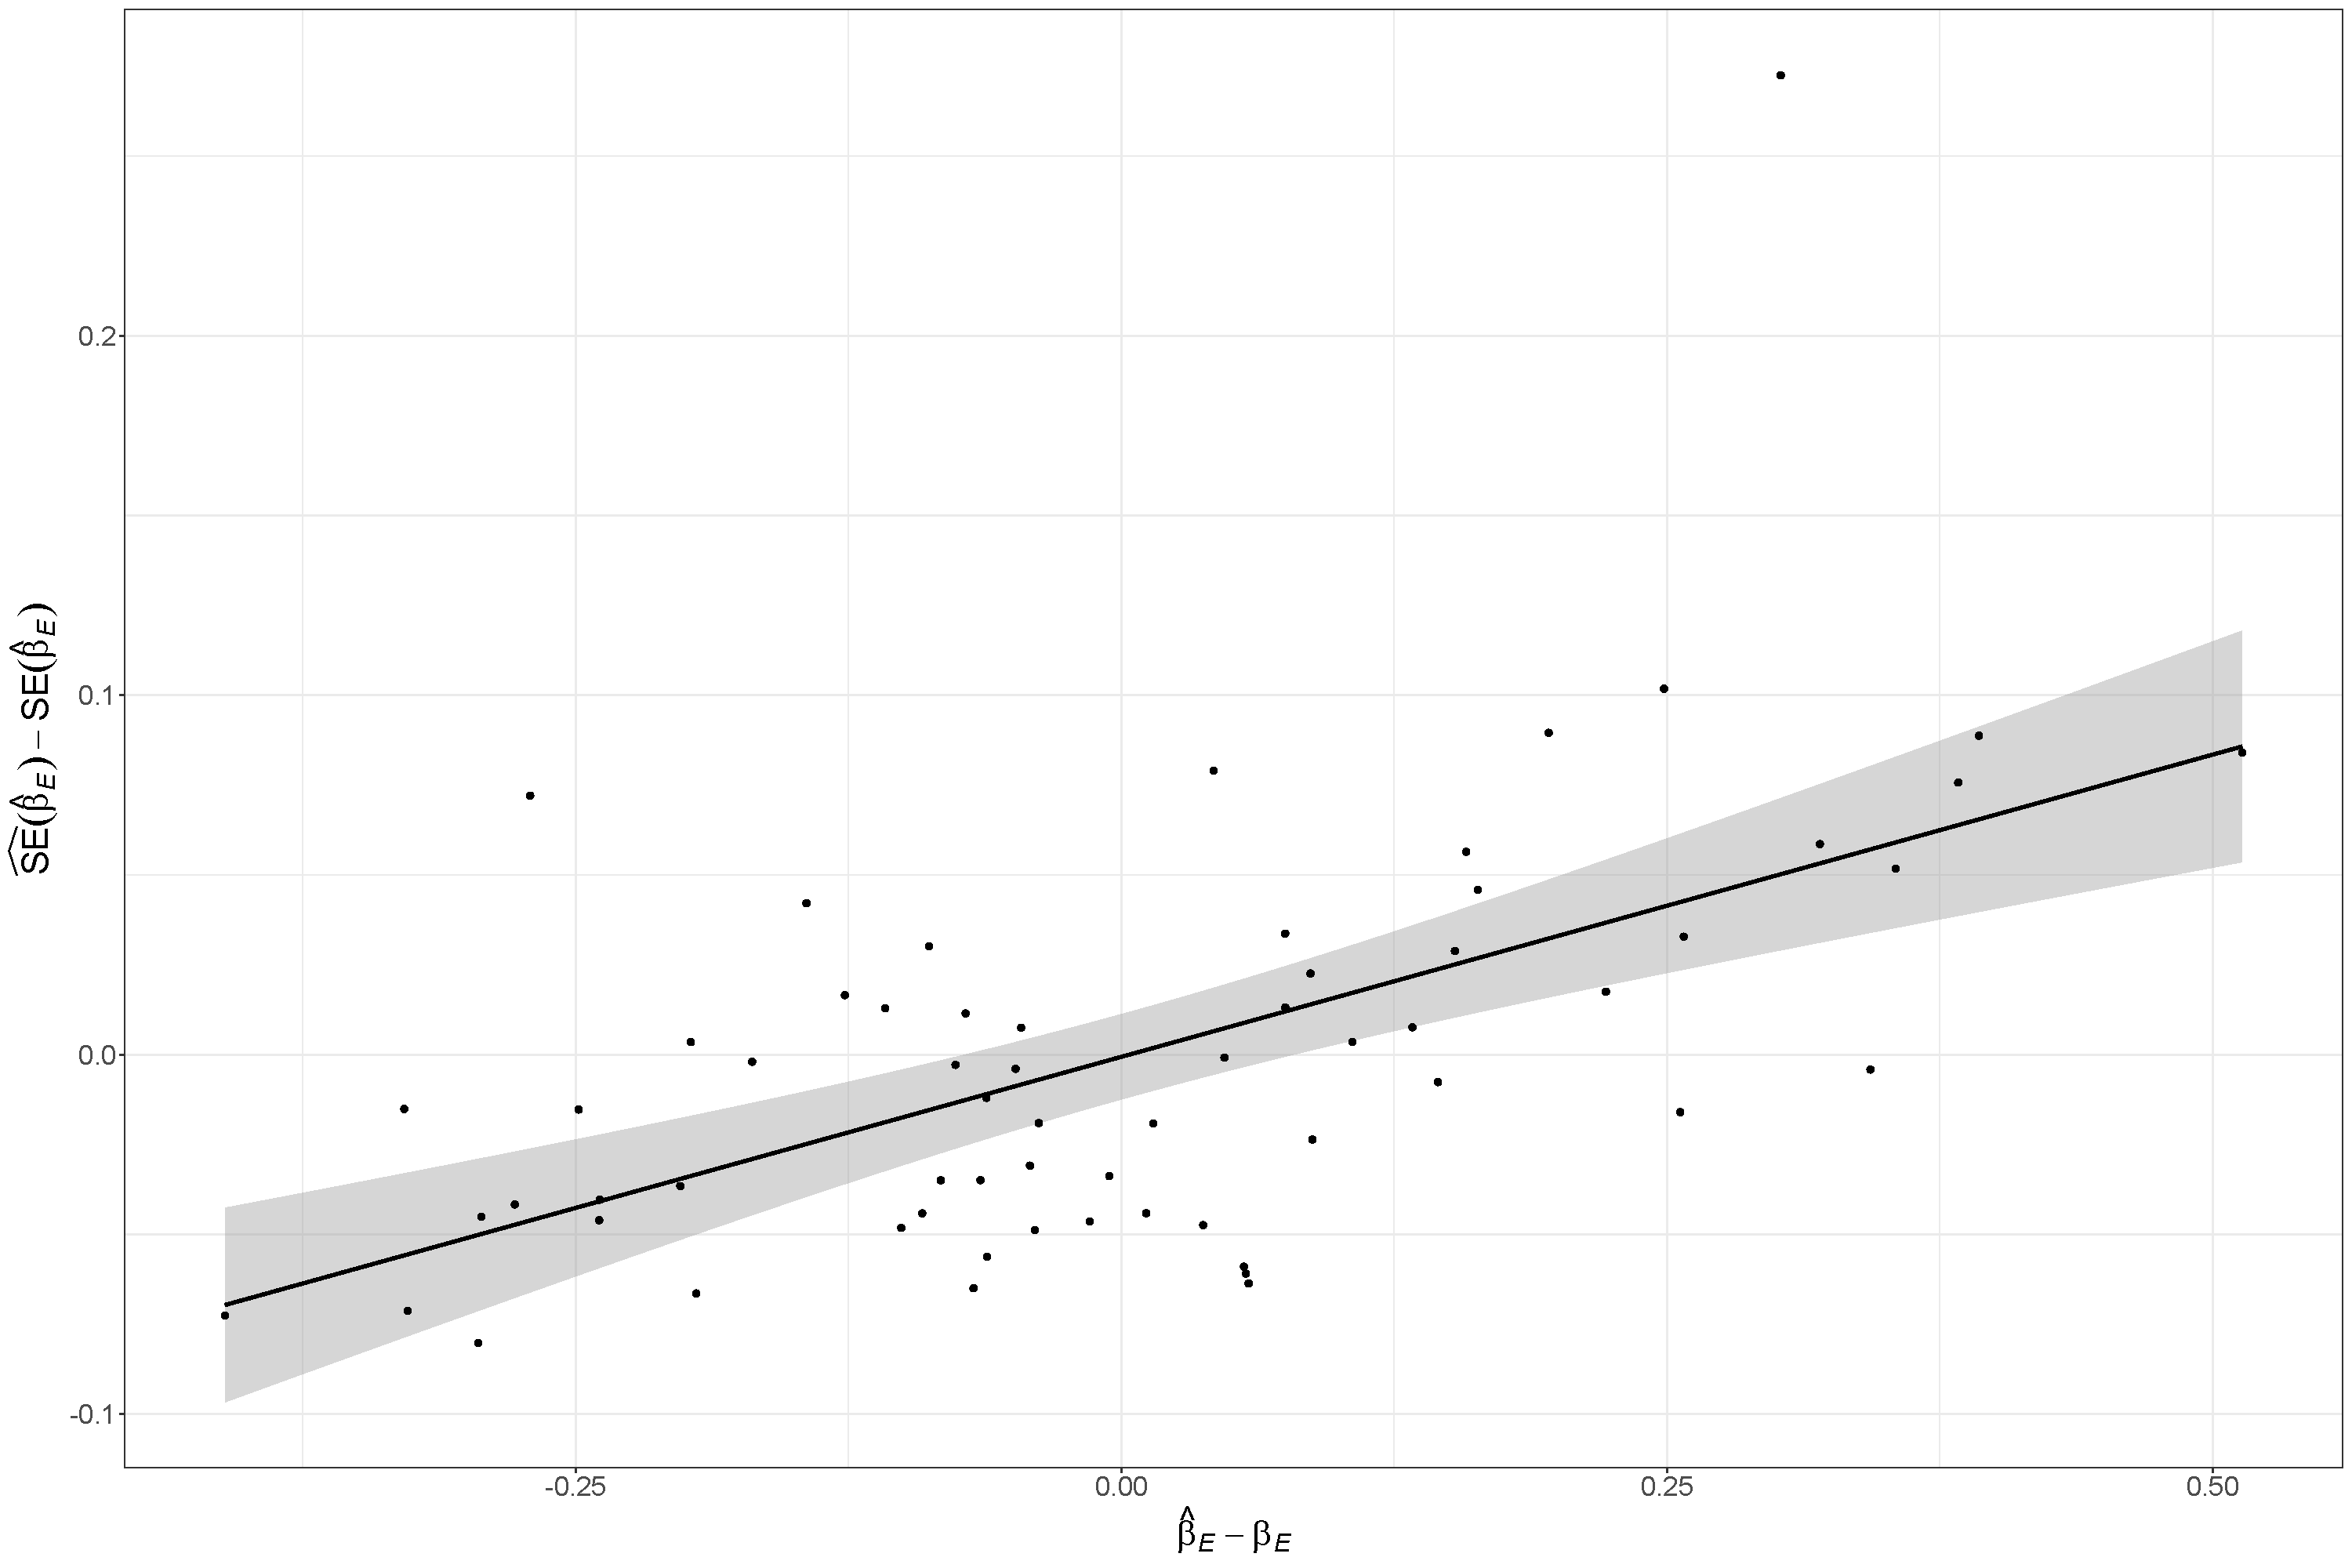
\includegraphics[height = 0.9\textheight]{om_69_em_5_beta_E_se_beta_E_lm_plot}
\end{center}
\caption{Positive correlation of covariate effect estimates and Hessian-based standard error estimates for estimating model that also estimates the median $M$ parameter ($\beta_M$) and has correct R+M process error assumption fitted to simulated data from the operating model with R+M process errors, temporal contrast in fishing pressure, low observation uncertainty for both population ($Low OE$) and covariate observations ($\sigma_e = 0.1$), high and uncorrelated temporal variability in the true covariate ($\sigma_E = 0.5$ and $\rho_E = 0$), and the strongest covariate effect on $M$ ($\beta_E = 0.5$).}\label{ex_lm_beta_E_SE_beta_E}
\end{figure}
\end{landscape}

\begin{landscape}
\begin{figure}
\begin{center}
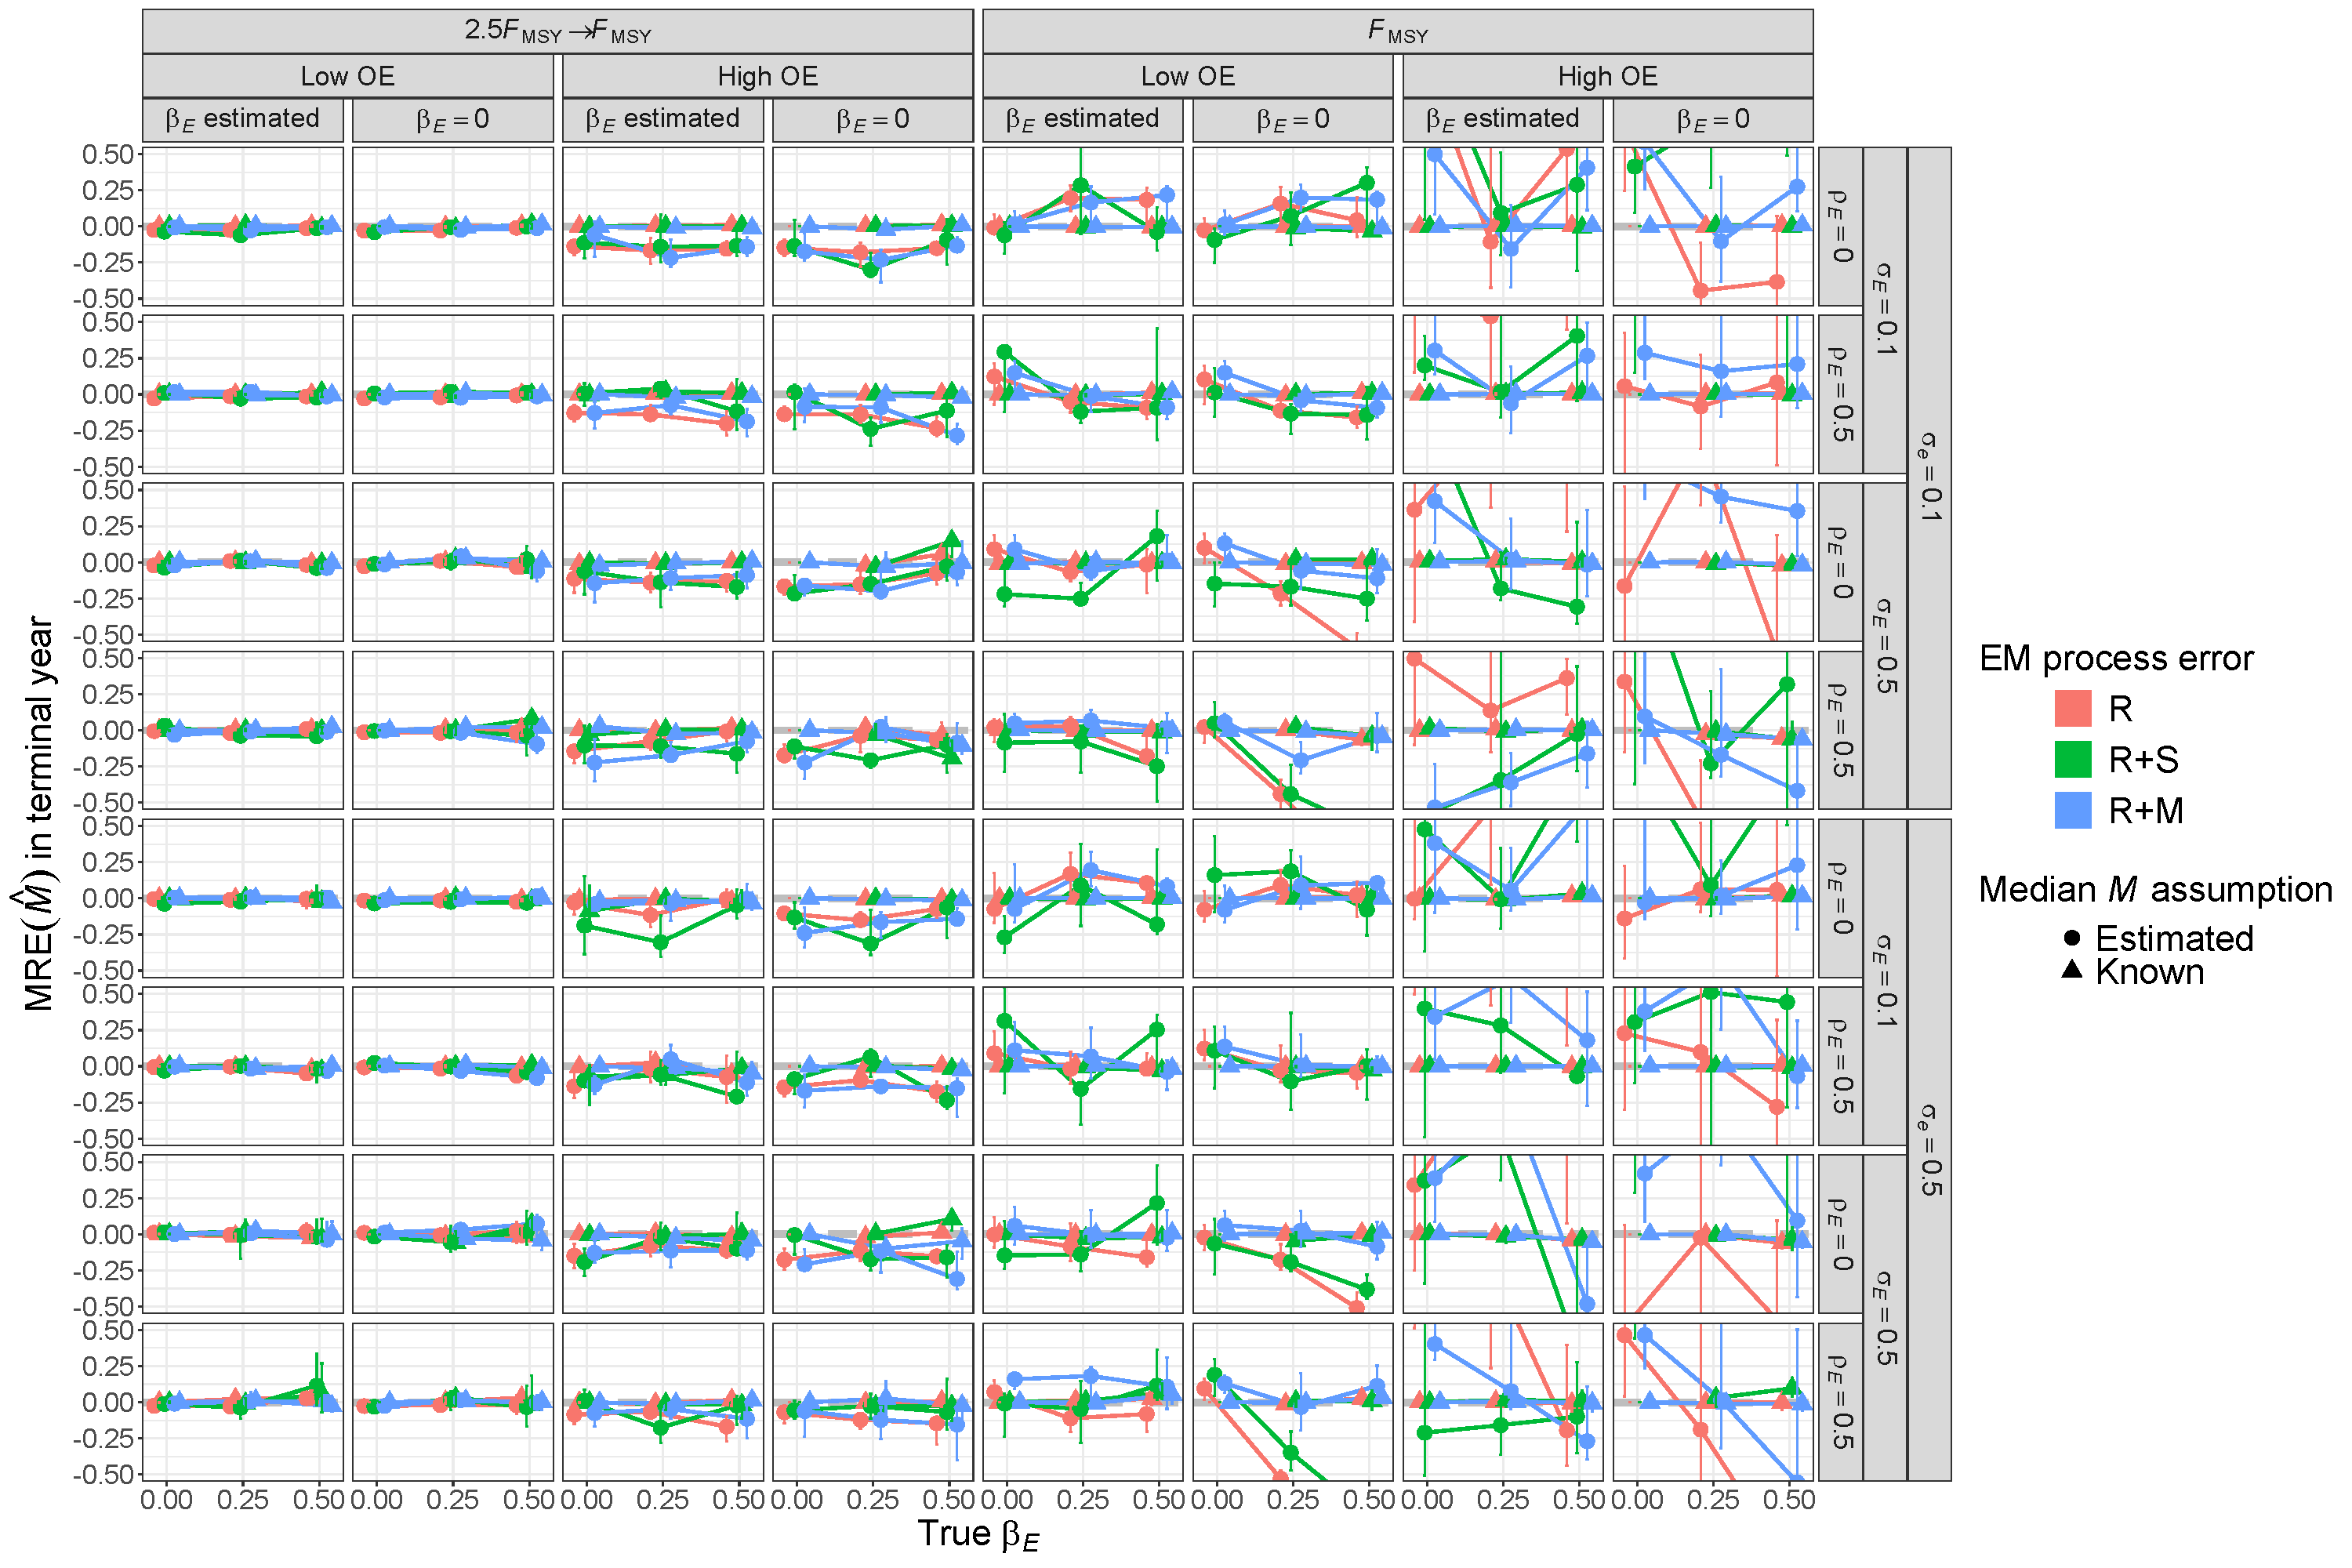
\includegraphics[height = \textheight]{terminal_year_M_bias_Rom}
\end{center}
\caption{For R operating models, median relative error (MRE) of estimates of terminal year $M$ for estimating models with alternative process error assumptions, treatment of covariate effect ($\beta_E = 0$ or estimated), and treatment of median $M$ parameter ($\beta_M$ estimated or known).}\label{terminal_M_bias_Rom}
\end{figure}
\end{landscape}

\begin{landscape}
\begin{figure}
\begin{center}
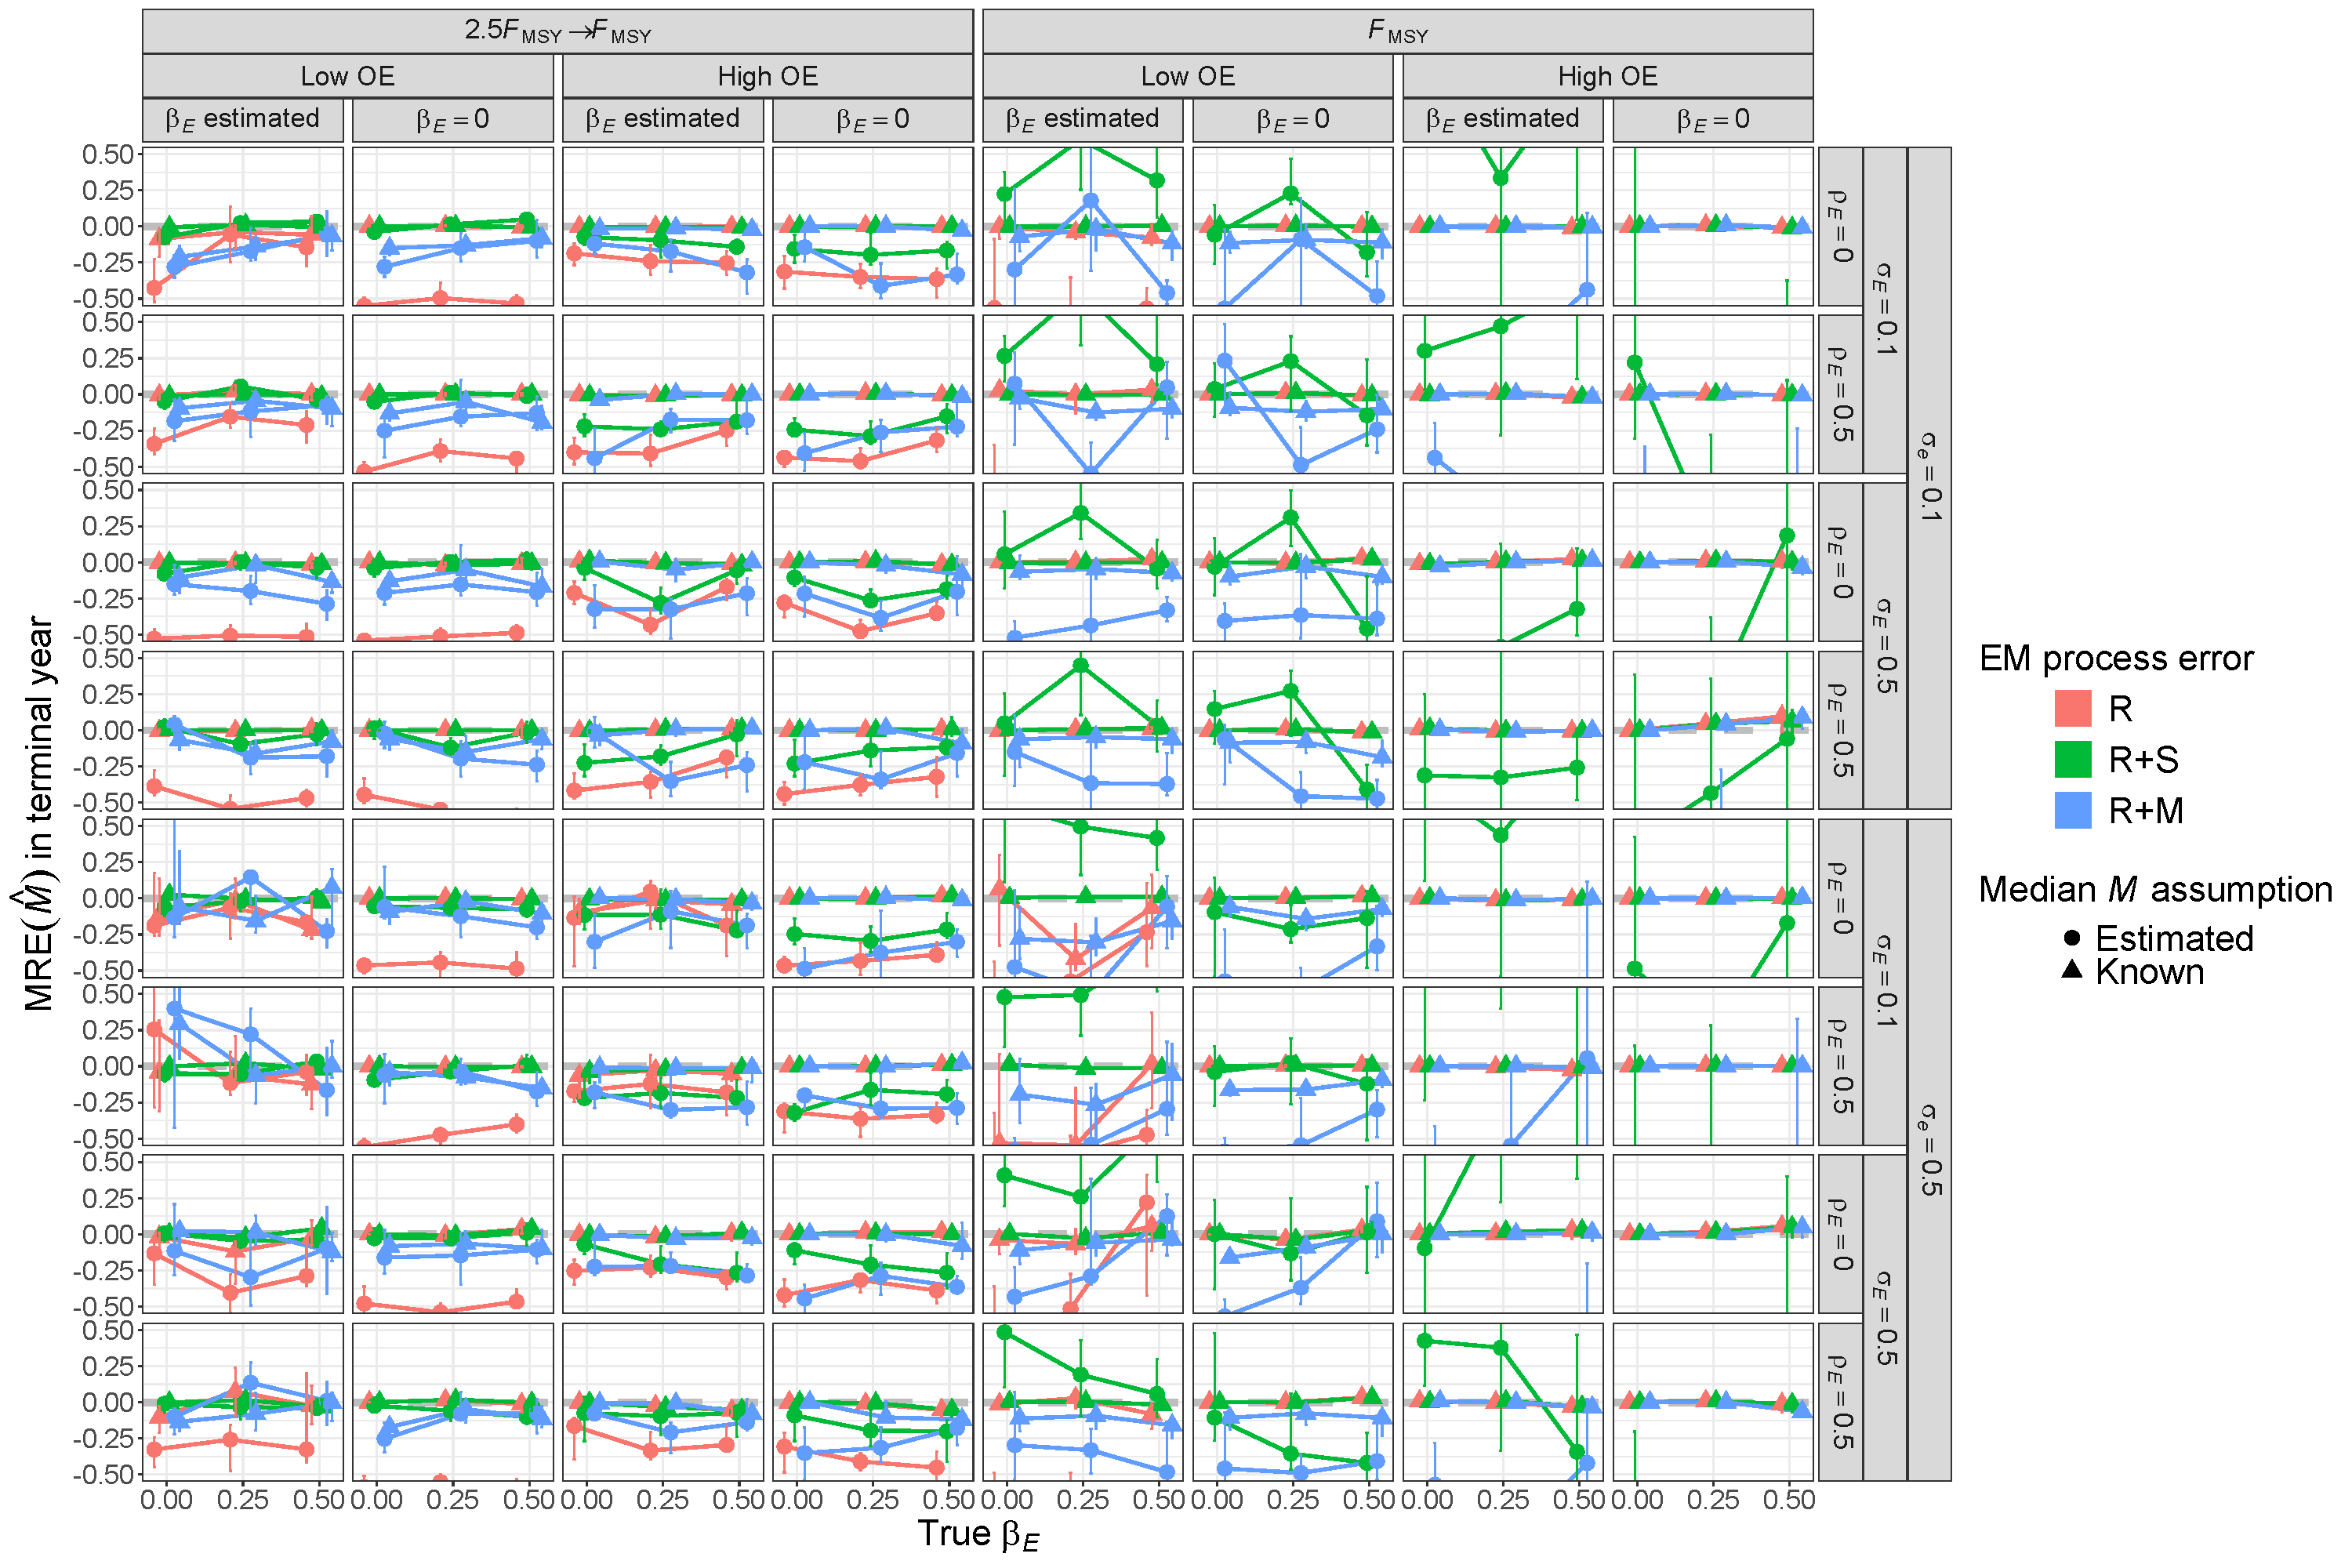
\includegraphics[height = \textheight]{terminal_year_M_bias_RSom}
\end{center}
\caption{For R+S operating models, median relative error (MRE) of estimates of terminal year $M$ for estimating models with alternative process error assumptions, treatment of covariate effect ($\beta_E = 0$ or estimated), and treatment of median $M$ parameter ($\beta_M$ estimated or known).}\label{terminal_M_bias_RSom}
\end{figure}
\end{landscape}

\begin{landscape}
\begin{figure}
\begin{center}
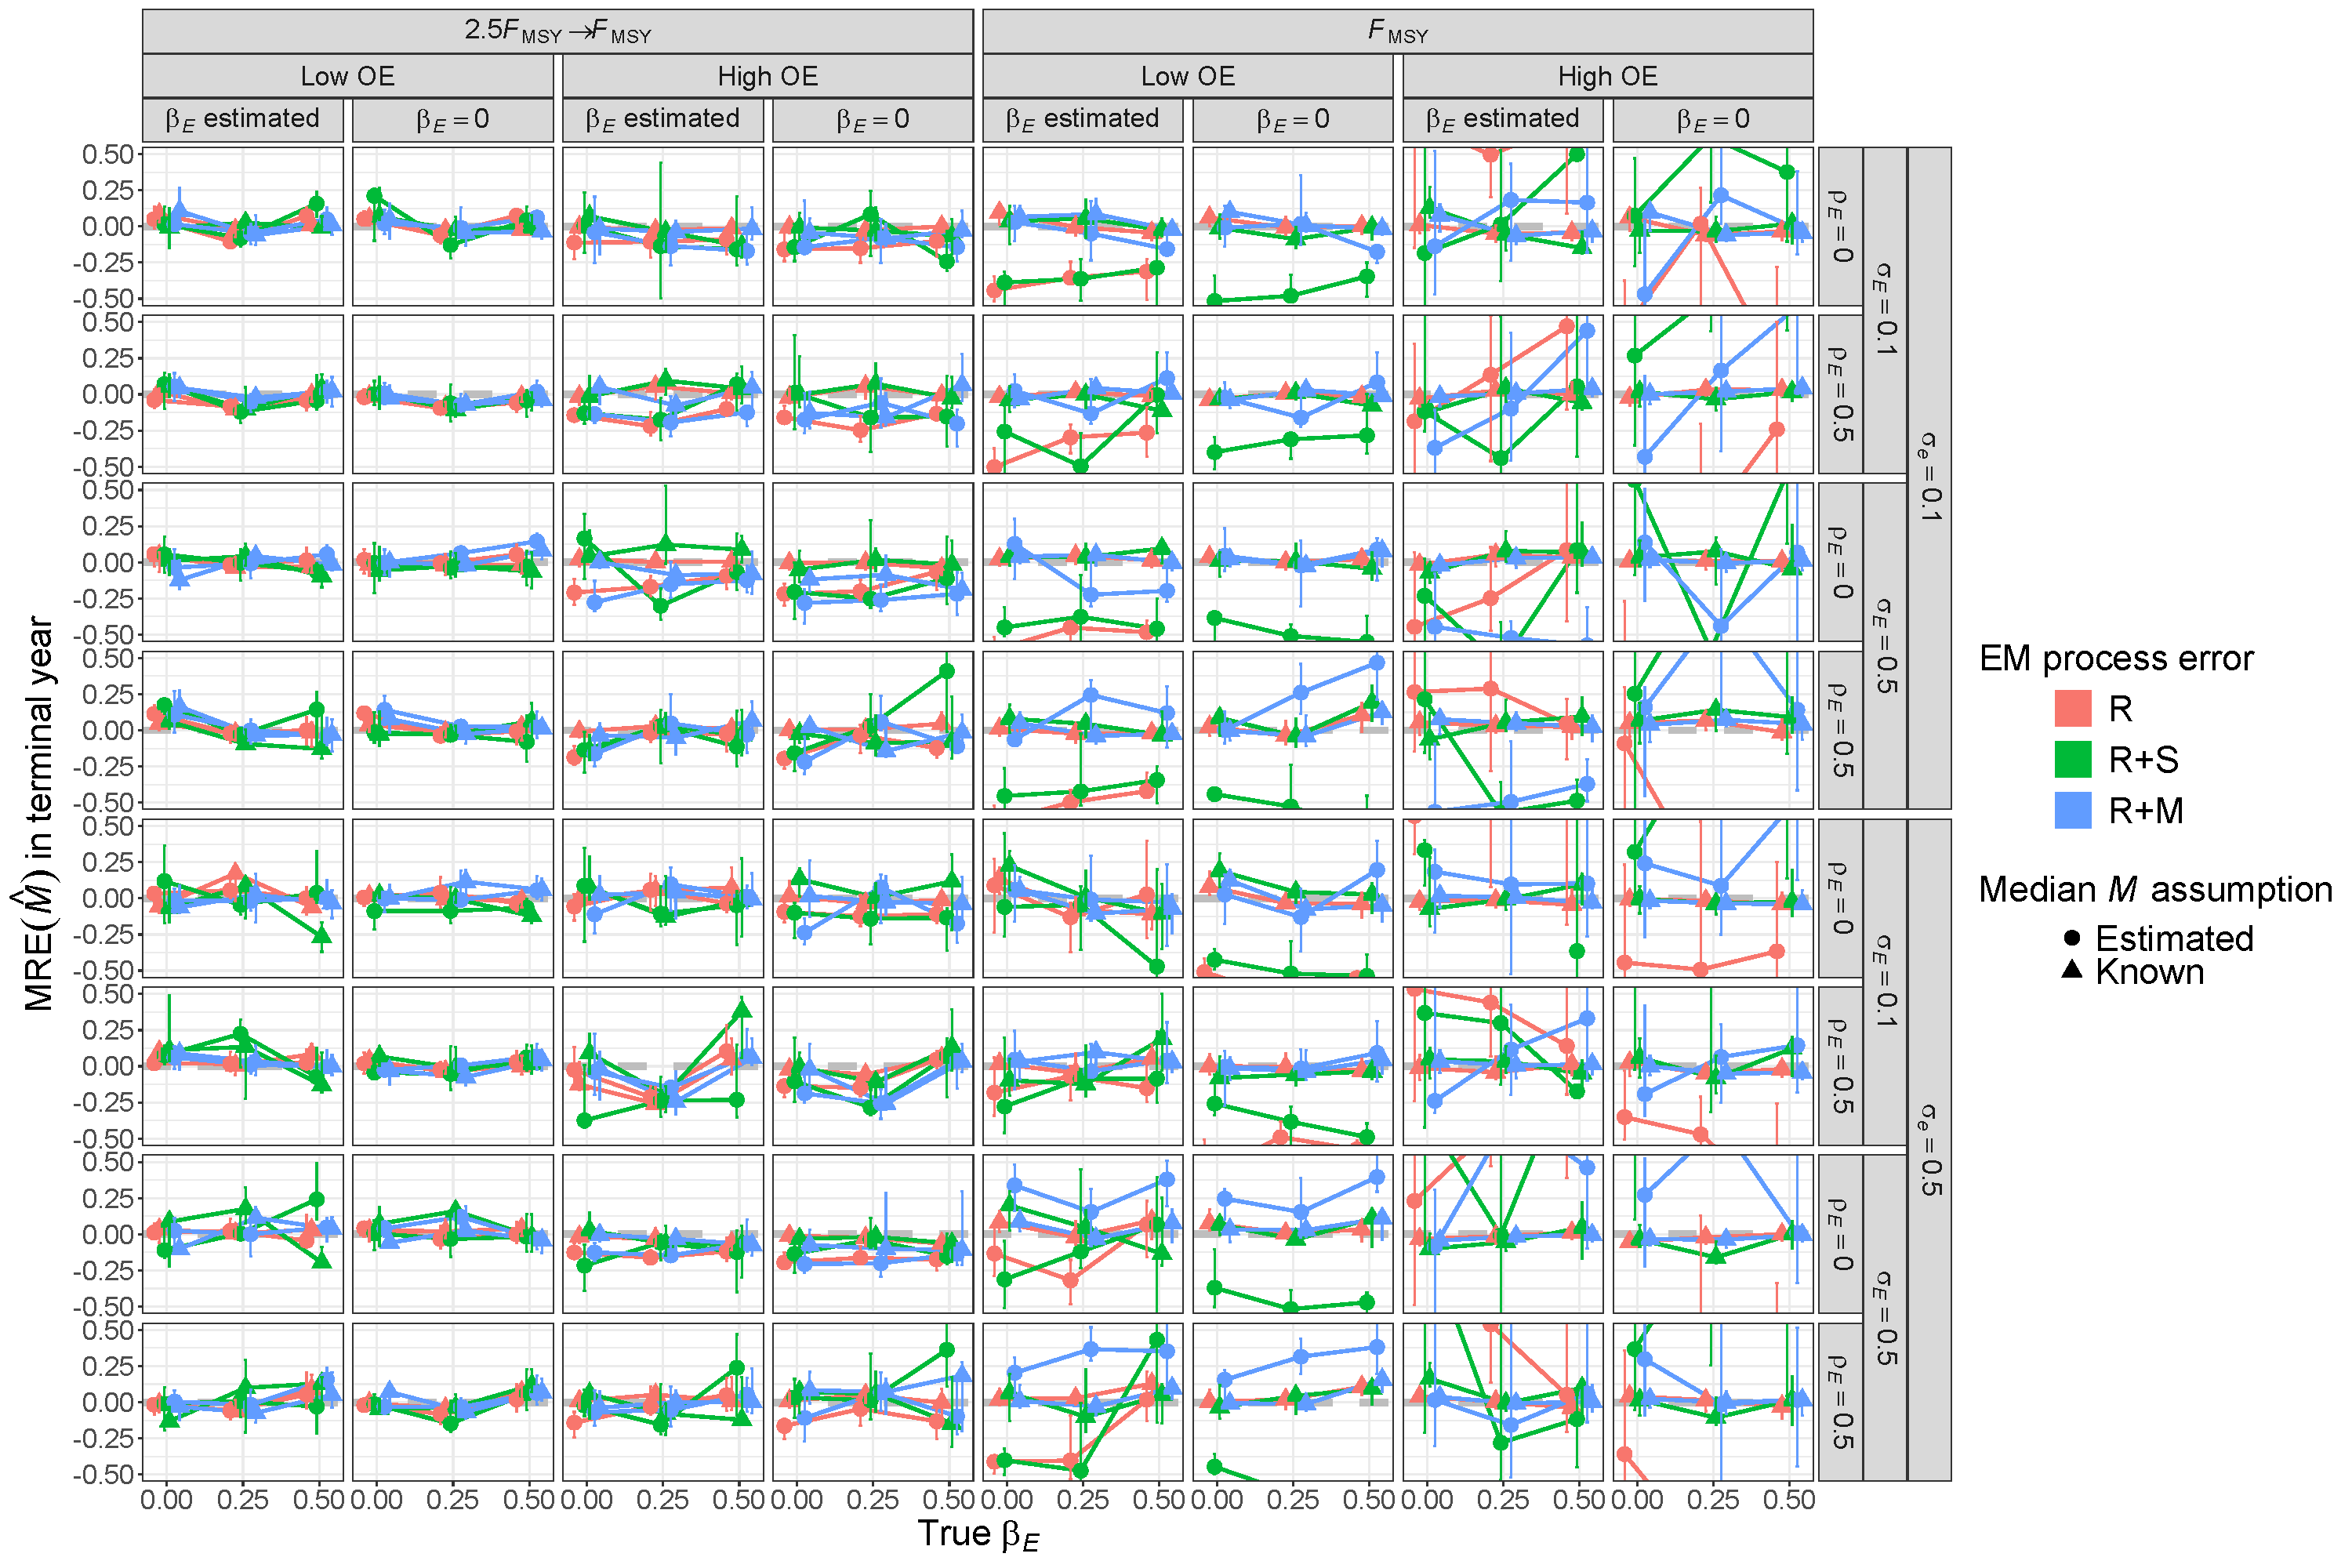
\includegraphics[height = \textheight]{terminal_year_M_bias_RMom}
\end{center}
\caption{For R+M operating models, median relative error (MRE) of estimates of terminal year $M$ for estimating models with alternative process error assumptions, treatment of covariate effect ($\beta_E = 0$ or estimated), and treatment of median $M$ parameter ($\beta_M$ estimated or known).}\label{terminal_M_bias_RMom}
\end{figure}
\end{landscape}

\begin{landscape}
\begin{figure}
\begin{center}
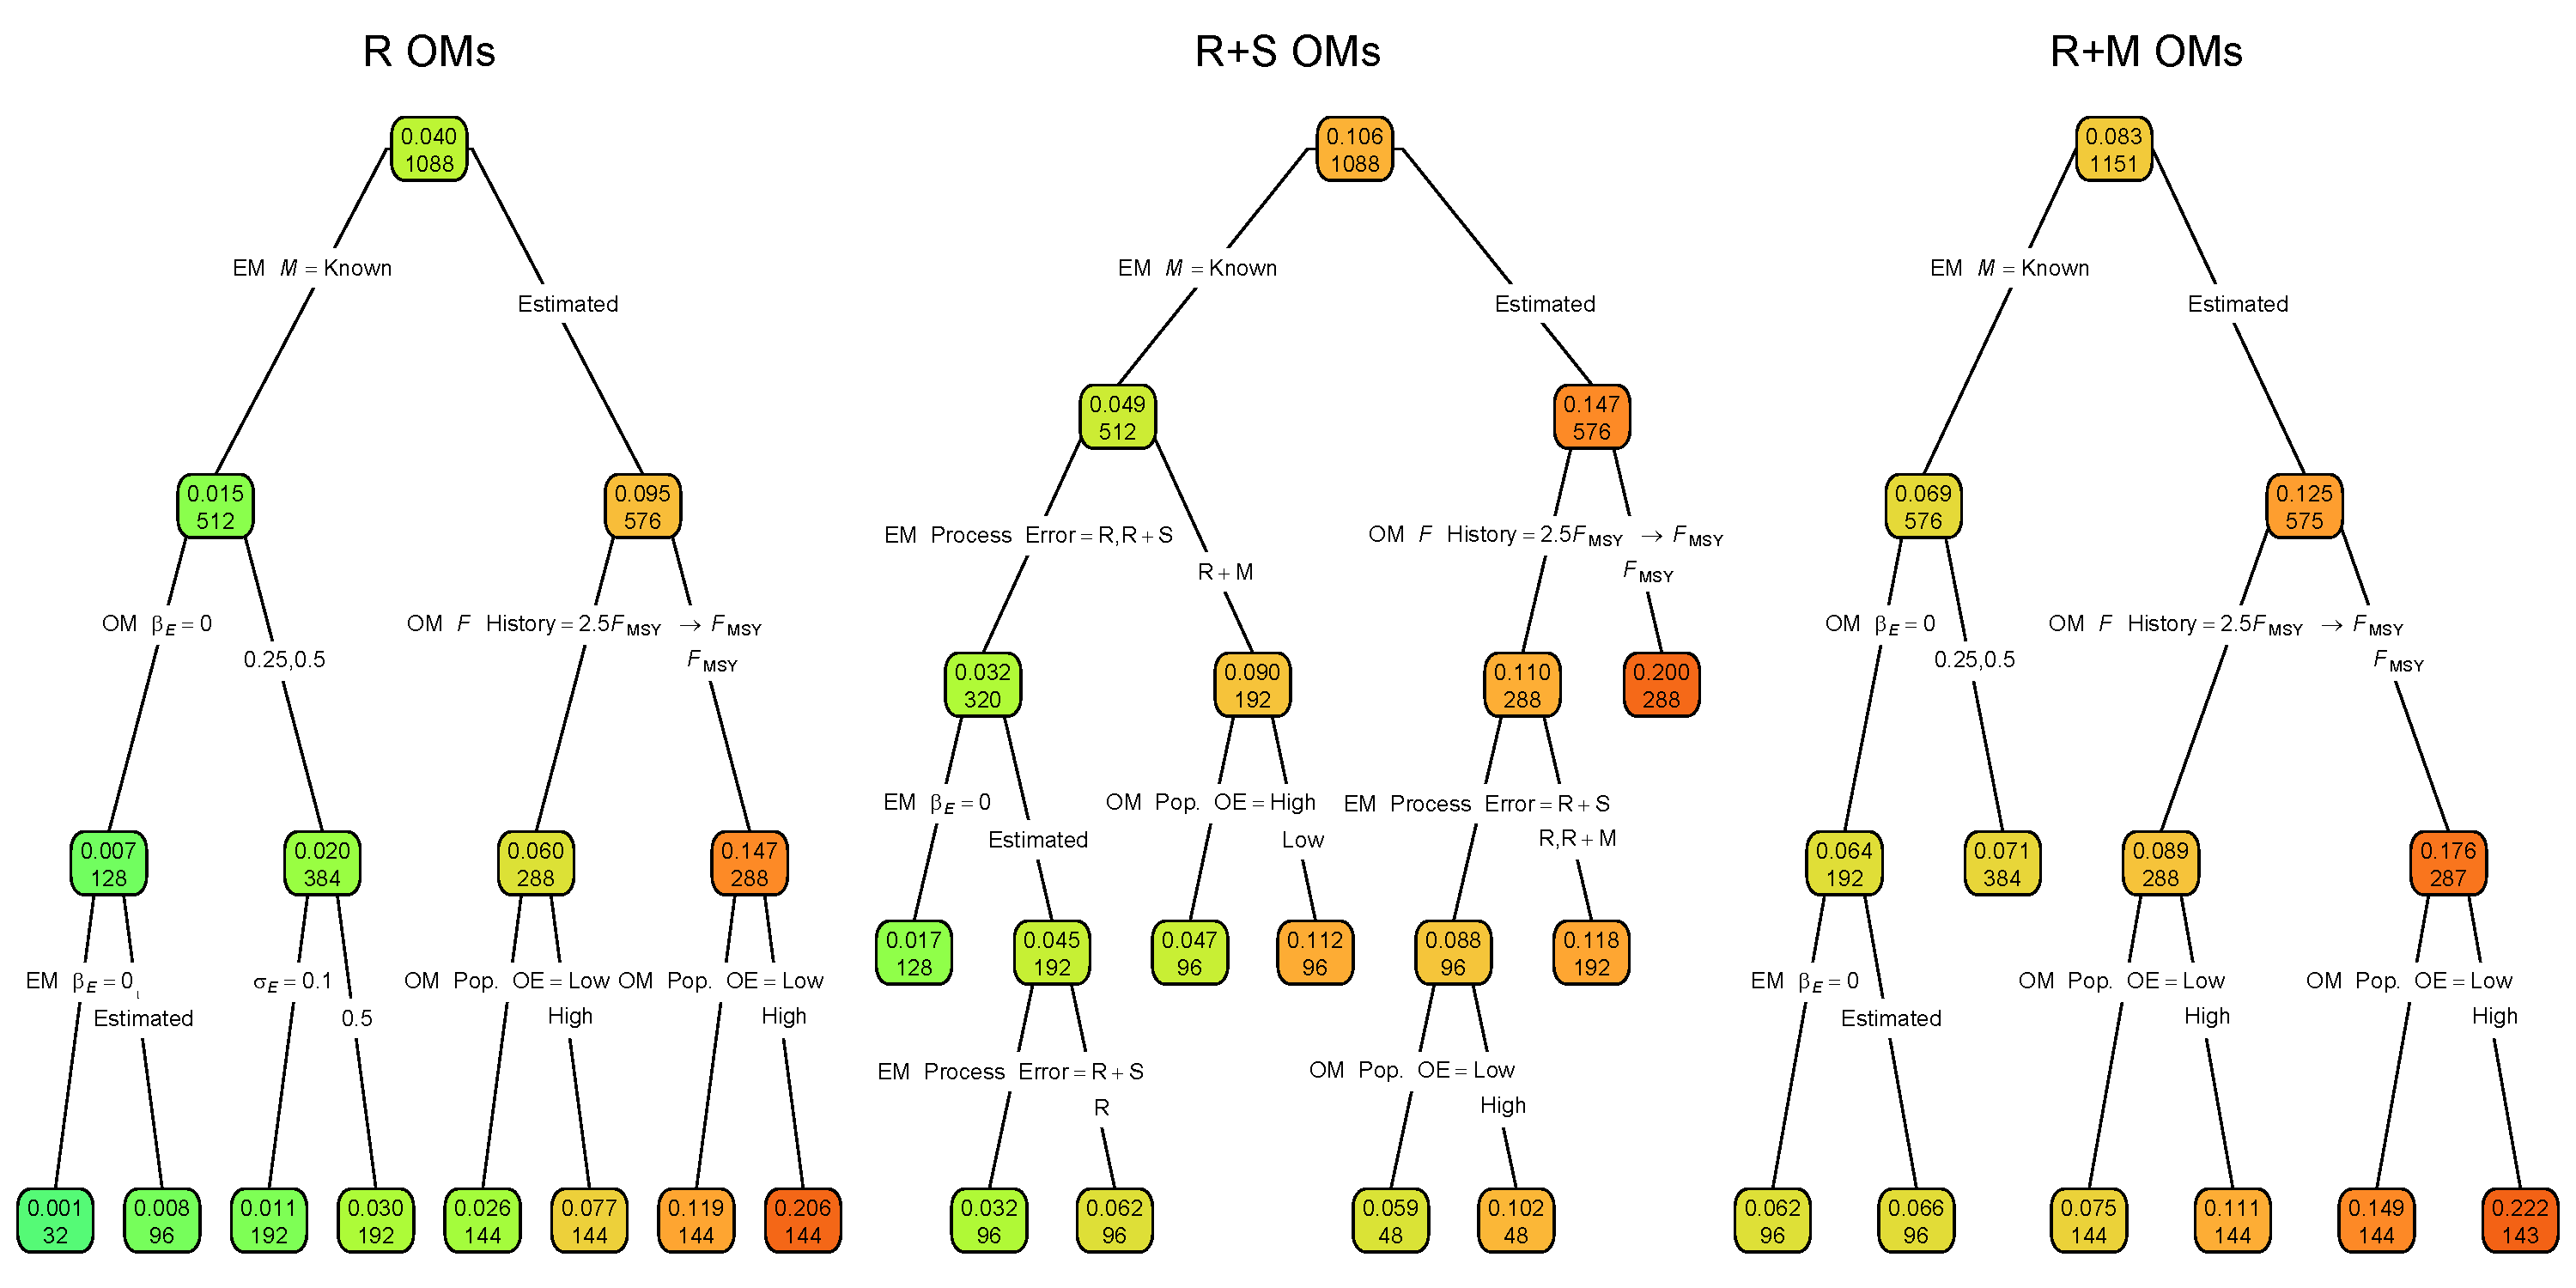
\includegraphics[width = 1.4\textwidth]{term_M_rmse_regtree_plots}
\end{center}
\caption{Regression trees for the log-transformed RMSE of terminal year $M$. Each node shows the median RMSE (top) and number of observations (bottom) for the corresponding subset. Lower or higher median RMSE are indicated by more green or red polygons, respectively. See Figure 1 caption and Table \ref{factor_table} for further details.}\label{term_M_rmse_regtree}
\end{figure}
\end{landscape}

\begin{landscape}
\begin{figure}
\begin{center}
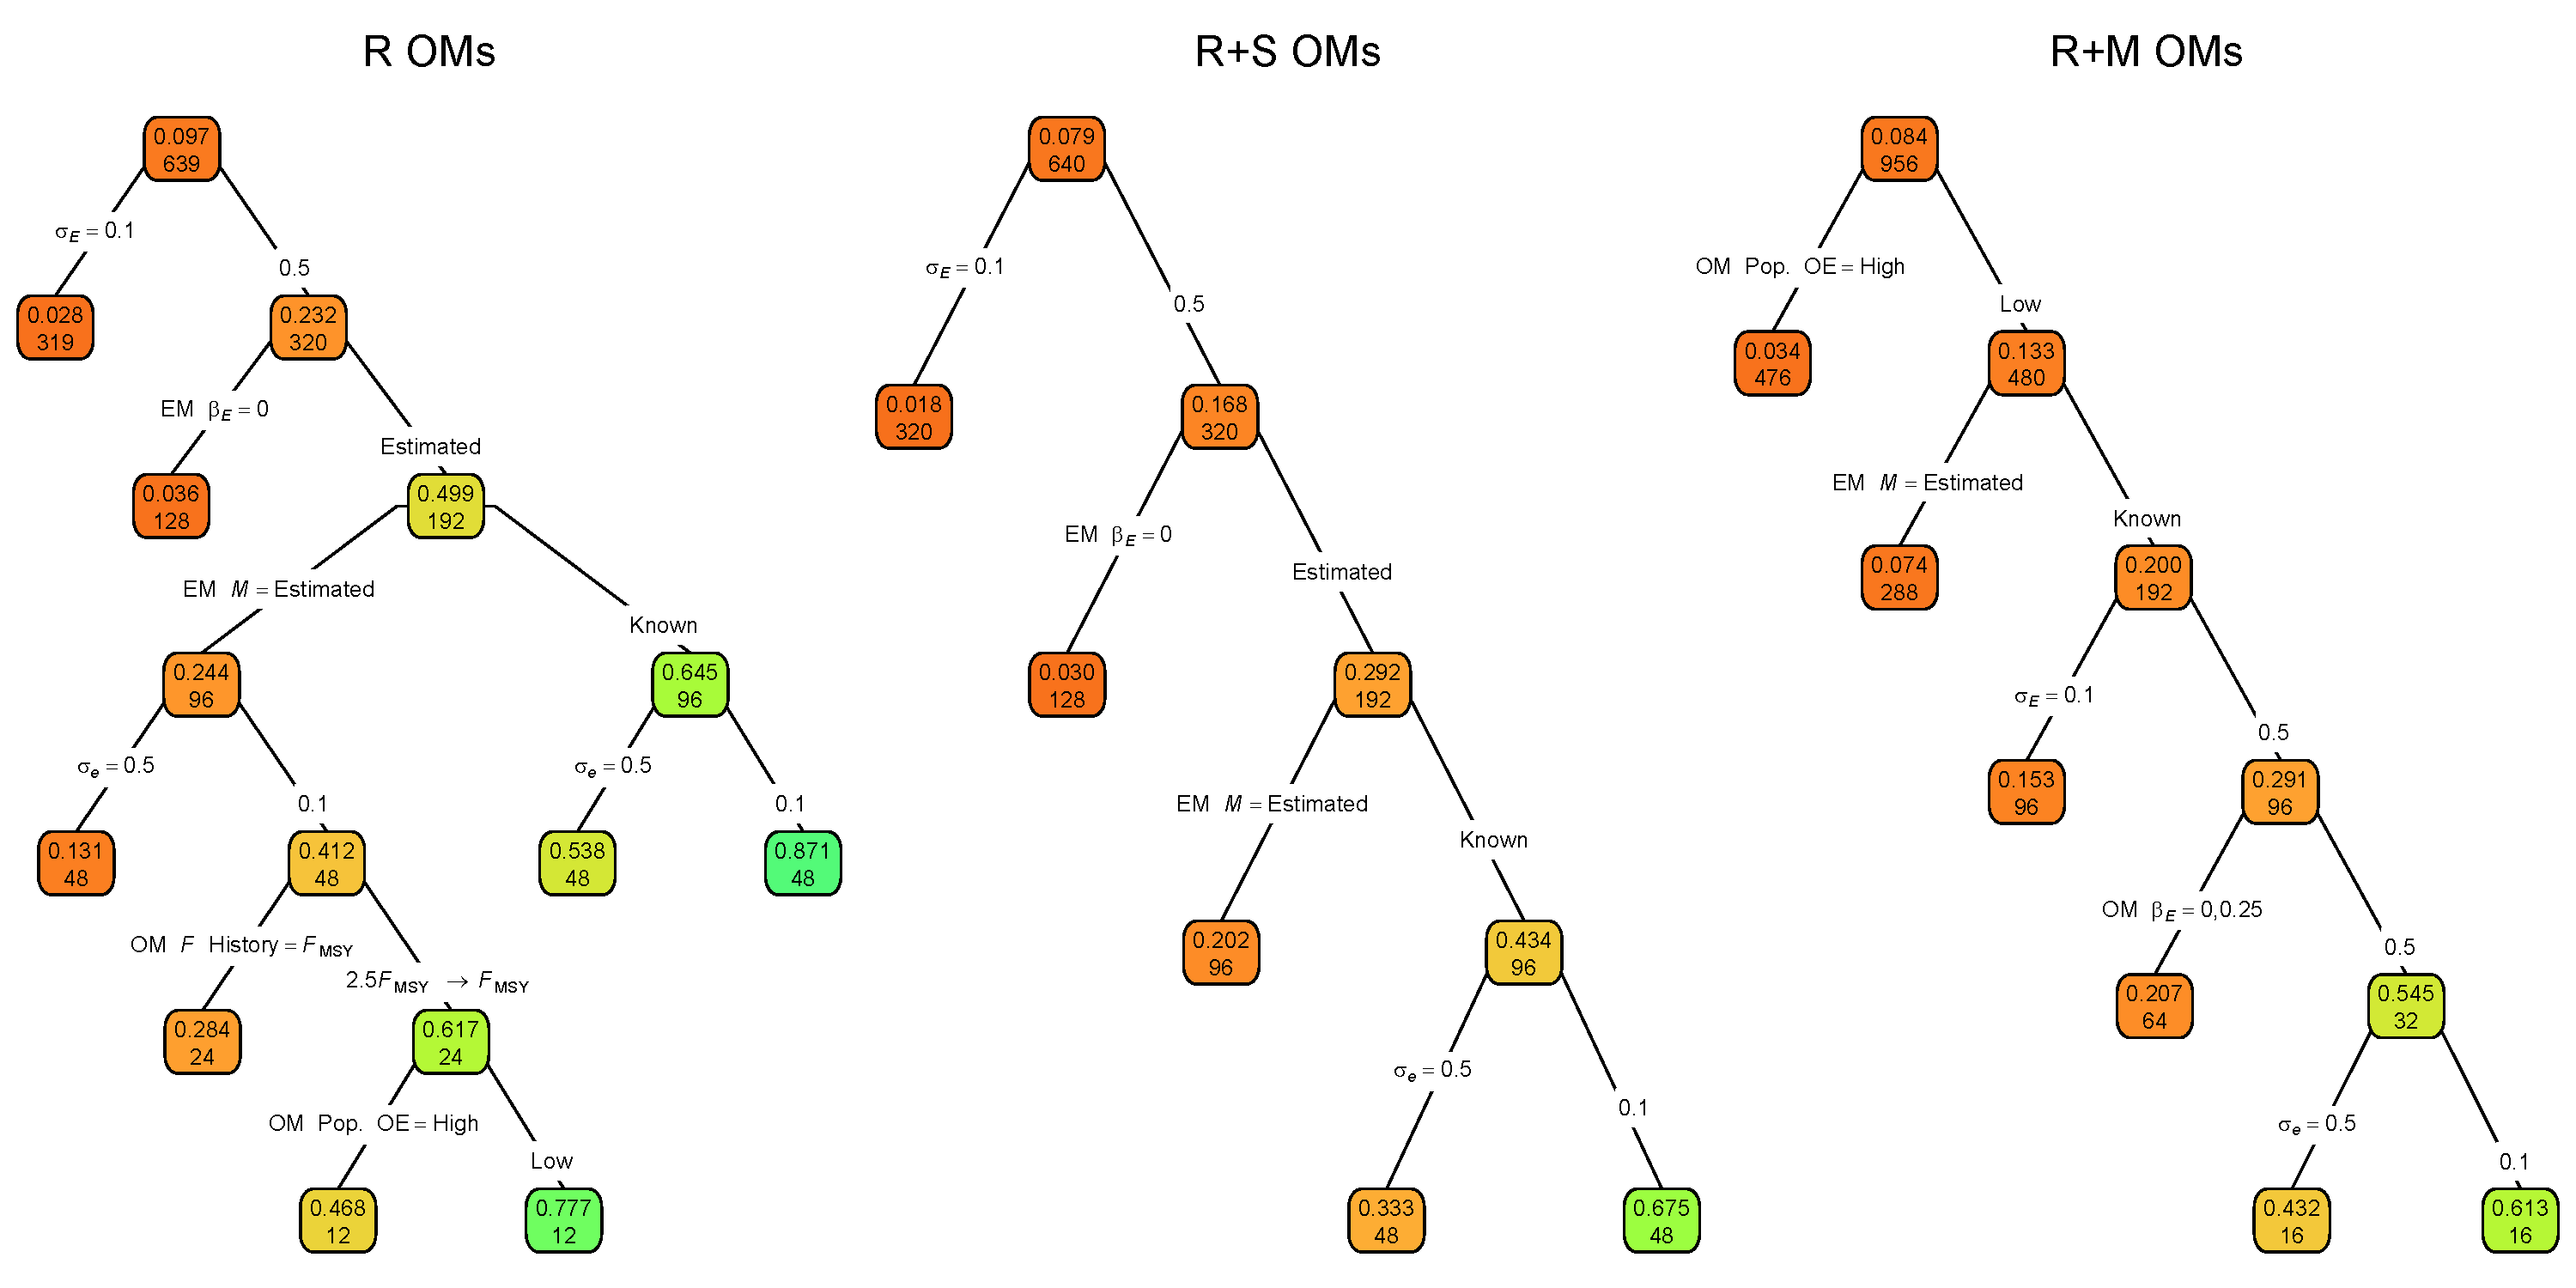
\includegraphics[width = 1.4\textwidth]{term_M_corr_regtree_plots}
\end{center}
\caption{Regression trees for the correlation of terminal year $M$ estimates and true values. Each node shows the median correlation for the corresponding subset. Lower or higher median correlations are indicated by more red or green polygons, respectively. See Figure 1 caption and Table \ref{factor_table} for further details.}\label{term_M_corr_regtree}
\end{figure}
\end{landscape}

\begin{landscape}
\begin{figure}
\begin{center}
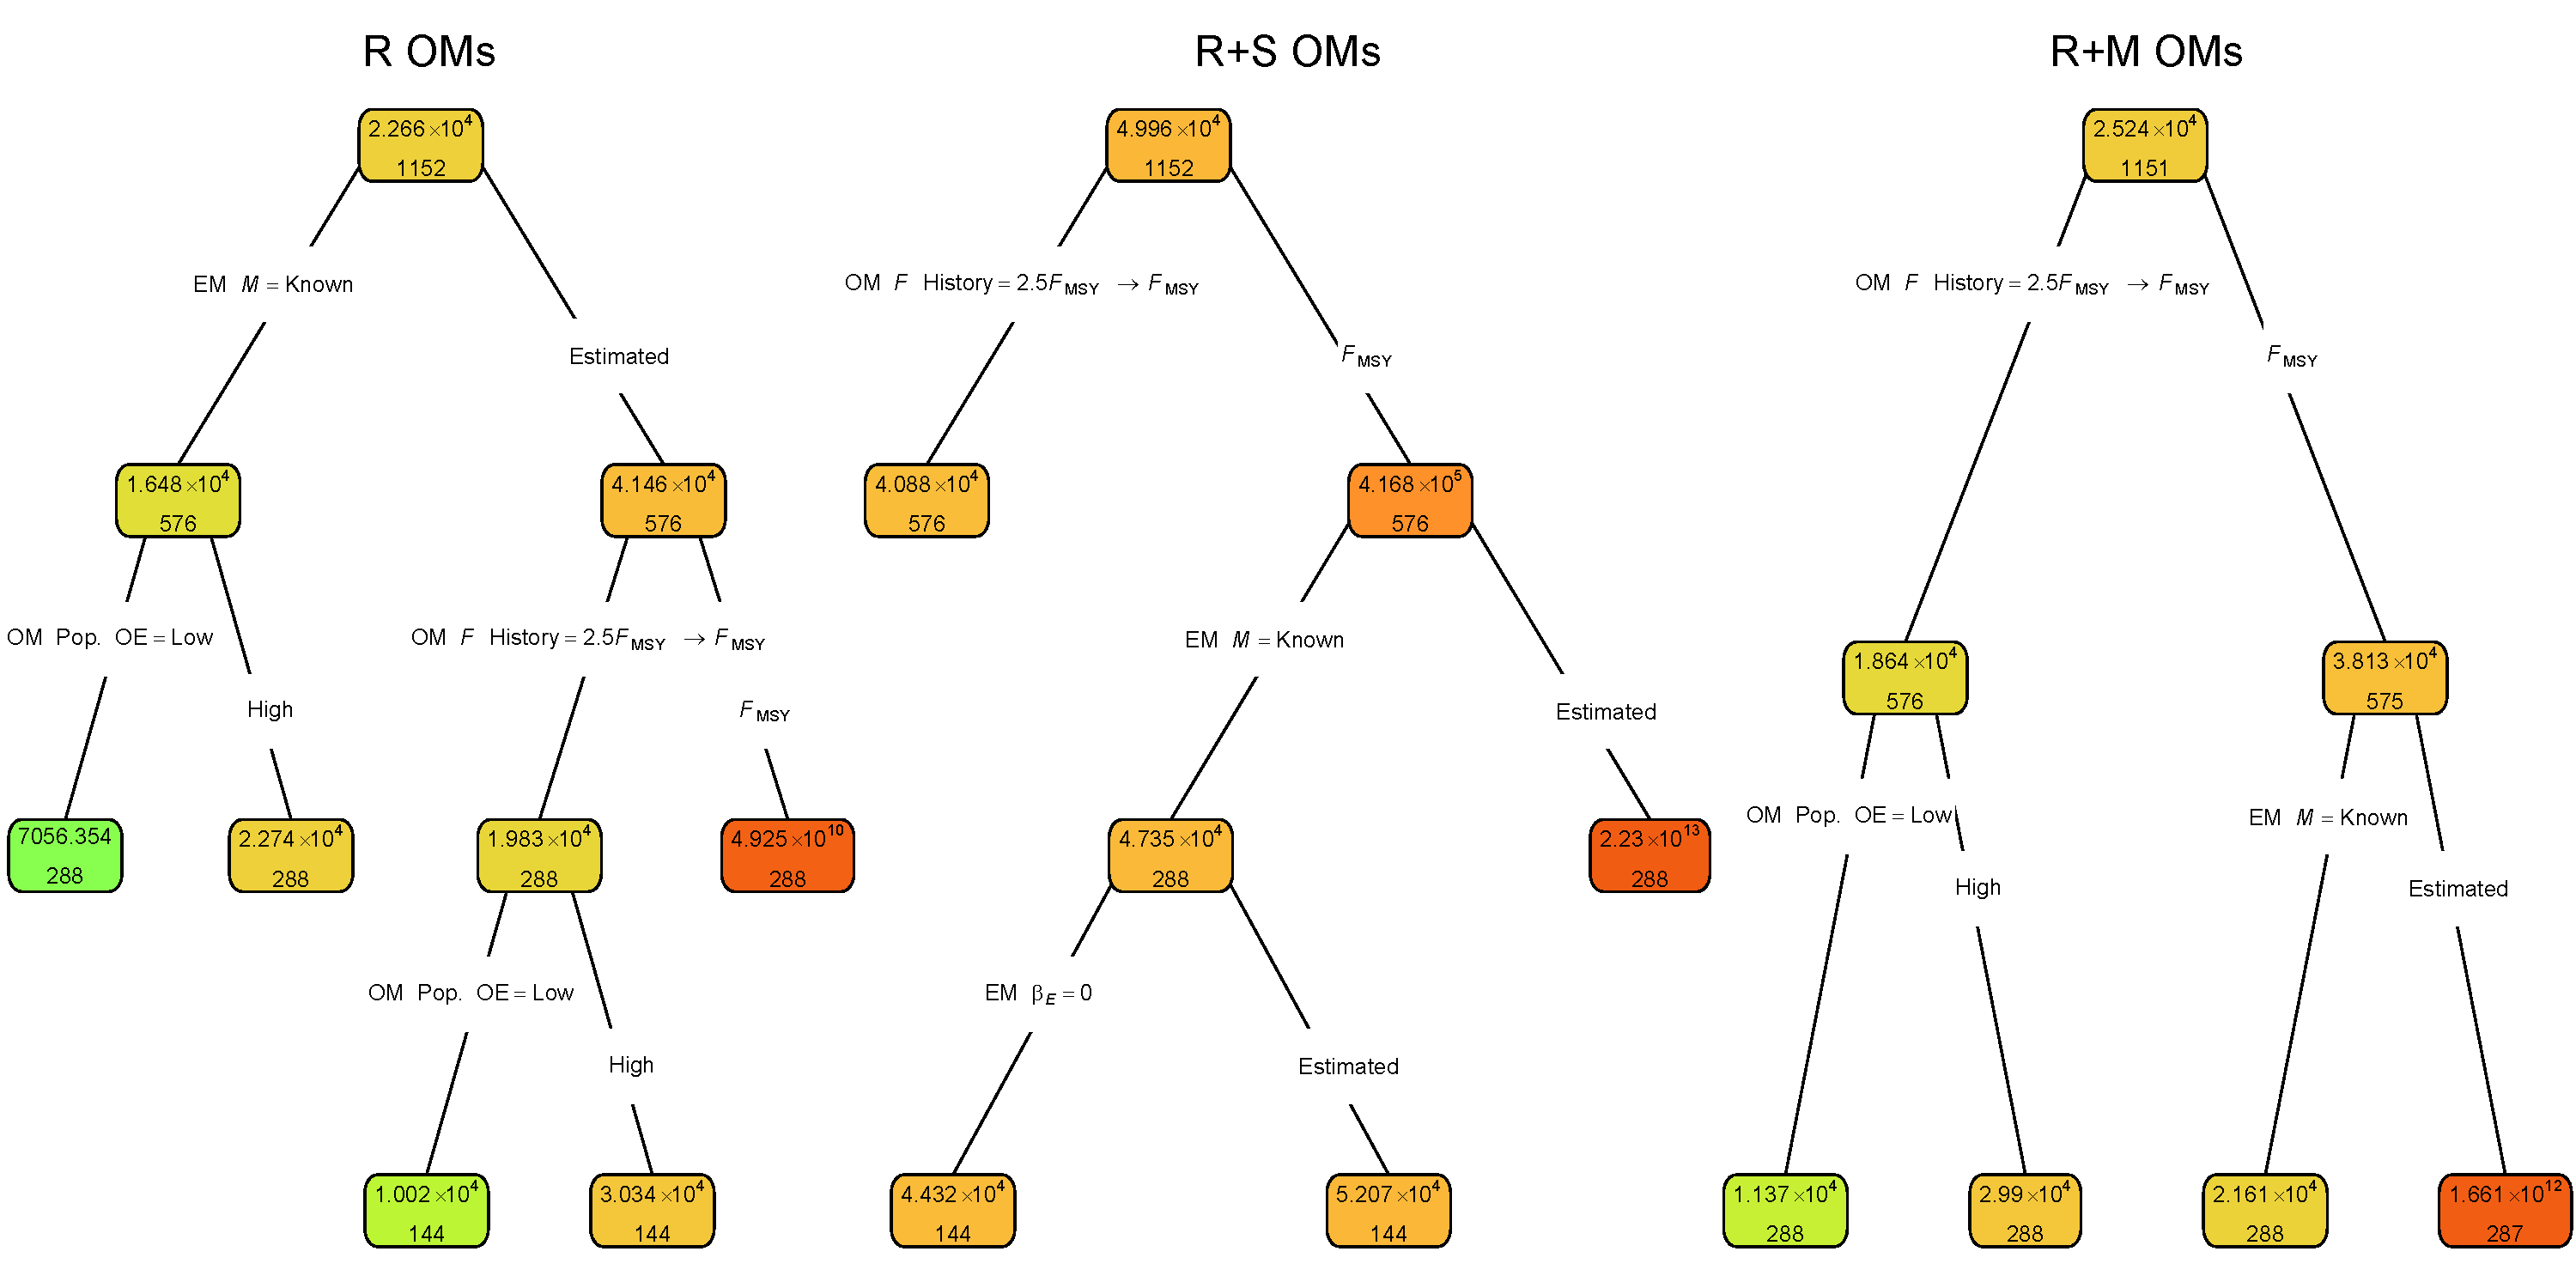
\includegraphics[width = 1.4\textwidth]{term_SSB_rmse_regtree_plots}
\end{center}
\caption{Regression trees for the log-transformed RMSE of terminal year SSB. Each node shows the median RMSE (top) and number of observations (bottom) for the corresponding subset. Lower or higher median RMSE are indicated by more red or green polygons, respectively.}\label{term_SSB_rmse_regtree}
\end{figure}
\end{landscape}

\begin{landscape}
\begin{figure}
\begin{center}
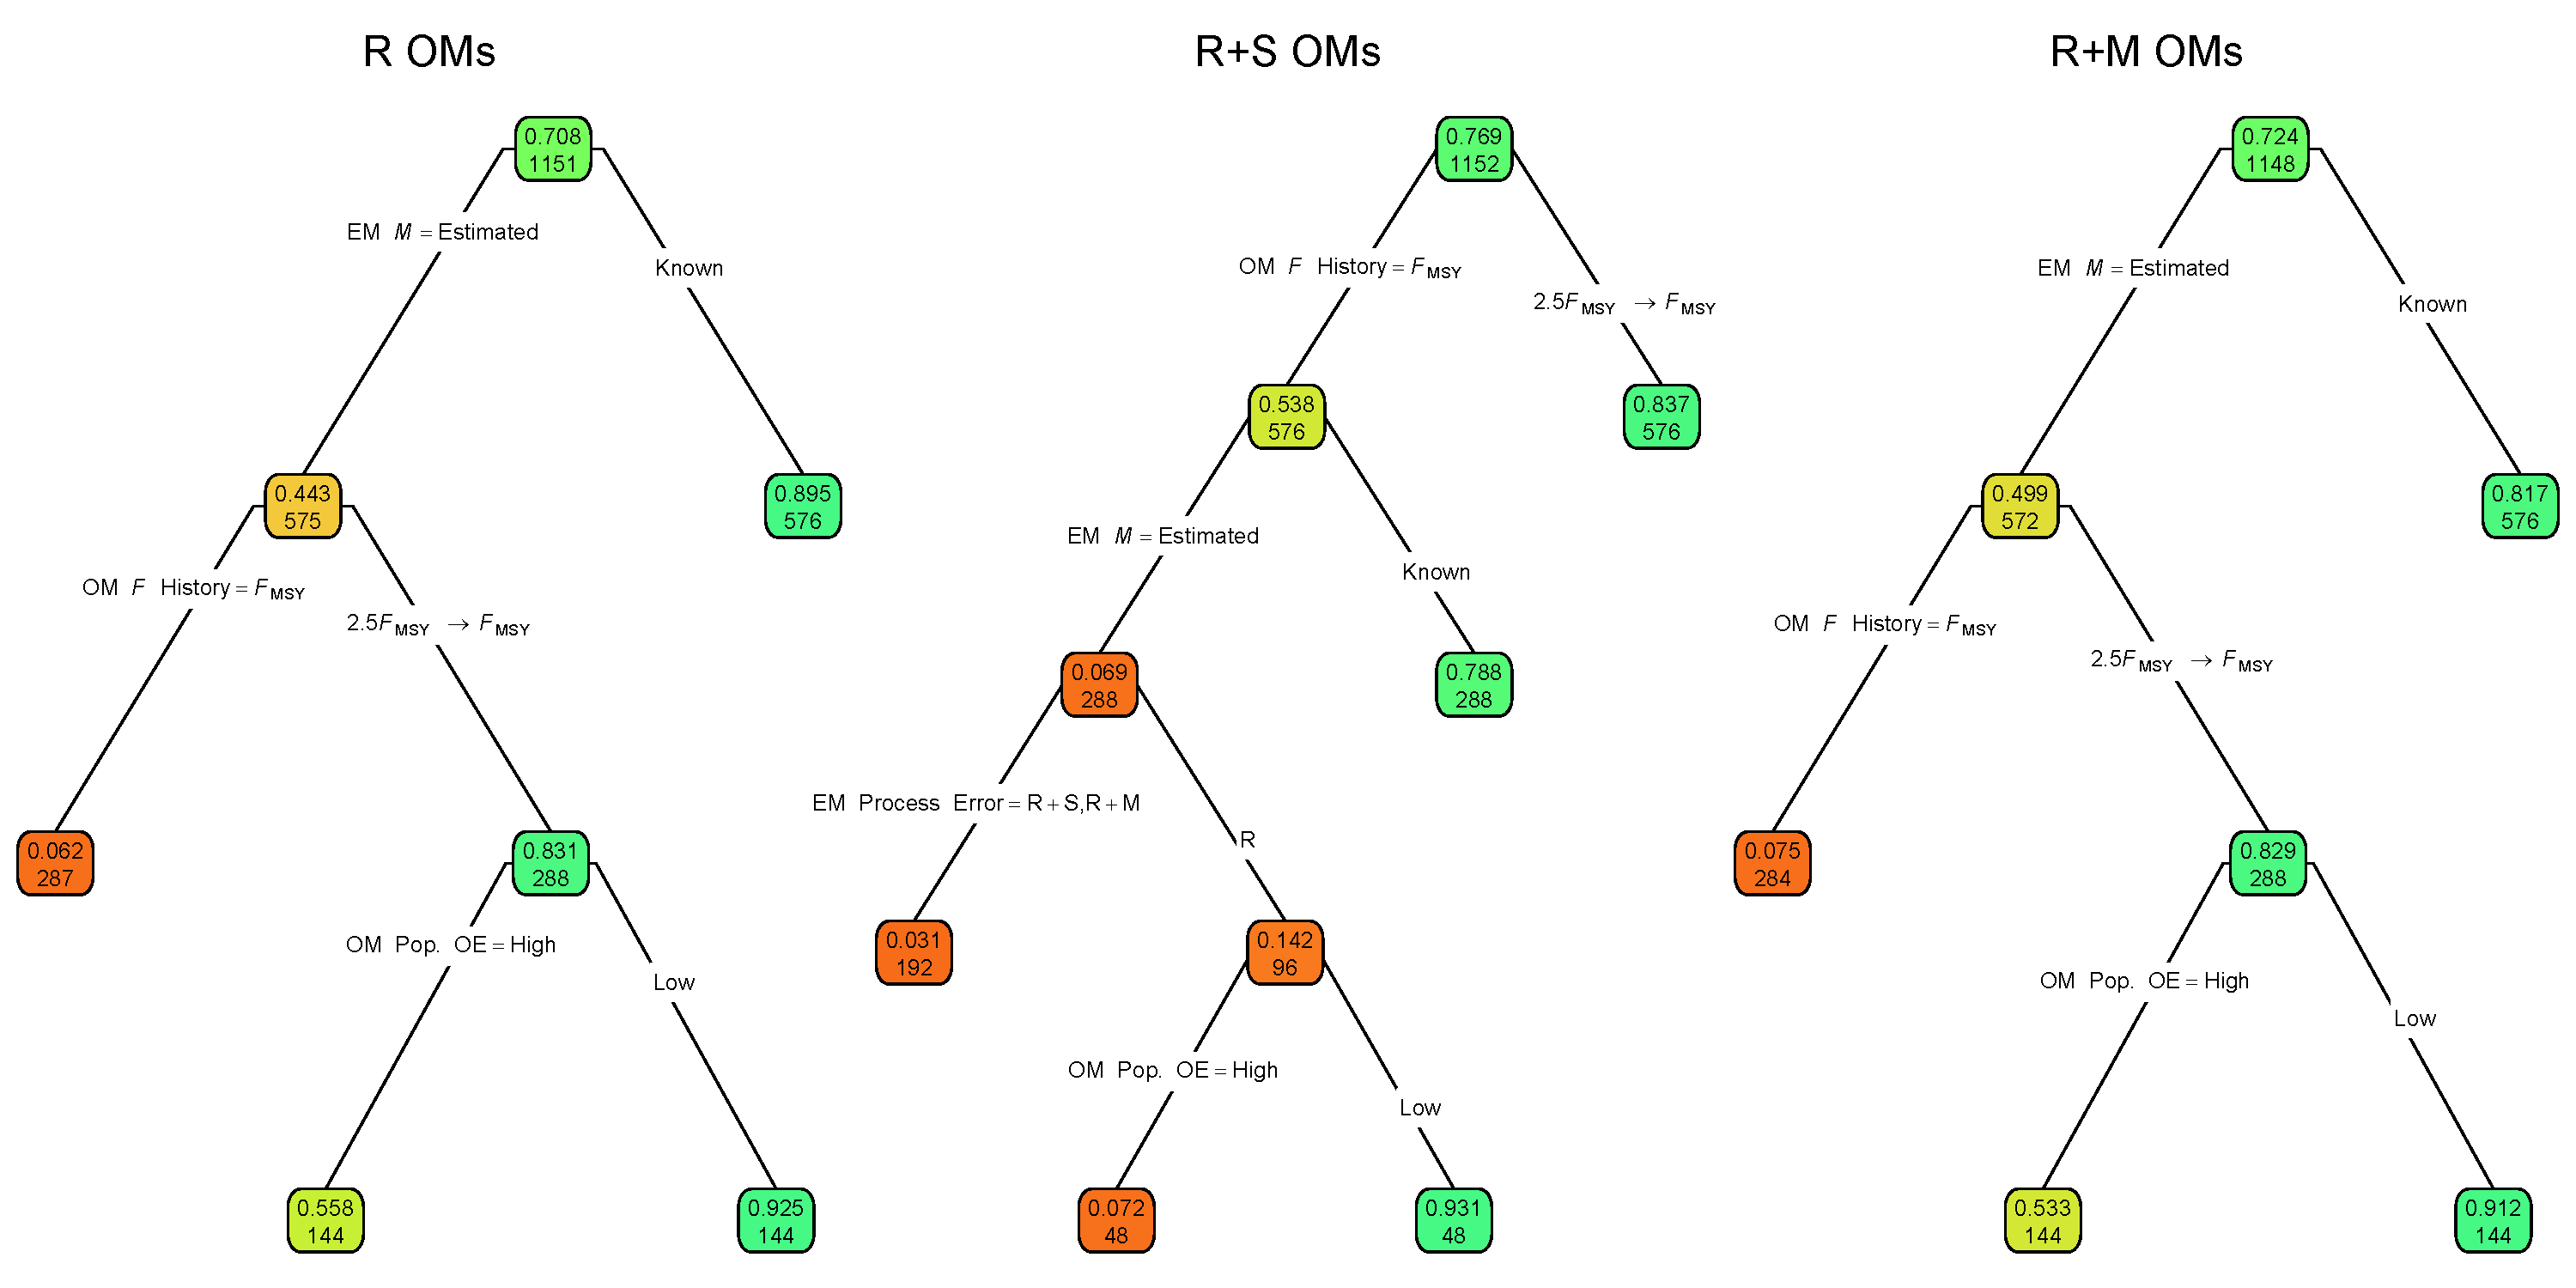
\includegraphics[width = 1.4\textwidth]{term_ssb_corr_regtree_plots}
\end{center}
\caption{Regression trees for the correlation of terminal year SSB estimates and true values. Each node shows the median correlation for the corresponding subset. Lower or higher median correlations are indicated by more red or green polygons, respectively. See Figure 1 caption and Table \ref{factor_table} for further details.}\label{term_ssb_corr_regtree}
\end{figure}
\end{landscape}
\pagebreak

\begin{landscape}
\begin{figure}
\begin{center}
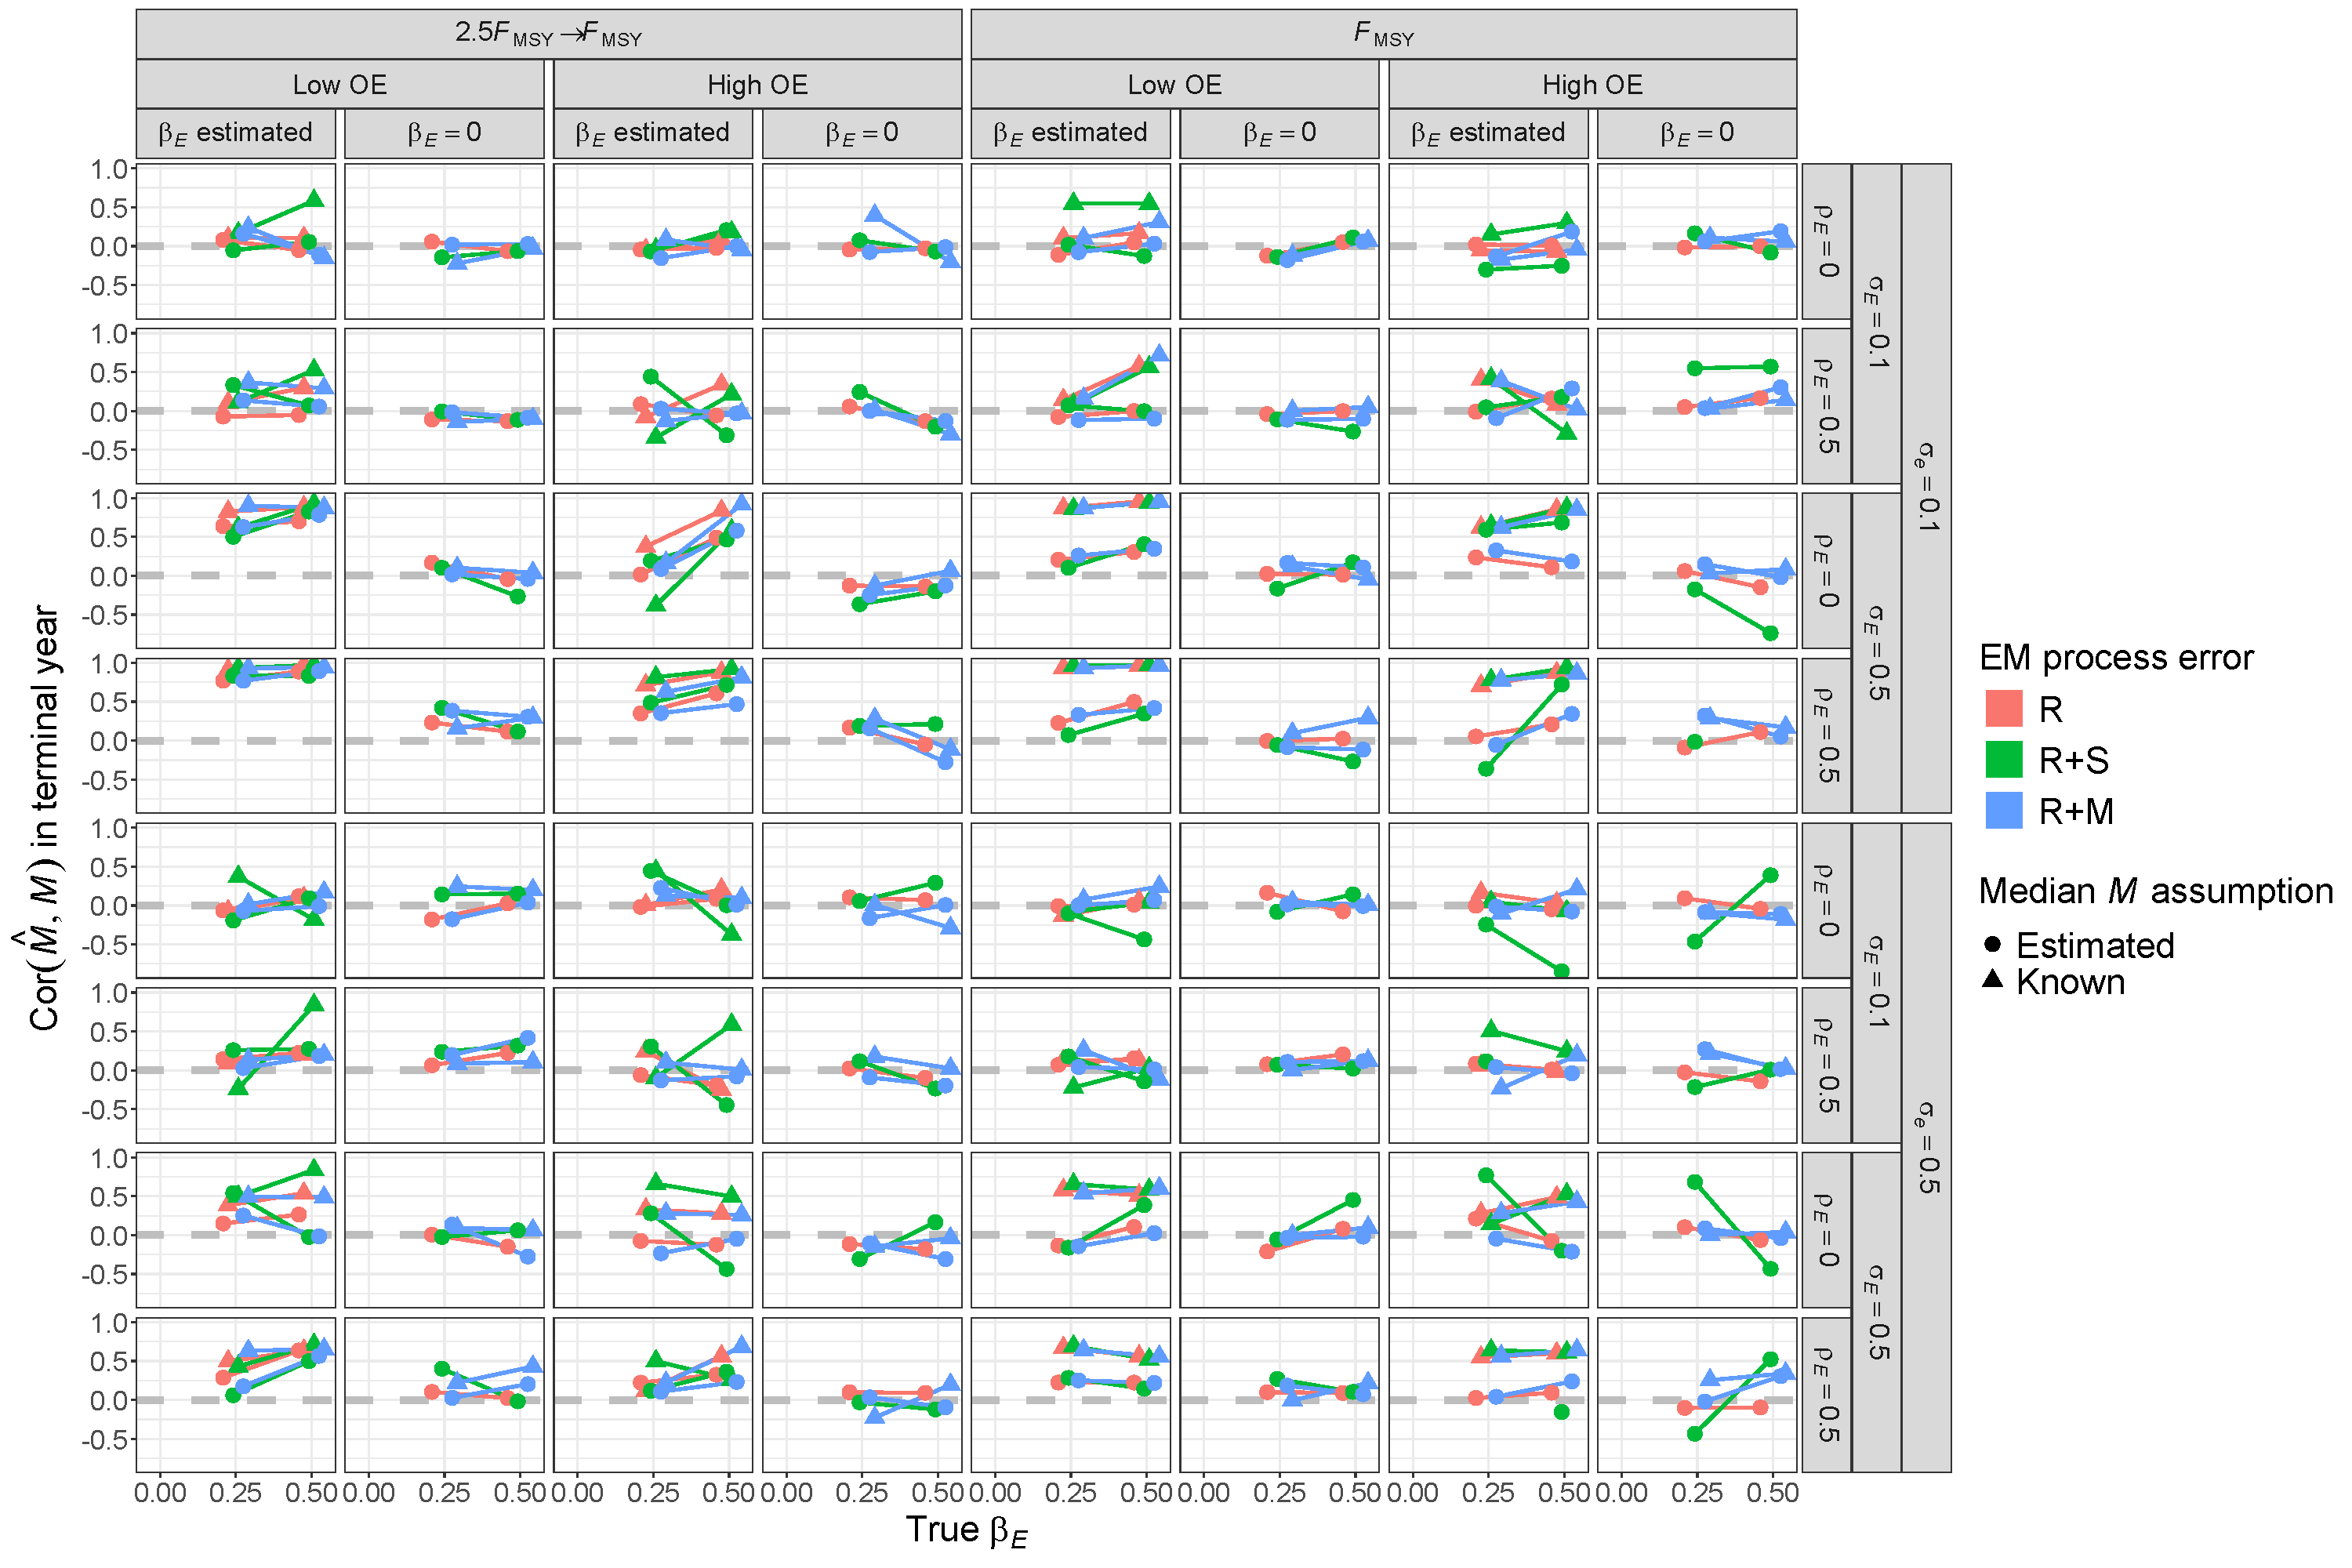
\includegraphics[height = \textheight]{terminal_year_M_corr_Rom}
\end{center}
\caption{For R operating models, correlation of estimates and true values of terminal year $M$ for estimating models with alternative process error assumptions, treatment of covariate effect ($\beta_E = 0$ or estimated), and treatment of median $M$ parameter ($\beta_M$ estimated or known).}\label{terminal_M_corr_Rom}
\end{figure}
\end{landscape}

\begin{landscape}
\begin{figure}
\begin{center}
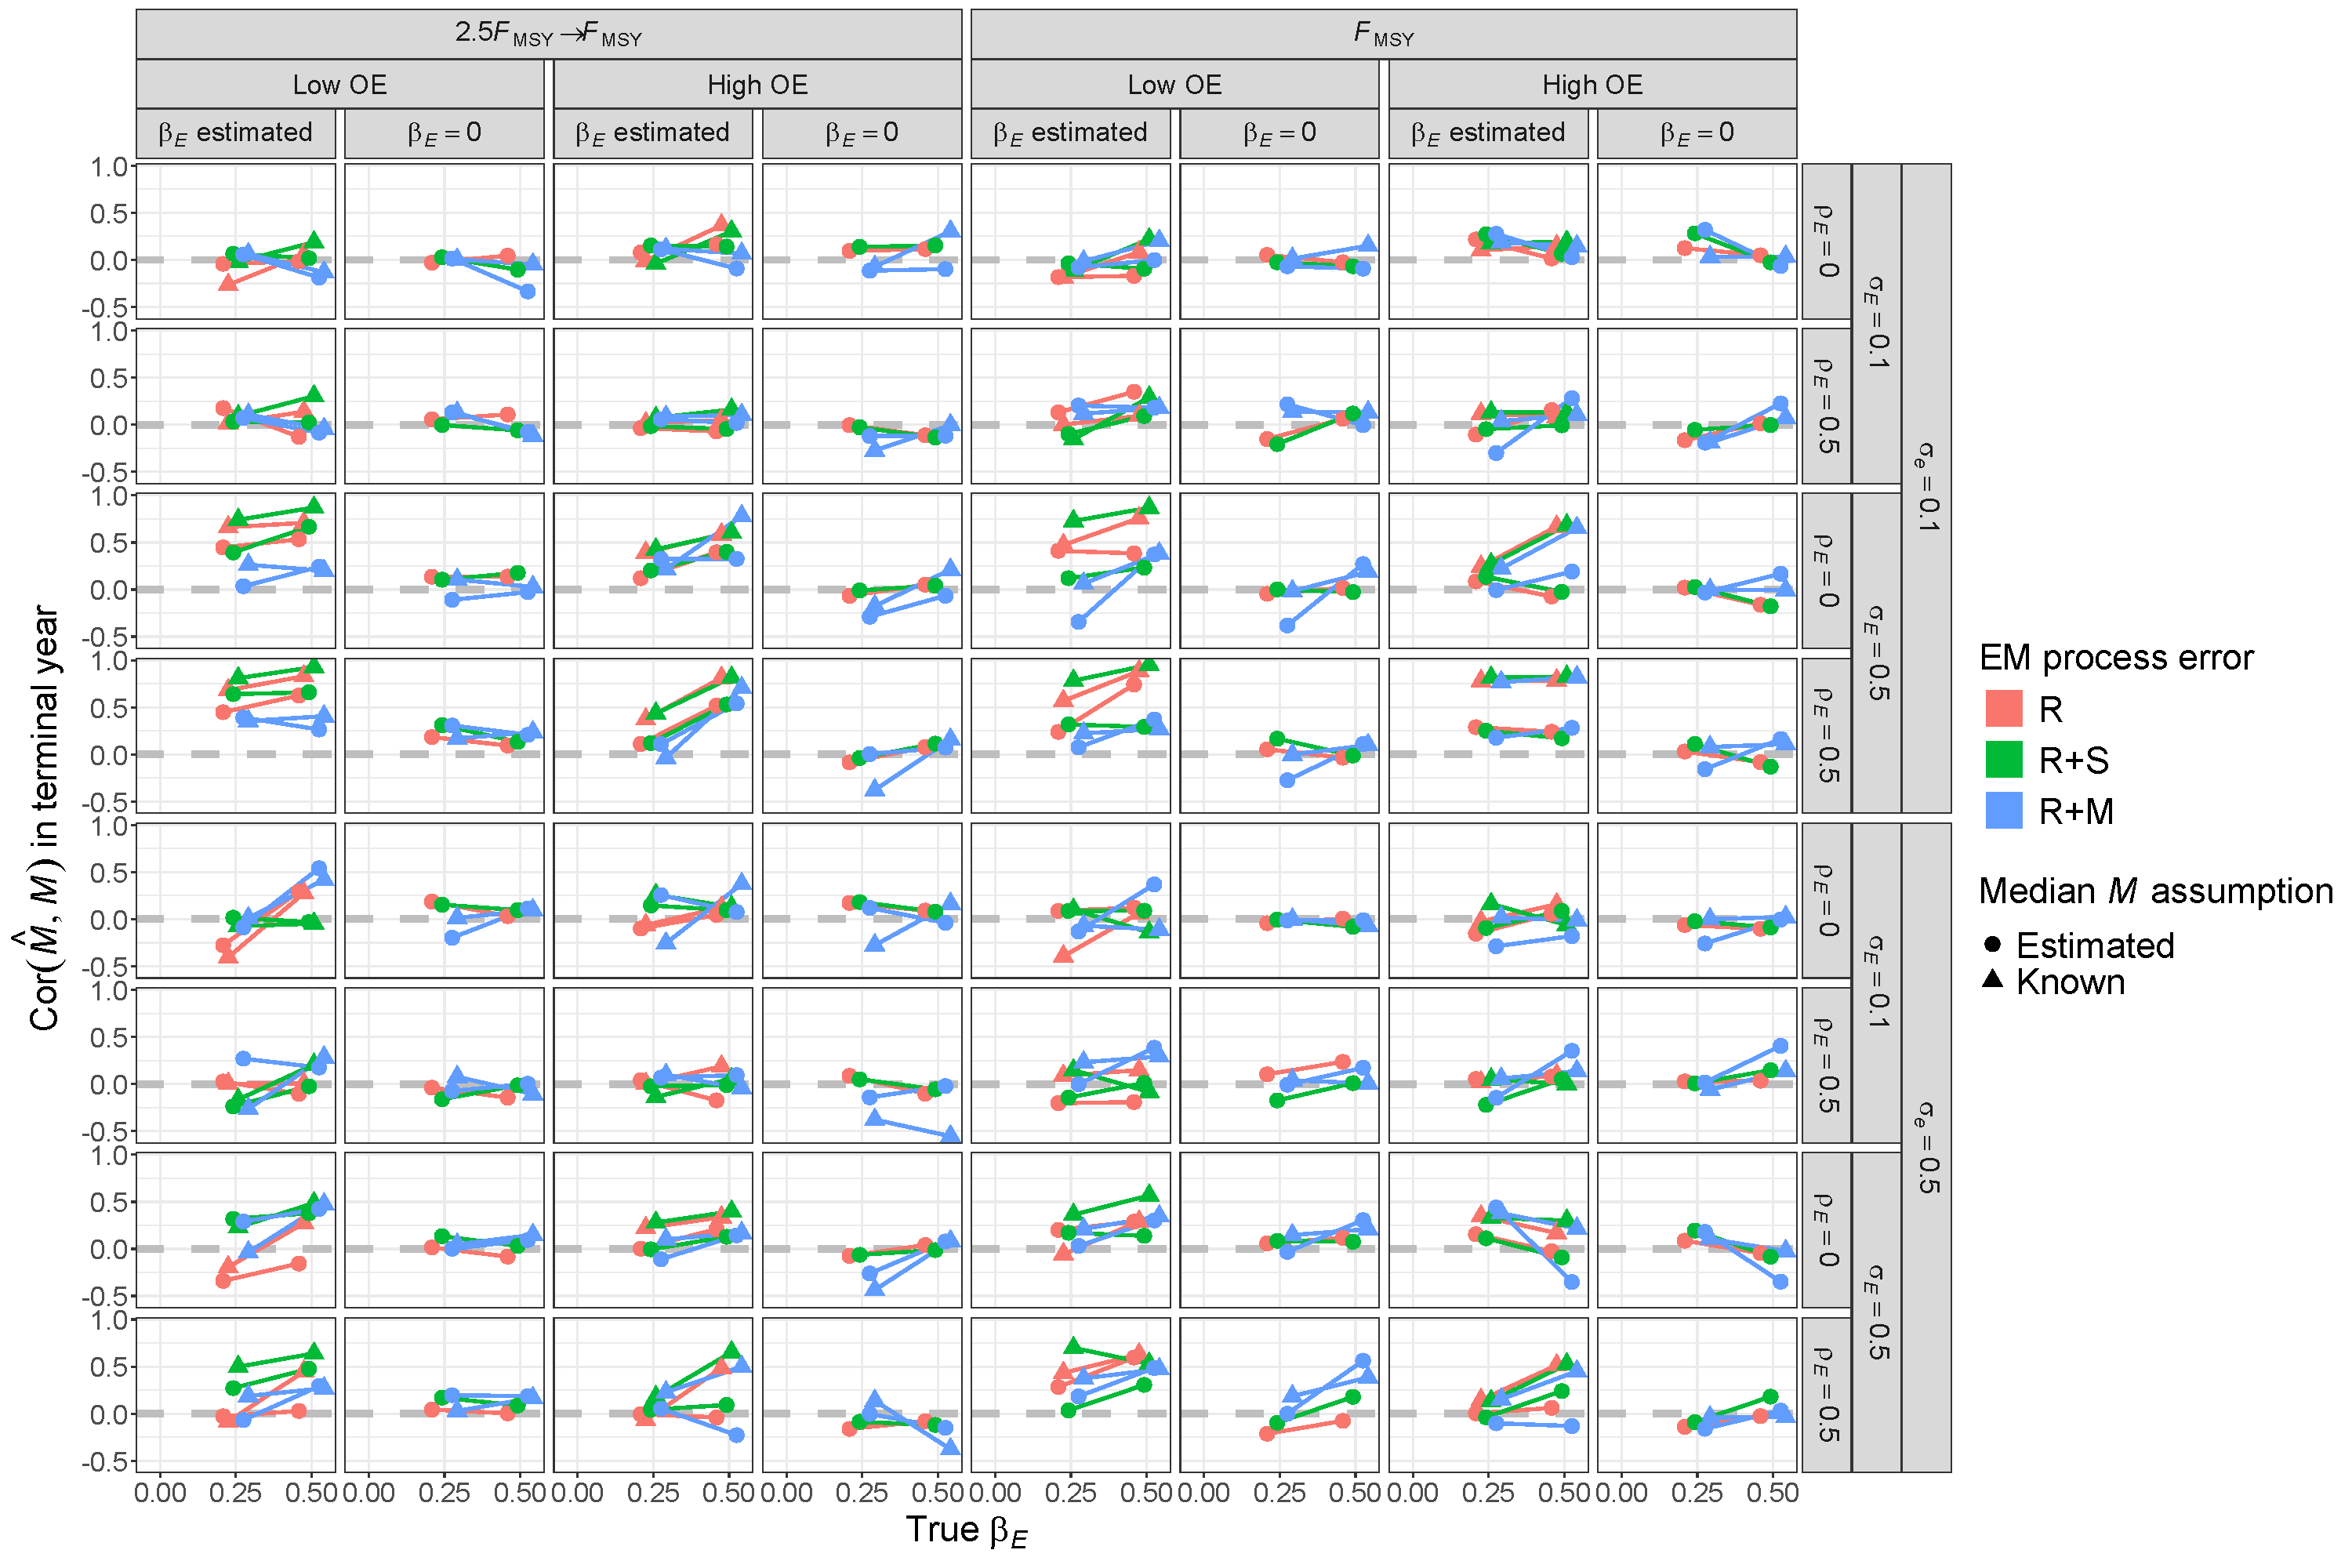
\includegraphics[height = \textheight]{terminal_year_M_corr_RSom}
\end{center}
\caption{For R+S operating models, correlation of estimates and true values of terminal year $M$ for estimating models with alternative process error assumptions, treatment of covariate effect ($\beta_E = 0$ or estimated), and treatment of median $M$ parameter ($\beta_M$ estimated or known).}\label{terminal_M_corr_RSom}
\end{figure}
\end{landscape}

\begin{landscape}
\begin{figure}
\begin{center}
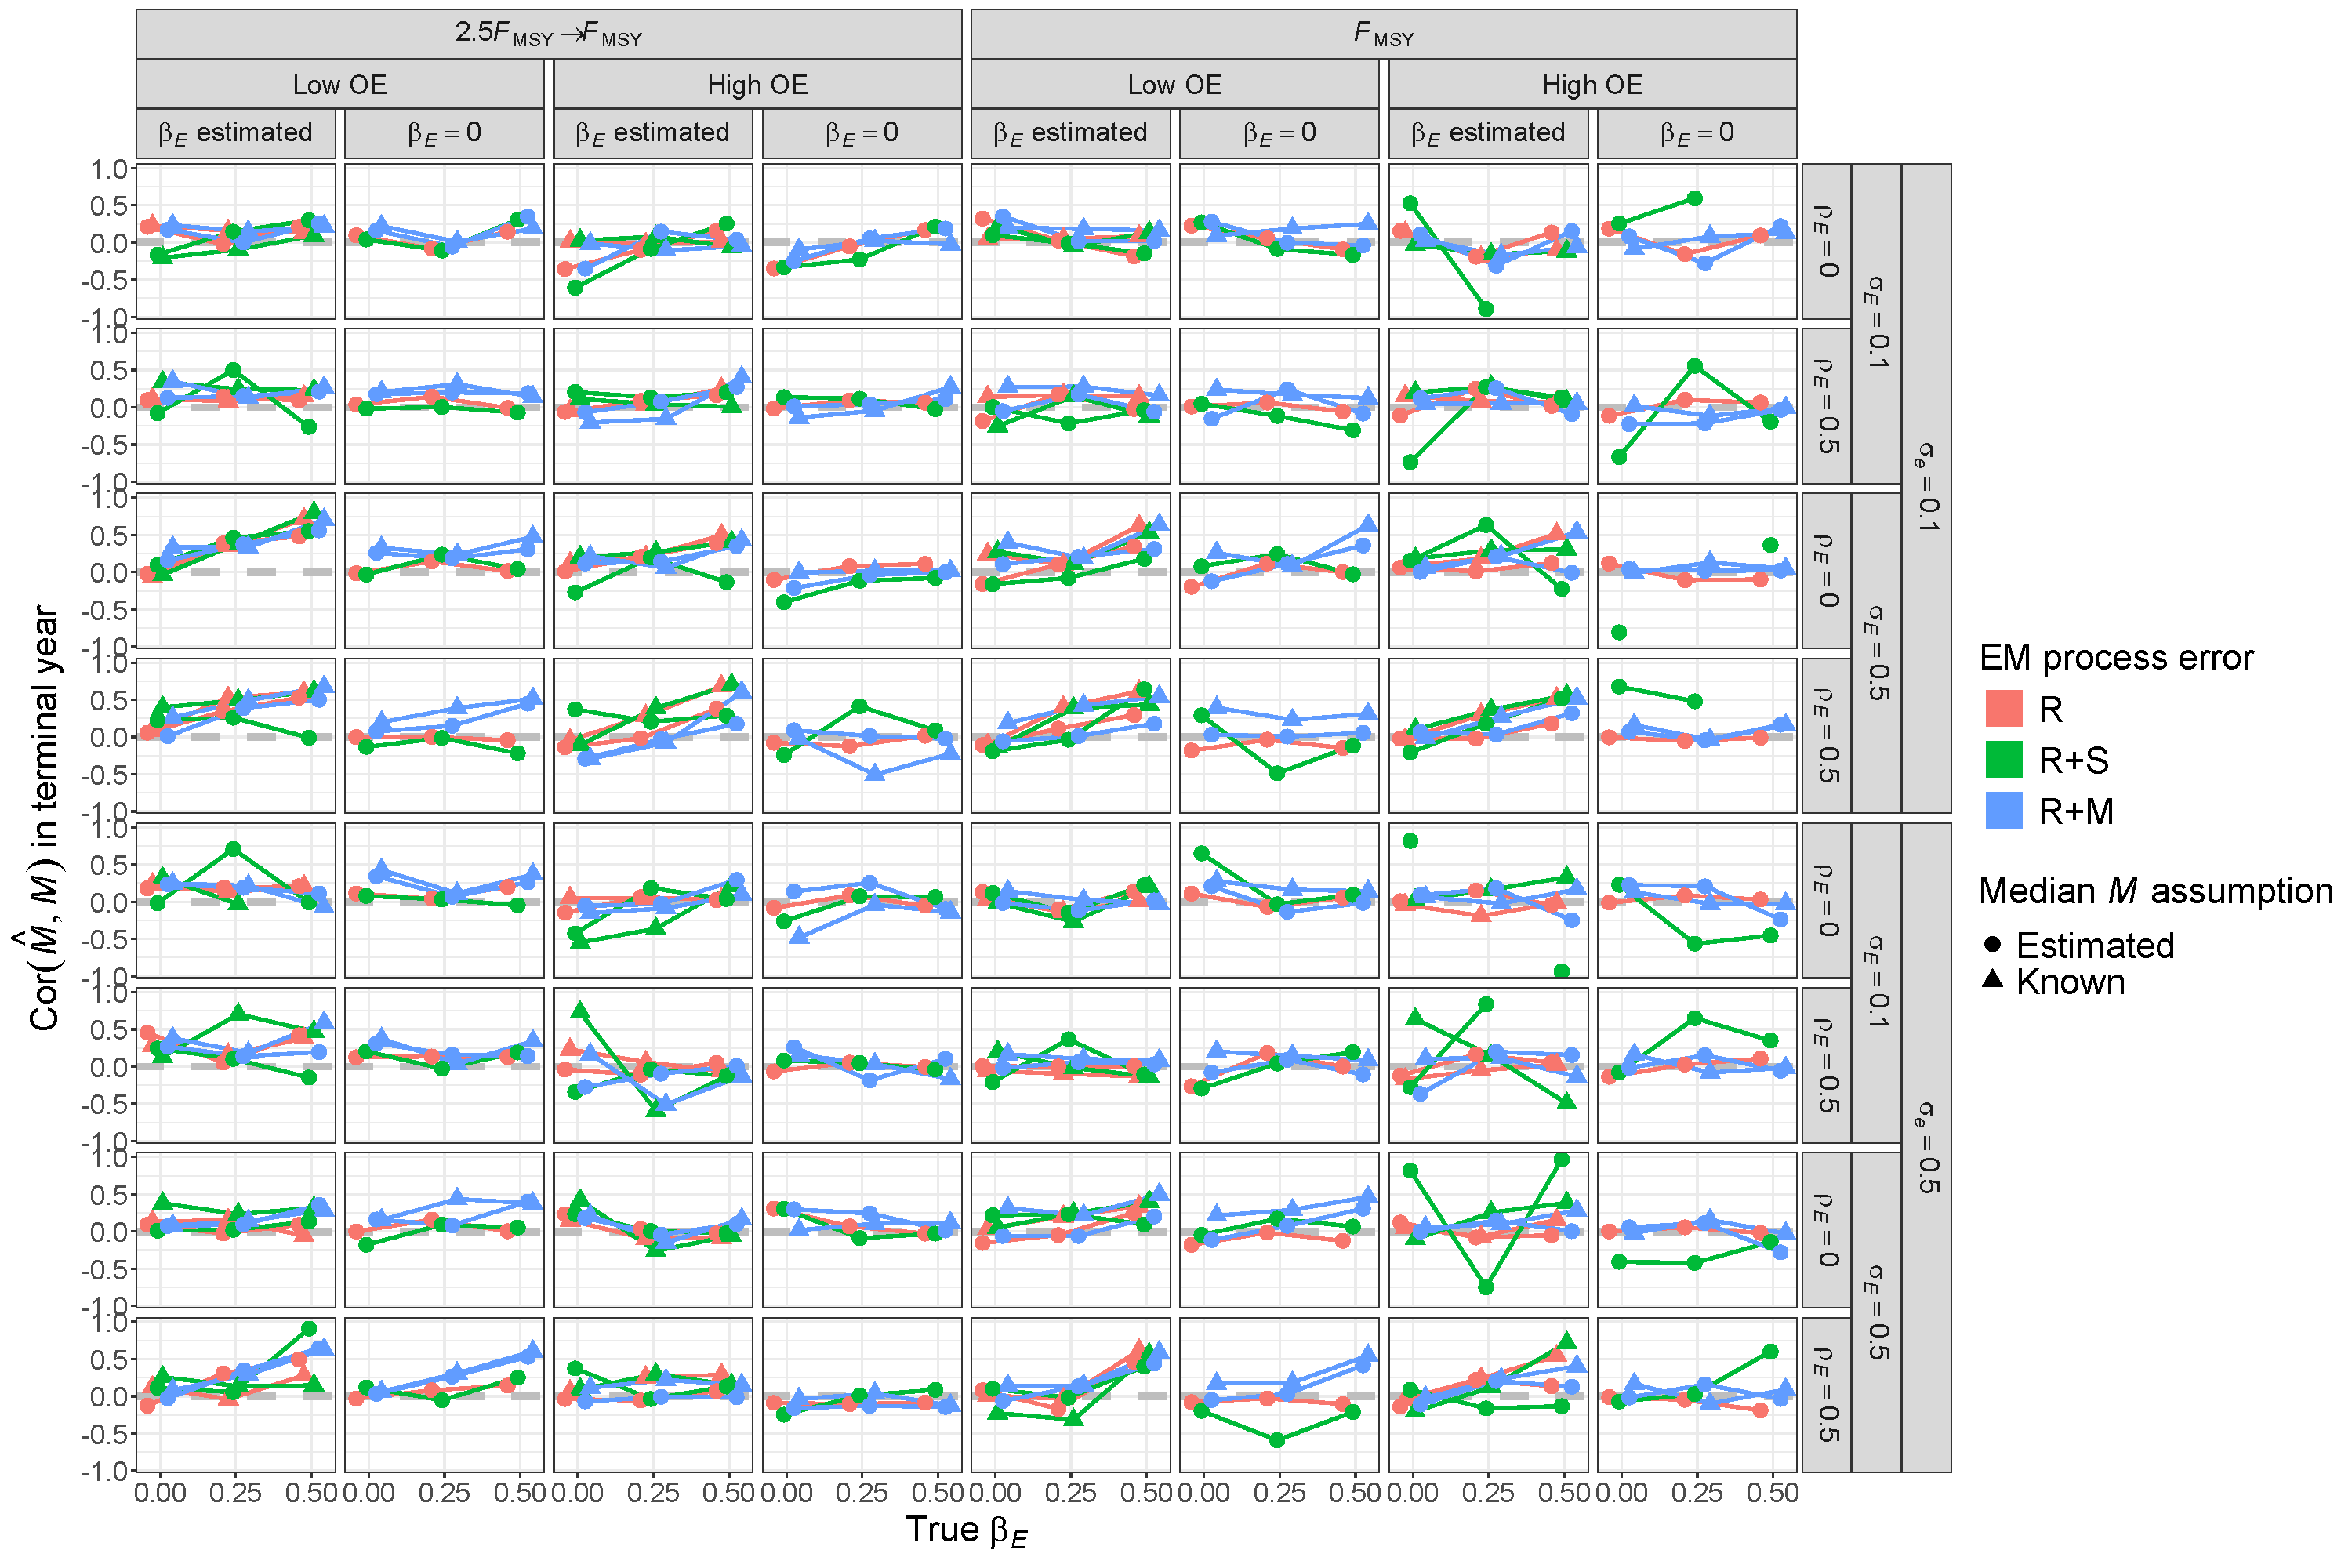
\includegraphics[height = \textheight]{terminal_year_M_corr_RMom}
\end{center}
\caption{For R+M operating models, correlation of estimates and true vales of terminal year $M$ for estimating models with alternative process error assumptions, treatment of covariate effect ($\beta_E = 0$ or estimated), and treatment of median $M$ parameter ($\beta_M$ estimated or known).}\label{terminal_M_corr_RMom}
\end{figure}
\end{landscape}

\begin{landscape}
\begin{figure}
\begin{center}
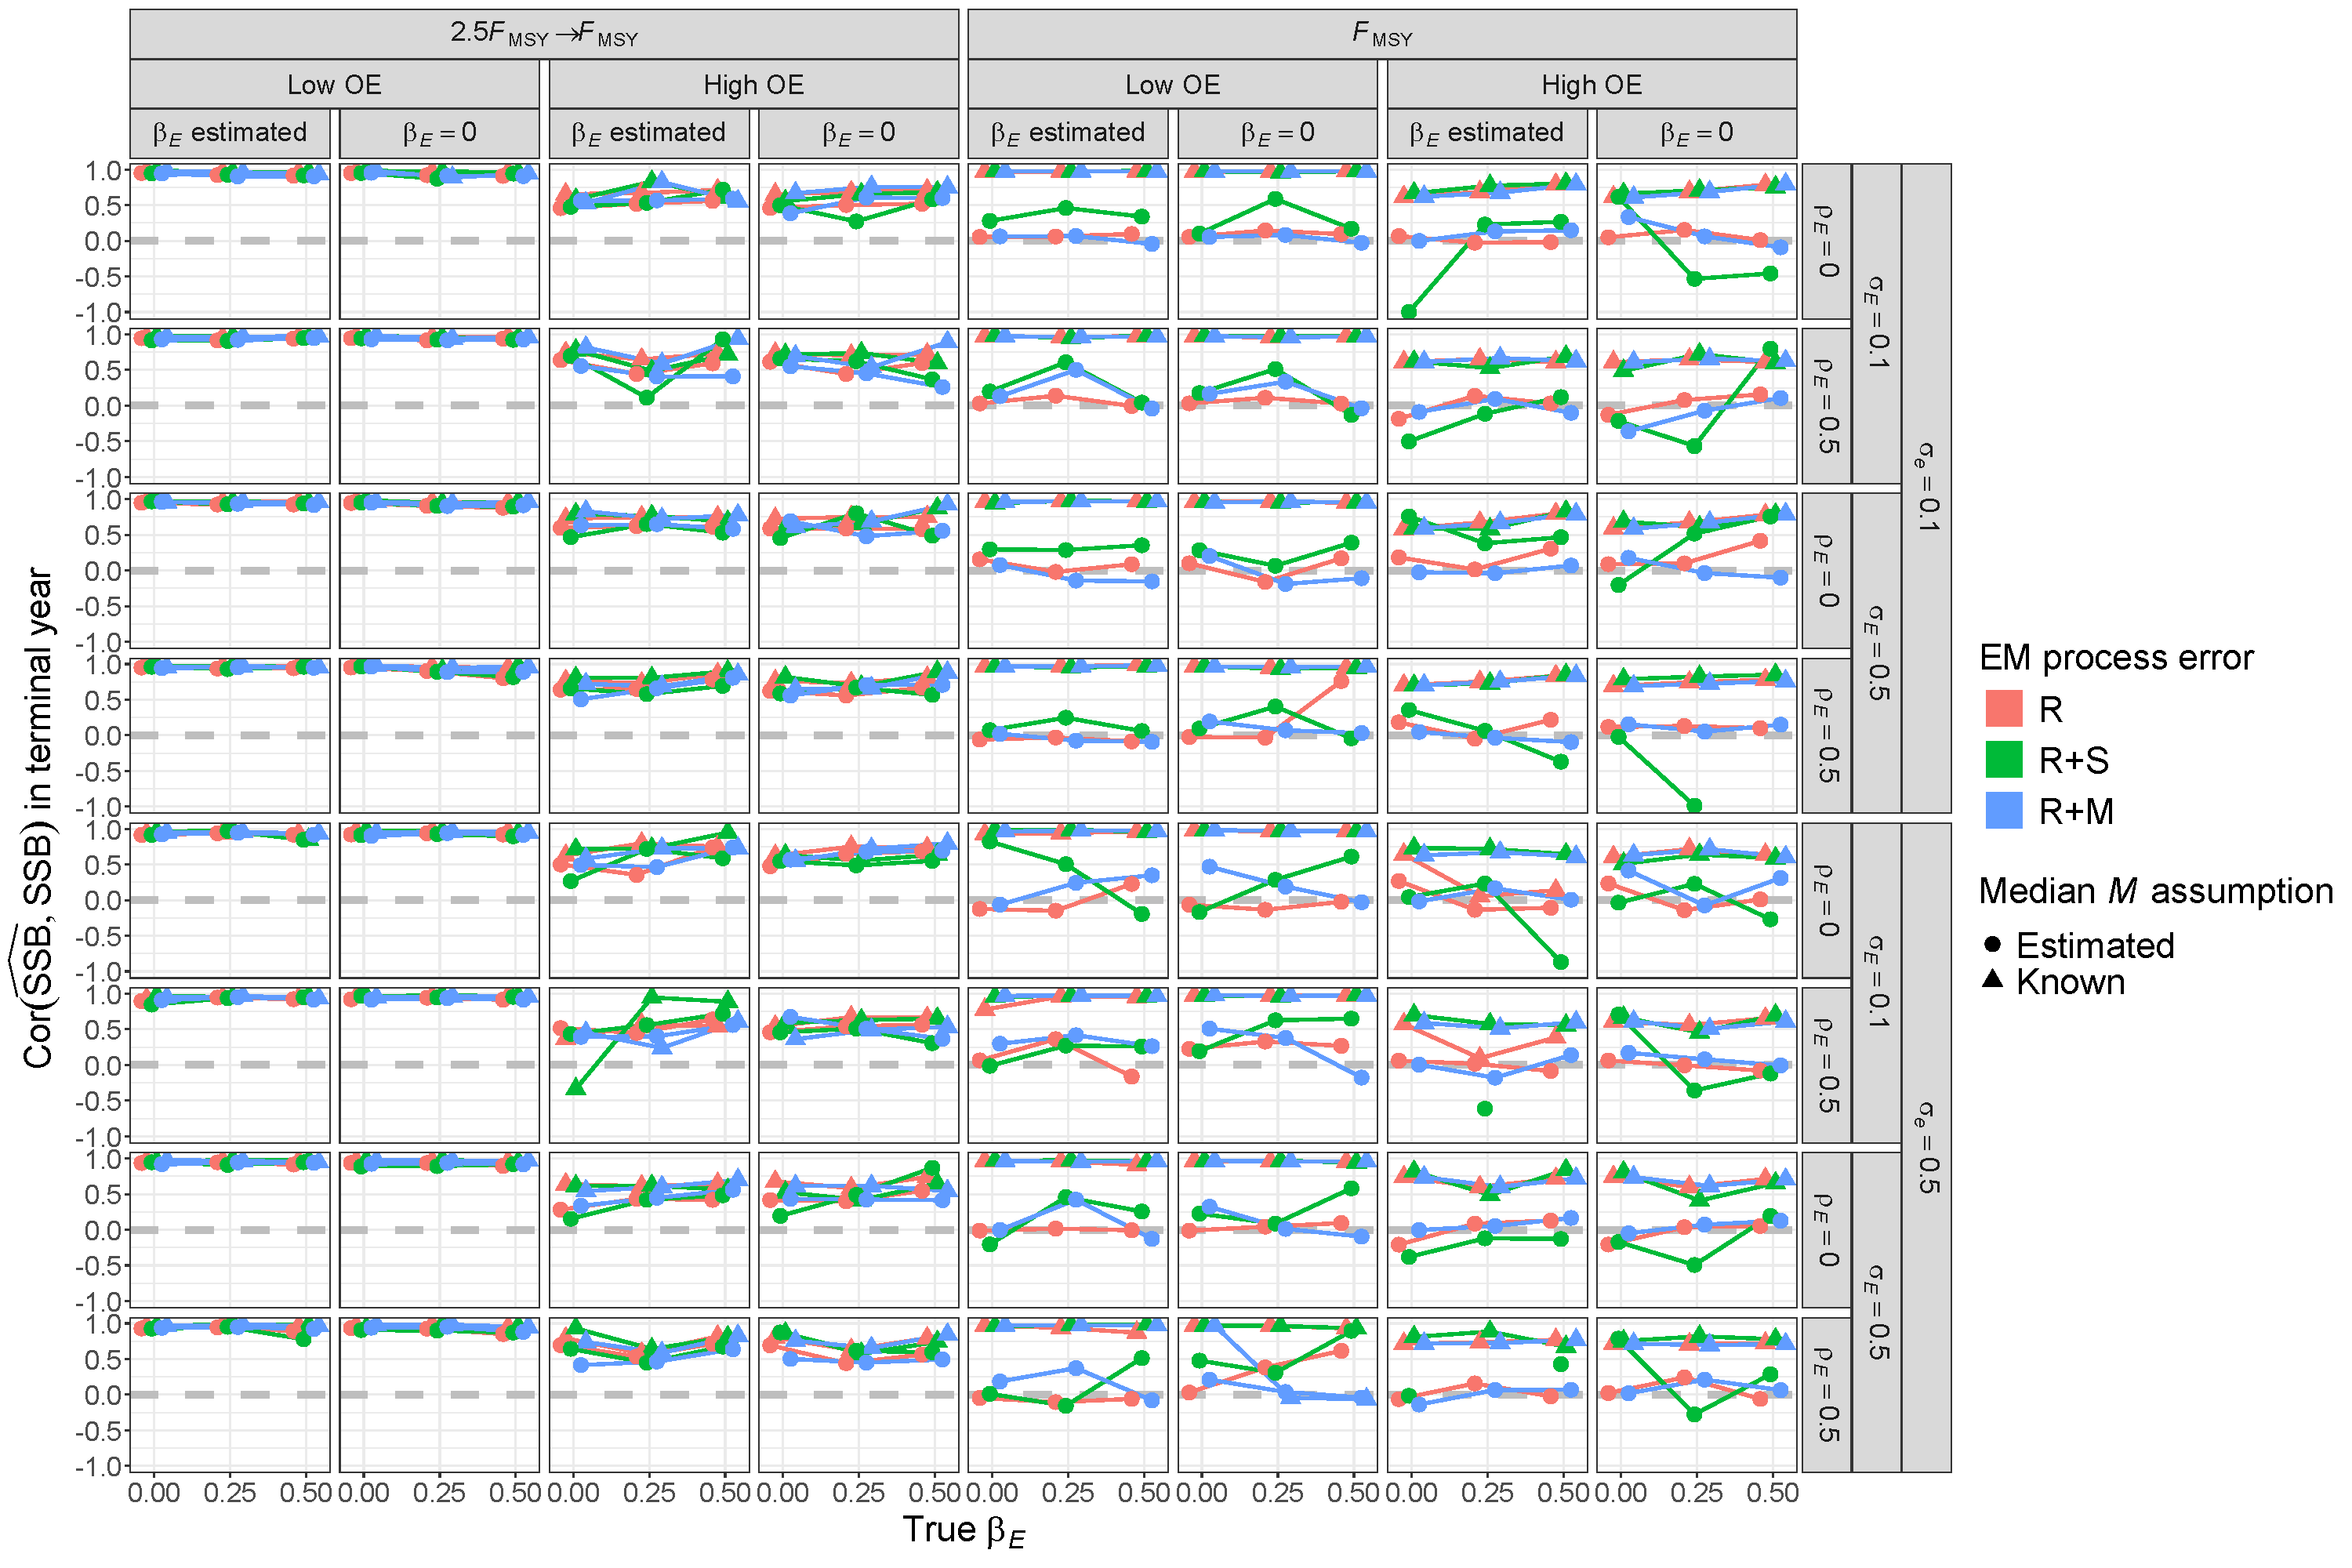
\includegraphics[height = \textheight]{terminal_year_ssb_corr_Rom}
\end{center}
\caption{For R operating models, correlation of estimates and true values of terminal year SSB for estimating models with alternative process error assumptions, treatment of covariate effect ($\beta_E = 0$ or estimated), and treatment of median $M$ parameter ($\beta_M$ estimated or known).}\label{terminal_ssb_corr_Rom}
\end{figure}
\end{landscape}

\begin{landscape}
\begin{figure}
\begin{center}
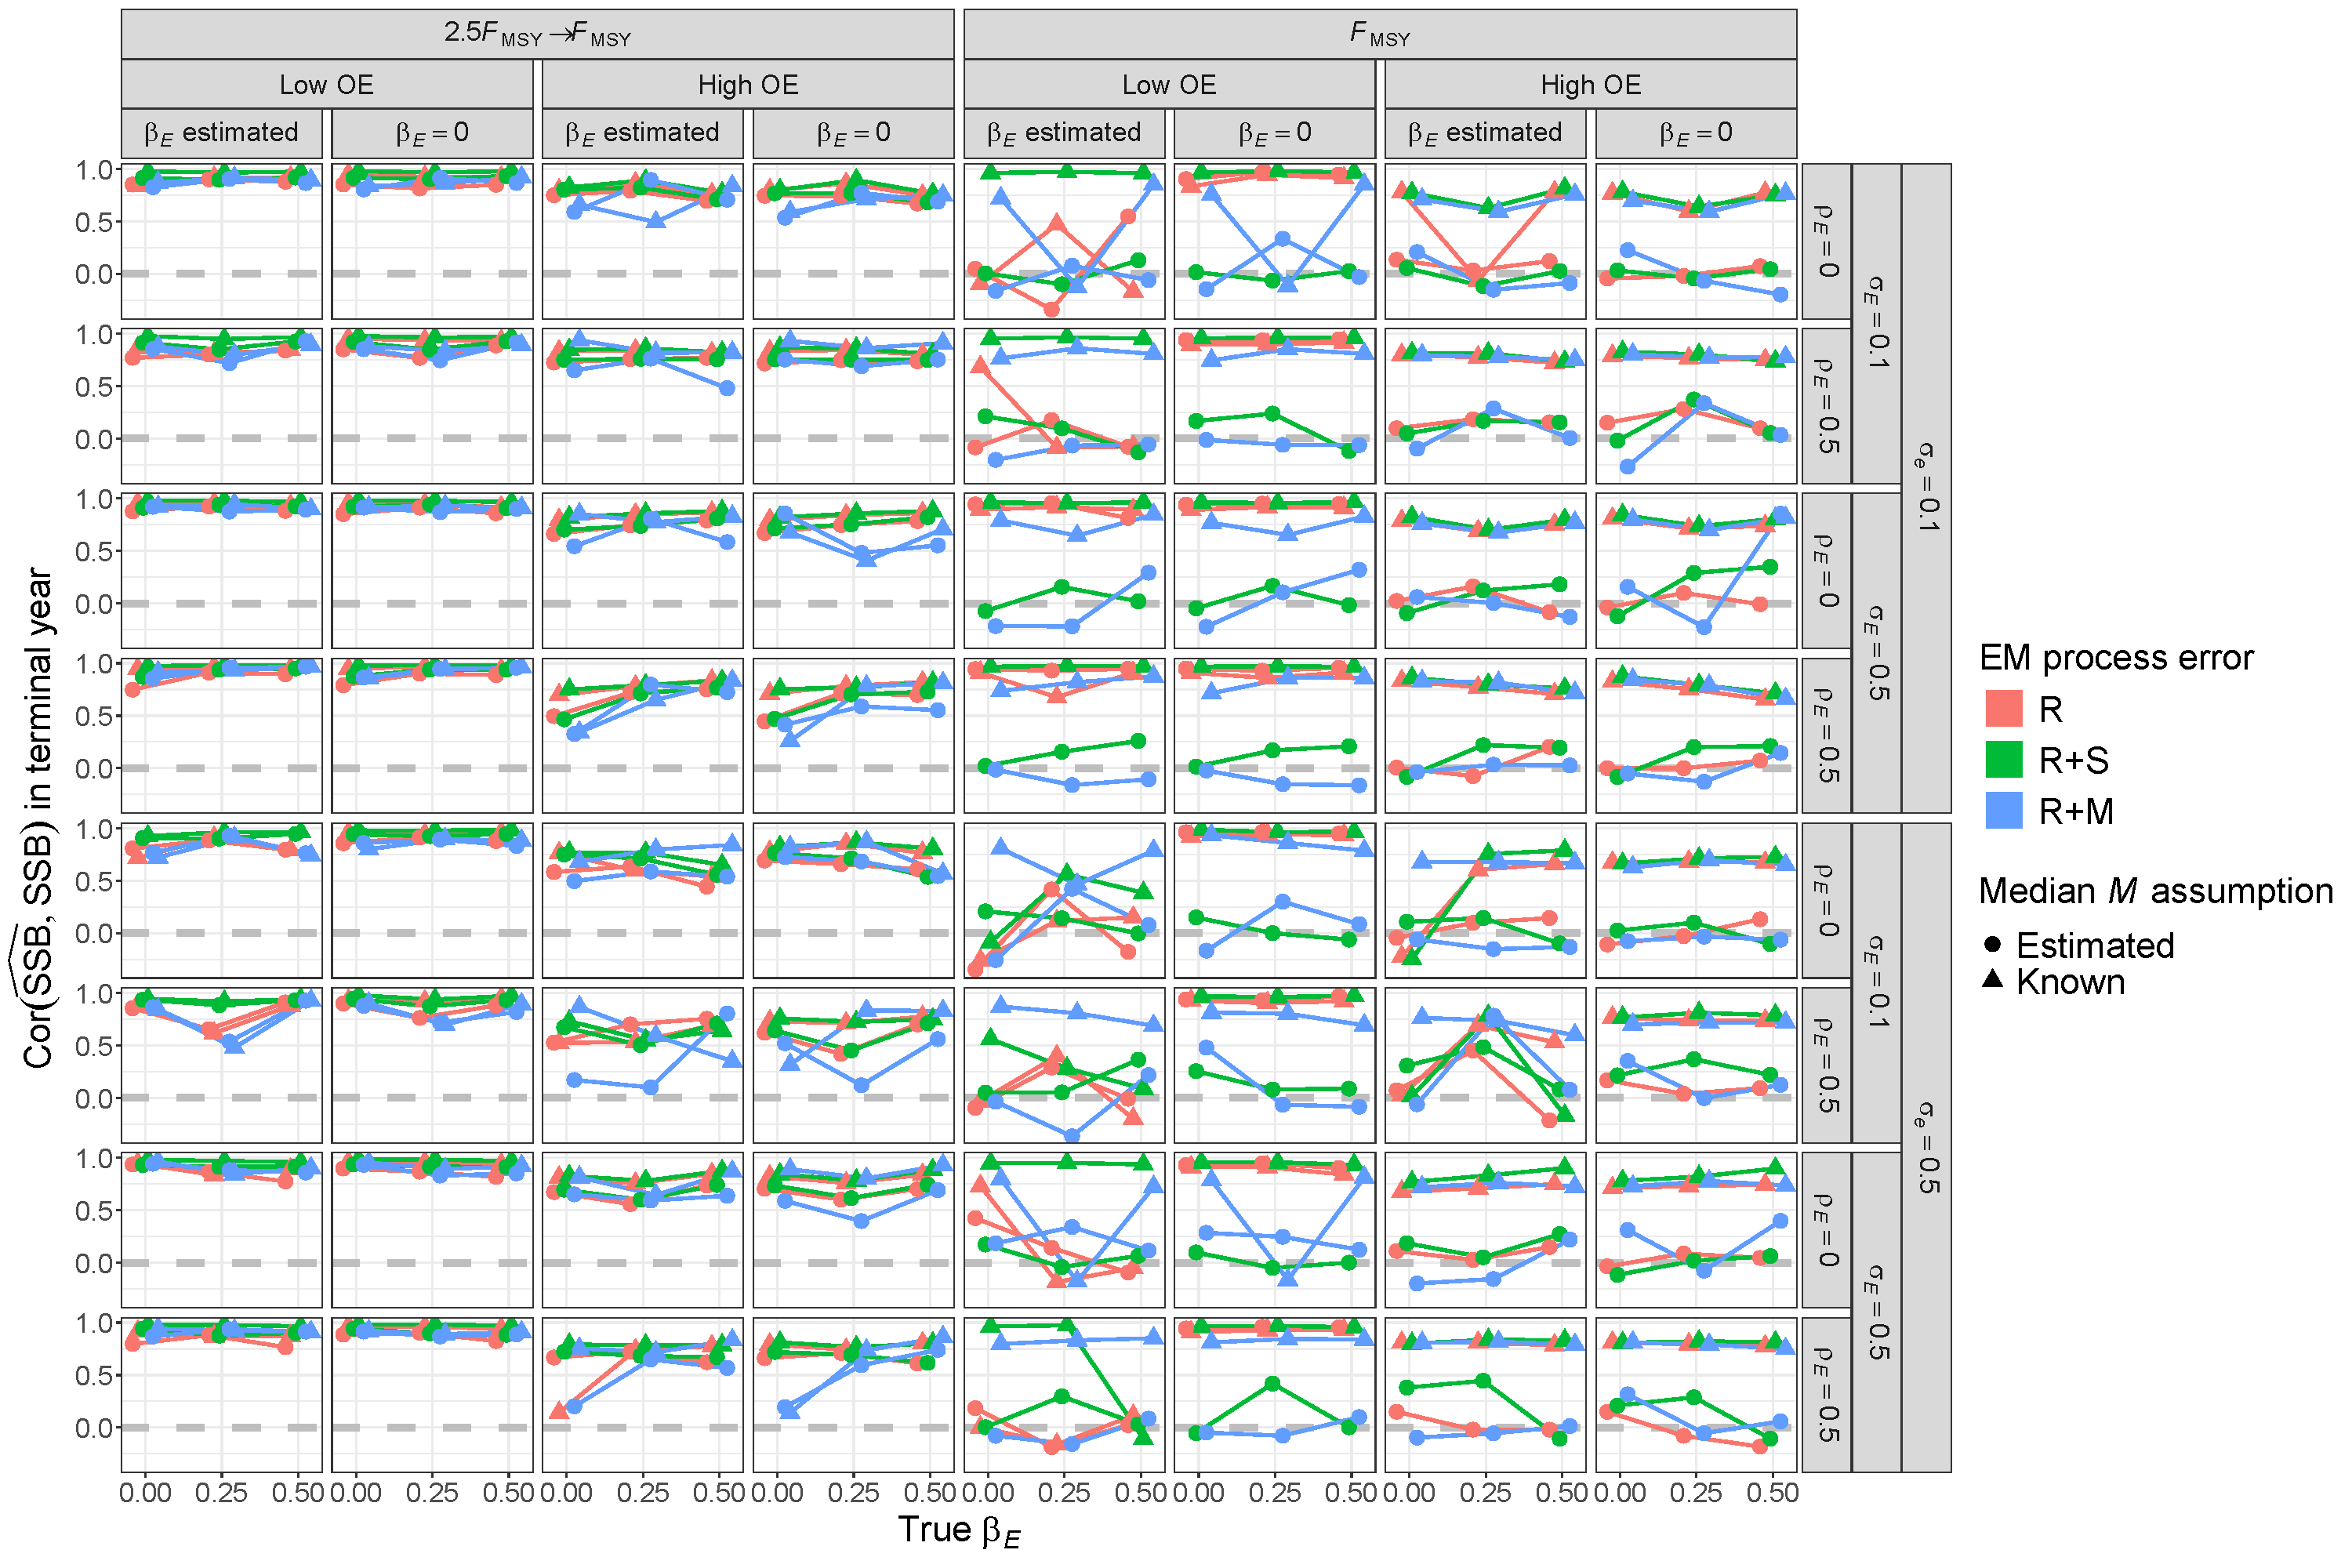
\includegraphics[height = \textheight]{terminal_year_ssb_corr_RSom}
\end{center}
\caption{For R+S operating models, correlation of estimates and true values of terminal year SSB for estimating models with alternative process error assumptions, treatment of covariate effect ($\beta_E = 0$ or estimated), and treatment of median $M$ parameter ($\beta_M$ estimated or known).}\label{terminal_ssb_corr_RSom}
\end{figure}
\end{landscape}

\begin{landscape}
\begin{figure}
\begin{center}
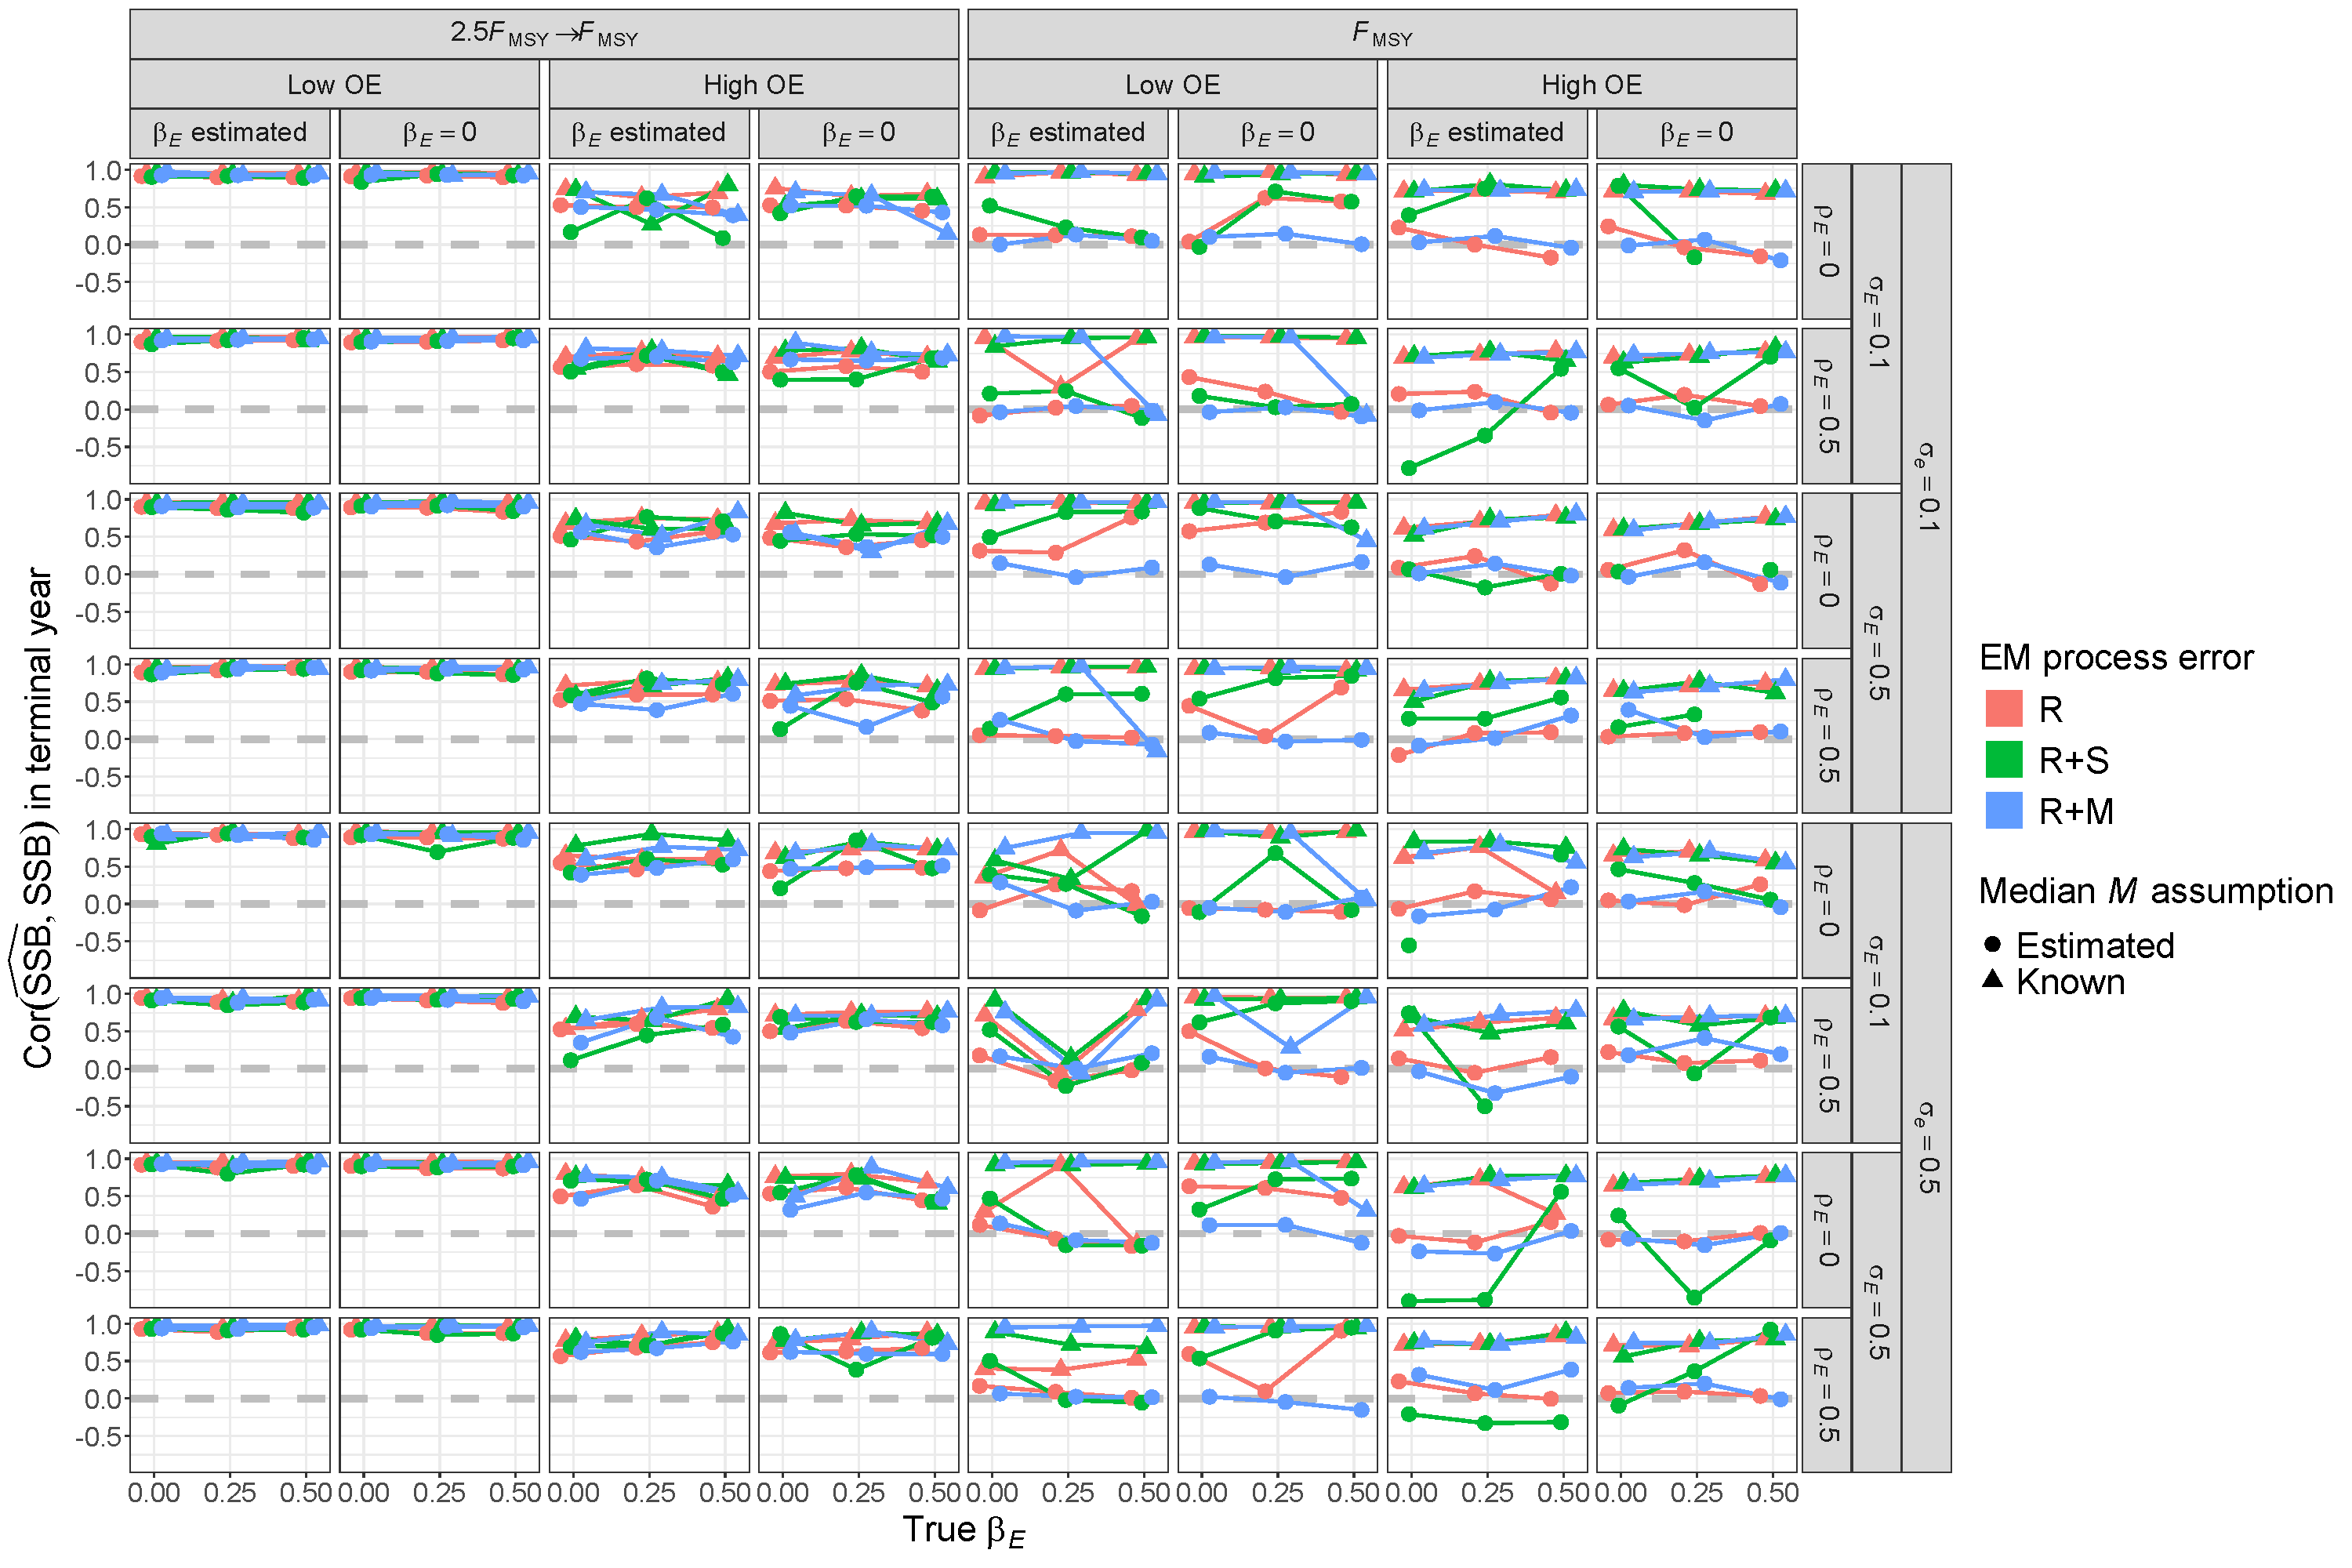
\includegraphics[height = \textheight]{terminal_year_ssb_corr_RMom}
\end{center}
\caption{For R+M operating models, correlation of estimates and true vales of terminal year SSB for estimating models with alternative process error assumptions, treatment of covariate effect ($\beta_E = 0$ or estimated), and treatment of median $M$ parameter ($\beta_M$ estimated or known).}\label{terminal_ssb_corr_RMom}
\end{figure}
\end{landscape}

\begin{landscape}
\begin{figure}
\begin{center}
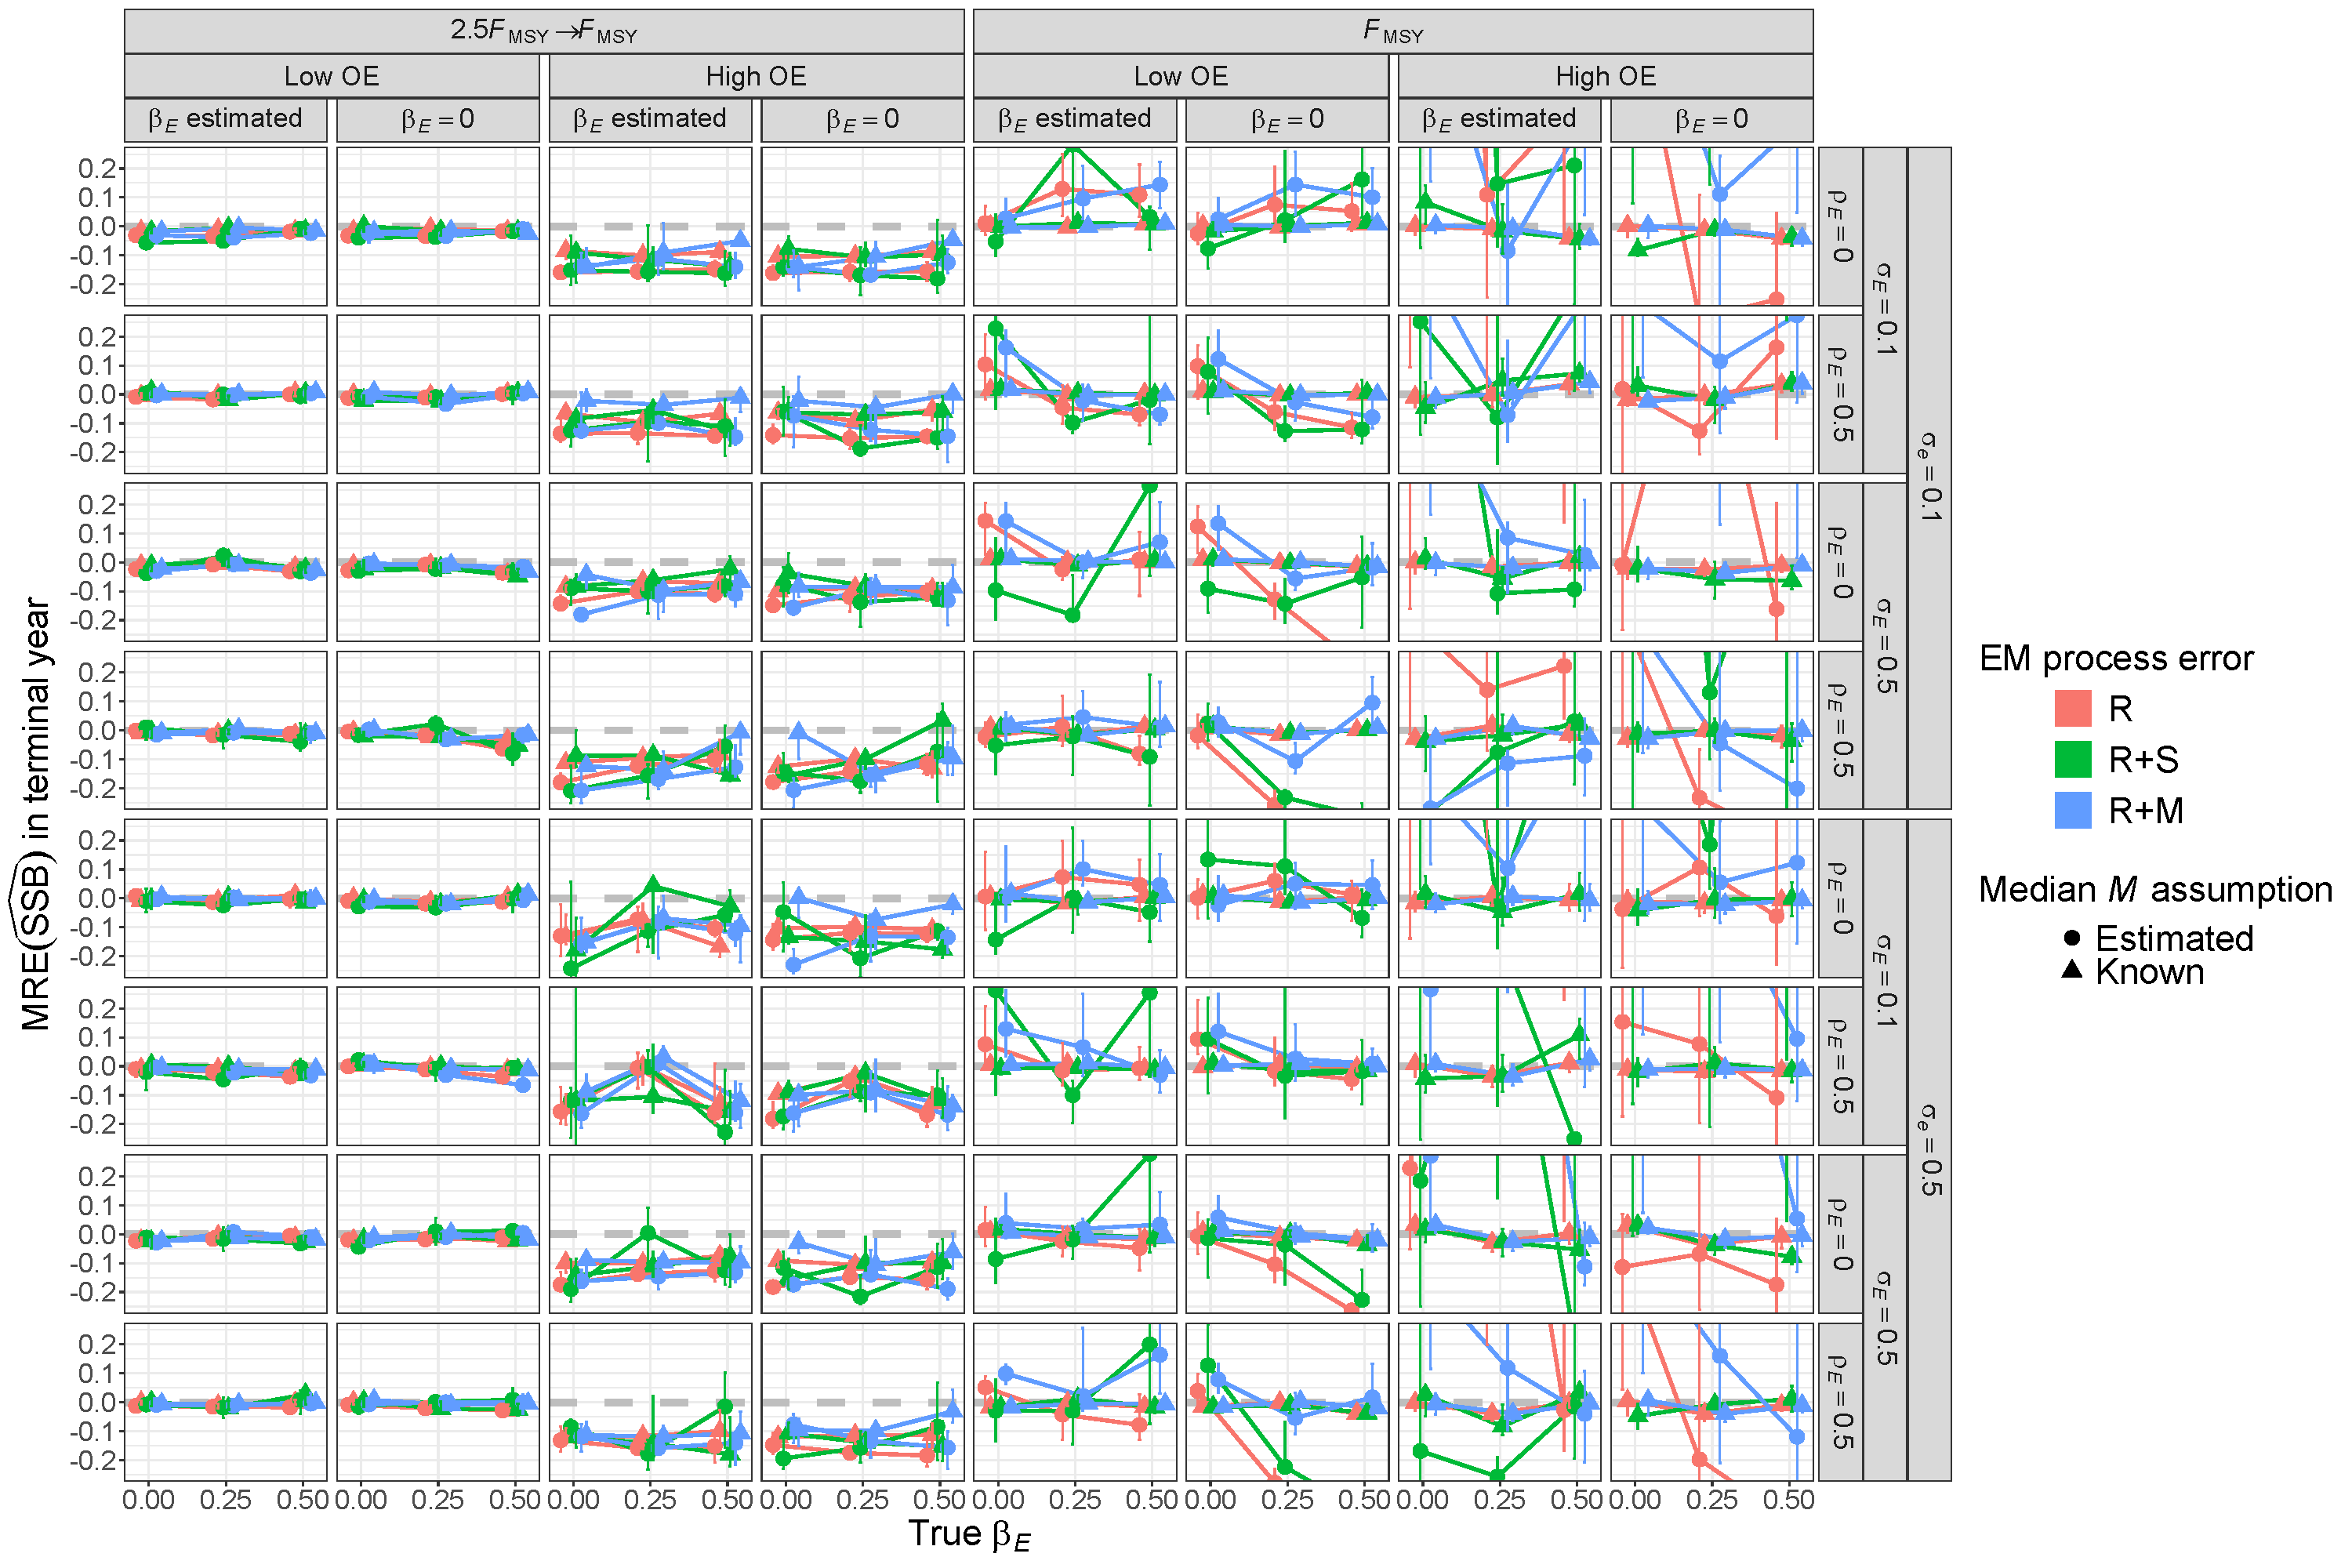
\includegraphics[height = \textheight]{terminal_year_ssb_bias_Rom}
\end{center}
\caption{For R operating models, median relative error (MRE) of estimates of SSB in the terminal year for estimating models with alternative process error assumptions, treatment of covariate effect ($\beta_E = 0$ or estimated), and treatment of median $M$ parameter ($\beta_M$ estimated or known).}\label{terminal_ssb_bias_Rom}
\end{figure}
\end{landscape}

\begin{landscape}
\begin{figure}
\begin{center}
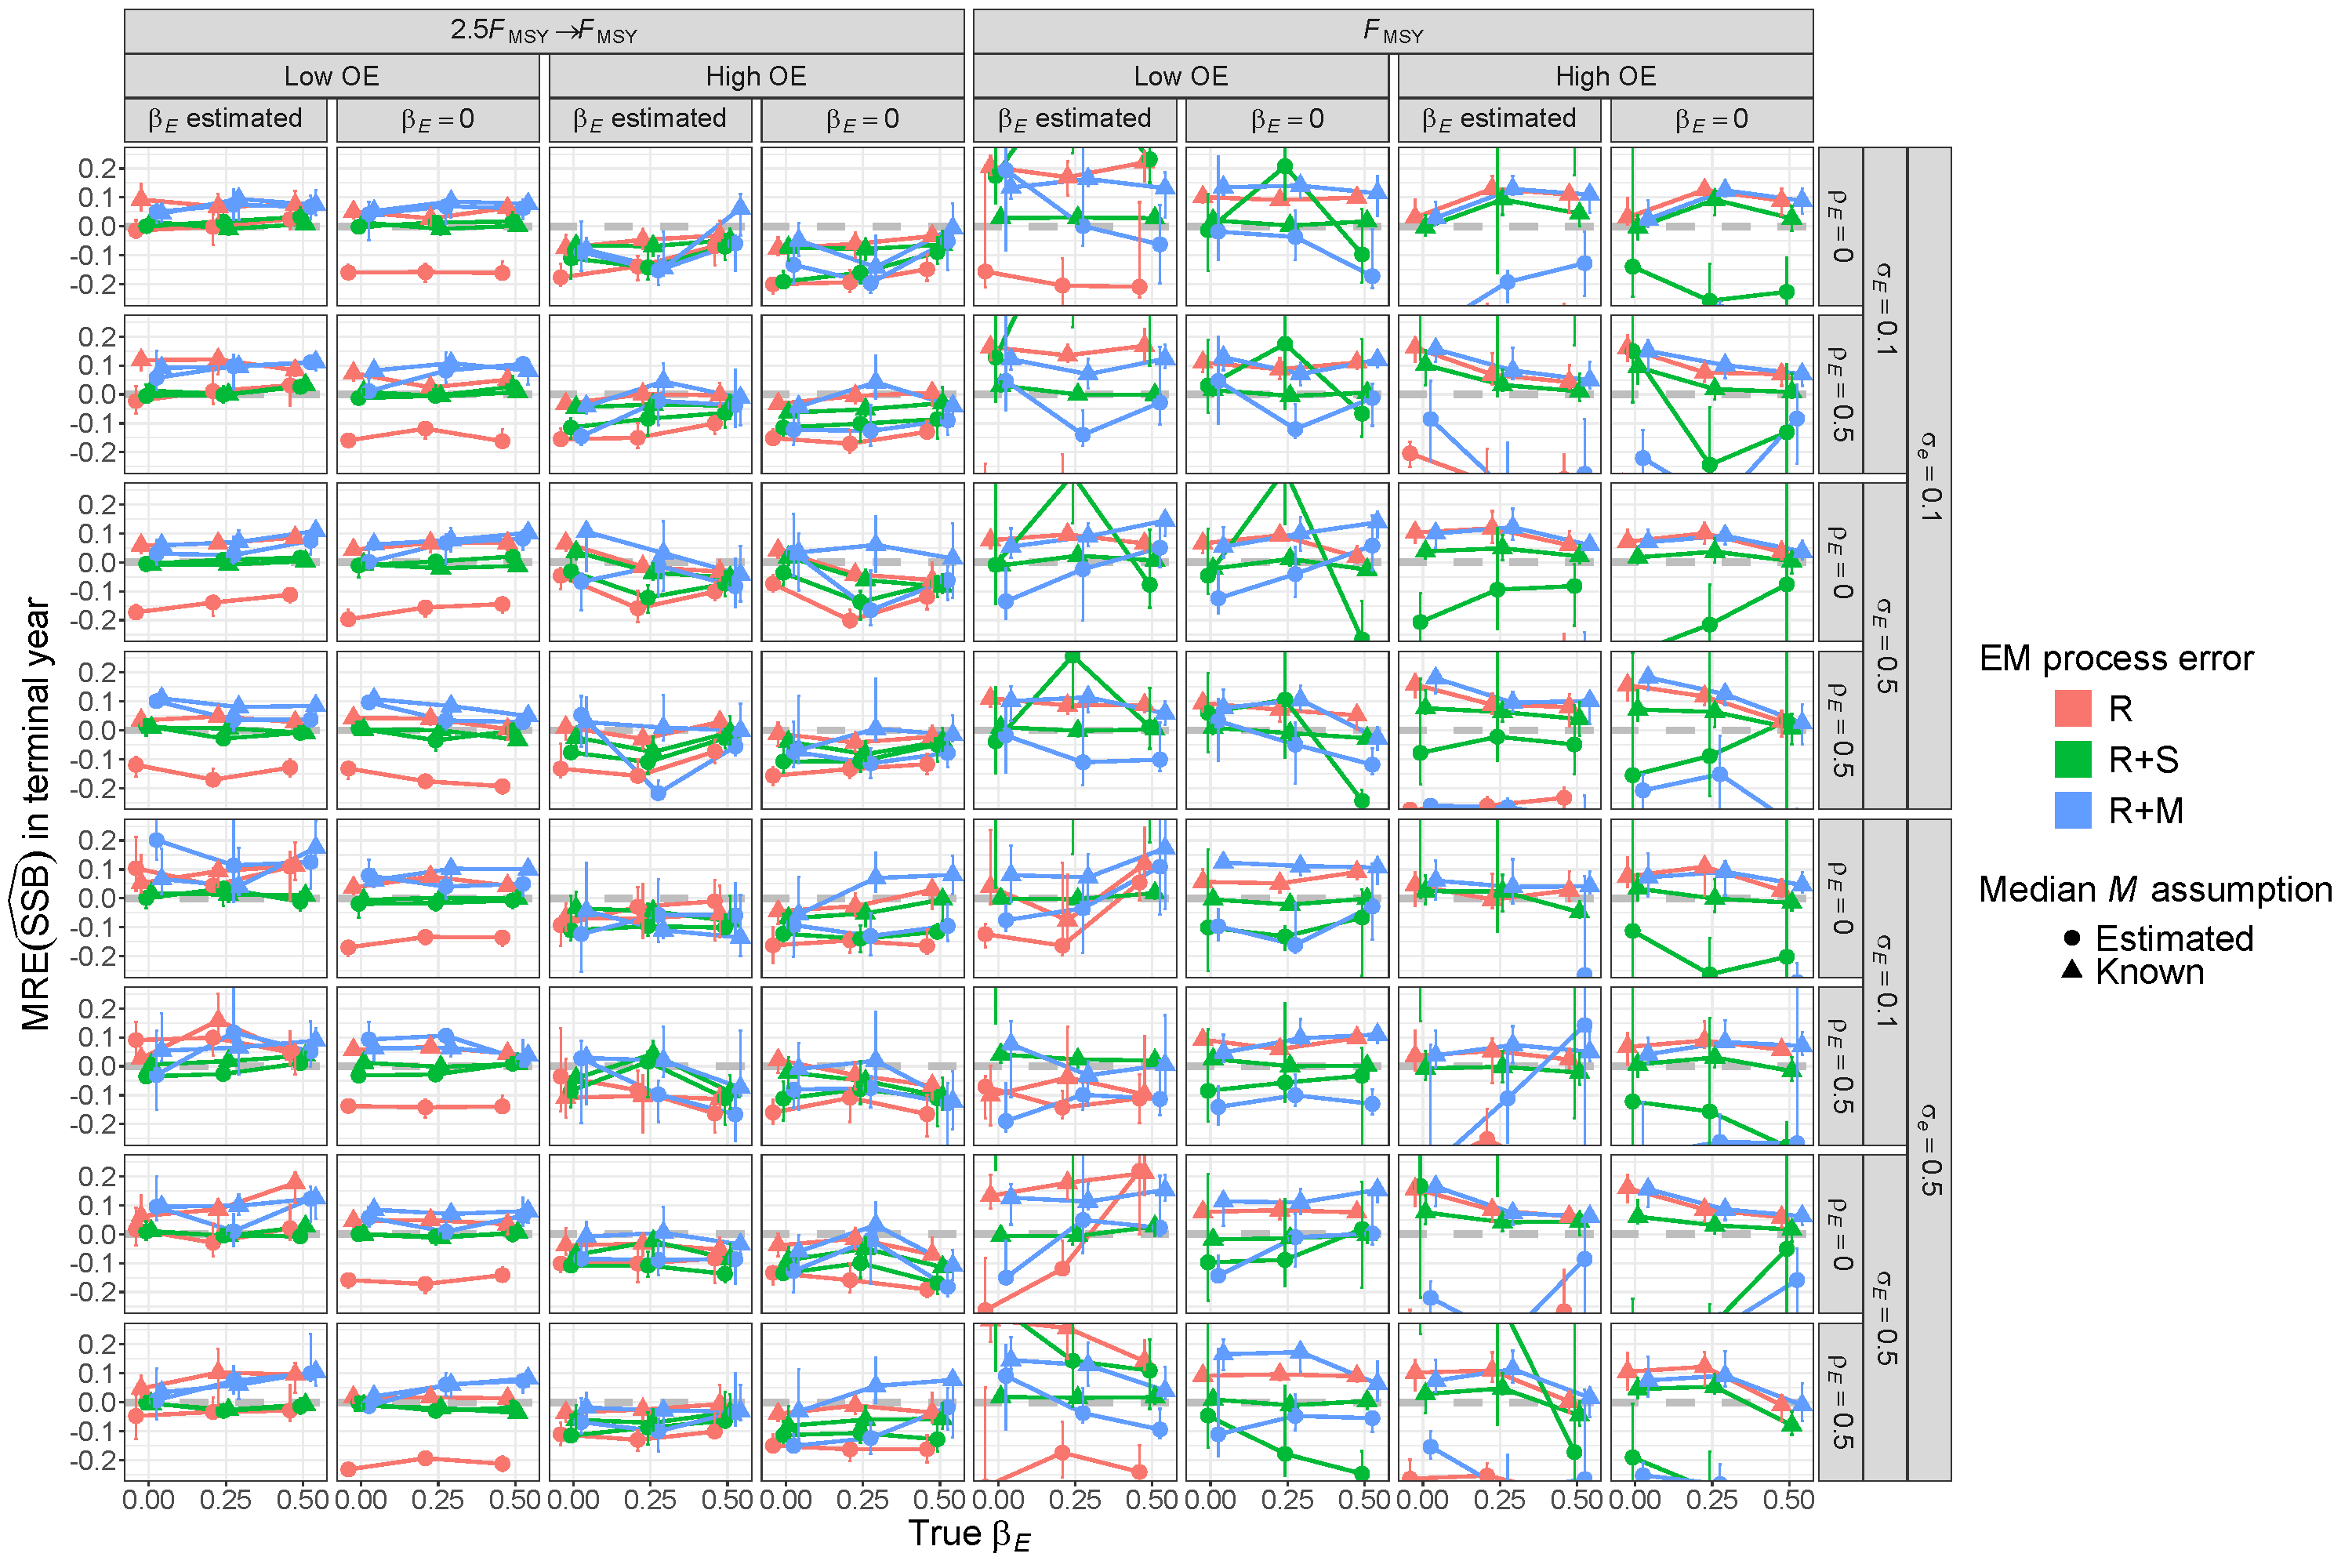
\includegraphics[height = \textheight]{terminal_year_ssb_bias_RSom}
\end{center}
\caption{For R+S operating models, median relative error (MRE) of SSB in the terminal year for estimating models with alternative process error assumptions, treatment of covariate effect ($\beta_E = 0$ or estimated), and treatment of median $M$ parameter ($\beta_M$ estimated or known).}\label{terminal_ssb_bias_RSom}
\end{figure}
\end{landscape}

\begin{landscape}
\begin{figure}
\begin{center}
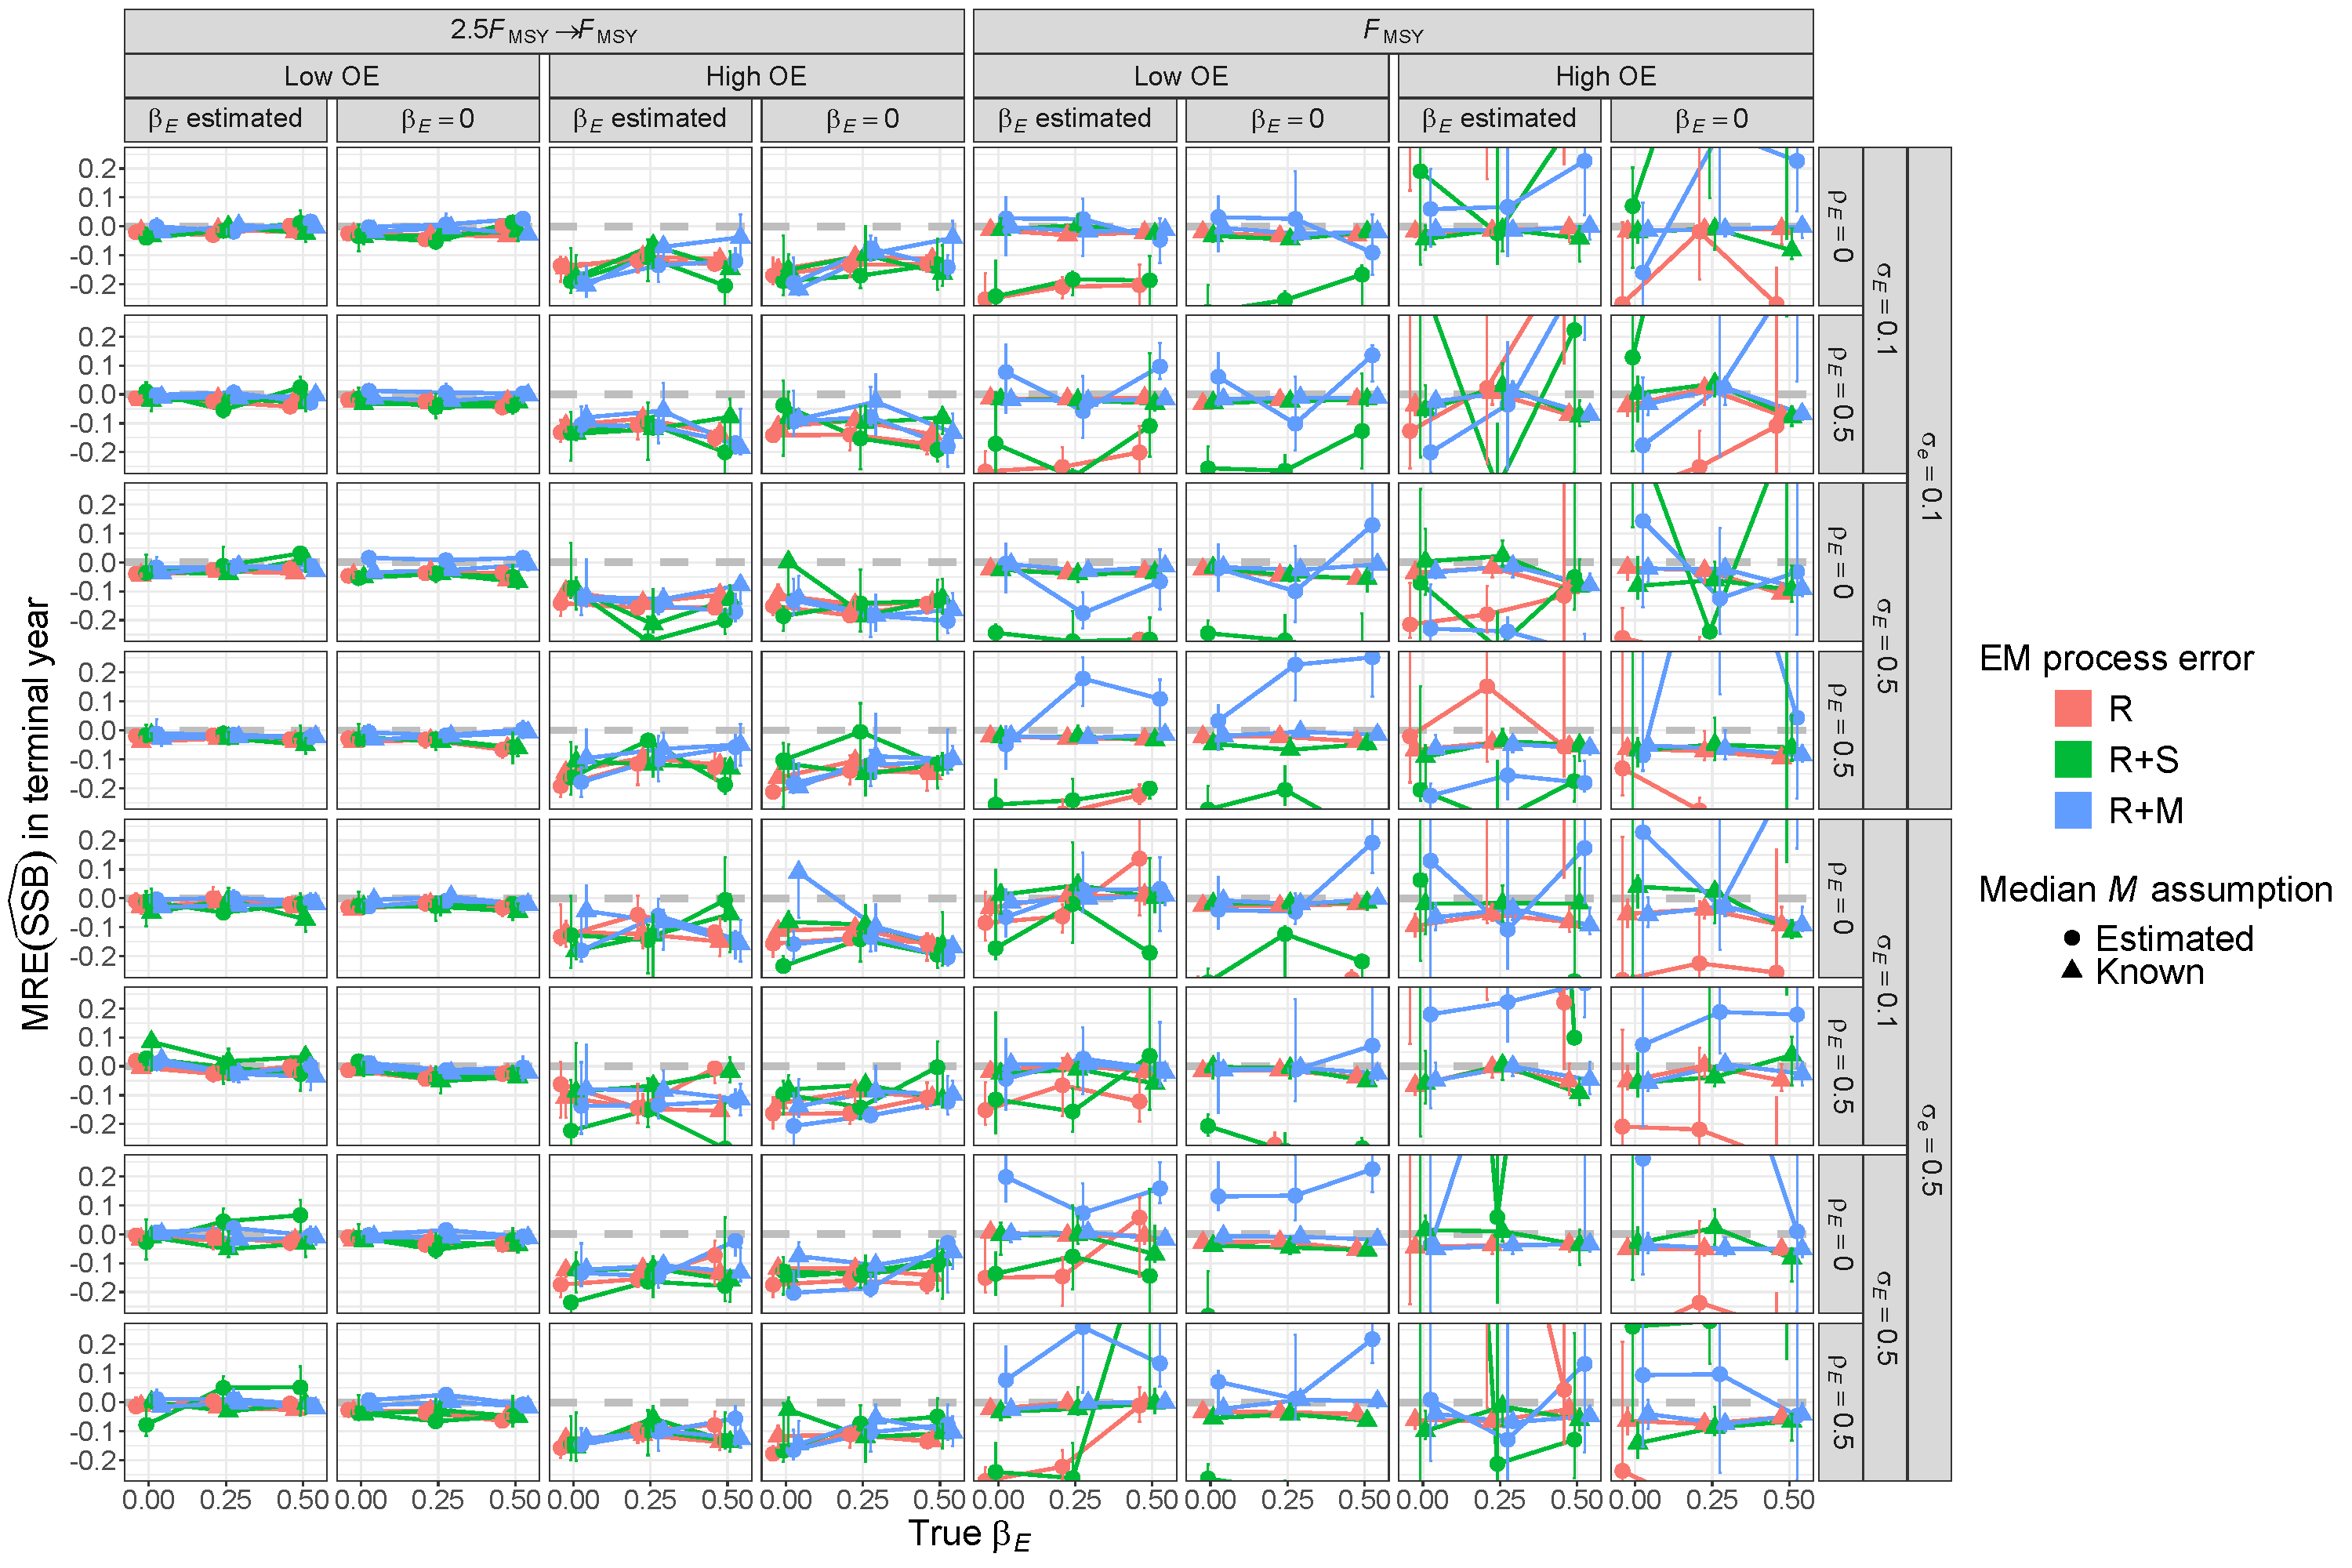
\includegraphics[height = \textheight]{terminal_year_ssb_bias_RMom}
\end{center}
\caption{For R+M operating models, median relative error (MRE) of estimates of SSB in the terminal year for estimating models with alternative process error assumptions, treatment of covariate effect ($\beta_E = 0$ or estimated), and treatment of median $M$ parameter ($\beta_M$ estimated or known).}\label{terminal_ssb_bias_RMom}
\end{figure}
\end{landscape}

\section*{Referenced Tables}\label{referenced-tables}
\addcontentsline{toc}{section}{Referenced Tables}

\begin{table}
\caption{Operating (OM) and estimating model (EM) attributes used in analyses of deviance reduction and classification and regression trees. R, R+S, and R+M, denote models (OM or EM) with process error on recruitment only, recruitment and apparent survival, and recruitment and natural mortality, respectively. SD denotes standard deviation and \Fmsy is the fishing mortality rate that acheives maximum sustainable yield.}\label{factor_table}
{\input{factor_table}}
\end{table}
\pagebreak

\begin{landscape}
\end{landscape}

\section*{Percent deviance reduction
results}\label{percent-deviance-reduction-results}
\addcontentsline{toc}{section}{Percent deviance reduction results}

\subsection*{Estimating model
convergence}\label{estimating-model-convergence}
\addcontentsline{toc}{subsection}{Estimating model convergence}

For fitted logistic regression models to indicators of convergence, the
estimating model process error assumption provided the largest percent
reduction in deviance (9-25\%) of all operating model and estimating
model attributes for all three operating model process error types
(Table \ref{convergence_PRD_table}). Including second order interactions
of operating model and estimating model factors also provided further
reduction of residual deviance (between 7 and 11\%), indicating
successful convergence depended on a combination of operating model and
estimating model attributes.

\subsection*{AIC performance of process error source
selection}\label{aic-performance-of-process-error-source-selection}
\addcontentsline{toc}{subsection}{AIC performance of process error
source selection}

For all OM process error types, the level of error in both the
population and covariate observations were the attributes that resulted
in the largest percent reductions in deviance for multinomial regression
fits to indicators of AIC selection of the process error configuration
(Table \ref{AIC_PE_PRD_table}). For R+S and R+M OMs, level of error in
population observations provided deviance reduction (19\% and 13\%,
respectively) much larger than any other OM and EM factors whereas error
in covariate observations provided the largest reduction (8\%) for R
OMs. Lesser deviance reduction (2-3\%) occurred for the true covariate
effect size and whether the EM made the correct assumption about
including a covariate effect for R OMs and error in covariate
observations for R+M OMs. Including second and third order interactions,
provided the largest reductions in residual deviance for R OMs (24\%)
and little reduction for R+S and R+M OMs (4\% and 6\%, respectively).

\subsection*{AIC performance of covariate effect
selection}\label{aic-performance-of-covariate-effect-selection}
\addcontentsline{toc}{subsection}{AIC performance of covariate effect
selection}

The factors explaining the largest reduction in deviance for logistic
regression models fitted to indicators of AIC selection of the correct
covariate effect assumption depended on the magnitude of the true effect
assumed in the OM (Table \ref{AIC_Ecov_effect_PRD_table}). When OMs had
no covariate effect (\(\beta_E = 0\)) the OM process errror type
provided the largest reduction in deviance (4\%). When OMs assumed a
covariate effect (\(\beta_E>0\)), level of error in population
observations and magnitude of temporal variability in the true covariate
provided the largest reductions in deviance (4\% and 8-21\%,
respectively). The reduction in deviance provided by the magnitude of
covariate temporal variability also increased with larger true covariate
effect. Including second and third order interactions provided a modest
reduction in deviance (5-7\%).

\subsection*{Median natural mortality rate
bias}\label{median-natural-mortality-rate-bias}
\addcontentsline{toc}{subsection}{Median natural mortality rate bias}

Across all OM process error types, regression models fit to errors in
\(\widehat \beta_M\) showed largest reductions in deviance from the type
of OM fishing pressure (4-17\%), EM process error assumption (2-12\%),
and the EM covariate effect assumption (3-7\%, Table
\ref{bias_median_M_converged_PRD_table}). The level of observation error
also provided a similar reduction in deviance for R OMs (3\%).
Relatively large reductions in deviance also occurred with second and
third order interactions (7-16\%).

\subsection*{Median natural mortality rate standard error
bias}\label{median-natural-mortality-rate-standard-error-bias}
\addcontentsline{toc}{subsection}{Median natural mortality rate standard
error bias}

The EM process error assumption provided the largest reduction in
deviance for regression models fitted to errors in
\(\widehat {\text{SE}}\left(\widehat \beta_M\right)\) from R (3\%) and
R+M (7\%) OM simulations (Table \ref{median_M_se_bias_PRD_table}). The
type of OM fishing pressure provided the largest reduction (13\%) for
R+S OMs and a lesser reduction in devaince for R+M OMs (4\%). The EM
covariate effect assumption also provided similar reductions in deviance
for R+S (9\%) and R+M (4\%) OMs.

\subsection*{Median natural mortality rate confidence interval
bias}\label{median-natural-mortality-rate-confidence-interval-bias}
\addcontentsline{toc}{subsection}{Median natural mortality rate
confidence interval bias}

For logistic regressions of indicators of CIs including \(\beta_M\),
factors that provided the largest reductions in deviance were the OM
fishing history and level of error in population observations for all OM
process error types (0.3-6\%) (Table
\ref{mean_M_ci_coverage_PRD_table}). Including second and third order
interactions provided the largest relative increase in deviance
reduction for R+S (8-11\%) and R+M OMs (5-8\%) and lesser increases for
R OMs (3-5\%).

\subsection*{Covariate effect bias}\label{covariate-effect-bias}
\addcontentsline{toc}{subsection}{Covariate effect bias}

For regression models fit to errors in estimation of \(\beta_E\), we
found very little reduction in deviance for any of the OM and EM factors
(Table \ref{bias_ecov_beta_converged_PRD_table}). For the normal model
in these regressions, deviance is the sum of squares and there were
extremely large estimates of \(\beta_E\) (and errors) for many
simulations which resulted in extremely large sums of squares and
relative differences from the null model were therefore small
(\textless1\%). Nevertheless, observation error of the covariate
provided either the largest or second largest reductions in deviance of
any of the single OM and EM attributes for OM process error
configuration types. OM fishing history provided reductions of similar
scale for R and R+S OMs. Other factors providing similar reductions were
true covariate effect size for R OMs and level of error in population
observations and EM process error assumption for R+S OMs. Including
second and third order interactions also provided further reductions in
residual deviance similar in scale to the individual factors.

\subsection*{Covariate effect standard error
bias}\label{covariate-effect-standard-error-bias}
\addcontentsline{toc}{subsection}{Covariate effect standard error bias}

Factors providing the largest reductions in deviance for estimation
error of \(\widehat {\text{SE}}\left(\widehat\beta_E\right)\) were
generally similar to those that were most important for estimation of
\(\beta_E\), but deviance reductions were one or two orders of magnitude
larger (Table \ref{bias_ecov_beta_se_PRD_table}). Level of error in
covariate observations and EM process error assumption was important for
all OM process error configurations (6-13\% and 3-4\%, respectively).
Level of error in population observations provided relatively large
reductions in deviance for R+S and R+M OMs (3\% and 8\%, respectively).
The OM fishing pressure history provided a lesser reduction in deviance
for all OM process error types (2-4\%). Like estimation of \(\beta_E\),
additional large reductions in deviance also occurred when second and
third order interactions of OM and EM attributes were included in the
regression models (11-31\%).

\subsection*{Covariate effect confidence interval
bias}\label{covariate-effect-confidence-interval-bias}
\addcontentsline{toc}{subsection}{Covariate effect confidence interval
bias}

For logistic regressions of indicators of CIs including the true value
of \(\beta_E\), factors that provided the largest reductions in deviance
were true covariate effect size for R and R+M OMs (11\% and 3\%,
respectively) and EM process error configuration for R+S OMs (7\%)
(Table \ref{ecov_beta_ci_coverage_PRD_table}). Covariate observation
error also provided relatively large reduction in deviance for R OMs
(8\%). Lesser reductions of 1-2\% occurred for level of error in
population observations and covariate temporal variability for all OM
process error types. Including second and third order interactions also
provided relatively large further reductions in deviance (5-9\%).

\subsection*{Terminal year natural morality rate
bias}\label{terminal-year-natural-morality-rate-bias}
\addcontentsline{toc}{subsection}{Terminal year natural morality rate
bias}

Regressions of estimation errors show largest reductions in deviance
from whether the EM treats \(\beta_M\) as known (Table
\ref{bias_M_PRD_table}). For R and R+S OMs, annual \(M\) was constant,
and therefore, terminal \(M\) was known when the true \(\beta_M\) was
assumed known and there will be no error in any of those EMs. Beyond the
\(\beta_M\) assumption, the OM fishing history, level of error in
population observations, and EM assumptions for covariate effect and
process error all provided notable deviance reductions.

\subsection*{Terminal year natural morality rate
accuracy}\label{terminal-year-natural-morality-rate-accuracy}
\addcontentsline{toc}{subsection}{Terminal year natural morality rate
accuracy}

Like bias of terminal year \(M\), the EM assumption for \(\beta_M\)
provided the largest reduction in deviance (22-45\%) for accuracy as
measured by RMSE for all OM process error types (Table
\ref{rmse_M_PRD_table}). Including second and third order interactions
also provided large further reductions in deviance (21-38\%).

Using correlation to measure accuracy of terminal year \(M\) estimation
provides a different perspective. Treatment of \(\beta_M\) provided
relatively large reductions in deviance for all OM process error types
(3-12\%), but level of variability in the covariate was equally or more
important (3-15\%) as was whether the covariate effect was included in
the EM (12\%) for R and R+S OMs (Table \ref{corr_M_PRD_table}).
Including second and third order interactions also provided relatively
large ruther reductions in deviance (15 to 24\%).

\subsection*{Terminal year spawning stock biomass
bias}\label{terminal-year-spawning-stock-biomass-bias}
\addcontentsline{toc}{subsection}{Terminal year spawning stock biomass
bias}

Regression model fits showed largest reductions in deviance for OM
fishing history (2-3\%), error in population observations (1\% for R and
R+M OMs), and EM \(\beta_M\) assumption (2\%; Table
\ref{bias_SSB_PRD_table}). The type of EM process error assumed also
provided a deviance reduction similar in scale for R+S OMs (1\%).
Including second and third order interactions of OM and EM attributes
provided further deviance reductions of 5-10\%.

\subsection*{Terminal year spawning stock biomass
accuracy}\label{terminal-year-spawning-stock-biomass-accuracy}
\addcontentsline{toc}{subsection}{Terminal year spawning stock biomass
accuracy}

Largest reductions in deviance were provided by whether \(\beta_M\) was
known or estimated (20-21\%) and whether there was temporal contrast in
fishing pressure (20-33\%) across all OM process error types (Table
\ref{rmse_SSB_PRD_table}). Lesser reductions were also provided by the
EM process error assumption for R and R+M OMs. Inclusion of second and
third order interactions of OM and EM attributes provided further
reductions in deviance of 26-40\%.

Using correlation to measure accuracy, temporal contrast in fishing
pressure and EM treatment of \(\beta_M\) provided relatively important
reductions in deviance like RMSE, but level of error in population
observations was important rather than EM process error type (Table
\ref{corr_ssb_PRD_table}). Including second and third order interactions
also provided relatively large ruther reductions in deviance (6 to
20\%).

\begin{table}
\caption{Percent reduction in deviance for logistic regression models fit to indicators of convergence (providing Hessian-based standard errors). Table rows give each operating model (OM) and estimating model (EM) factor included individually, combined, and with second and third order interactions. Table columns categorize operating models (OMs) with process error on recruitment only (R), recruitment and apparent survival (R+S), or recruitment and natural mortality (R+M). See Table \ref{factor_table} for further details.}\label{convergence_PRD_table}
{\input{convergence_PRD_table}}
\end{table}
\pagebreak

\begin{table}
\caption{Percent reduction in deviance for multinomial logistic regression models fit to indicators of process error assumption in the estimating models with lowest AIC. See Tables \ref{convergence_PRD_table} and \ref{factor_table} for further details.}\label{AIC_PE_PRD_table}
{\input{AIC_PE_PRD_table}}
\end{table}
\pagebreak

\begin{table}
\caption{Percent reduction in deviance for logistic regression models fit to indicators of correct estimating model (EM) covariate effect assumption (no effect for operating models assuming $\beta_E = 0$ or estimated effect for operating models assuming $\beta_E > 0$) with lowest AIC. Table columns categorize operating models with different true values for $\beta_E$. See Tables \ref{convergence_PRD_table} and \ref{factor_table} for further details.}\label{AIC_Ecov_effect_PRD_table}
{\input{AIC_Ecov_effect_PRD_table}}
\end{table}
\pagebreak

\begin{table}
\caption{Percent reduction in deviance for linear regression models fit to errors in estimation of the median natural mortality rate parameter ($\widehat \beta_M$). See Tables \ref{convergence_PRD_table} and \ref{factor_table} for further details.}\label{bias_median_M_converged_PRD_table}
{\input{mean_M_bias_converged_PRD_table}}
\end{table}
\pagebreak

\begin{table}
\caption{Percent reduction in deviance for linear regression models fit to errors in estimation of the Hessian-based standard error of the median $M$ parameter ($\widehat {\text{SE}}\left(\widehat \beta_M\right)$). See Tables \ref{convergence_PRD_table} and \ref{factor_table} for further details.}\label{median_M_se_bias_PRD_table}
{\input{mean_M_se_PRD_table}}
\end{table}
\pagebreak

\begin{table}
\caption{Percent reduction in deviance for logistic regression models fit to indicators of whether CIs for estimates of the median natural mortality rate parameter ($\widehat \beta_M$) includes the true value. See Tables \ref{convergence_PRD_table} and \ref{factor_table} for further details.}\label{mean_M_ci_coverage_PRD_table}
{\input{mean_M_ci_coverage_PRD_table}}
\end{table}
\pagebreak

\begin{table}
\caption{Percent reduction in deviance for linear regression models fit to errors in estimation of the covariate effect on natural mortality rate ($\widehat \beta_E$). See Tables \ref{convergence_PRD_table} and \ref{factor_table} for further details.}\label{bias_ecov_beta_converged_PRD_table}
{\input{ecov_beta_bias_converged_PRD_table}}
\end{table}
\pagebreak

\begin{table}
\caption{Percent reduction in deviance for linear regression models fit to errors in estimation of the Hessian-based standard error of the covariate effect on $M$ ($\widehat {\text{SE}}\left(\widehat \beta_E\right)$). See Tables \ref{convergence_PRD_table} and \ref{factor_table} for further details.}\label{bias_ecov_beta_se_PRD_table}
{\input{ecov_beta_se_PRD_table}}
\end{table}
\pagebreak

\begin{table}
\caption{Percent reduction in deviance for logistic regression models fit to indicators of whether CIs for covariate effect estimates includes the true value. See Tables \ref{convergence_PRD_table} and \ref{factor_table} for further details.}\label{ecov_beta_ci_coverage_PRD_table}
{\input{ecov_beta_ci_coverage_PRD_table}}
\end{table}
\pagebreak

\begin{table}
\caption{Percent reduction in deviance for linear regression models fit to errors in terminal year natural mortality rate ($M$) as measured by Eq. 2. See Tables \ref{convergence_PRD_table} and \ref{factor_table} for further details.}\label{bias_M_PRD_table}
{\input{bias_M_PRD_table}}
\end{table}
\pagebreak

\begin{table}
\caption{Percent reduction in deviance for linear regression models fit to log-transformed RMSE of terminal year natural mortality ($M$). See Tables \ref{convergence_PRD_table} and \ref{factor_table} for further details.}\label{rmse_M_PRD_table}
{\input{rmse_M_PRD_table}}
\end{table}
\pagebreak

\begin{table}
\caption{Percent reduction in deviance for linear regression models fit to correlation of terminal year natural mortality ($M$) estimates and true values. See Tables \ref{convergence_PRD_table} and \ref{factor_table} for further details.}\label{corr_M_PRD_table}
{\begin{center}
\begin{tabular}{lrrr}
\hline\hline
\multicolumn{1}{l}{Factor}&\multicolumn{1}{c}{R}&\multicolumn{1}{c}{R+S}&\multicolumn{1}{c}{R+M}\tabularnewline
\hline
OM $F$ history& 0.05& 0.02& 0.37\tabularnewline
OM Obs. Error& 2.00& 0.89& 3.73\tabularnewline
$OM \sigma_e$& 2.30& 2.56& 0.37\tabularnewline
$OM \sigma_E$&14.91&13.78& 3.03\tabularnewline
$OM \rho_{E}$& 1.98& 0.33& 0.14\tabularnewline
OM $\beta_{E}$& 0.41& 3.76& 3.87\tabularnewline
EM Process Error& 0.43& 1.52& 0.62\tabularnewline
$EM \beta_{E}$ assumption&12.72&12.30& 1.56\tabularnewline
EM $M$ assumption&12.34& 7.16& 3.03\tabularnewline
All factors&42.11&38.31&15.76\tabularnewline
+ All Two Way&63.38&62.40&31.99\tabularnewline
+ All Three Way&72.79&75.98&46.62\tabularnewline
\hline
\end{tabular}\end{center}
}
\end{table}
\pagebreak

\begin{table}
\caption{Percent reduction in deviance for linear regression models fit to errors in terminal year spawning stock biomass (SSB) as measured by Eq. 2. See Tables \ref{convergence_PRD_table} and \ref{factor_table} for further details.}\label{bias_SSB_PRD_table}
{\input{bias_SSB_PRD_table}}
\end{table}
\pagebreak

\begin{table}
\caption{Percent reduction in deviance for linear regression models fit to log-transformed RMSE of terminal year spawning stock biomass (SSB). See Tables \ref{convergence_PRD_table} and \ref{factor_table} for further details.}\label{rmse_SSB_PRD_table}
{\input{rmse_ssb_PRD_table}}
\end{table}
\pagebreak

\begin{table}
\caption{Percent reduction in deviance for linear regression models fit to correlation of terminal year spawning stock biomass (SSB) estimates and true values. See Tables \ref{convergence_PRD_table} and \ref{factor_table} for further details.}\label{corr_ssb_PRD_table}
{\input{corr_ssb_PRD_table}}
\end{table}
\pagebreak

\section*{Further detailed results}\label{further-detailed-results}
\addcontentsline{toc}{section}{Further detailed results}

\begin{landscape}
\begin{figure}
\begin{center}
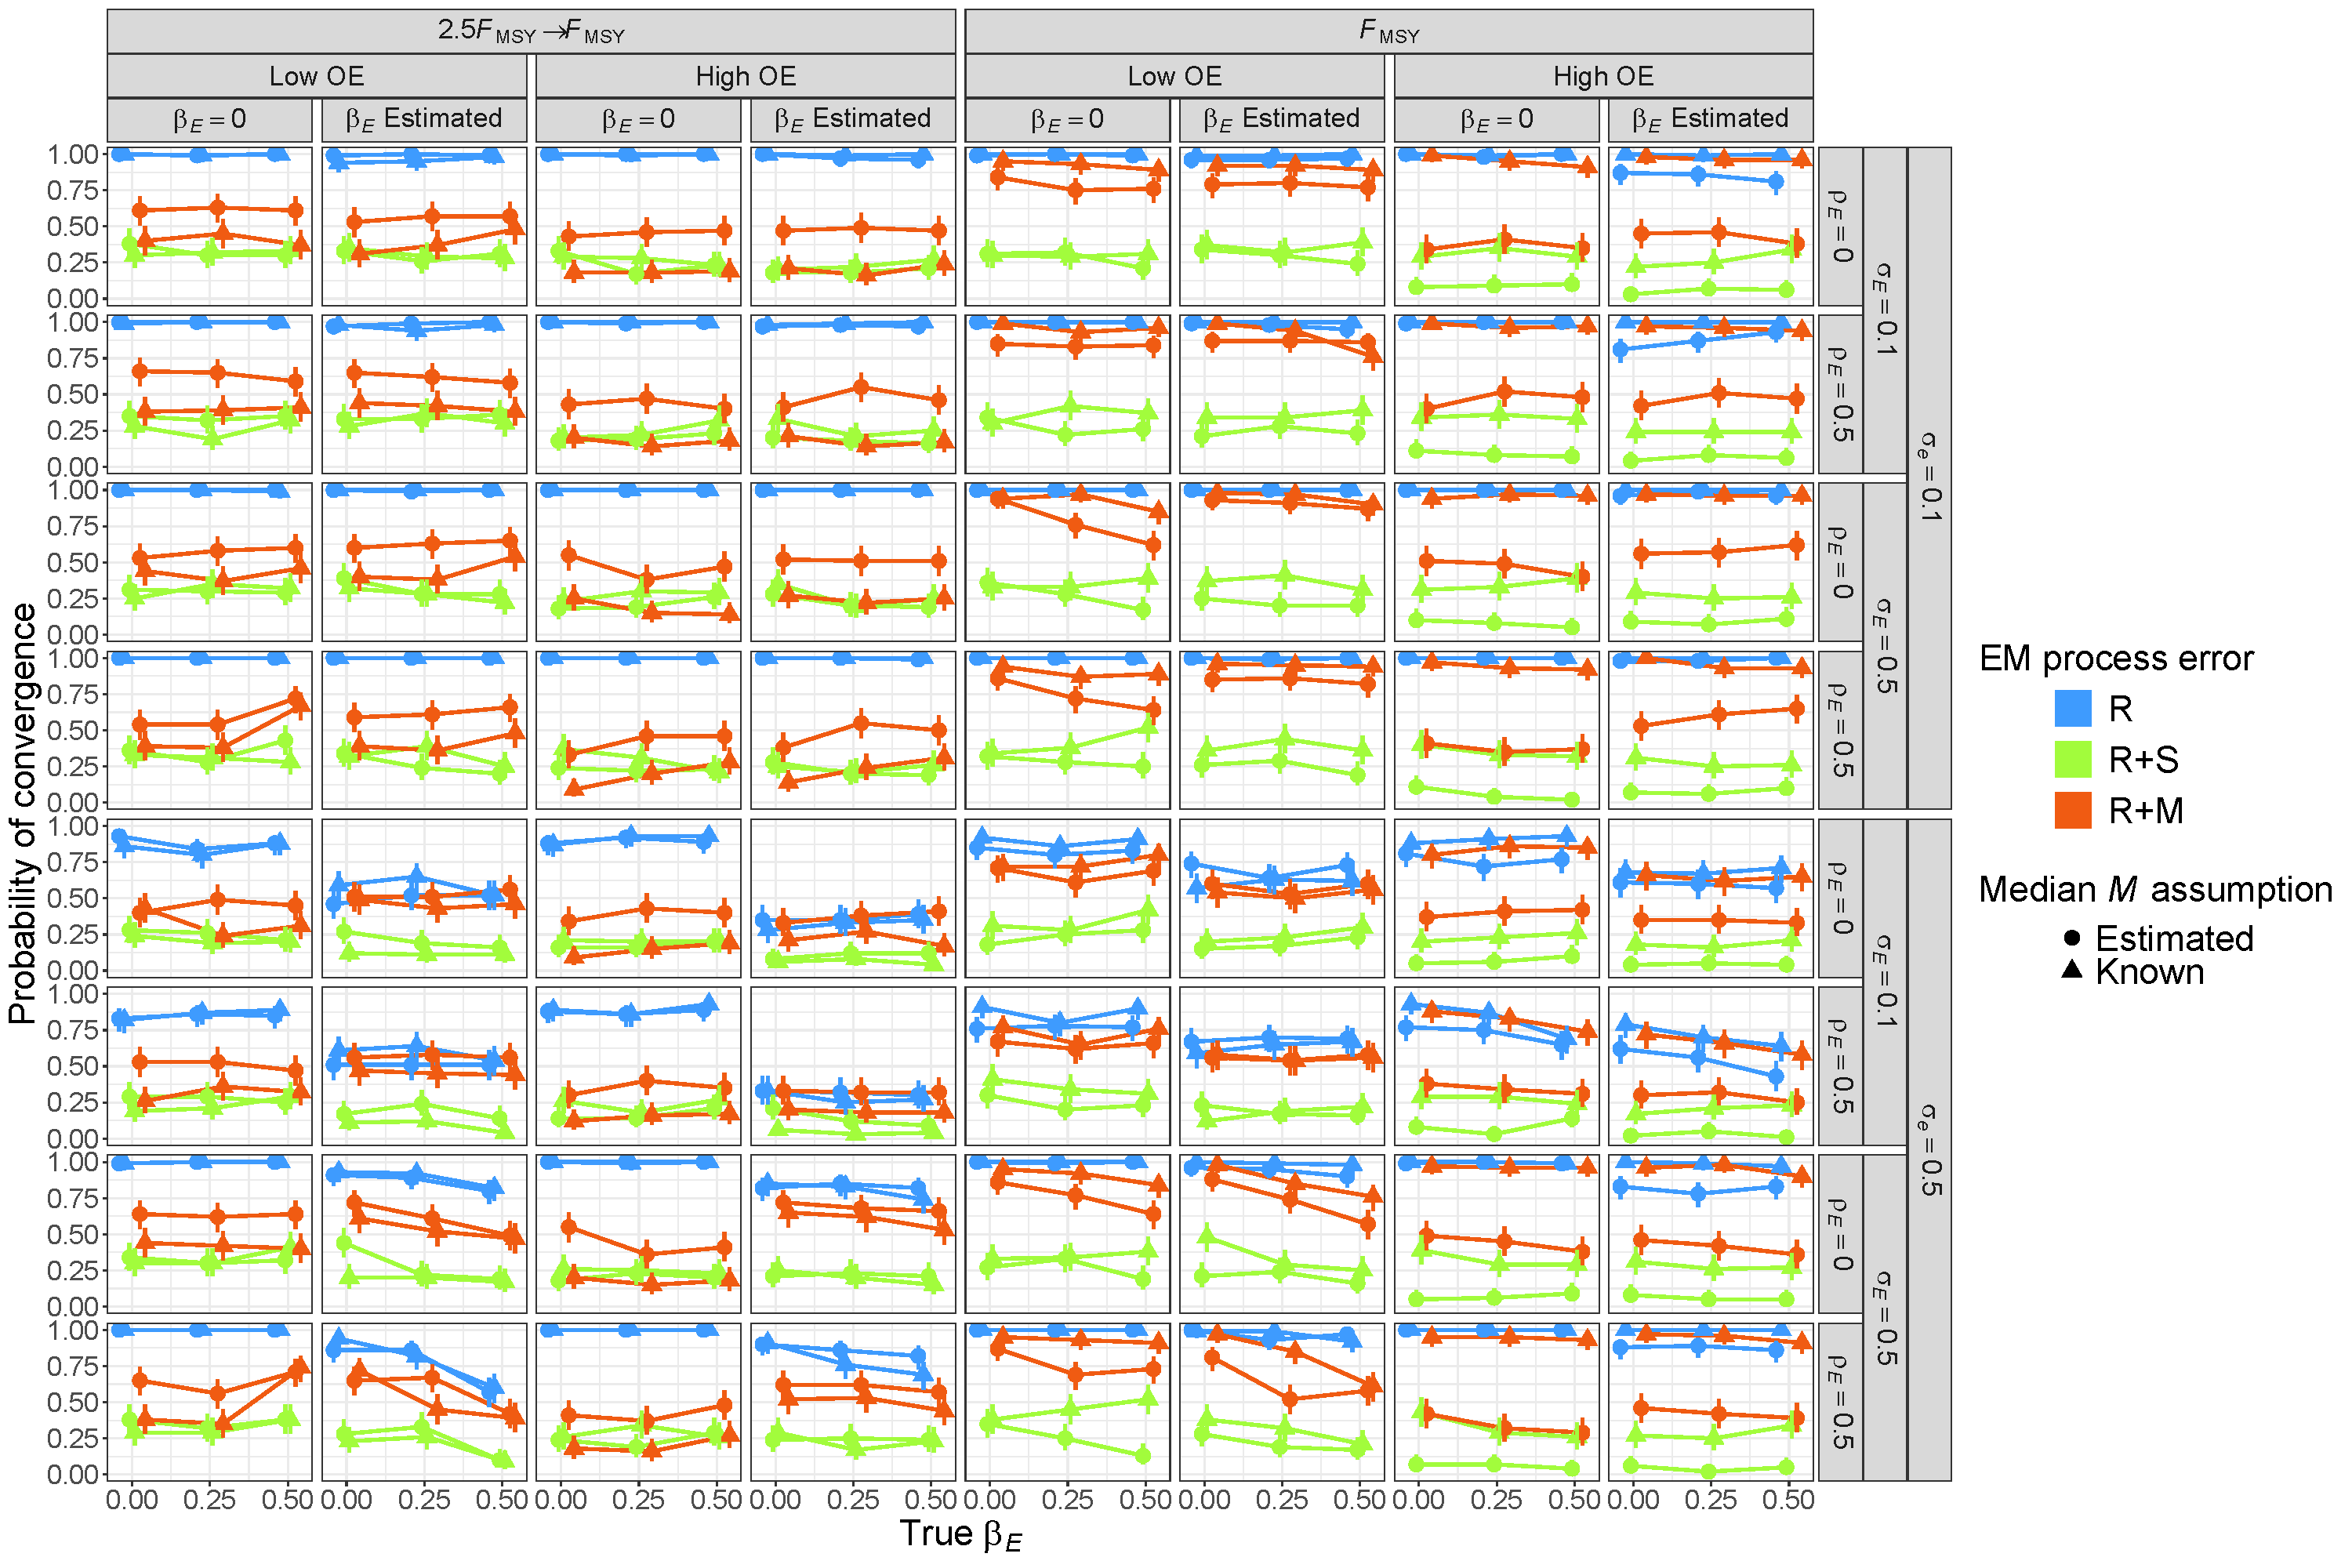
\includegraphics[height = \textheight]{convergence_Rom}
\end{center}
\caption{Estimated probability of fits providing Hessian-based standard errors for estimating models assuming alternative process error, that estimate or assume known median $M$, and that estimate or assume no covariate effect on median $M$ when fitted to R operating models and three levels of true covariate effect on median $M$ (x axis). Vertical lines represent 95\% confidence intervals.}\label{convergence_Rom}
\end{figure}
\end{landscape}

\begin{landscape}
\begin{figure}
\begin{center}
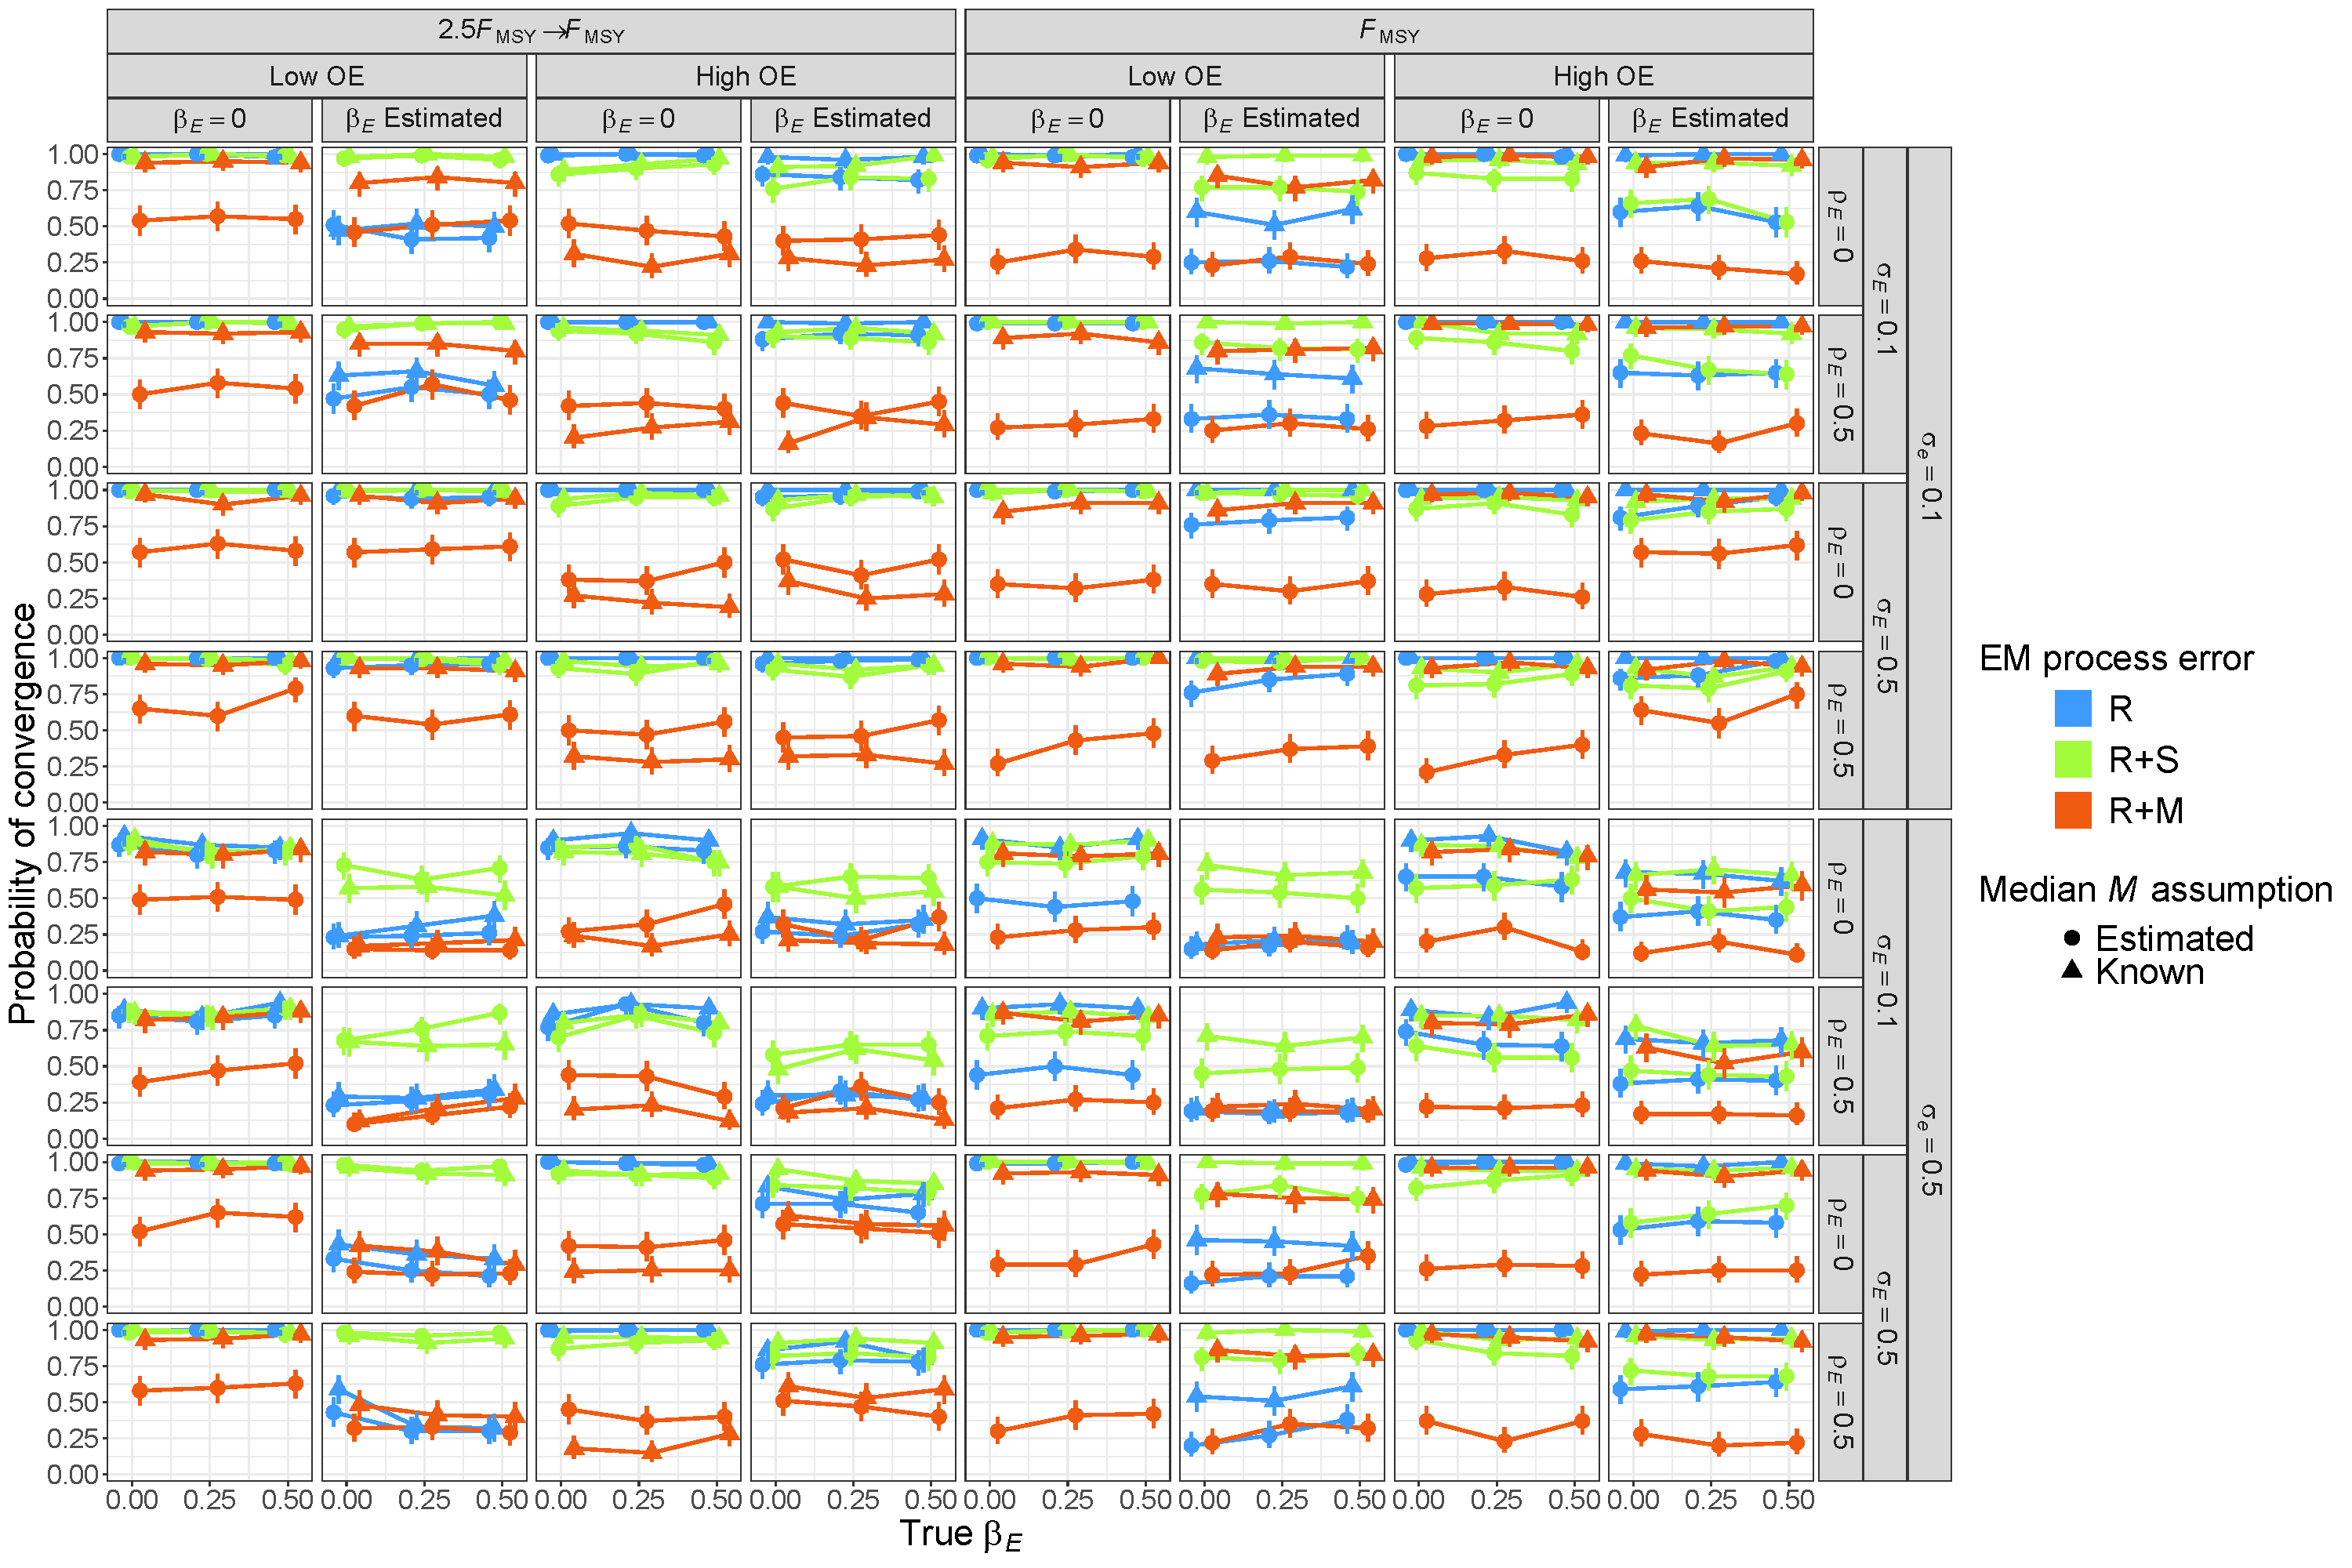
\includegraphics[height = \textheight]{convergence_RSom}
\end{center}
\caption{Estimated probability of fits providing Hessian-based standard errors for estimating models assuming alternative process error, that estimate or assume known median $M$, and that estimate or assume no covariate effect on median $M$ when fitted to R+S operating models and three levels of true covariate effect on median $M$ (x axis). Vertical lines represent 95\% confidence intervals.}\label{convergence_RSom}
\end{figure}
\end{landscape}

\begin{landscape}
\begin{figure}
\begin{center}
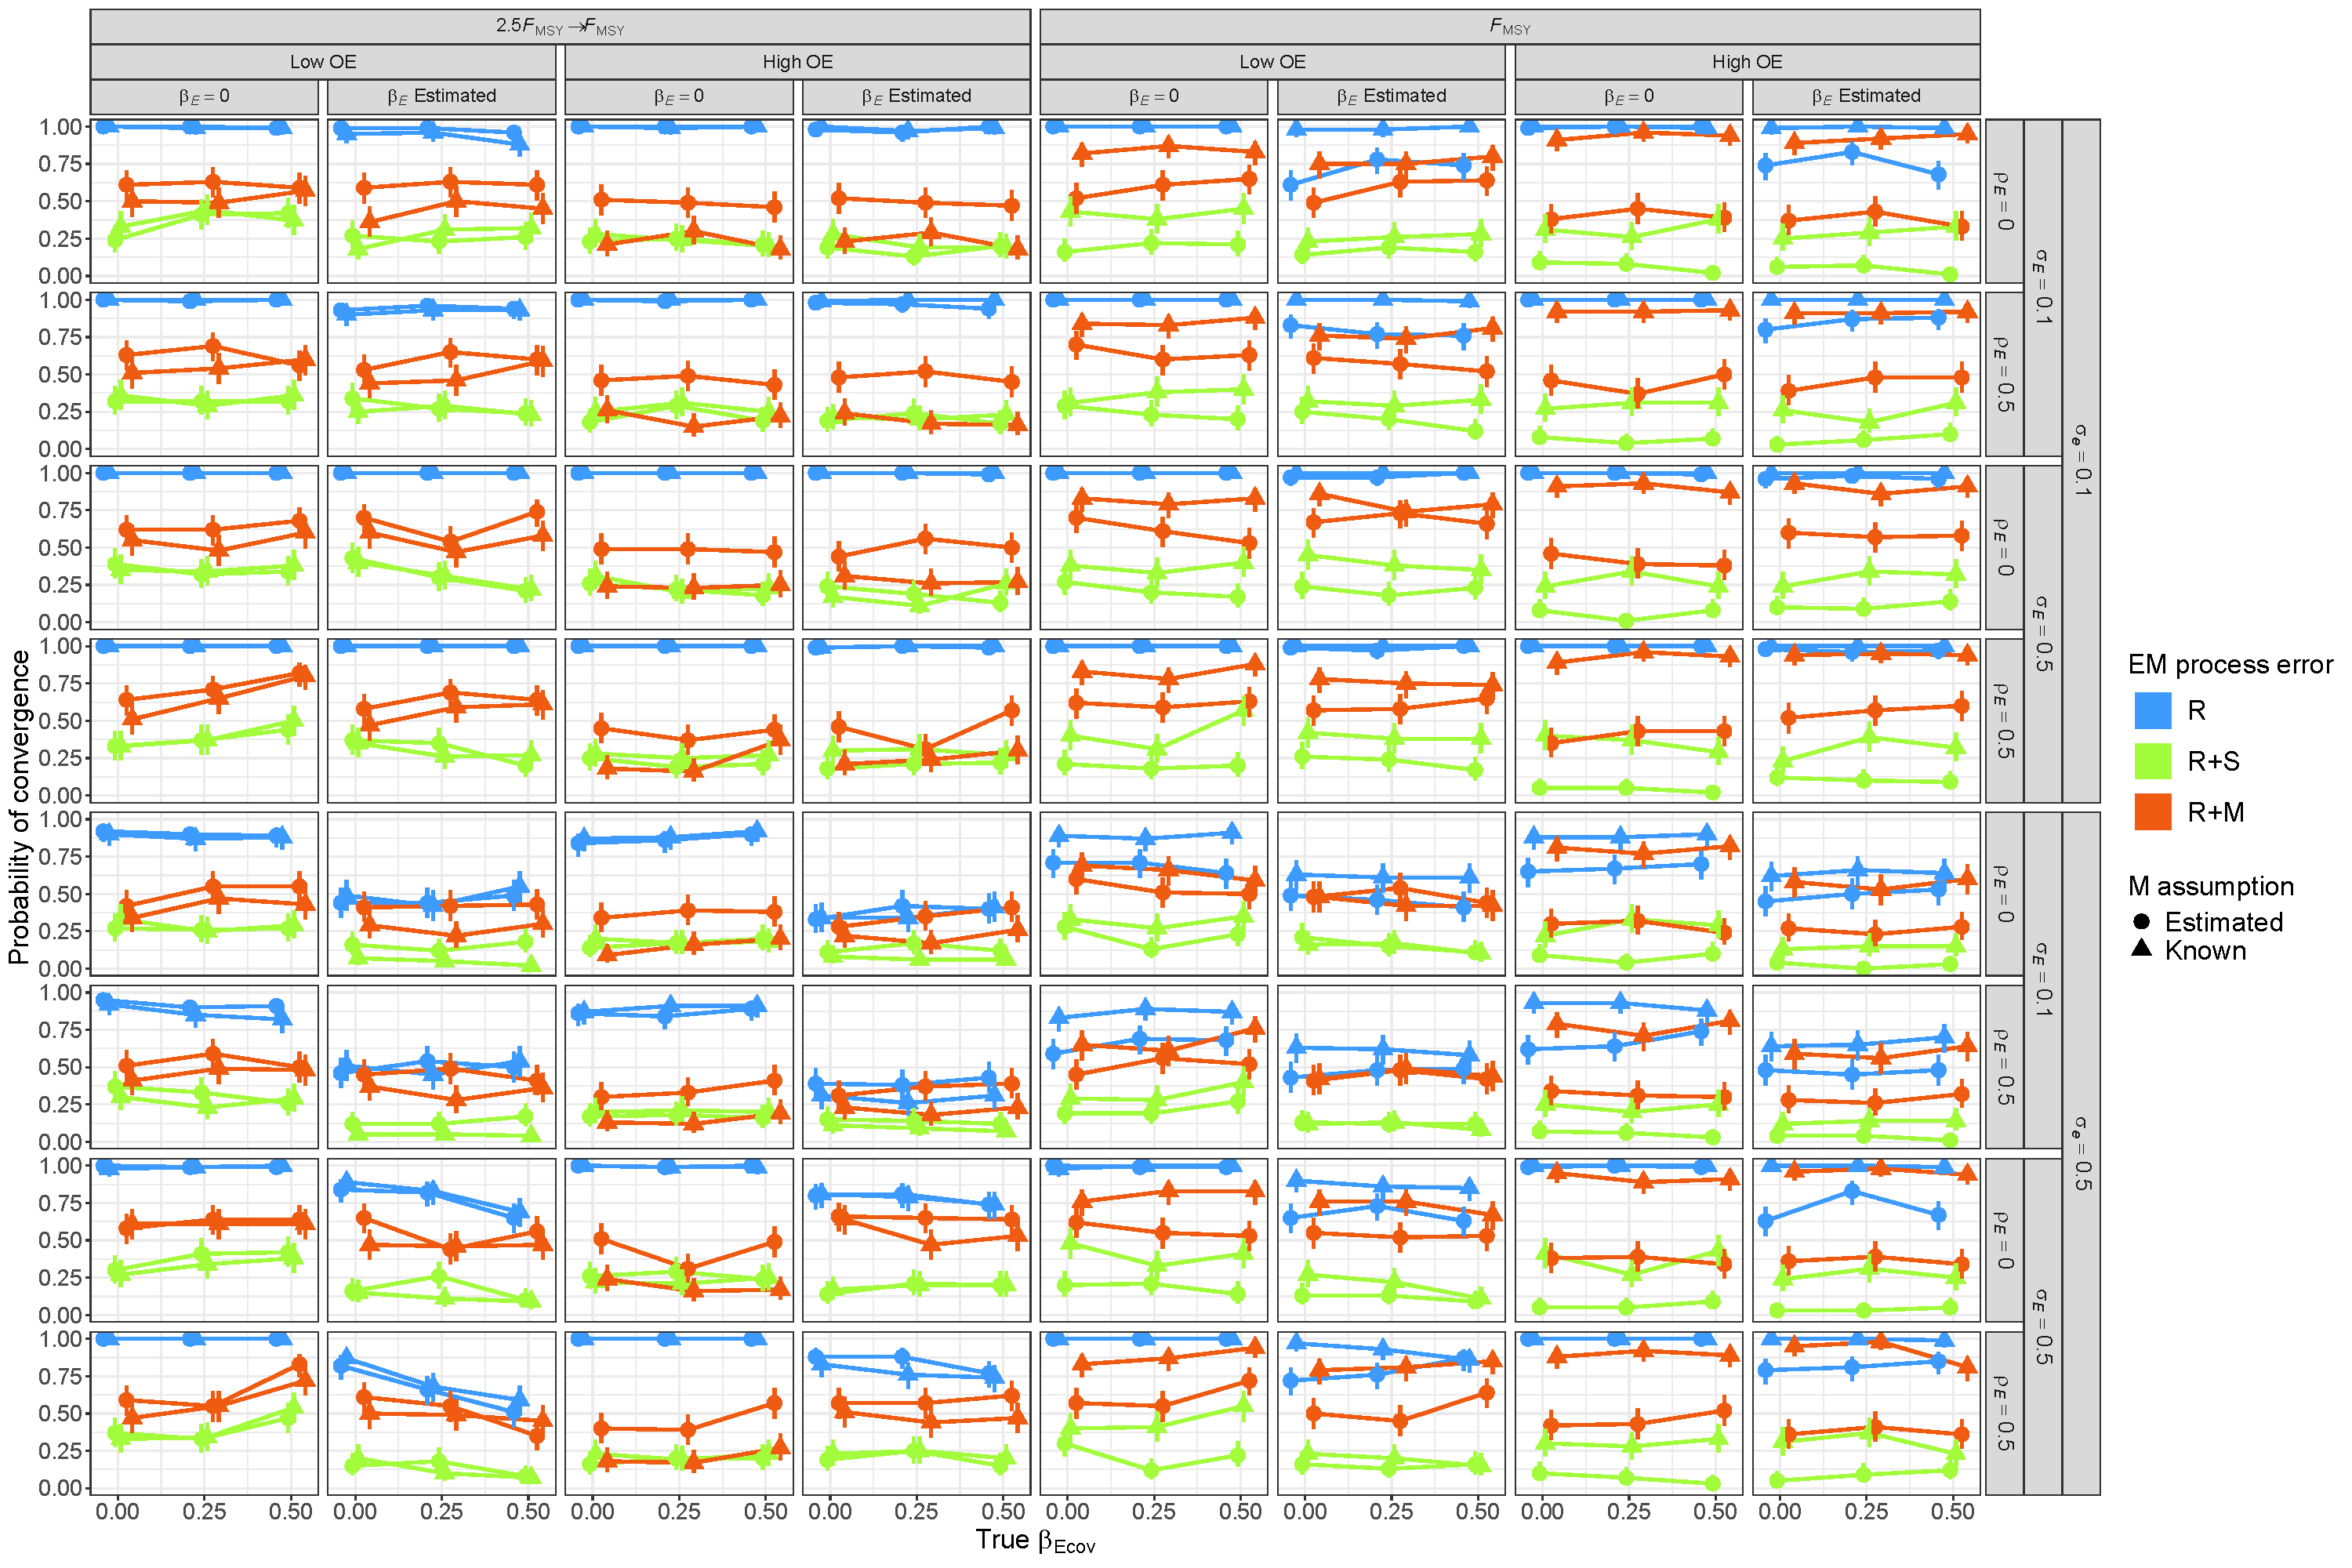
\includegraphics[height = \textheight]{convergence_RMom}
\end{center}
\caption{Estimated probability of fits providing Hessian-based standard errors for estimating models assuming alternative process error, that estimate or assume known median $M$, and that estimate or assume no covariate effect on median $M$ when fitted to R+M operating models and three levels of true covariate effect on median $M$ (x axis). Vertical lines represent 95\% confidence intervals.}\label{convergence_RMom}
\end{figure}
\end{landscape}

\begin{landscape}
\begin{figure}
\begin{center}
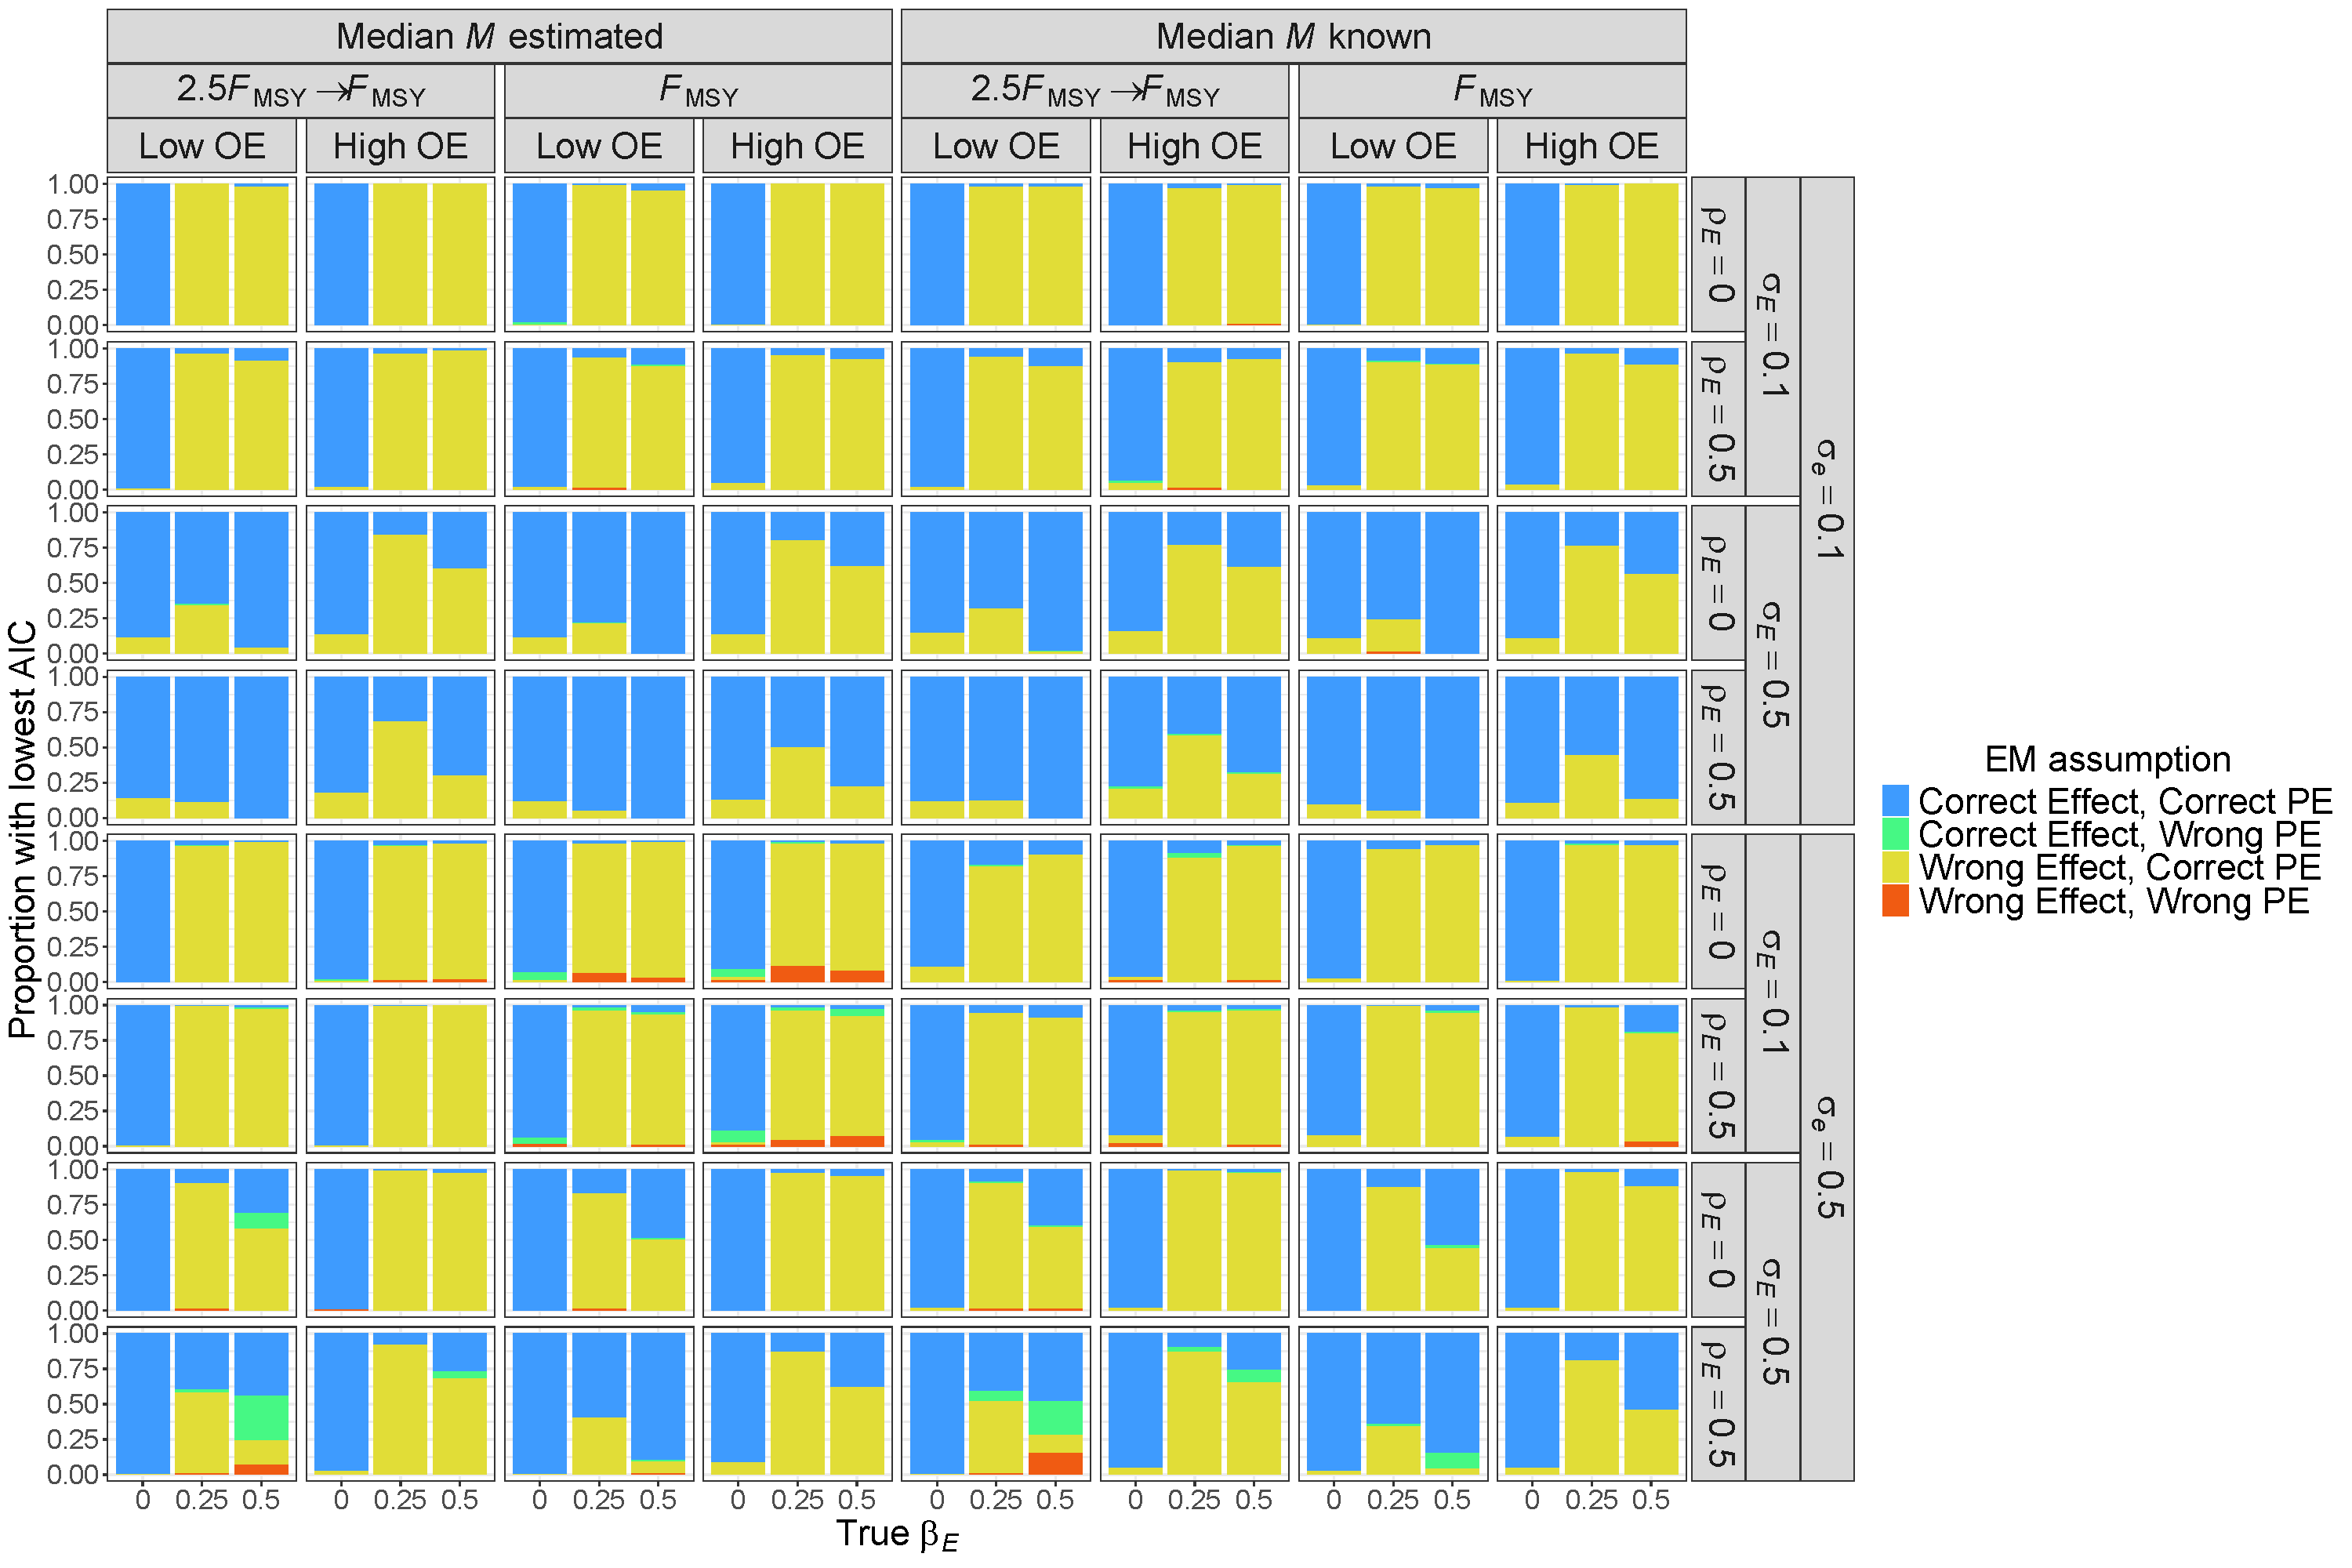
\includegraphics[height = \textheight]{aic_Rom}
\end{center}
\caption{Proportion of simulated data sets for R operating models where the estimating model type (treatment of environmental covariate and assumed process error type) had the lowest AIC.}\label{aic_Rom}
\end{figure}
\end{landscape}

\begin{landscape}
\begin{figure}
\begin{center}
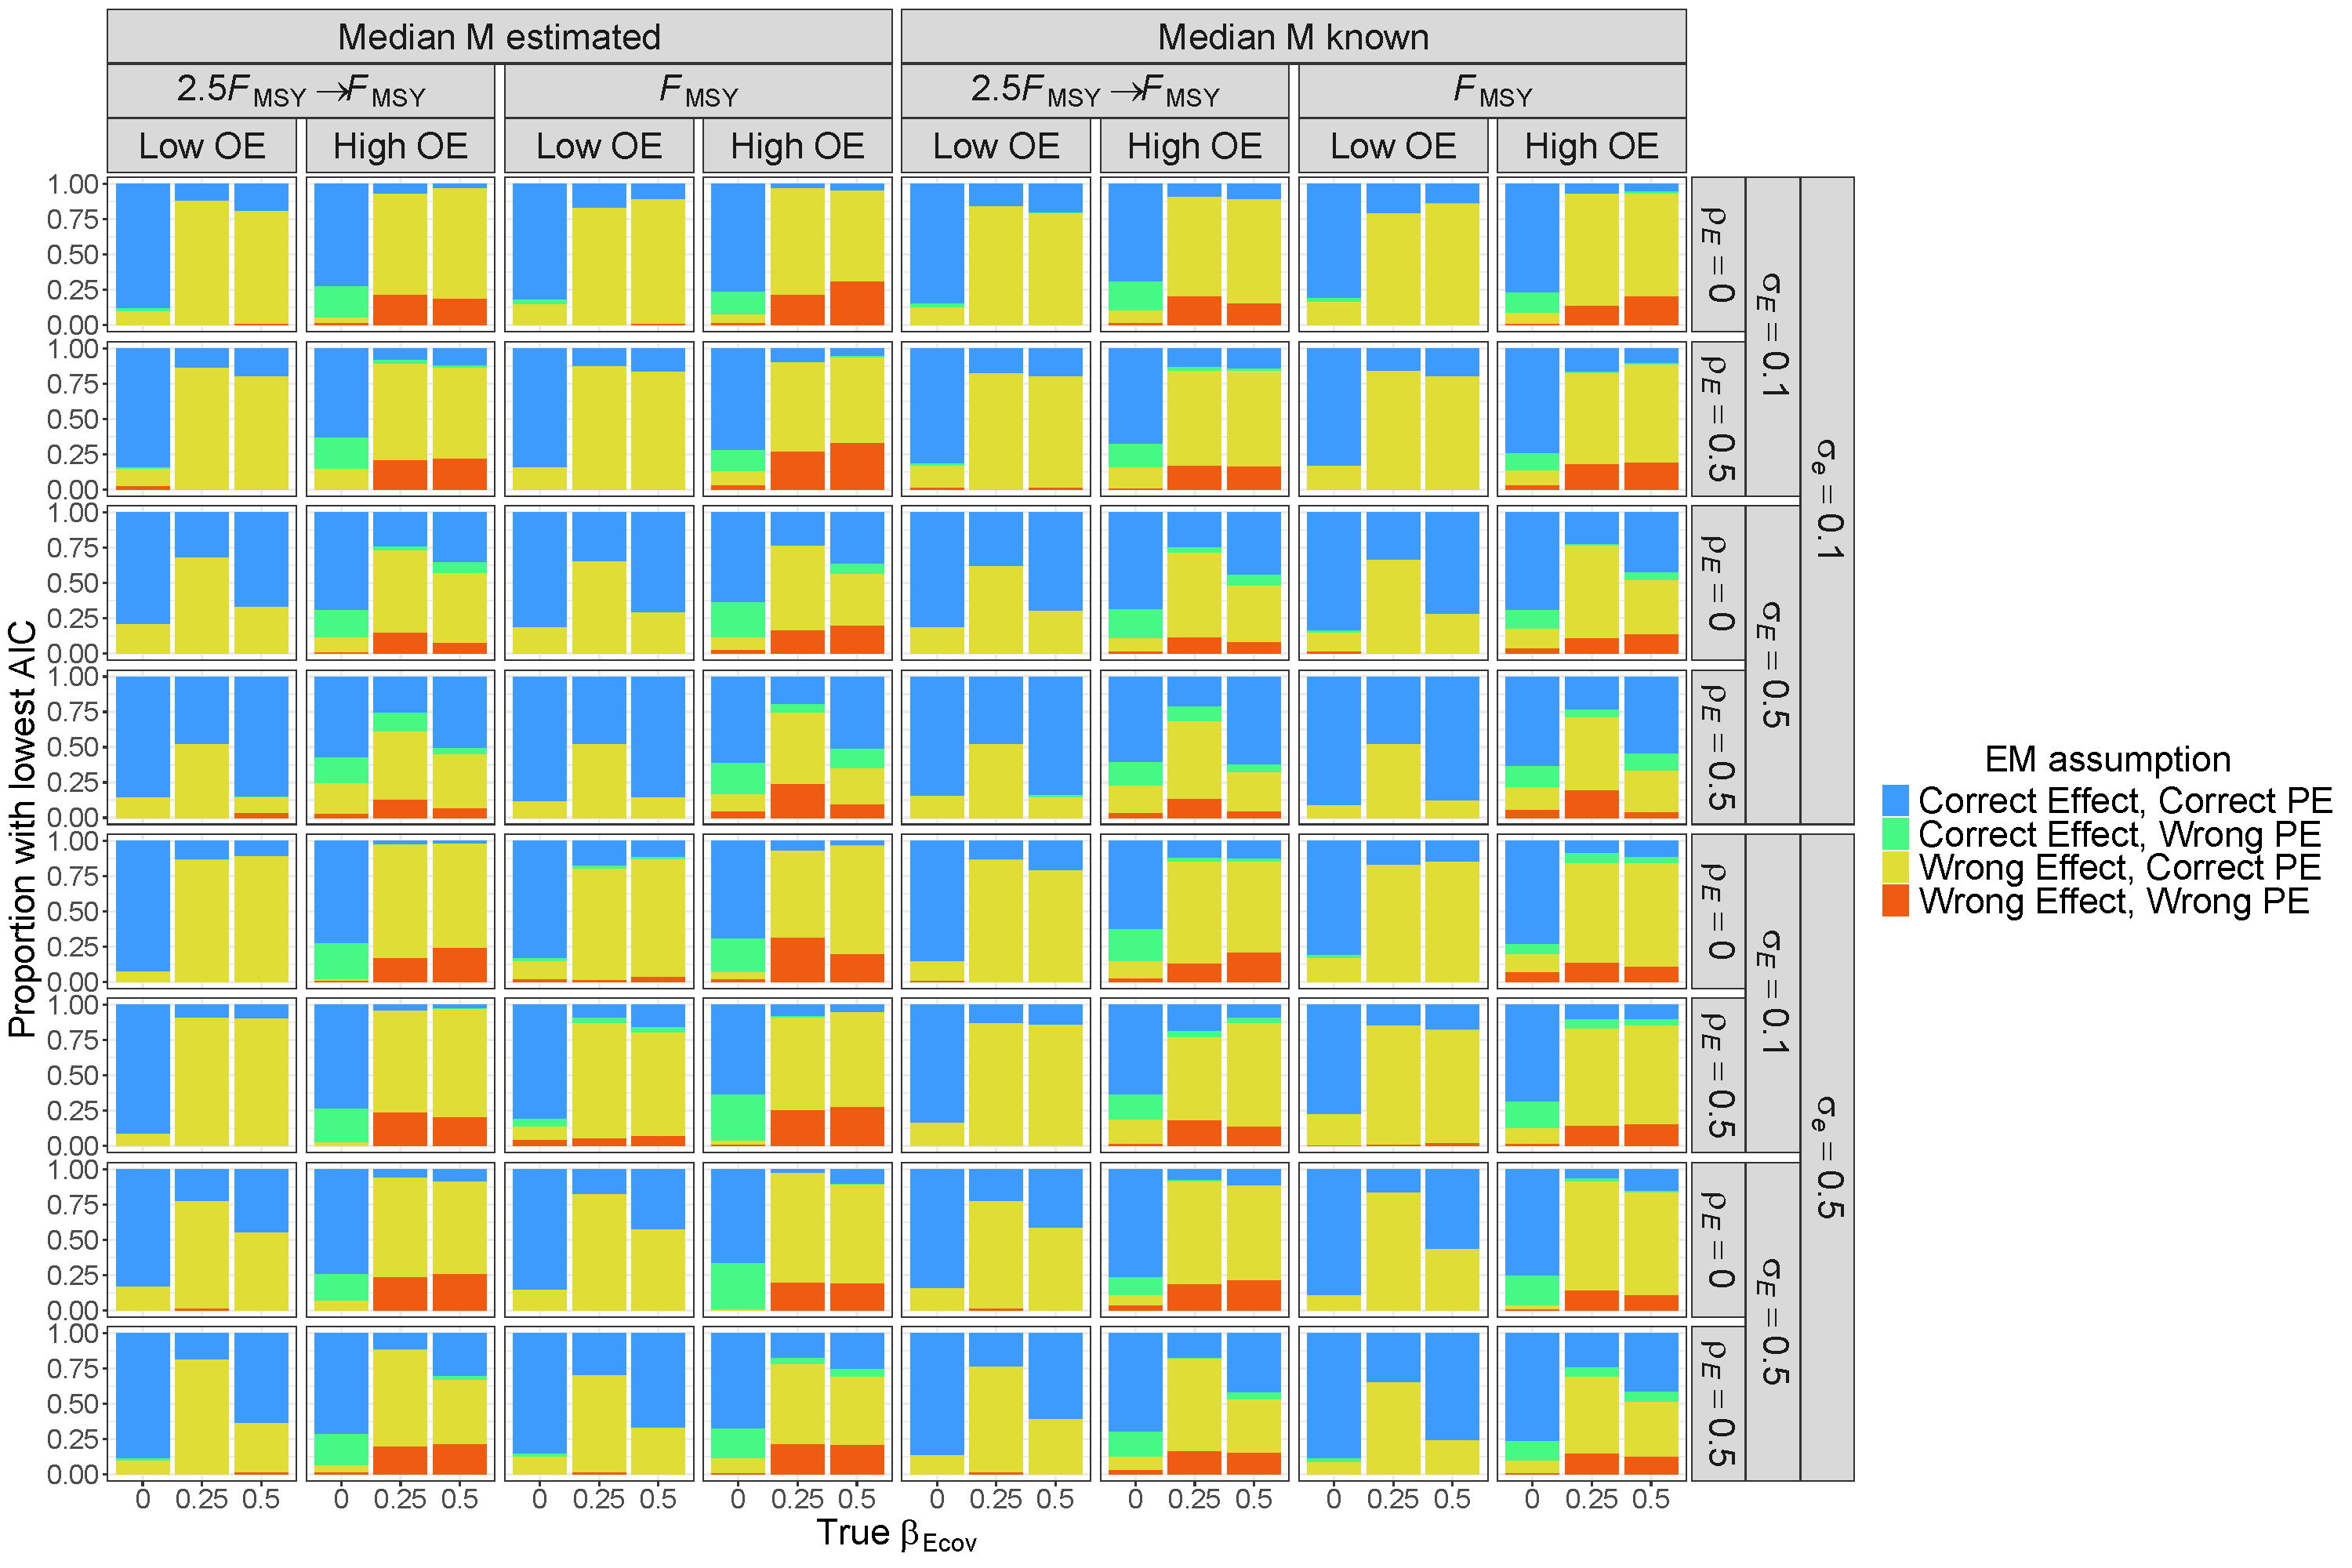
\includegraphics[height = \textheight]{aic_RSom}
\end{center}
\caption{Proportion of simulated data sets for R+S operating models where the estimating model type (treatment of environmental covariate and assumed process error type) had the lowest AIC.}\label{aic_RSom}
\end{figure}
\end{landscape}

\begin{landscape}
\begin{figure}
\begin{center}
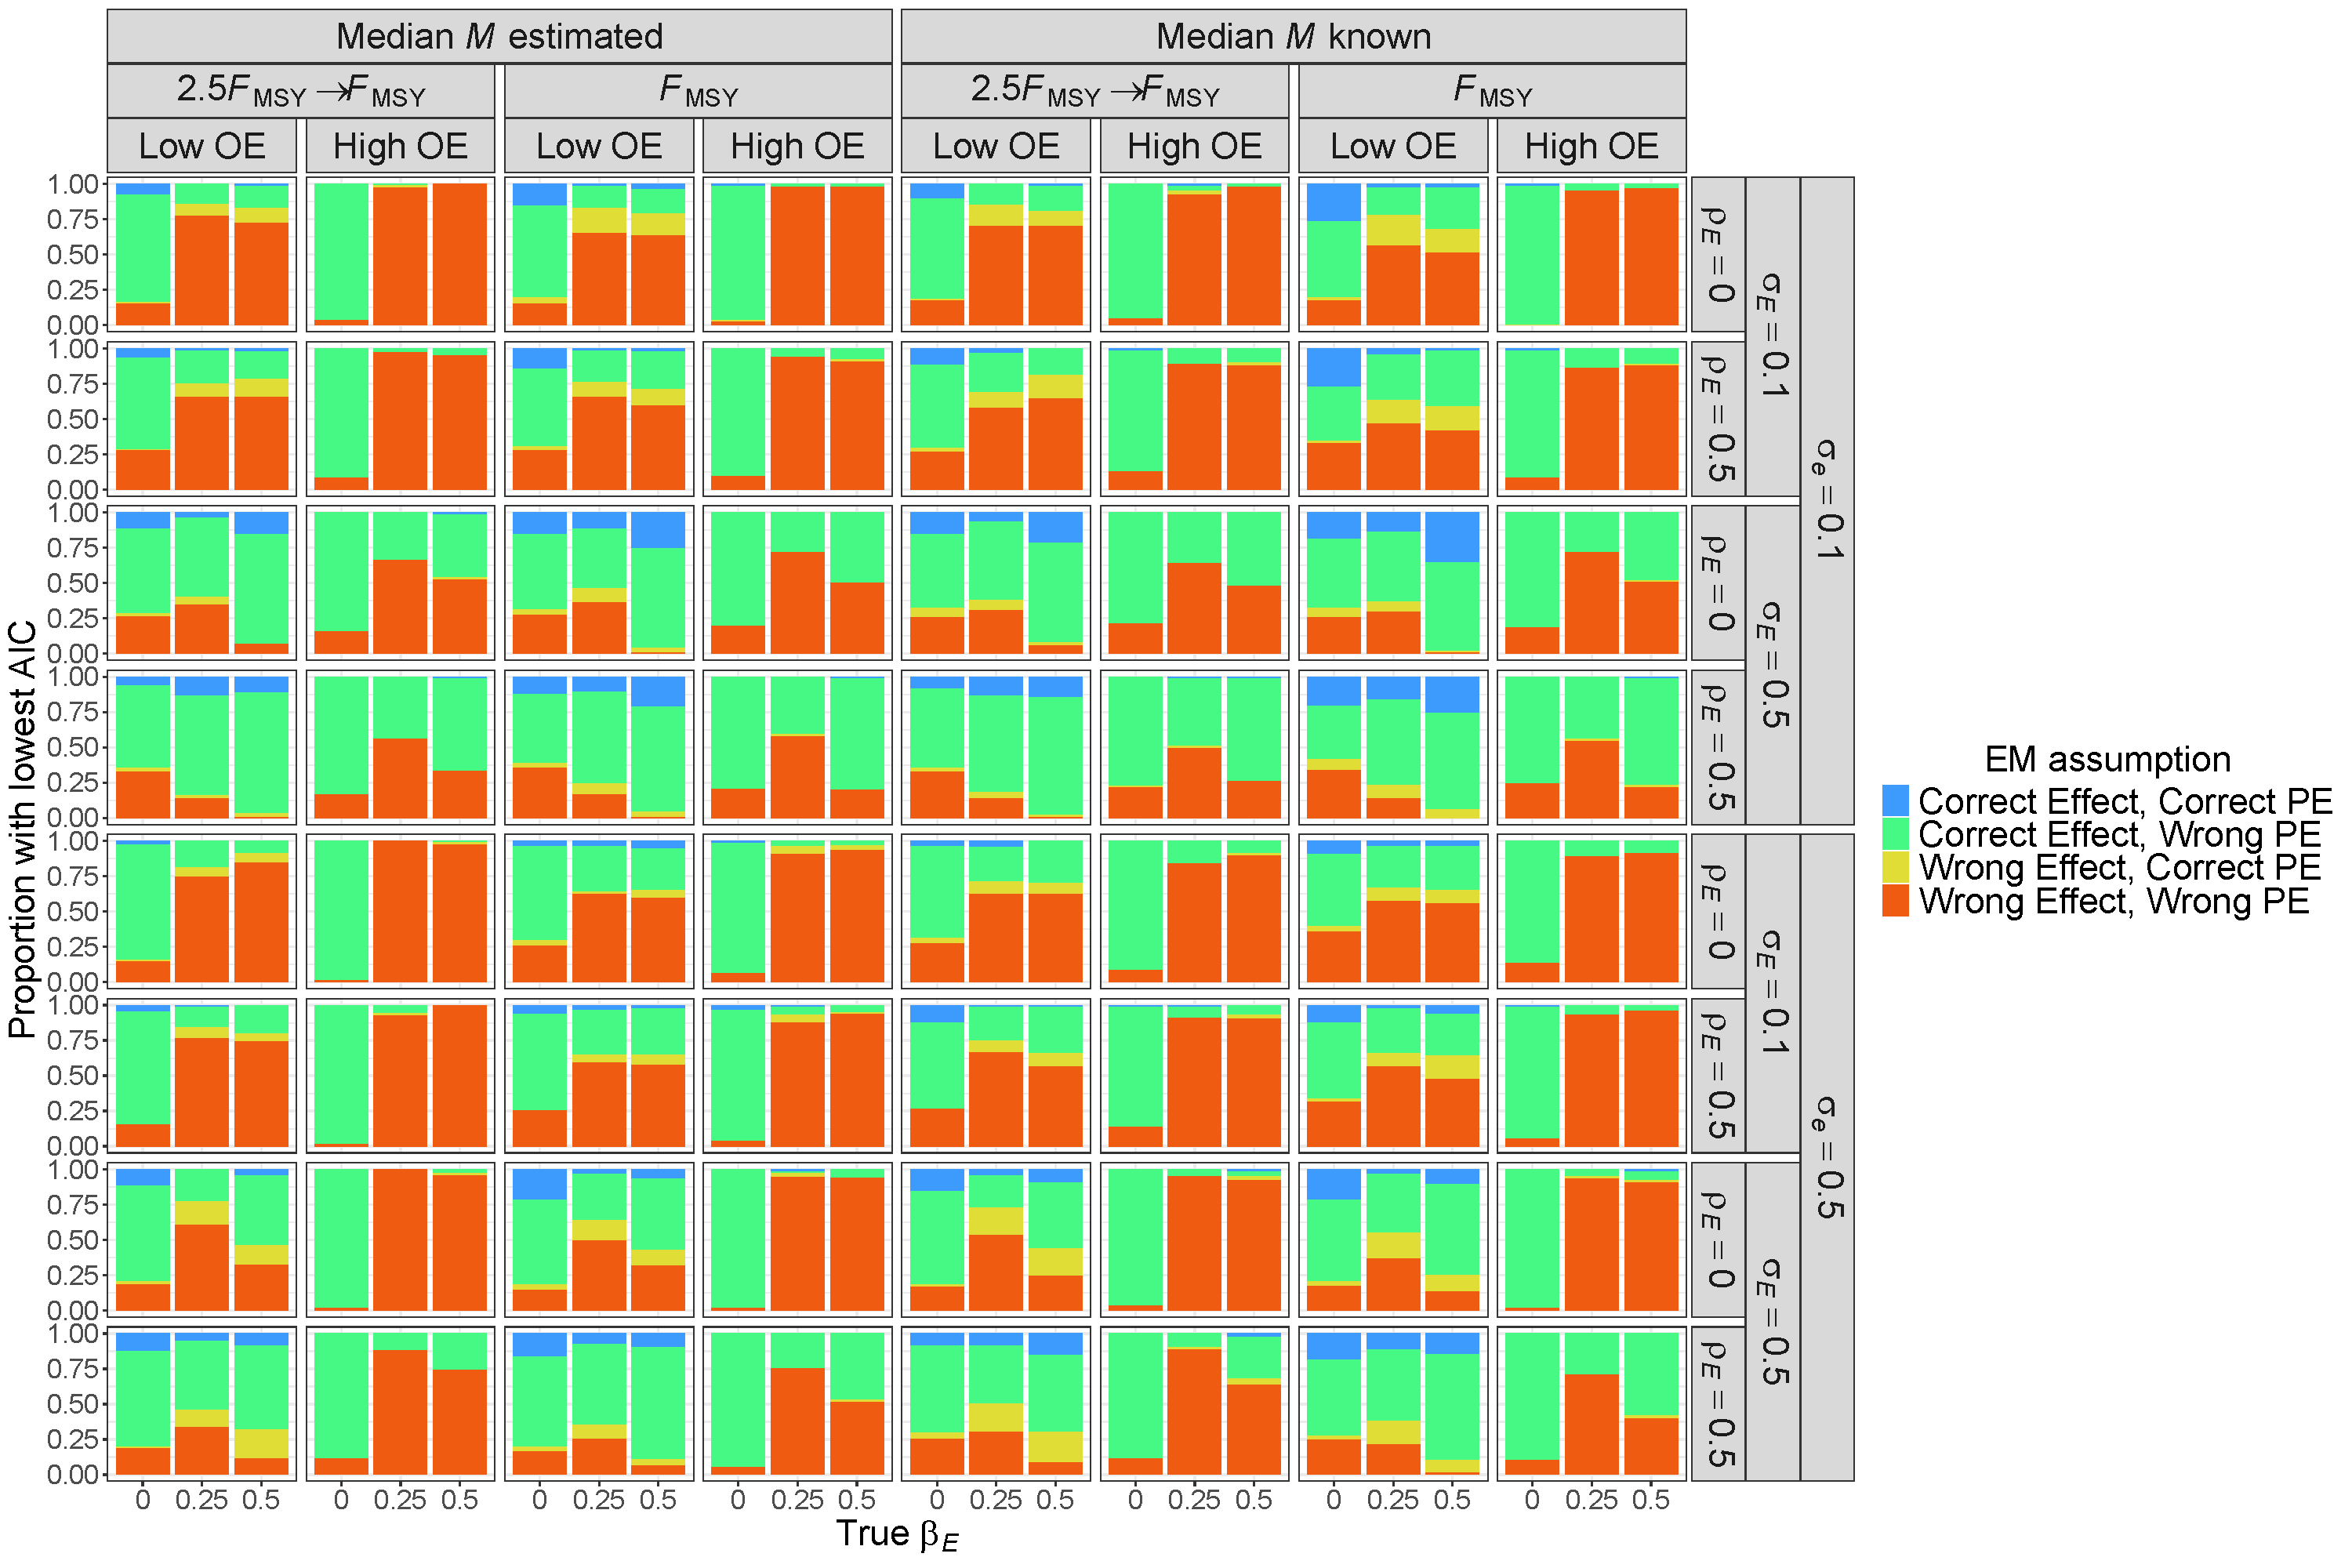
\includegraphics[height = \textheight]{aic_RMom}
\end{center}
\caption{Proportion of simulated data sets for R+M operating models where the estimating model type (treatment of environmental covariate and assumed process error type) had the lowest AIC.}\label{aic_RMom}
\end{figure}
\end{landscape}

\begin{landscape}
\begin{figure}
\begin{center}
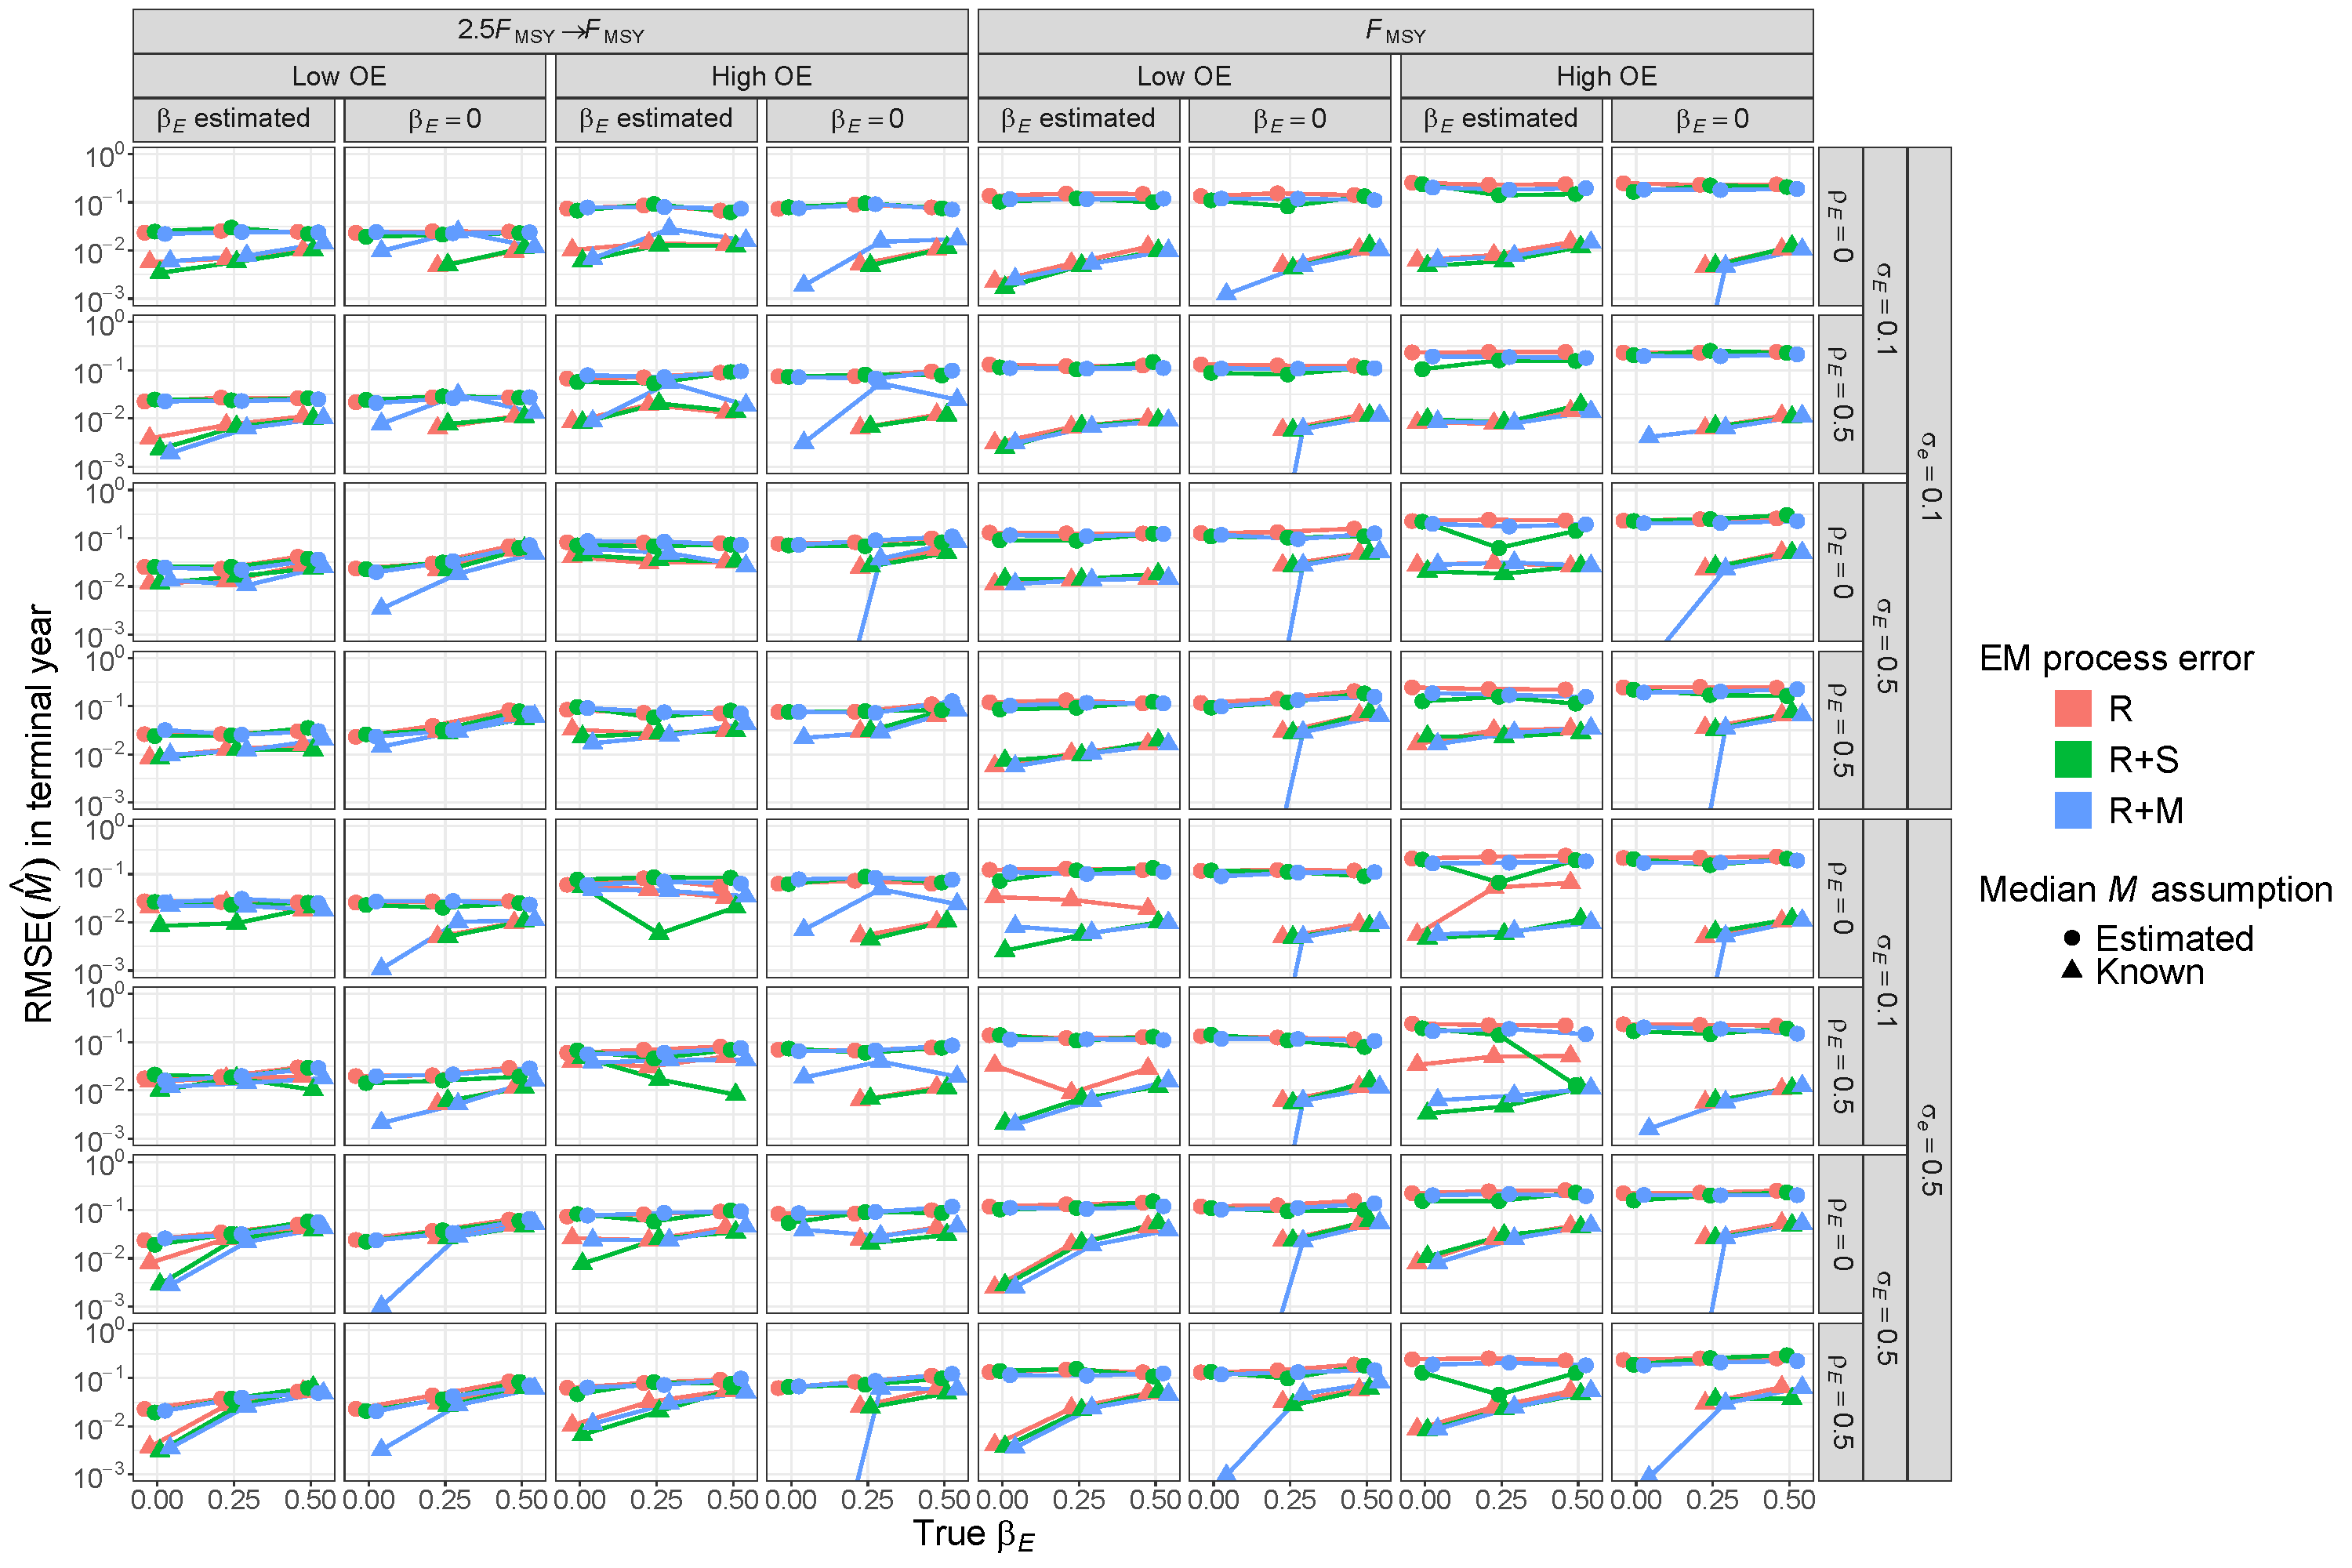
\includegraphics[height = \textheight]{terminal_year_M_rmse_Rom}
\end{center}
\caption{For R operating models, RMSE of estimates of terminal year $M$ for estimating models with alternative process error assumptions, treatment of covariate effect ($\beta_E = 0$ or estimated), and treatment of median $M$ parameter ($\beta_M$ estimated or known).}\label{terminal_M_rmse_Rom}
\end{figure}
\end{landscape}

\begin{landscape}
\begin{figure}
\begin{center}
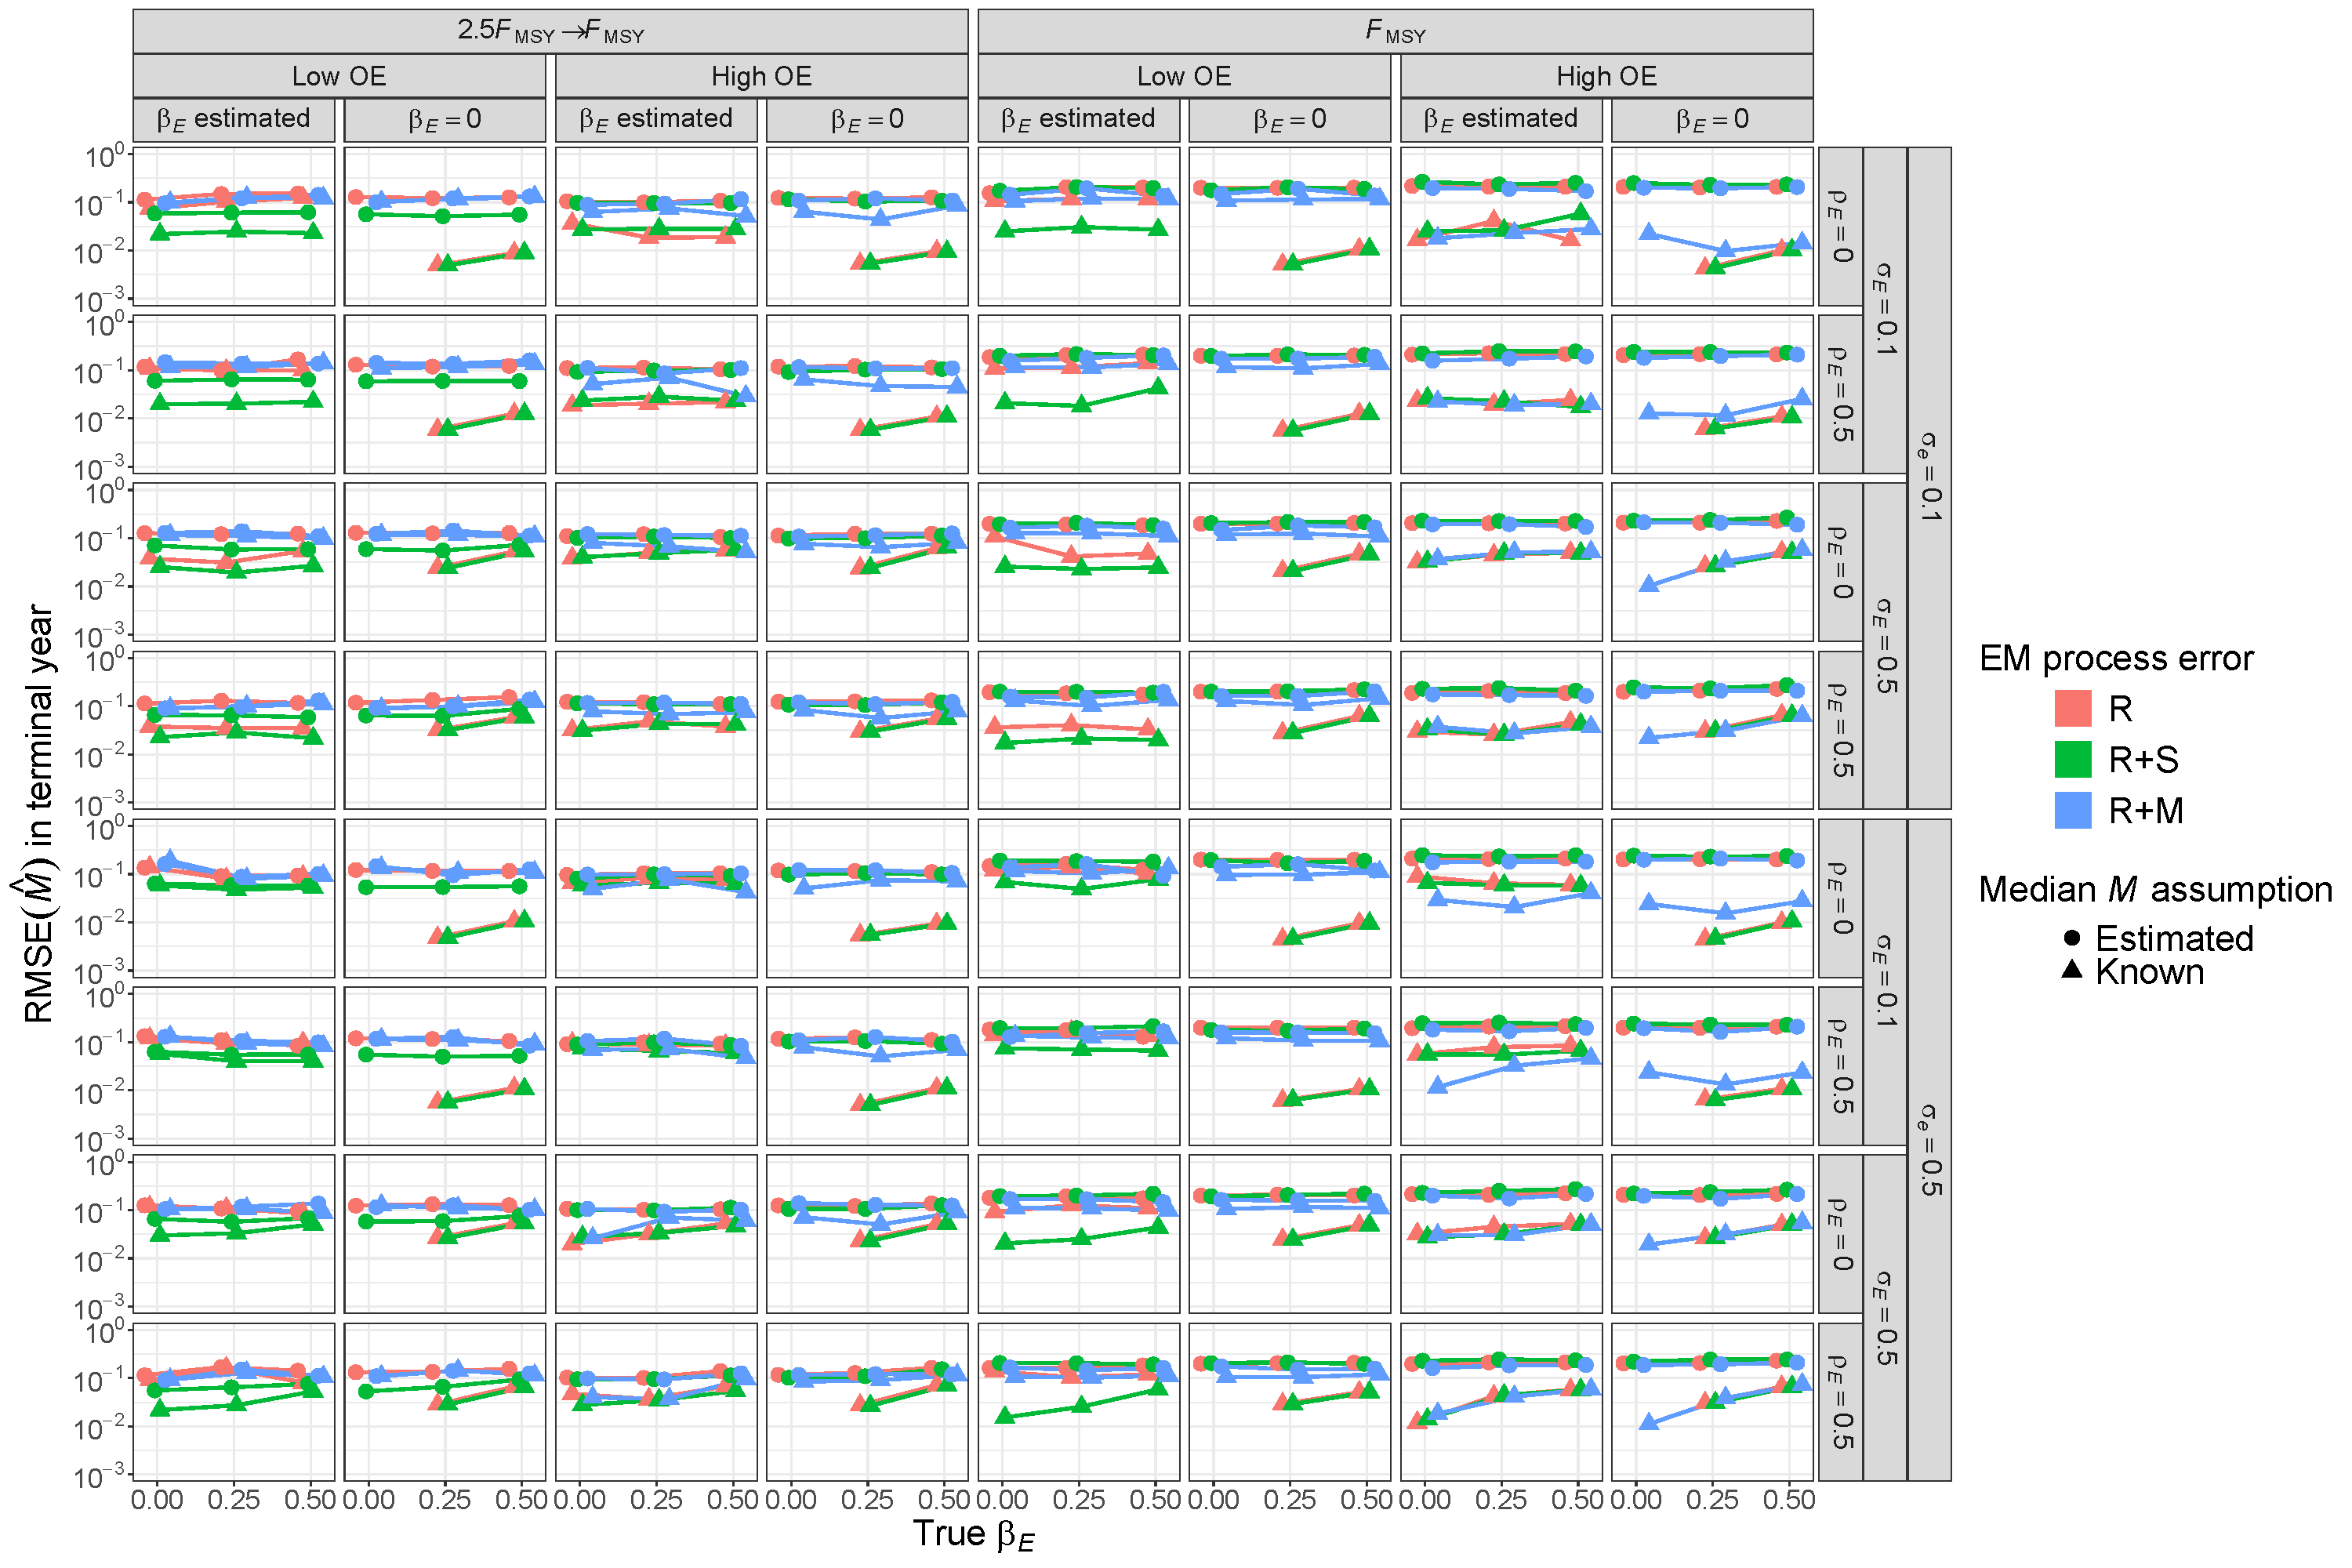
\includegraphics[height = \textheight]{terminal_year_M_rmse_RSom}
\end{center}
\caption{For R+S operating models, RMSE of estimates of terminal year $M$ for estimating models with alternative process error assumptions, treatment of covariate effect ($\beta_E = 0$ or estimated), and treatment of median $M$ parameter ($\beta_M$ estimated or known).}\label{terminal_M_rmse_RSom}
\end{figure}
\end{landscape}

\begin{landscape}
\begin{figure}
\begin{center}
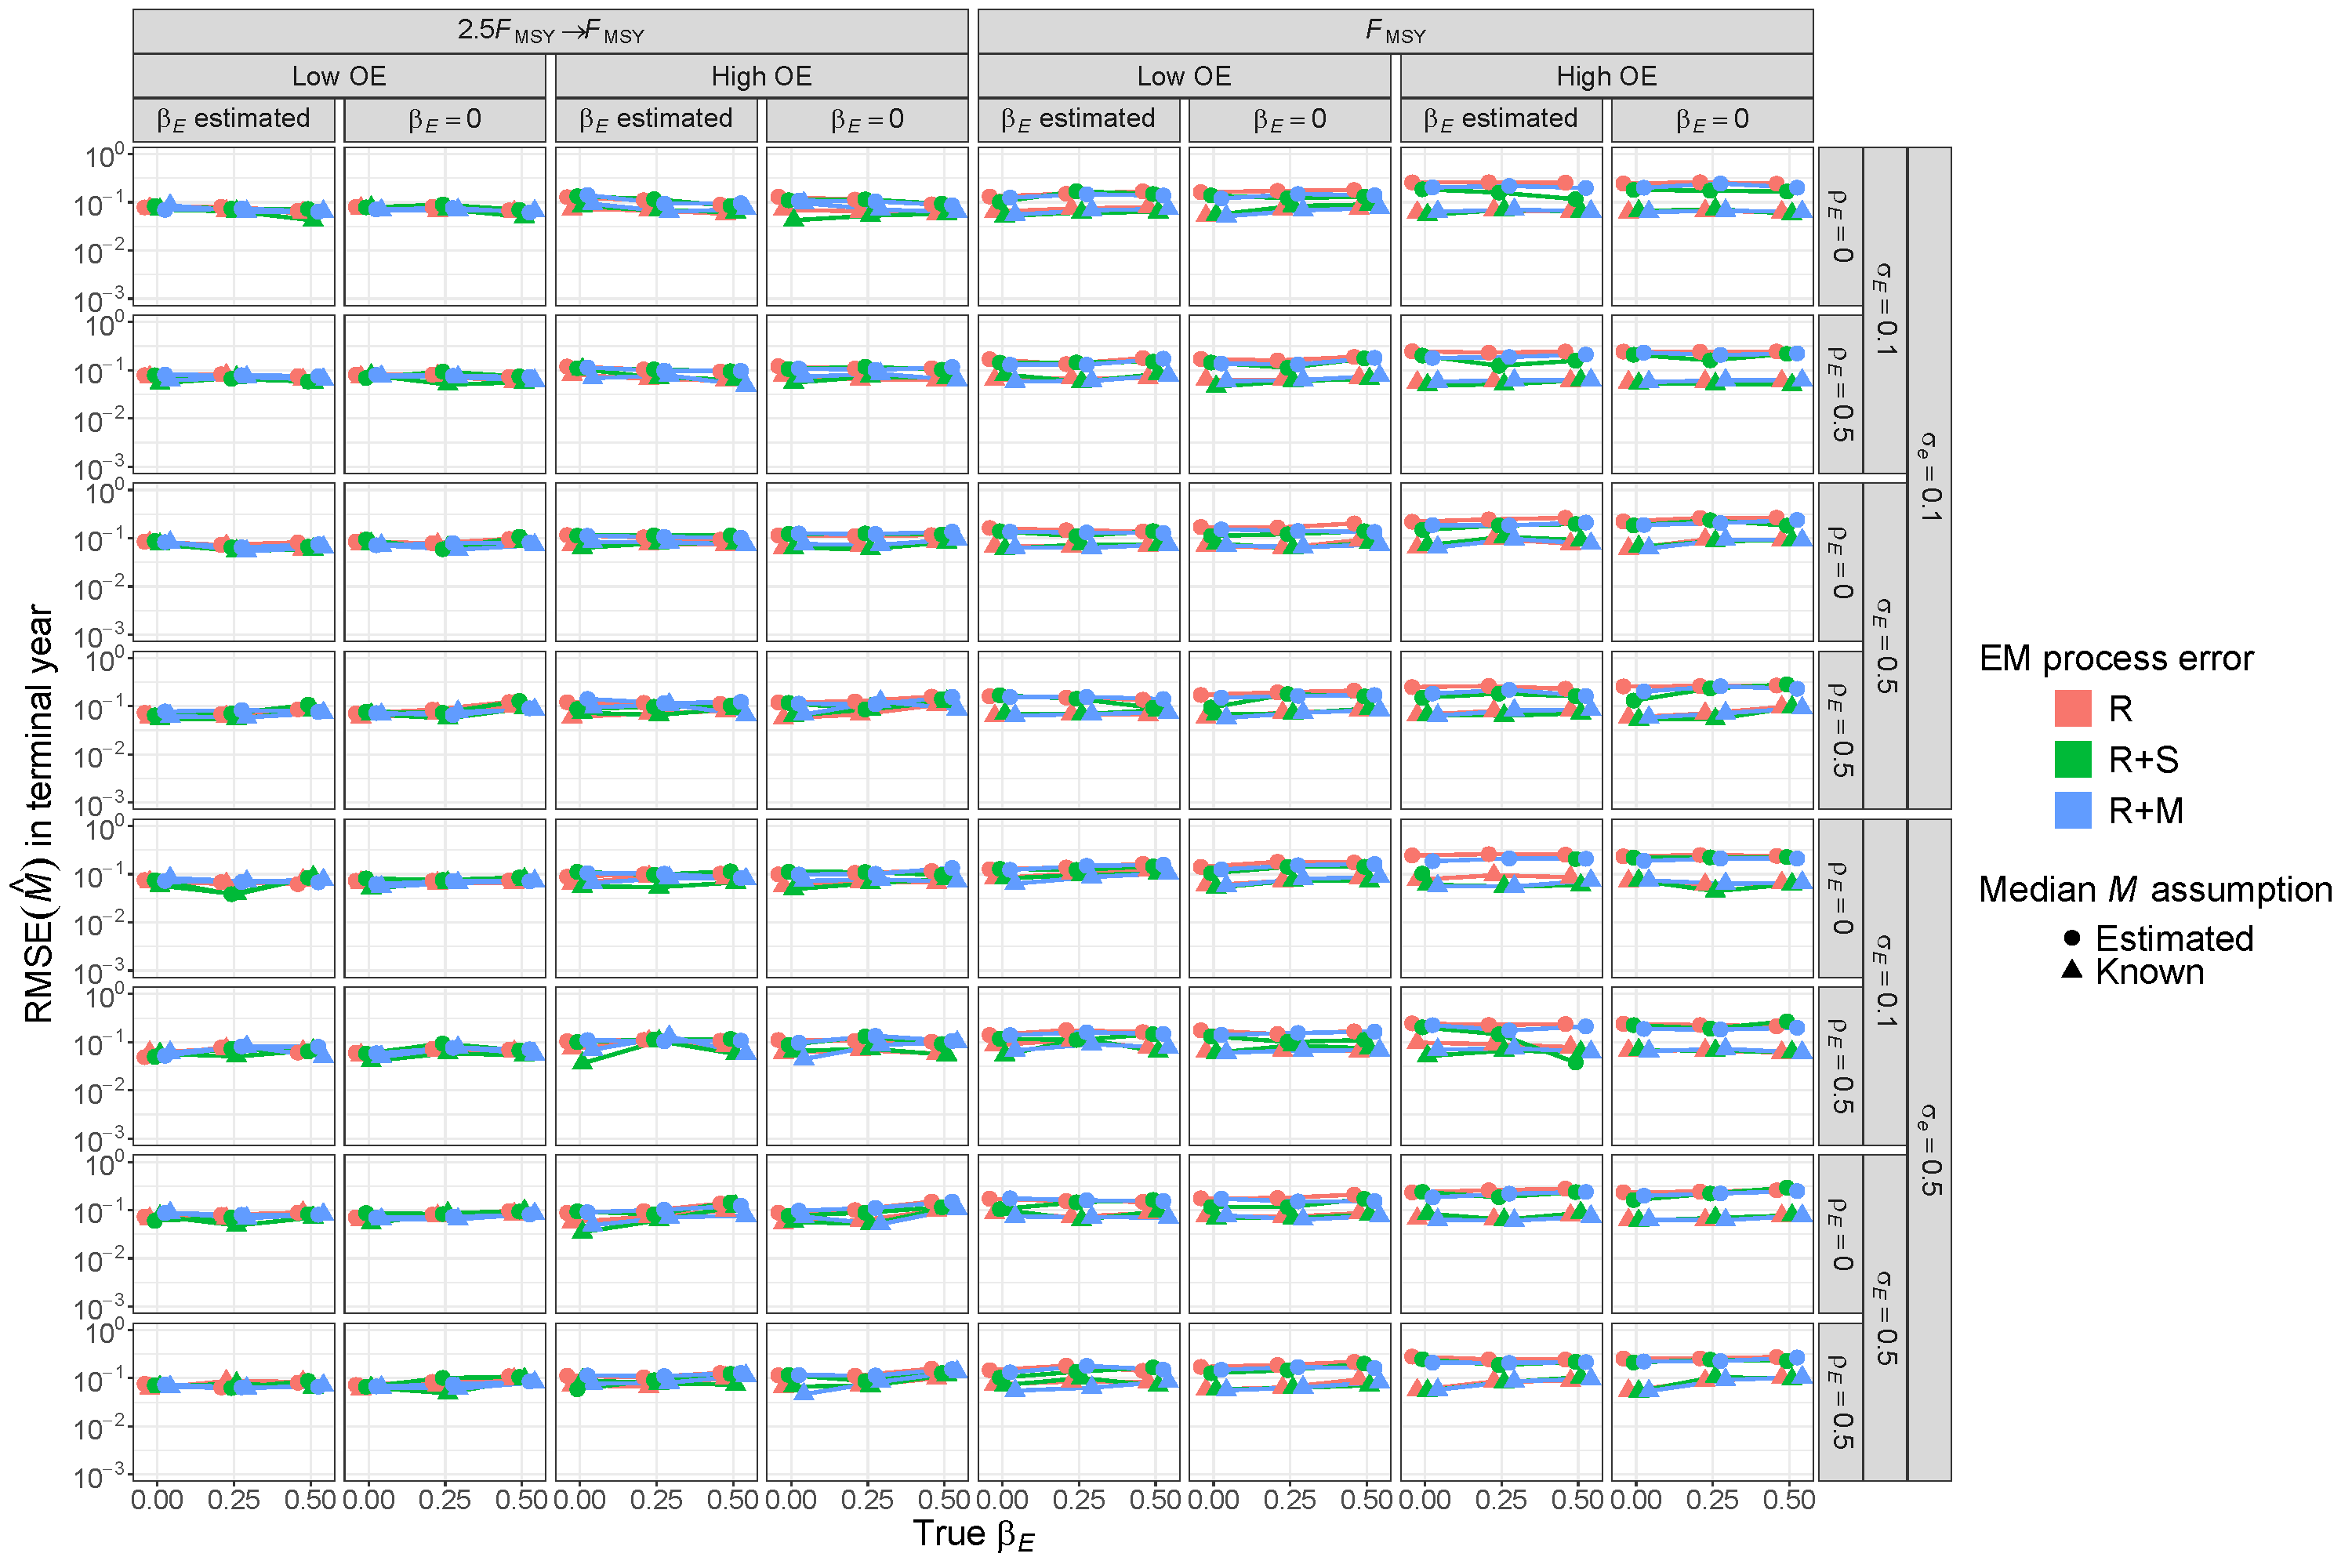
\includegraphics[height = \textheight]{terminal_year_M_rmse_RMom}
\end{center}
\caption{For R+M operating models, RMSE of estimates of terminal year $M$ for estimating models with alternative process error assumptions, treatment of covariate effect ($\beta_E = 0$ or estimated), and treatment of median $M$ parameter ($\beta_M$ estimated or known).}\label{terminal_M_rmse_RMom}
\end{figure}
\end{landscape}

\begin{landscape}
\begin{figure}
\begin{center}
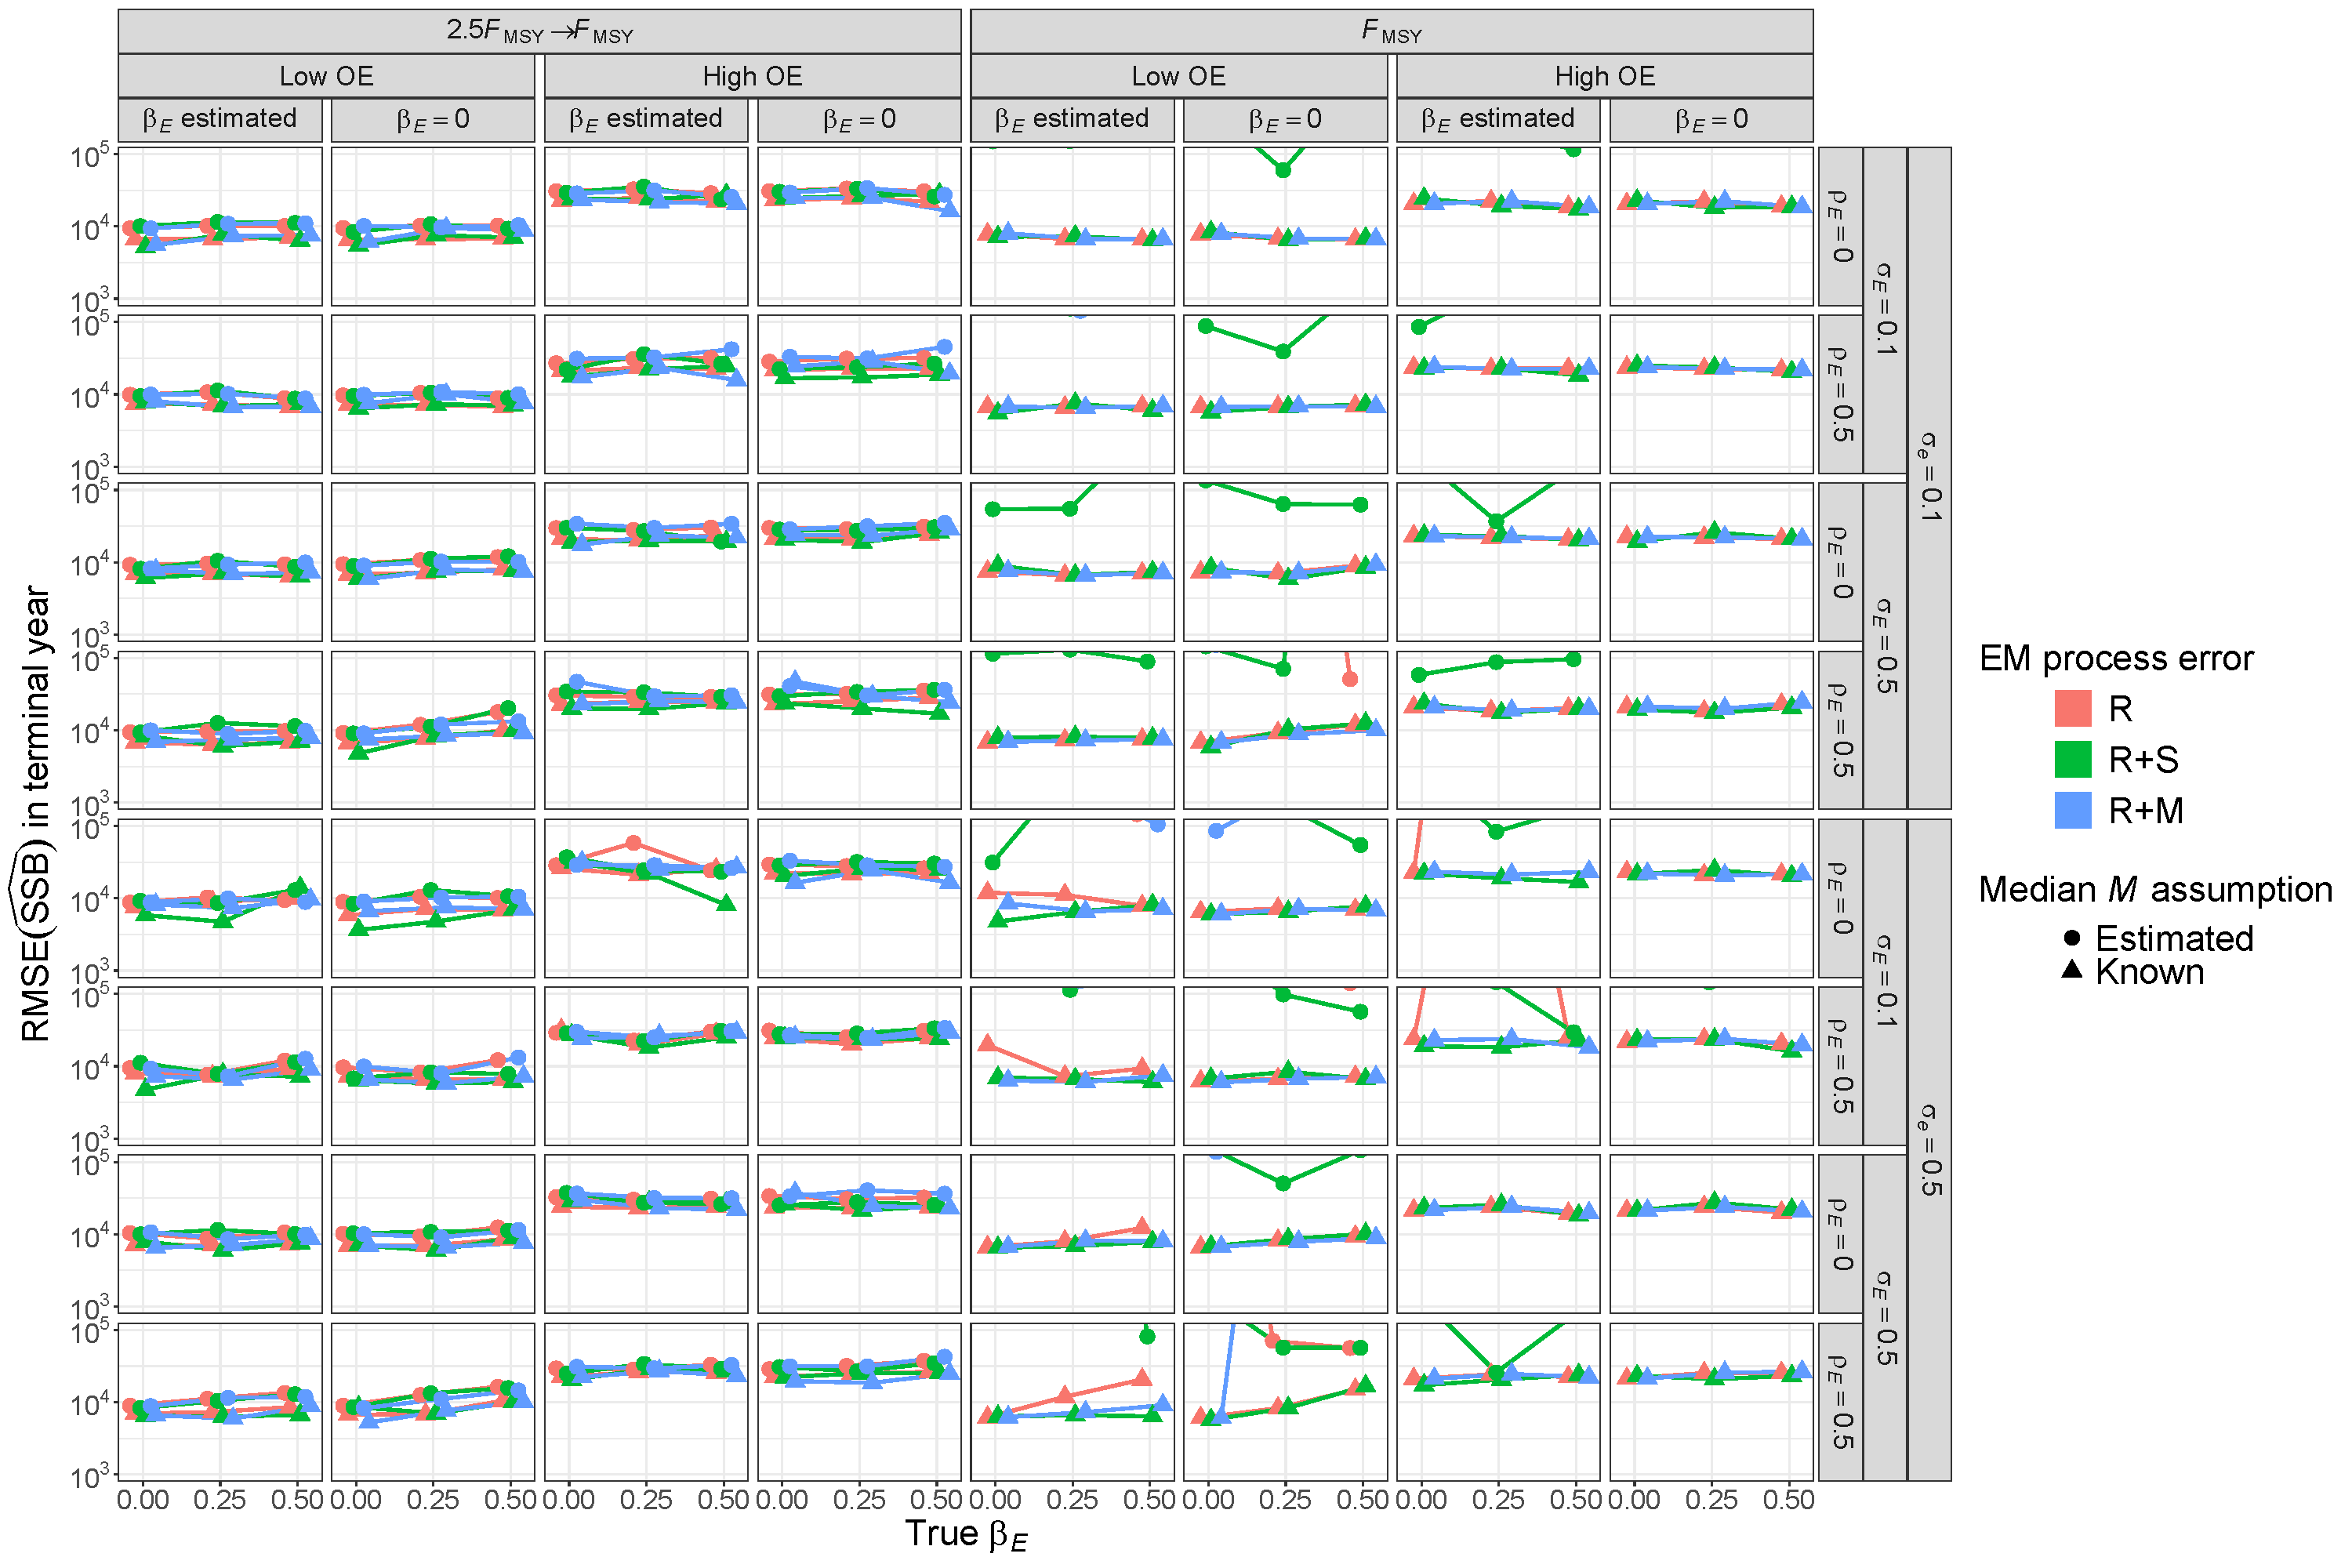
\includegraphics[height = \textheight]{terminal_year_ssb_rmse_Rom}
\end{center}
\caption{For R operating models, RMSE of estimates of SSB in the terminal year for estimating models with alternative process error assumptions, treatment of covariate effect ($\beta_E = 0$ or estimated), and treatment of median $M$ parameter ($\beta_M$ estimated or known).}\label{terminal_ssb_rmse_Rom}
\end{figure}
\end{landscape}

\begin{landscape}
\begin{figure}
\begin{center}
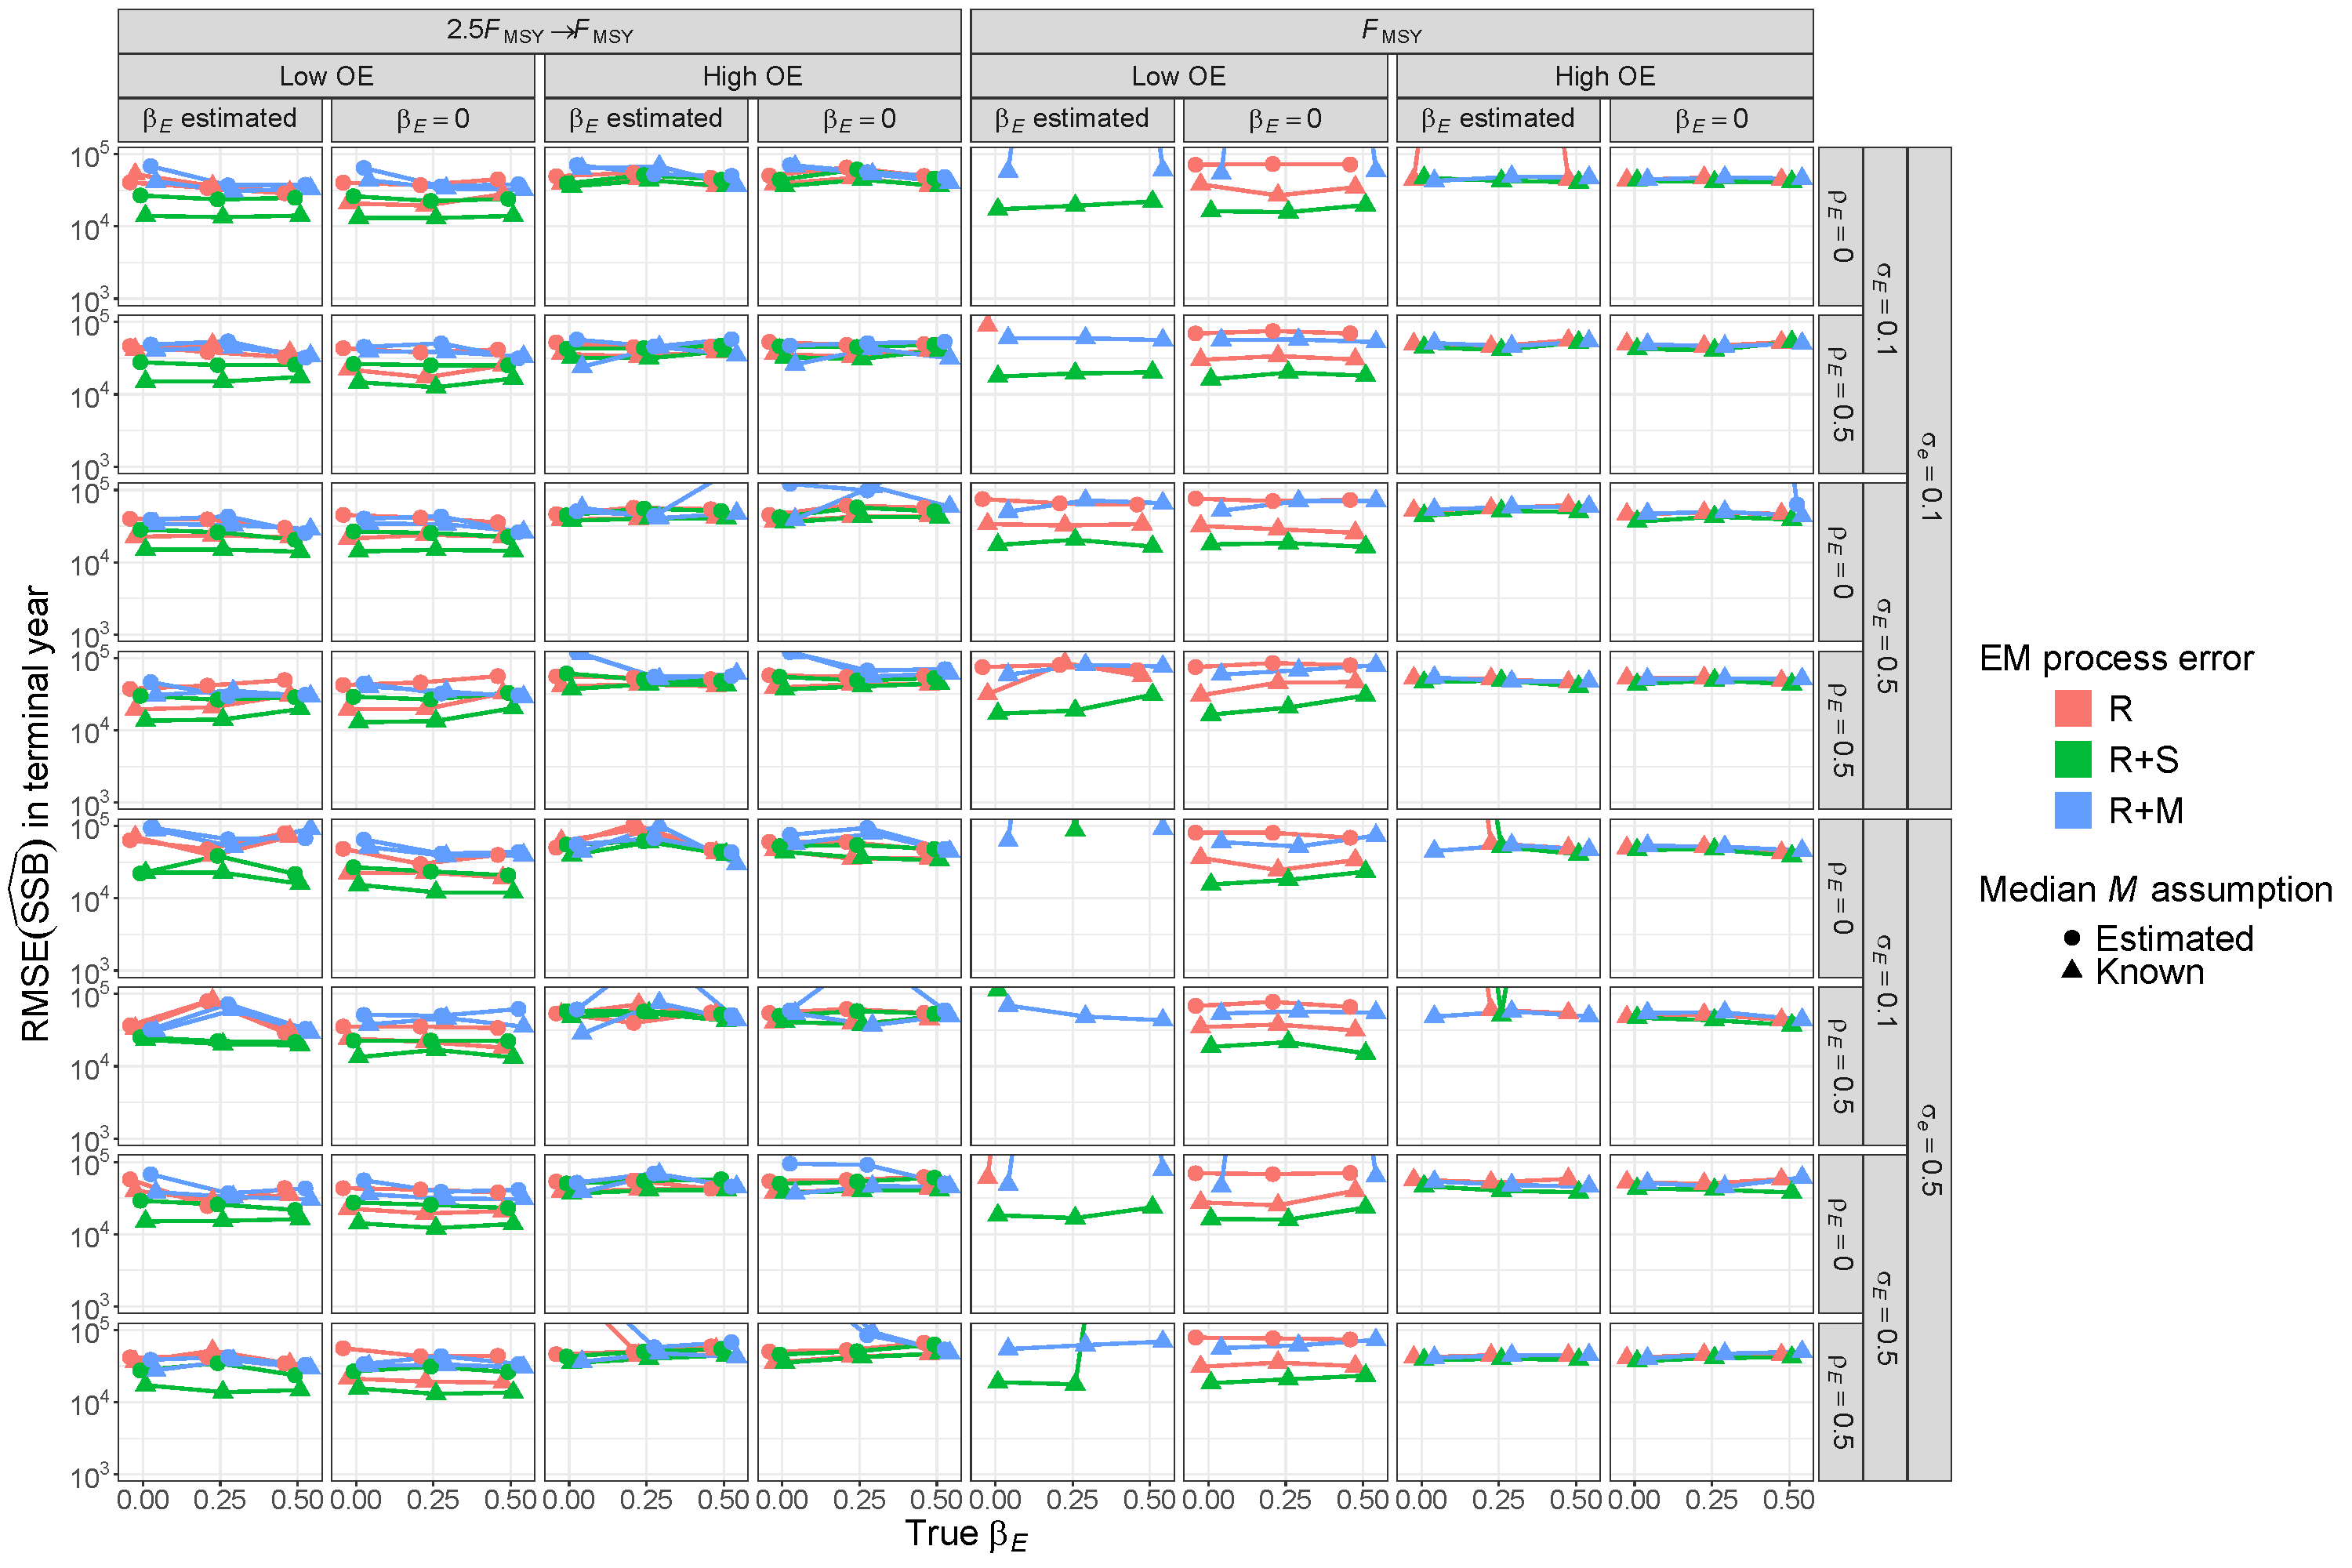
\includegraphics[height = \textheight]{terminal_year_ssb_rmse_RSom}
\end{center}
\caption{For R+S operating models, RMSE of estimates of SSB in the terminal year for estimating models with alternative process error assumptions, treatment of covariate effect ($\beta_E = 0$ or estimated), and treatment of median $M$ parameter ($\beta_M$ estimated or known).}\label{terminal_ssb_rmse_RSom}
\end{figure}
\end{landscape}

\begin{landscape}
\begin{figure}
\begin{center}
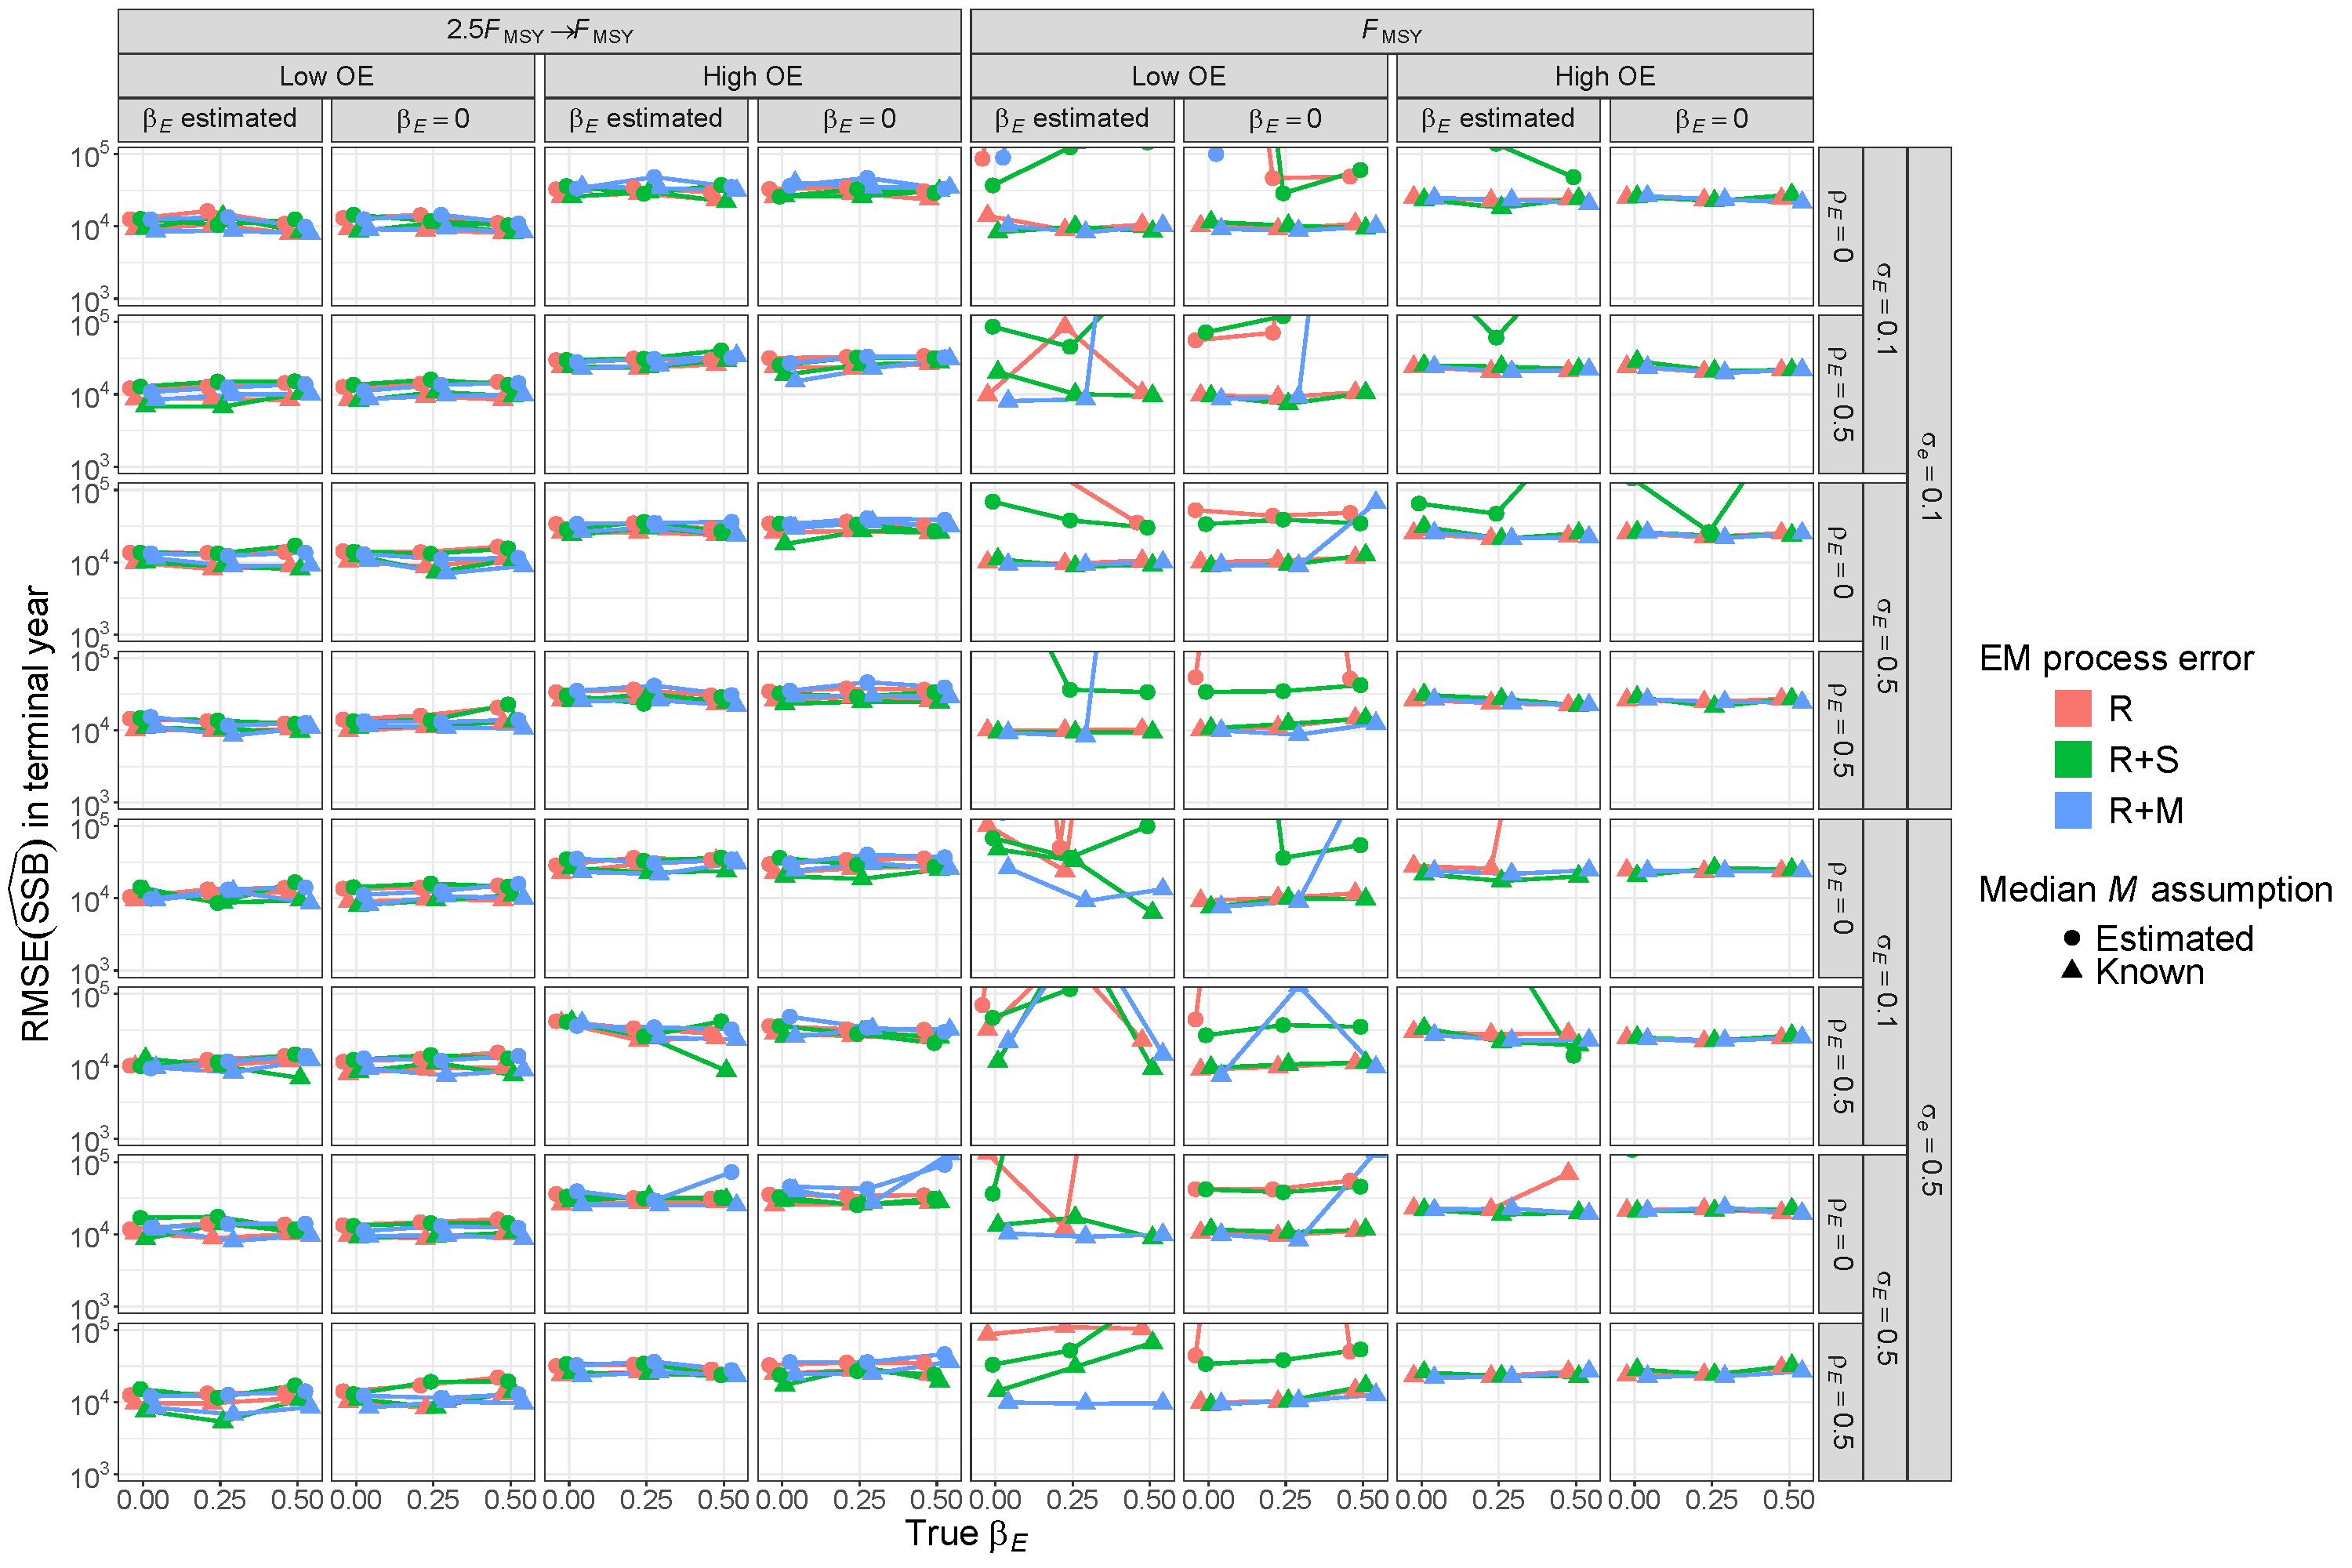
\includegraphics[height = \textheight]{terminal_year_ssb_rmse_RMom}
\end{center}
\caption{For R+M operating models, RMSE of estimates of SSB in the terminal year for estimating models with alternative process error assumptions, treatment of covariate effect ($\beta_E = 0$ or estimated), and treatment of median $M$ parameter ($\beta_M$ estimated or known).}\label{terminal_ssb_rmse_RMom}
\end{figure}
\end{landscape}

\begin{landscape}
\begin{figure}
\begin{center}
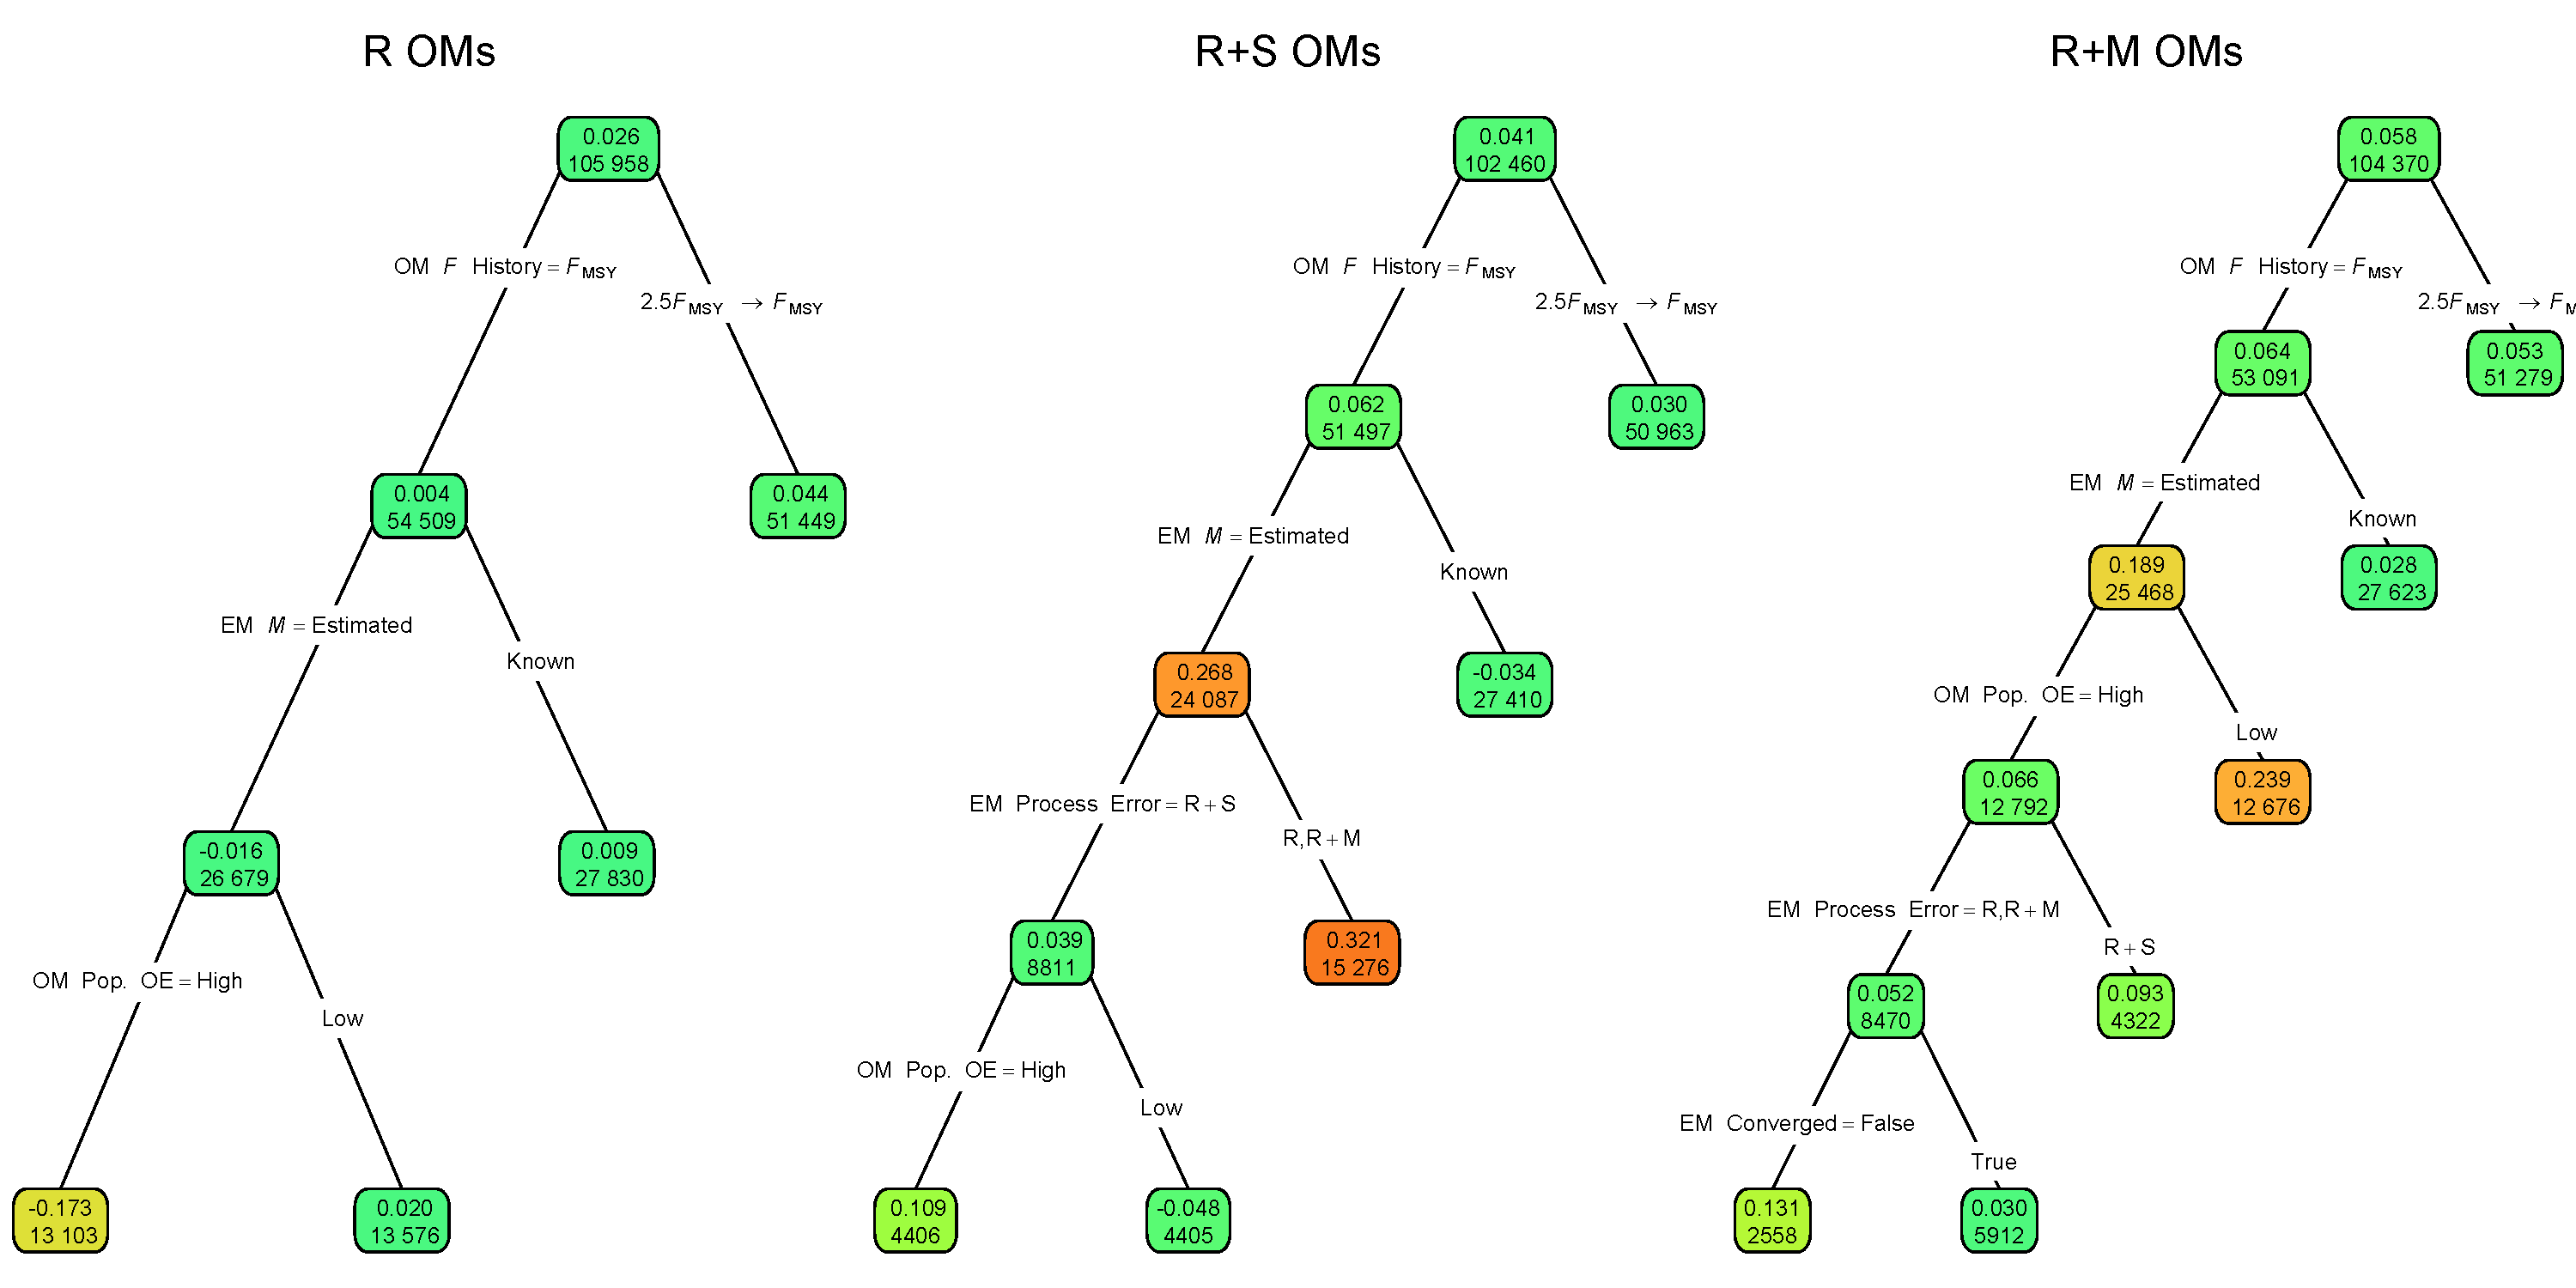
\includegraphics[width = 1.4\textwidth]{term_F_bias_regtree_plots}
\end{center}
\caption{Regression trees for errors terminal year fishing mortality rate as measured by Eq. 2. Each node shows the median error for the corresponding subset. Lower or higher absolute median errors are indicated by more green or red polygons, respectively. See Figure 1 caption and Table \ref{factor_table} for further details.}\label{term_F_bias_regtree}
\end{figure}
\end{landscape}

\begin{table}
\caption{Percent reduction in deviance for linear regression models fit to errors in terminal year fishing mortality rate as measured by Eq. 2. See Tables \ref{convergence_PRD_table} and \ref{factor_table} for further details.}\label{bias_F_PRD_table}
{\input{bias_F_PRD_table}}
\end{table}

\begin{landscape}
\begin{figure}
\begin{center}
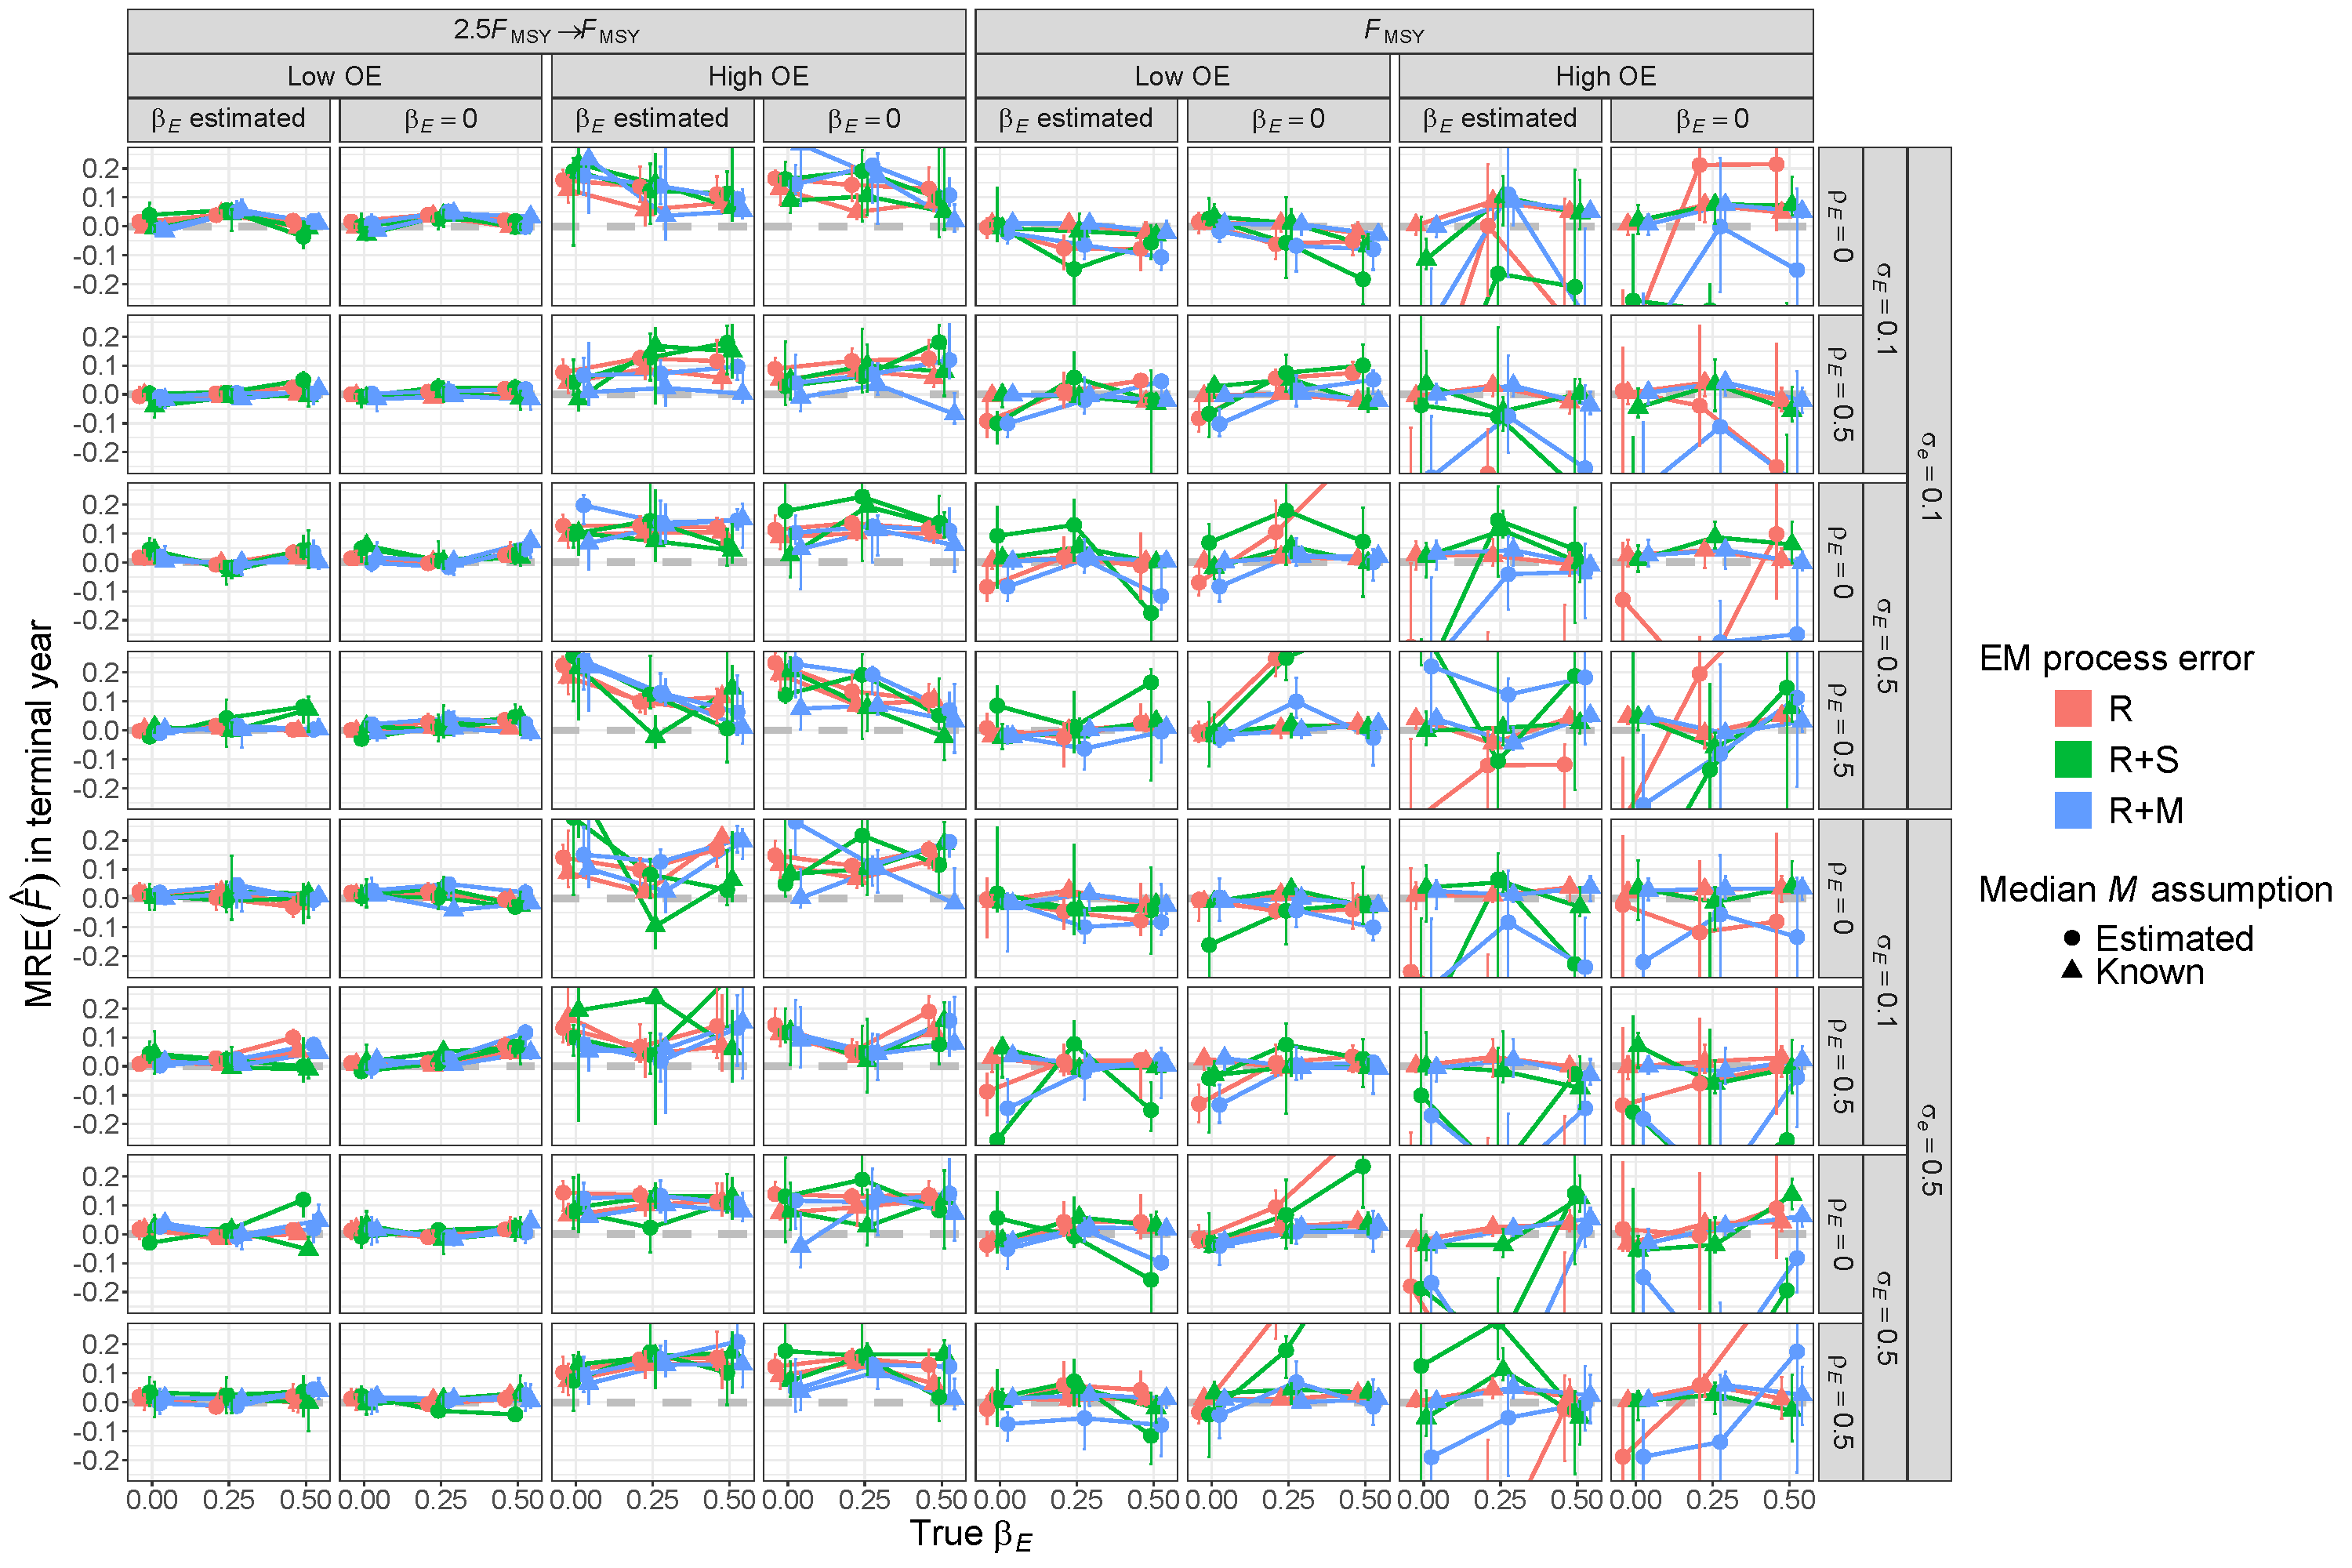
\includegraphics[height = \textheight]{terminal_year_F_bias_Rom}
\end{center}
\caption{For R operating models, median relative error (MRE) of estimates of fully-selected fishing mortality ($F$) in the terminal year for estimating models with alternative process error assumptions, treatment of covariate effect ($\beta_E = 0$ or estimated), and treatment of median $M$ parameter ($\beta_M$ estimated or known).}\label{terminal_F_bias_Rom}
\end{figure}
\end{landscape}

\begin{landscape}
\begin{figure}
\begin{center}
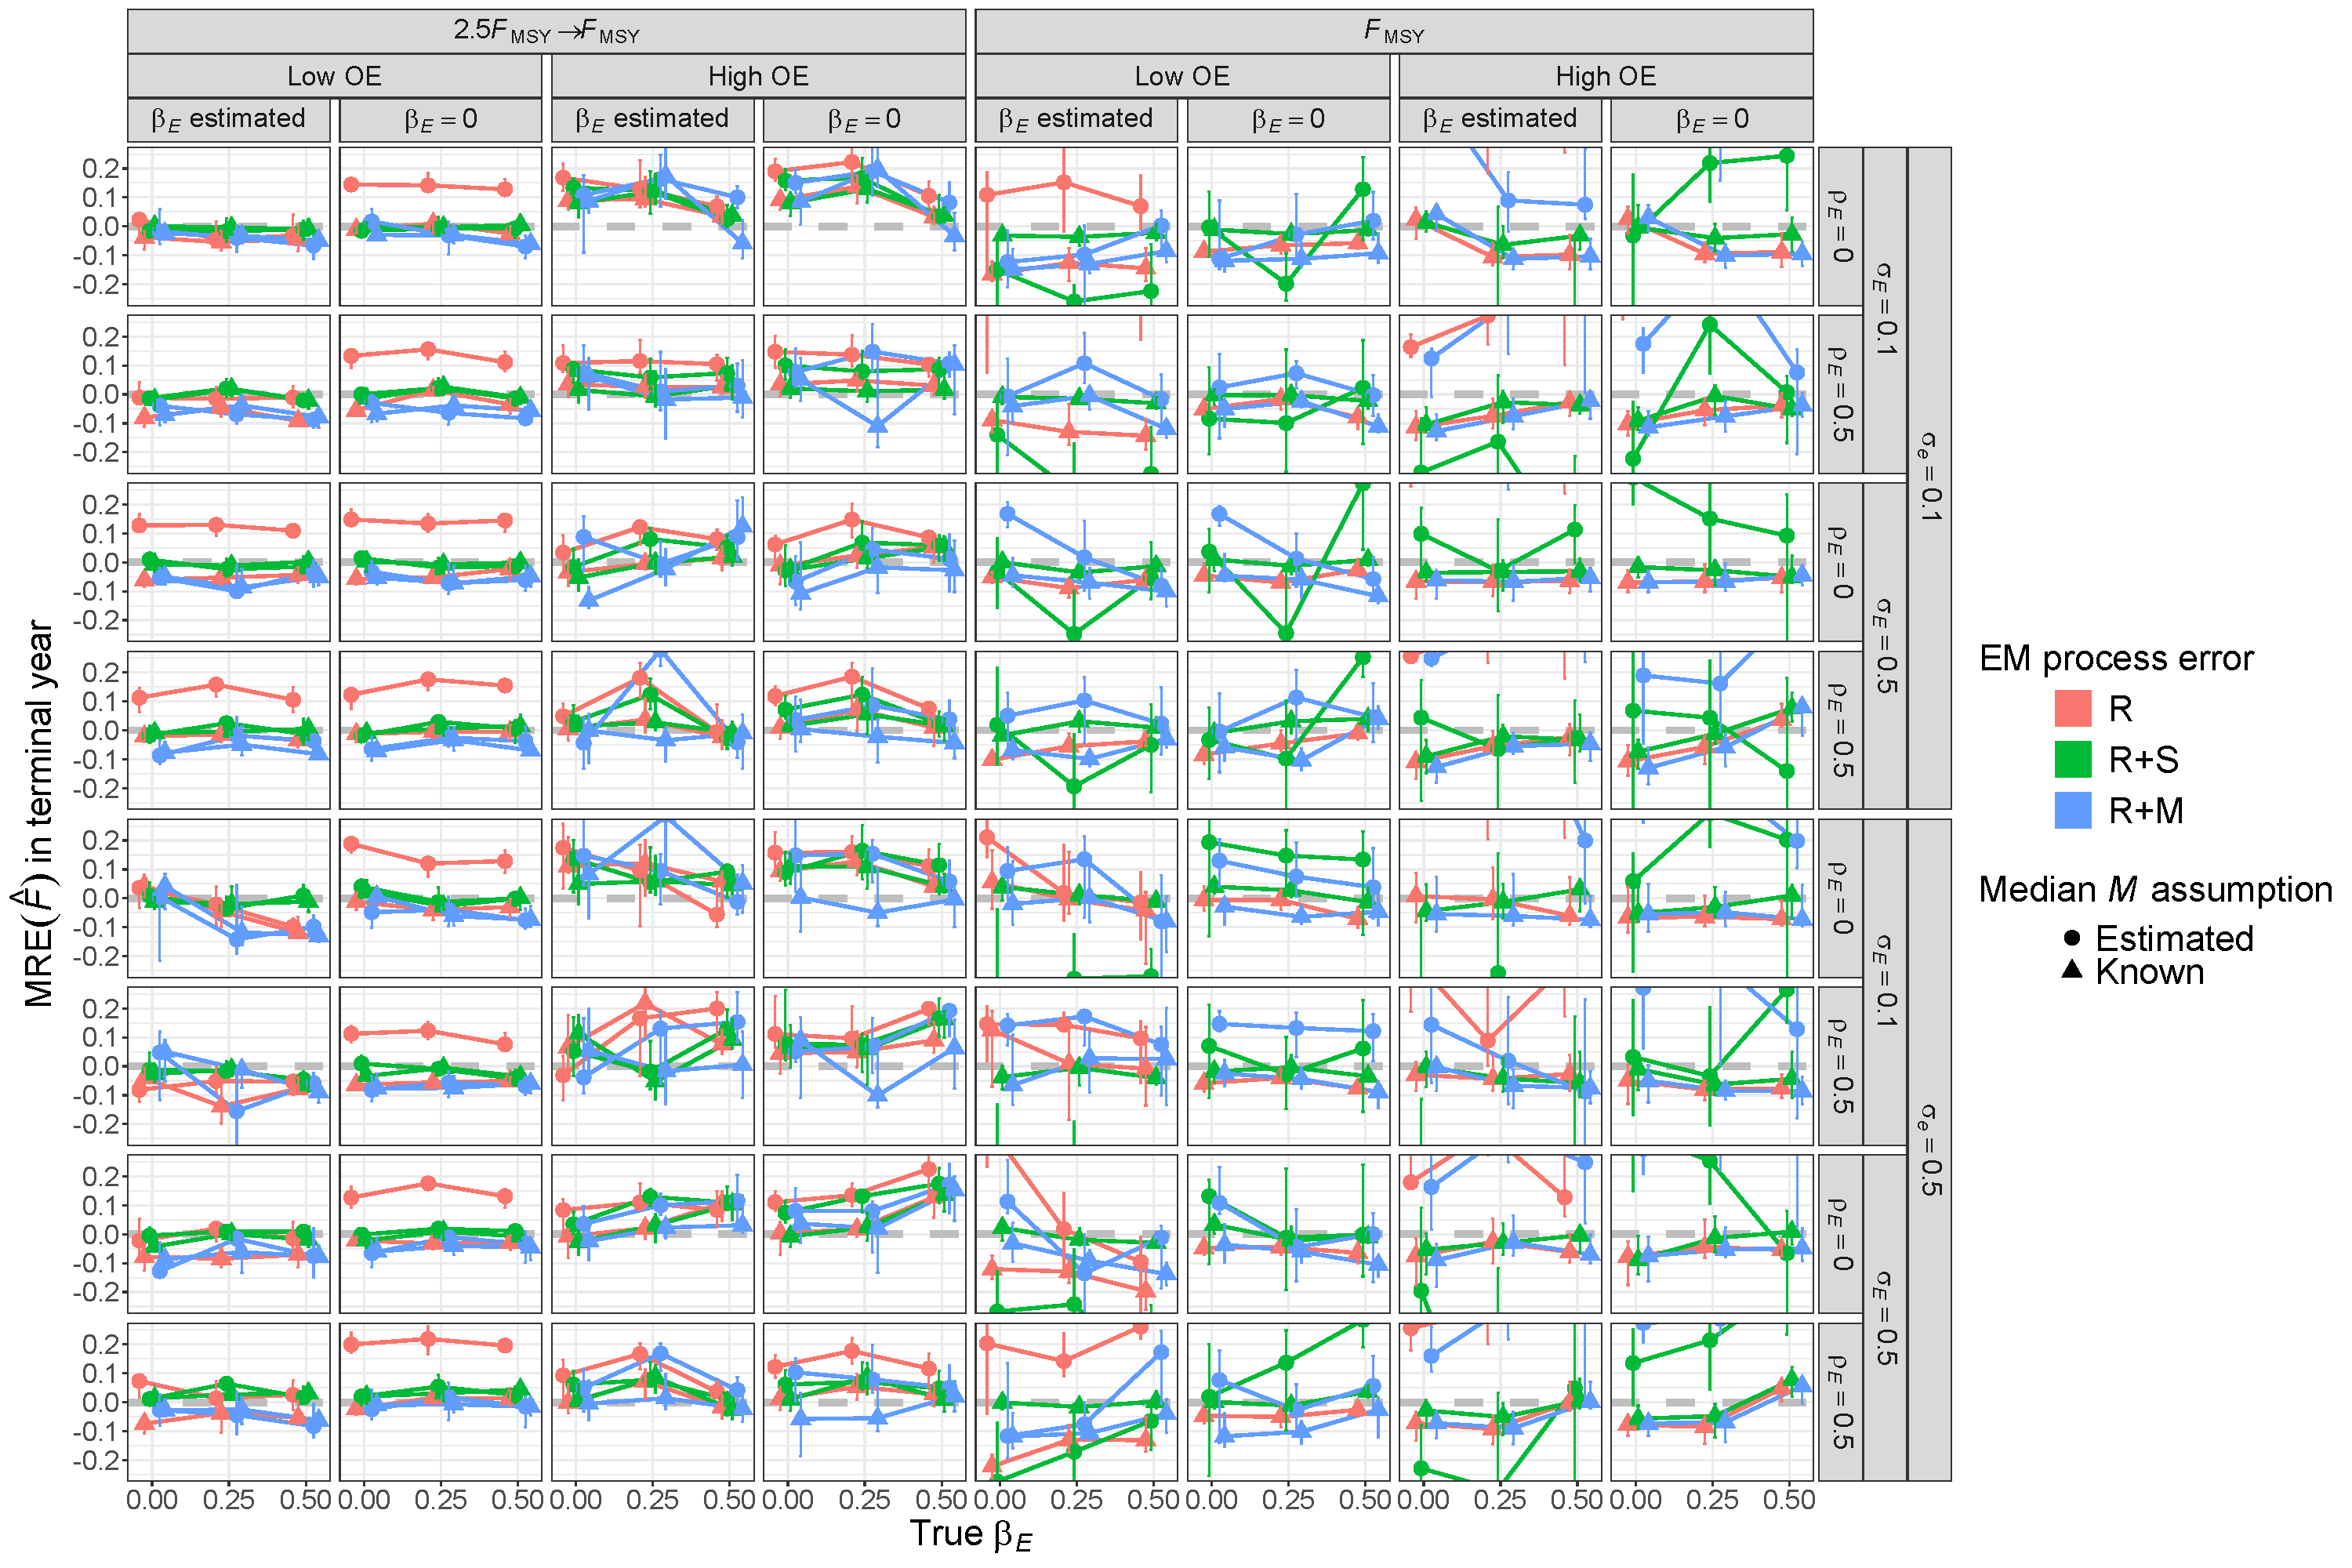
\includegraphics[height = \textheight]{terminal_year_F_bias_RSom}
\end{center}
\caption{For R+S operating models, median relative error (MRE) of estimates of fully-selected fishing mortality ($F$) in the terminal year for estimating models with alternative process error assumptions, treatment of covariate effect ($\beta_E = 0$ or estimated), and treatment of median $M$ parameter ($\beta_M$ estimated or known).}\label{terminal_F_bias_RSom}
\end{figure}
\end{landscape}

\begin{landscape}
\begin{figure}
\begin{center}
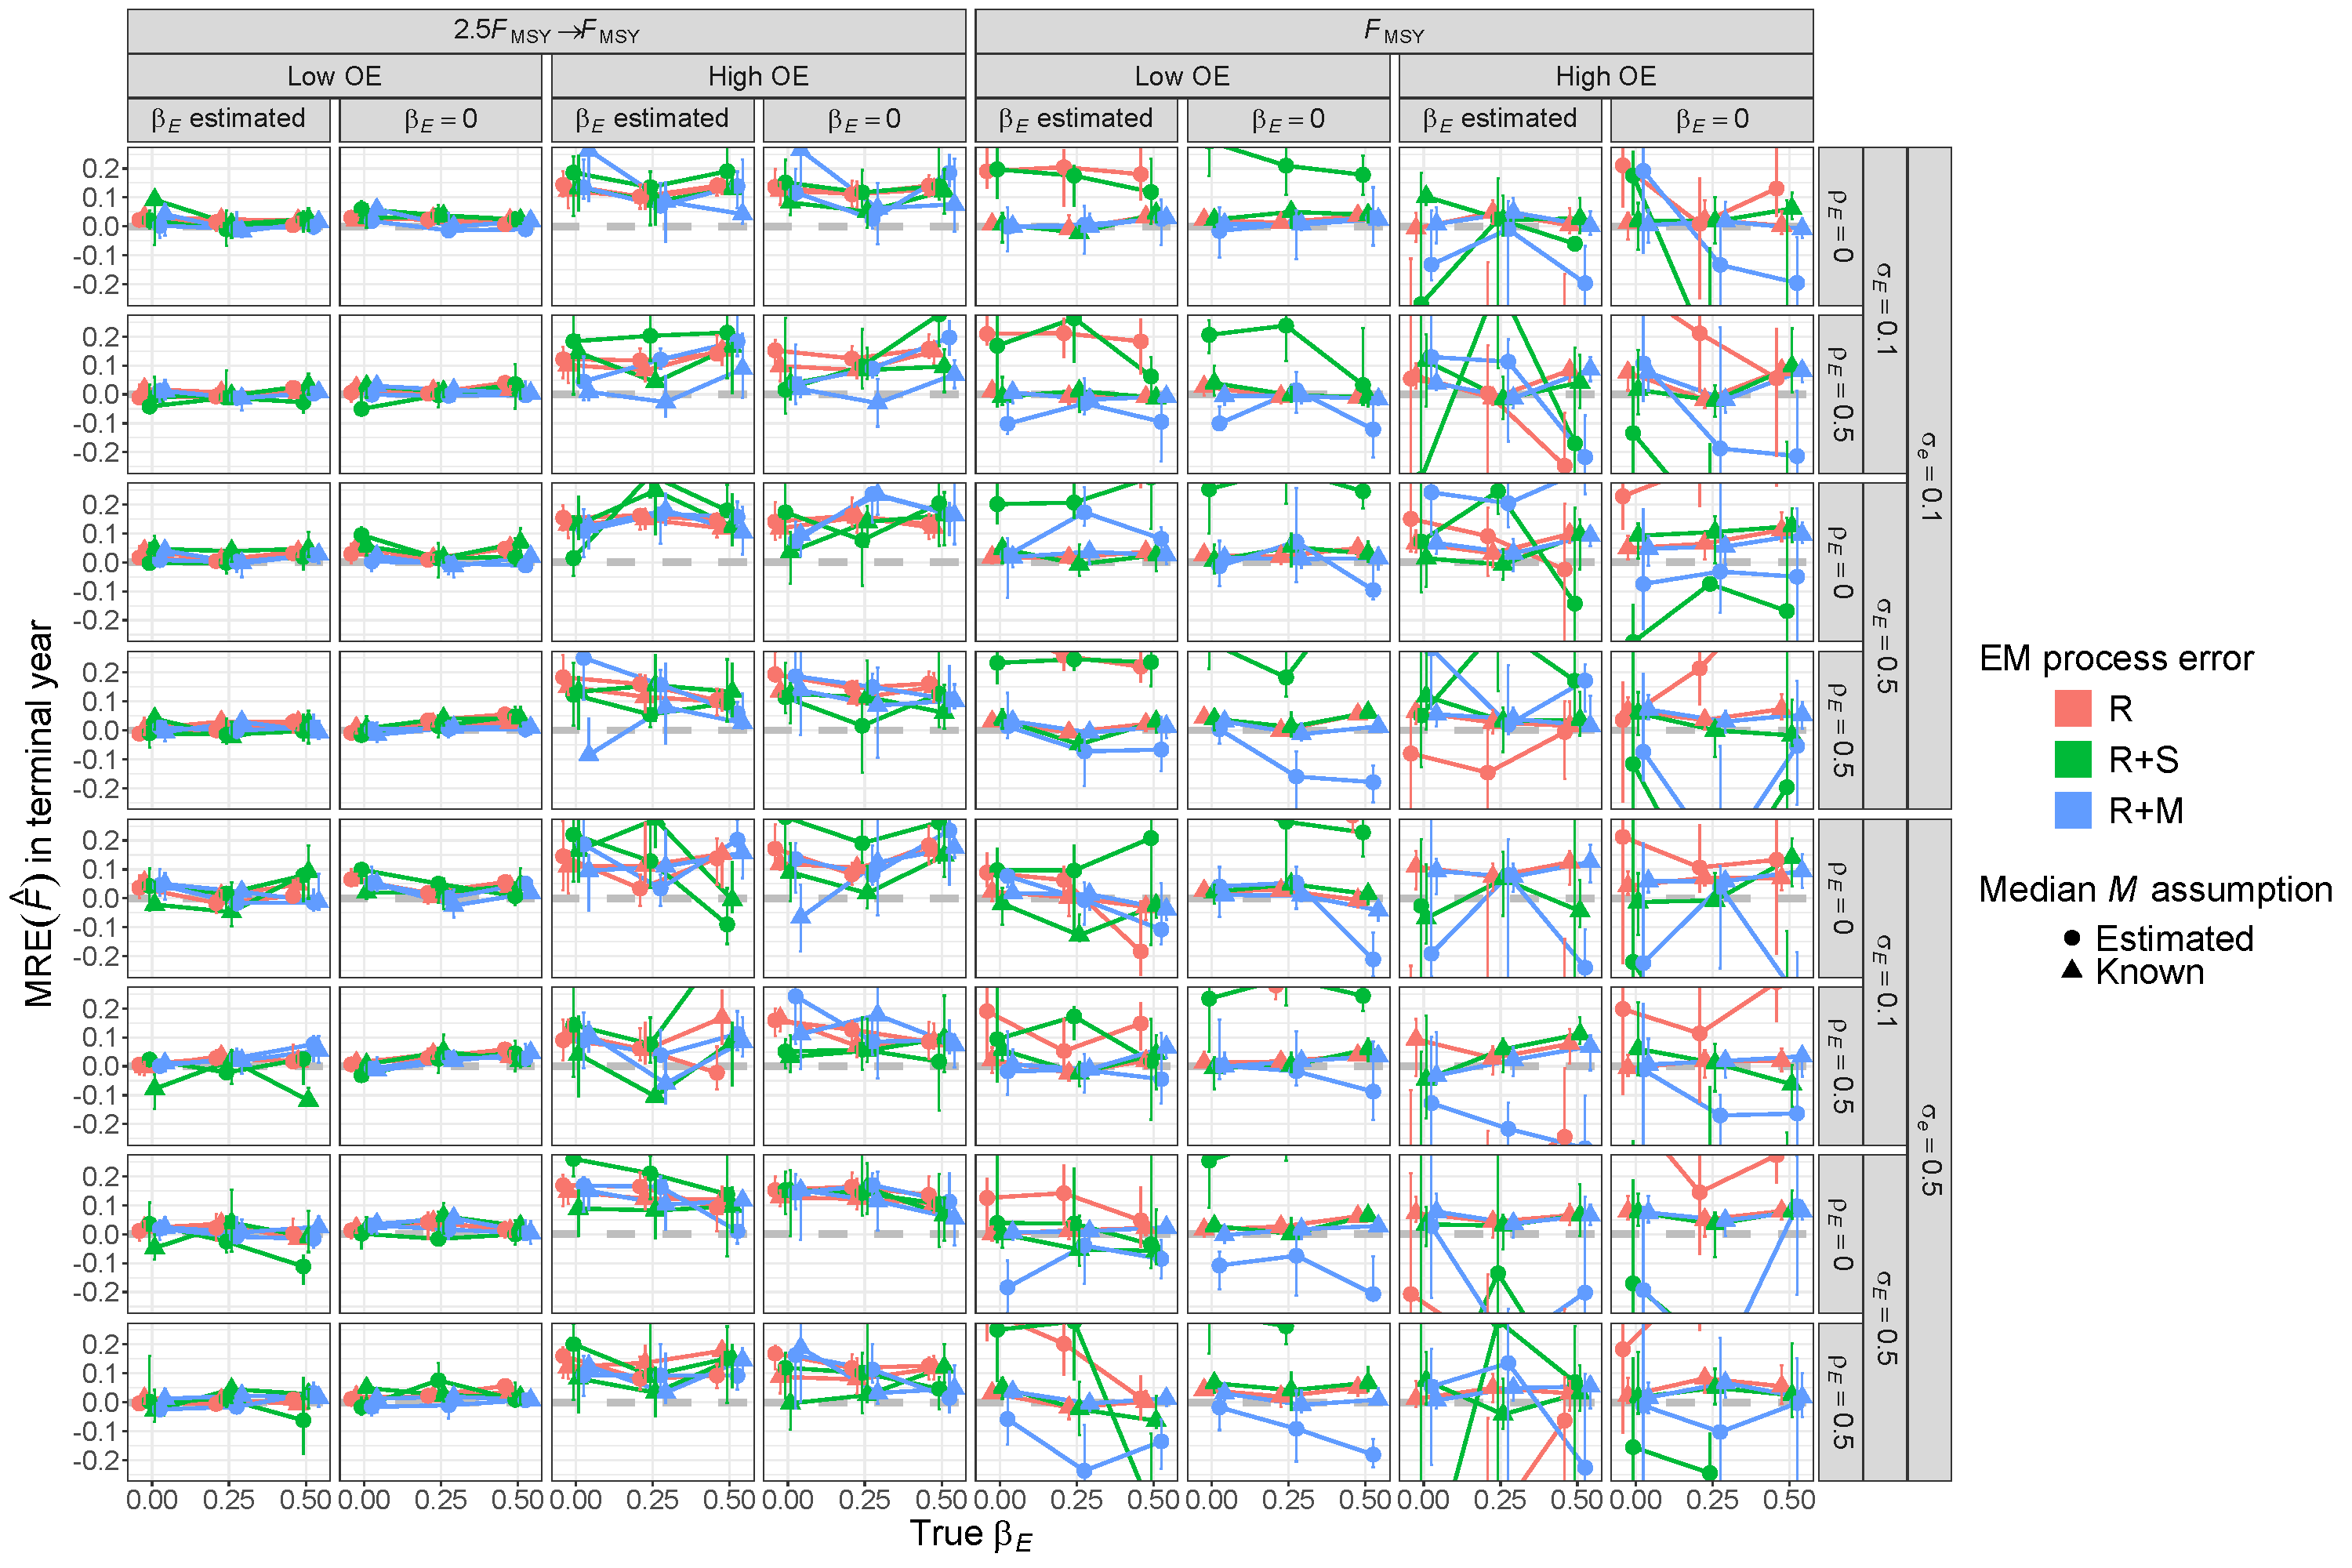
\includegraphics[height = \textheight]{terminal_year_F_bias_RMom}
\end{center}
\caption{For R+M operating models, median relative error (MRE) of estimates of fully-selected fishing mortality ($F$) in the terminal year for estimating models with alternative process error assumptions, treatment of covariate effect ($\beta_E = 0$ or estimated), and treatment of median $M$ parameter ($\beta_M$ estimated or known).}\label{terminal_F_bias_RMom}
\end{figure}
\end{landscape}

\begin{landscape}
\begin{figure}
\begin{center}
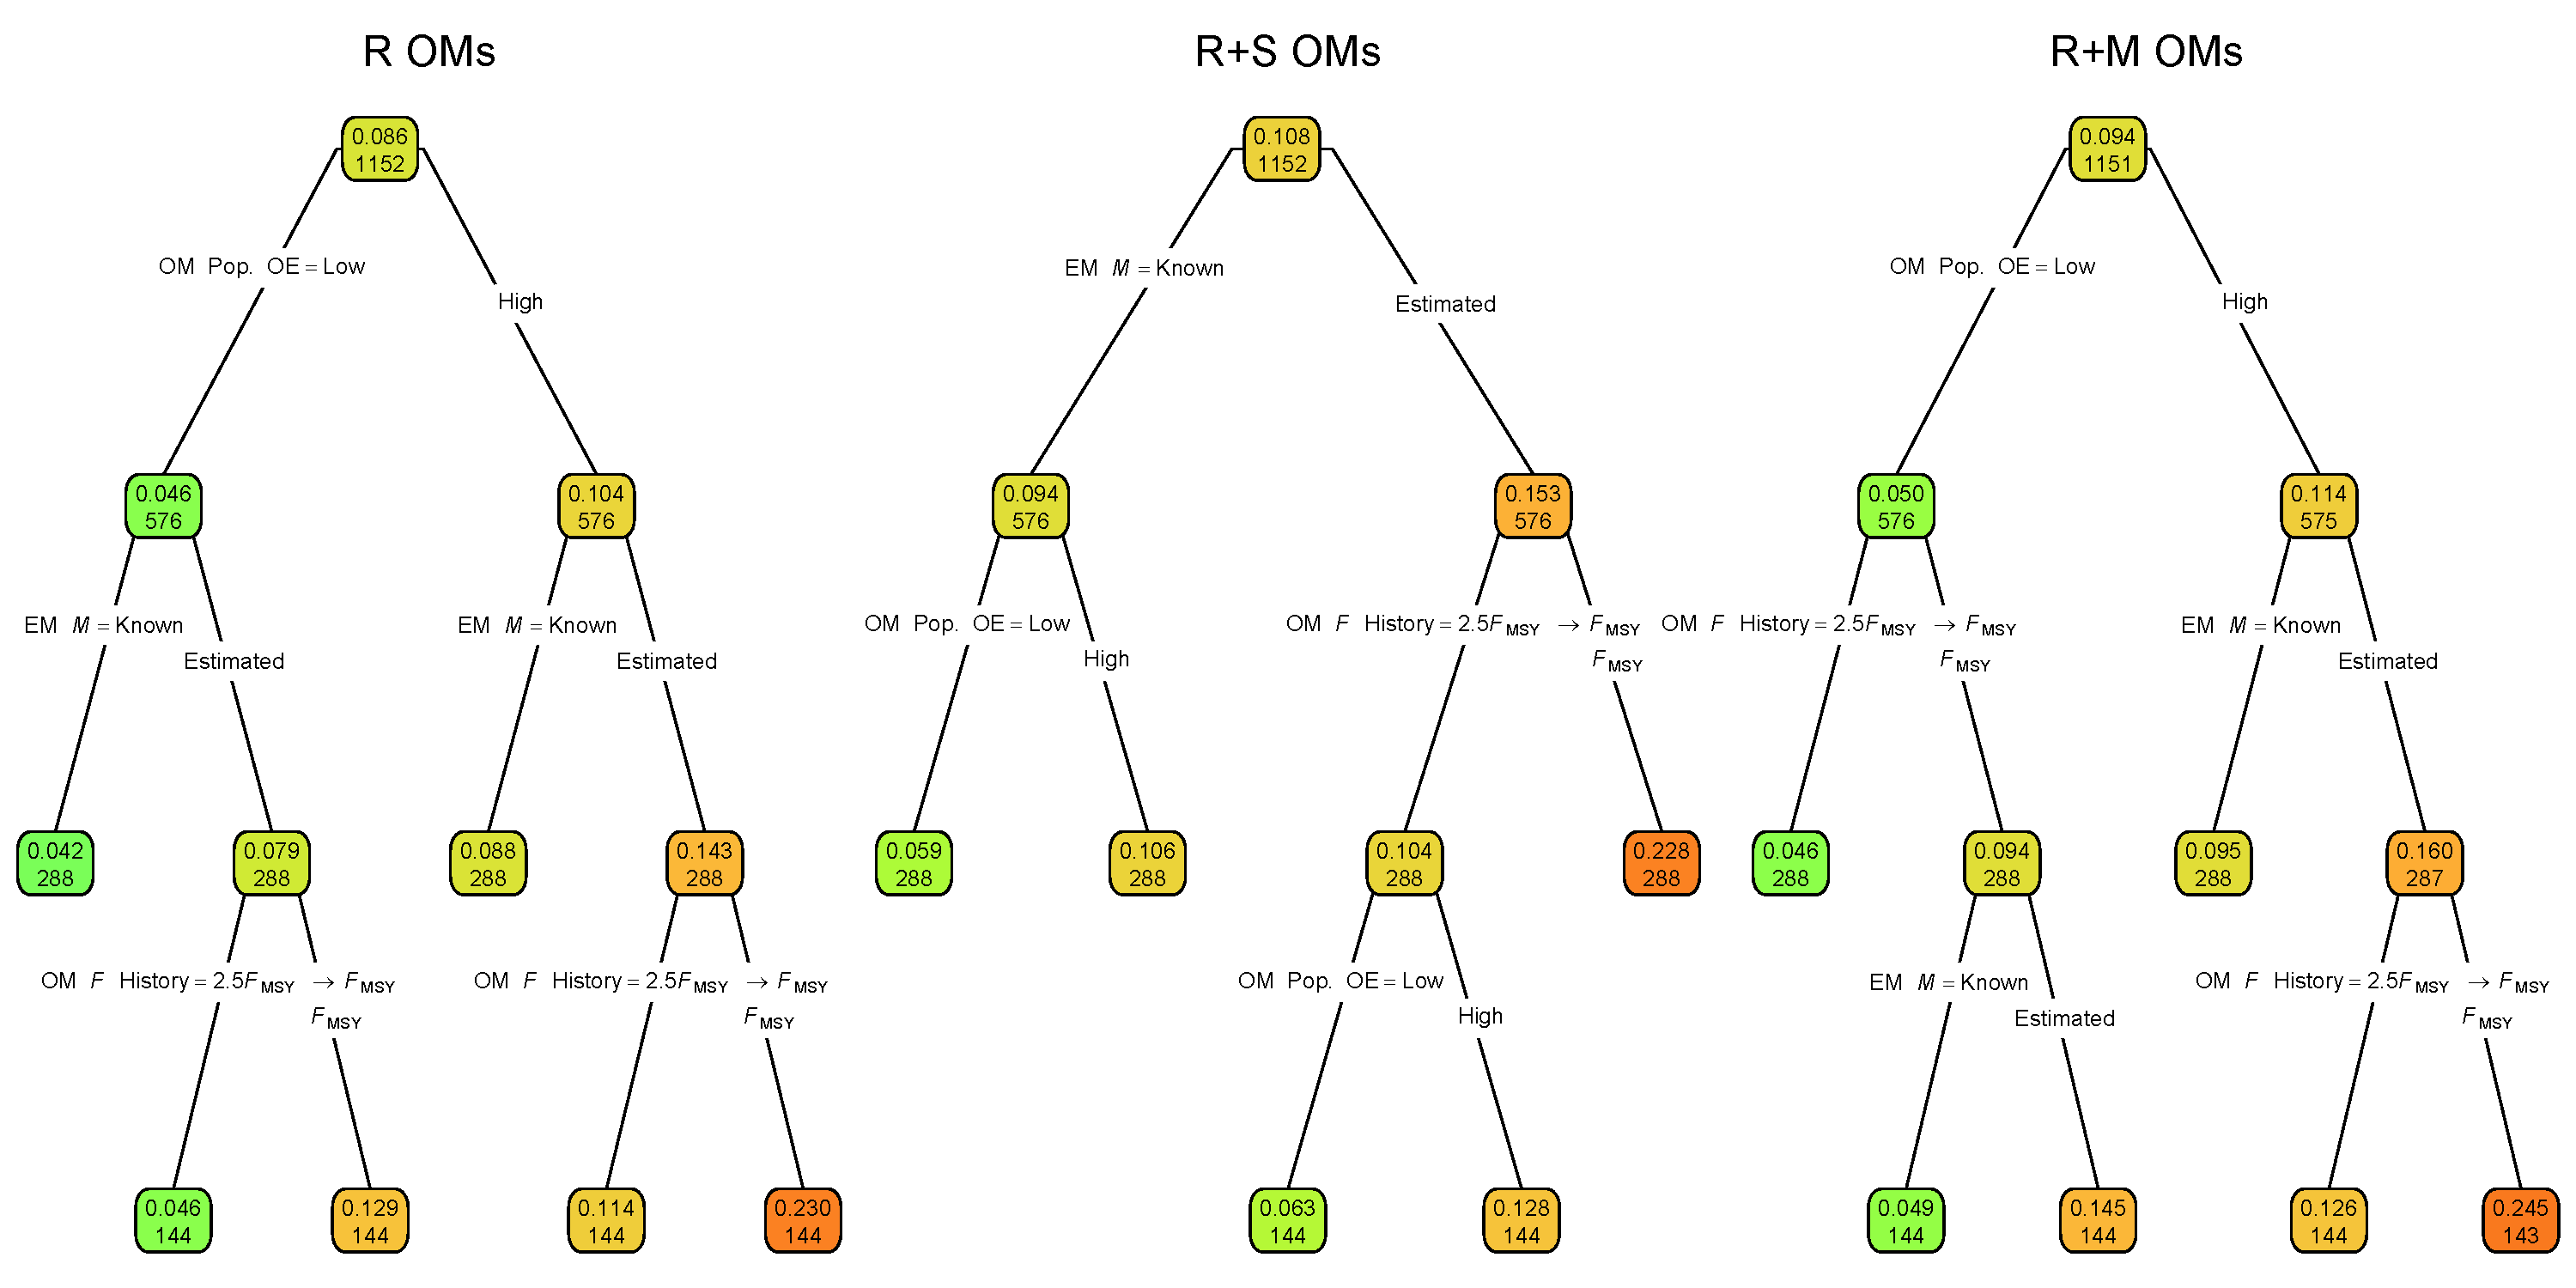
\includegraphics[width = 1.4\textwidth]{term_F_rmse_regtree_plots}
\end{center}
\caption{Regression trees for the log-transformed RMSE of terminal year fishing mortality rate. Each node shows the median error for the corresponding subset. Lower or higher median RMSE is indicated by more green or red polygons, respectively. See Figure 1 caption and Table \ref{factor_table} for further details.}\label{term_F_rmse_regtree}
\end{figure}
\end{landscape}

\begin{table}
\caption{Percent reduction in deviance for linear regression models fit to log-transformed RMSE of terminal year fishing mortality rate. See Tables \ref{convergence_PRD_table} and \ref{factor_table} for further details.}\label{rmse_F_PRD_table}
{\input{rmse_F_PRD_table}}
\end{table}
\pagebreak

\begin{landscape}
\begin{figure}
\begin{center}
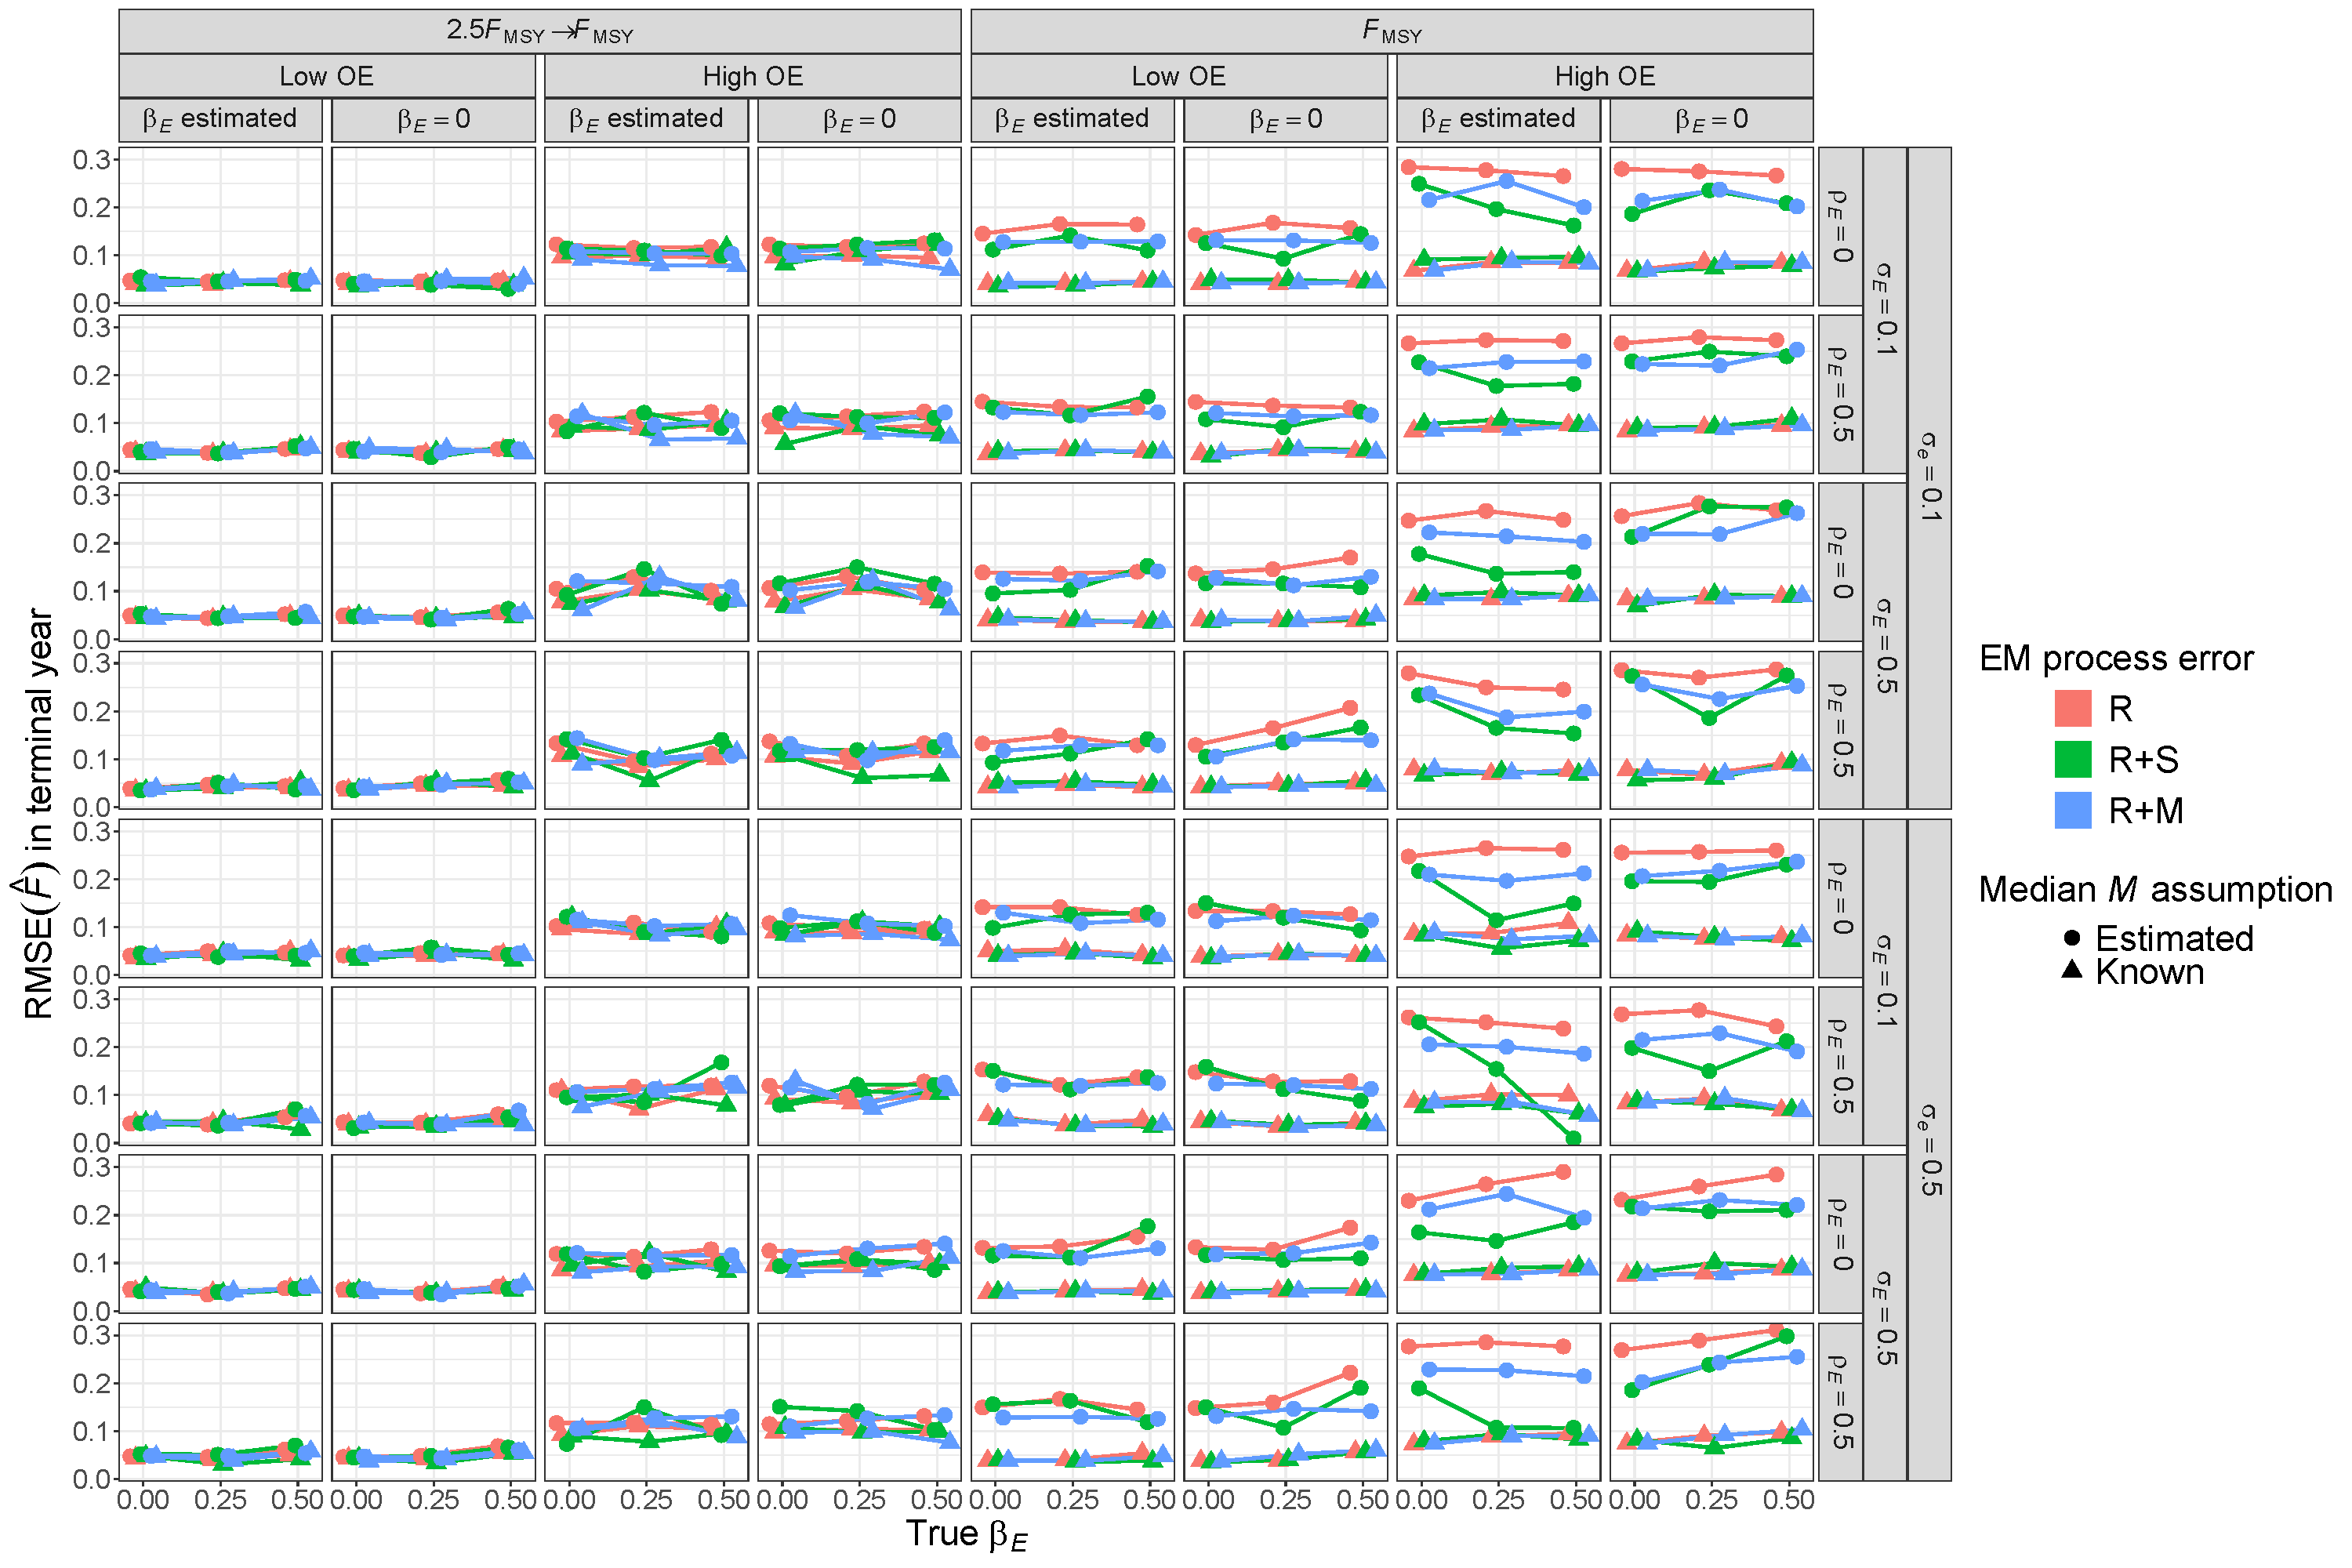
\includegraphics[height = \textheight]{terminal_year_F_rmse_Rom}
\end{center}
\caption{For R operating models, RMSE of estimates of fully-selected fishing mortality ($F$)  in the terminal year for estimating models with alternative process error assumptions, treatment of covariate effect ($\beta_E = 0$ or estimated), and treatment of median $M$ parameter ($\beta_M$ estimated or known).}\label{terminal_F_rmse_Rom}
\end{figure}
\end{landscape}

\begin{landscape}
\begin{figure}
\begin{center}
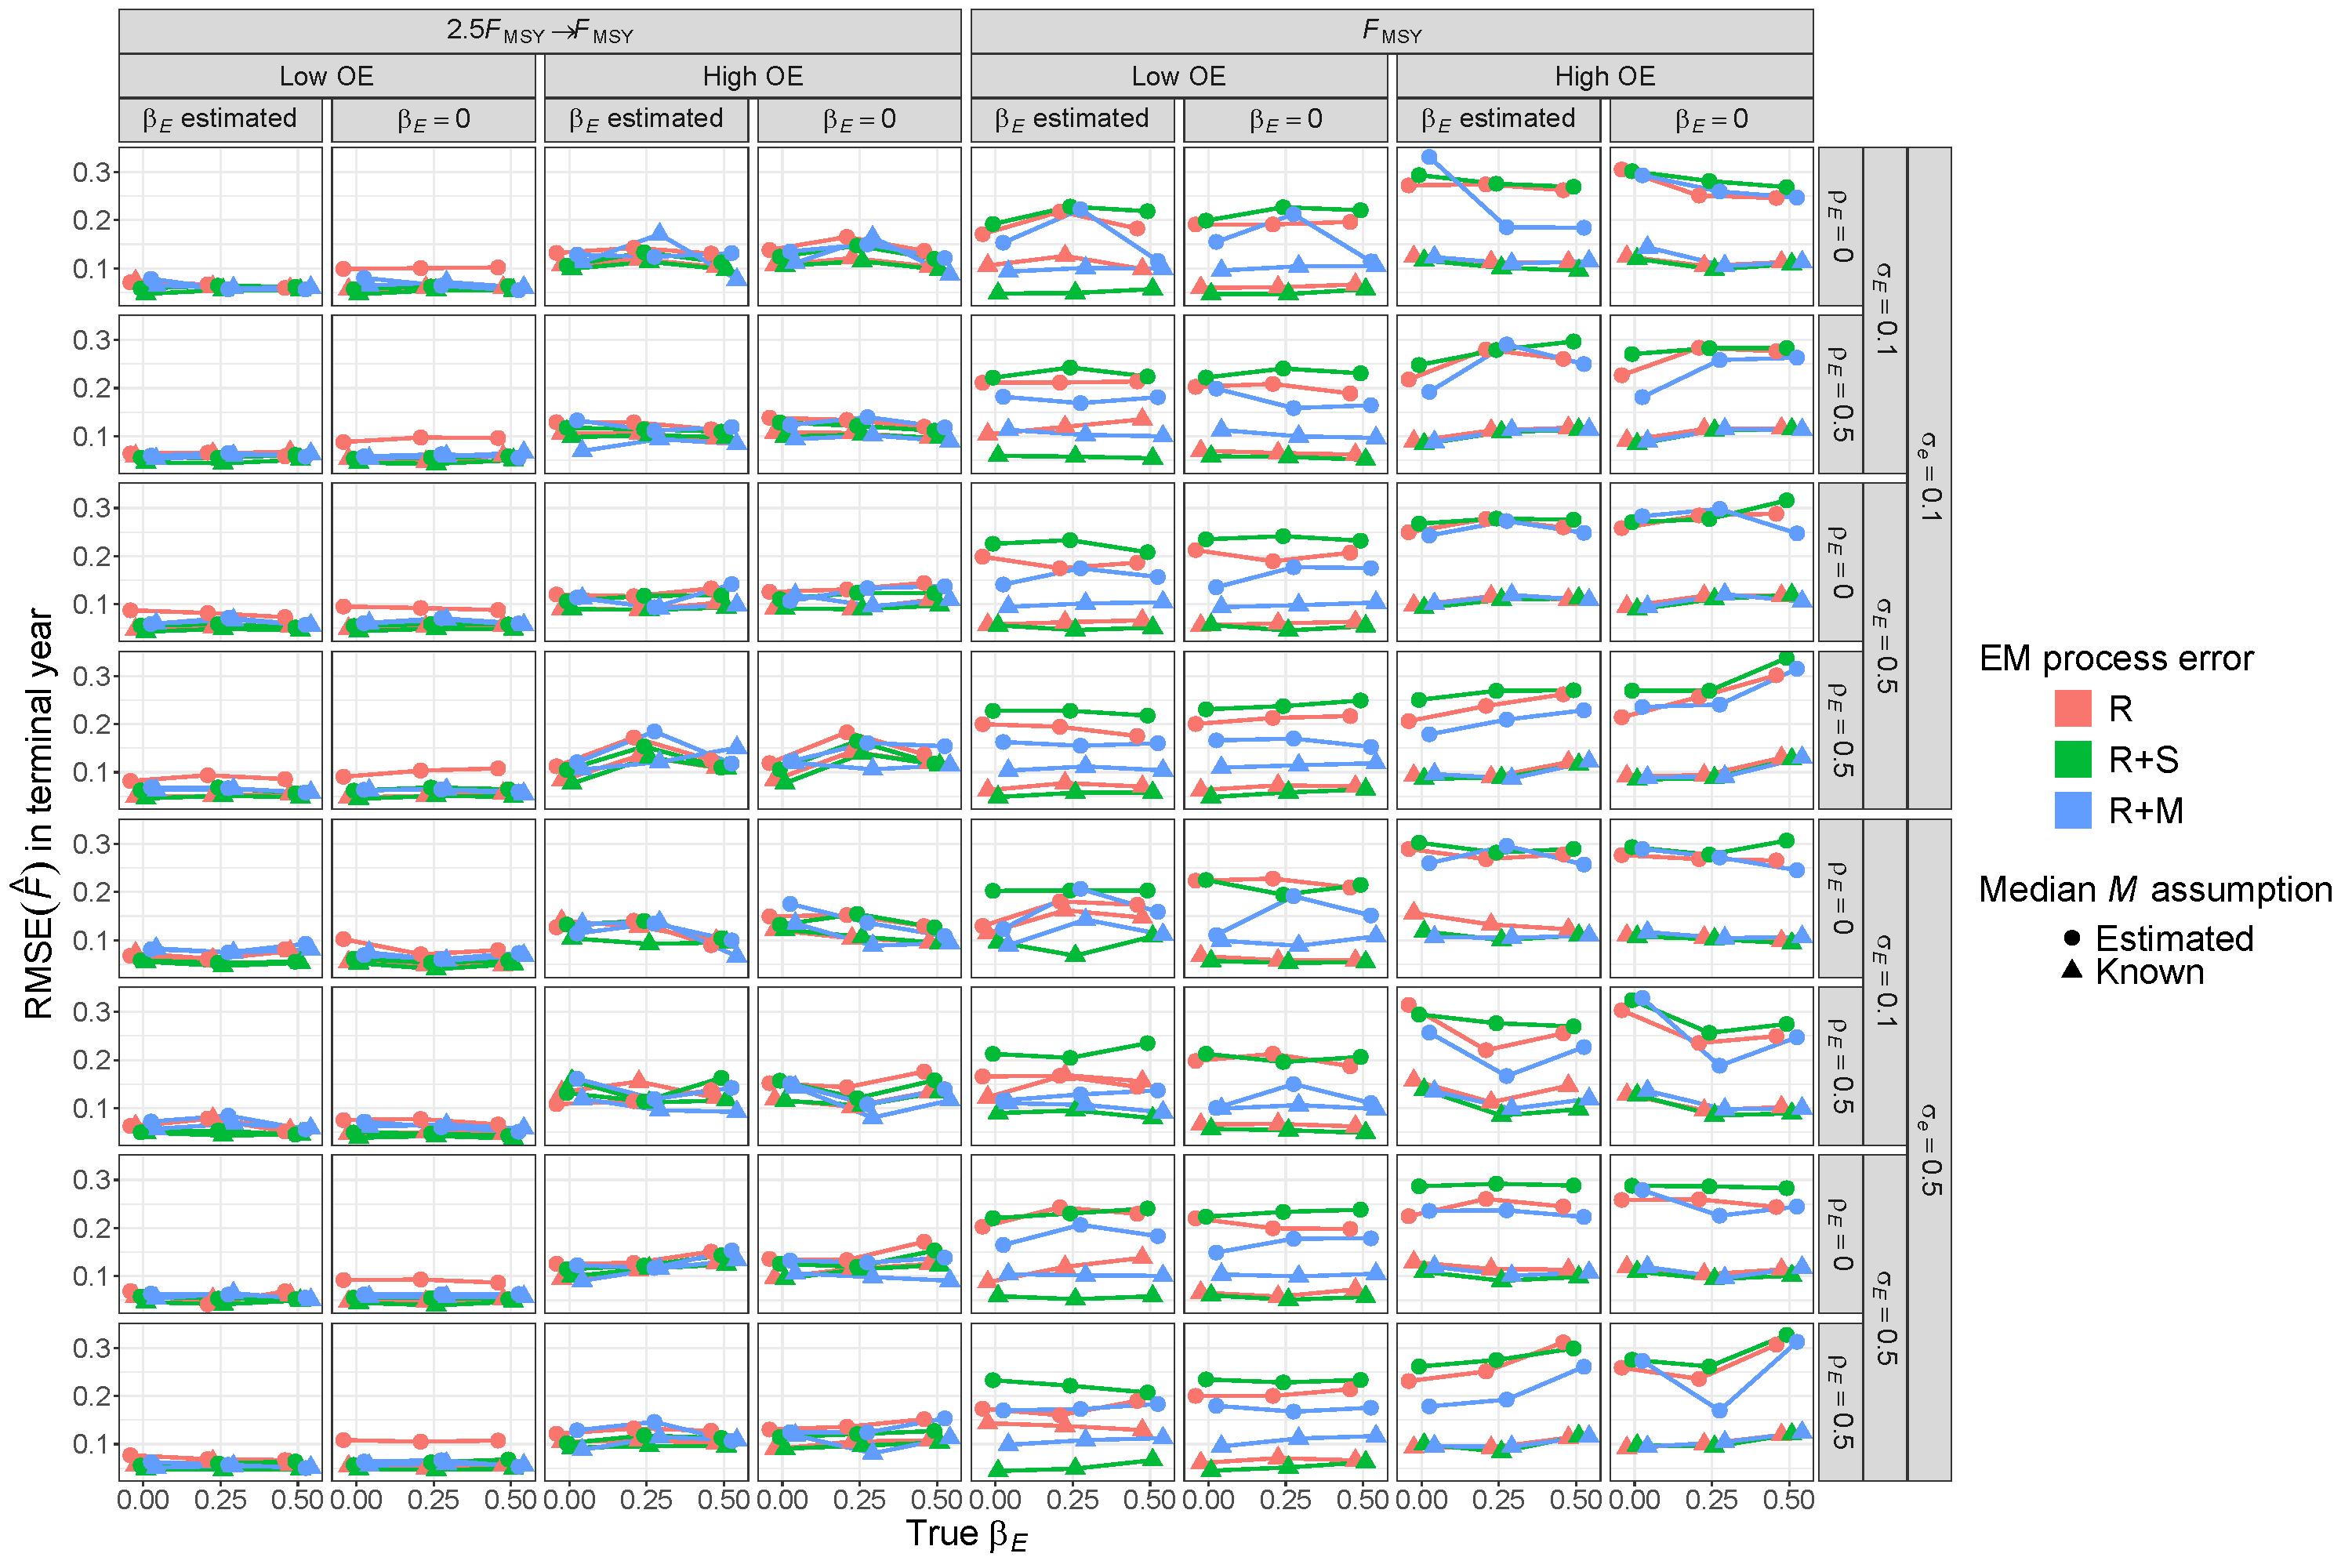
\includegraphics[height = \textheight]{terminal_year_F_rmse_RSom}
\end{center}
\caption{For R+S operating models, RMSE of estimates of fully-selected fishing mortality ($F$)  in the terminal year for estimating models with alternative process error assumptions, treatment of covariate effect ($\beta_E = 0$ or estimated), and treatment of median $M$ parameter ($\beta_M$ estimated or known).}\label{terminal_F_rmse_RSom}
\end{figure}
\end{landscape}

\begin{landscape}
\begin{figure}
\begin{center}
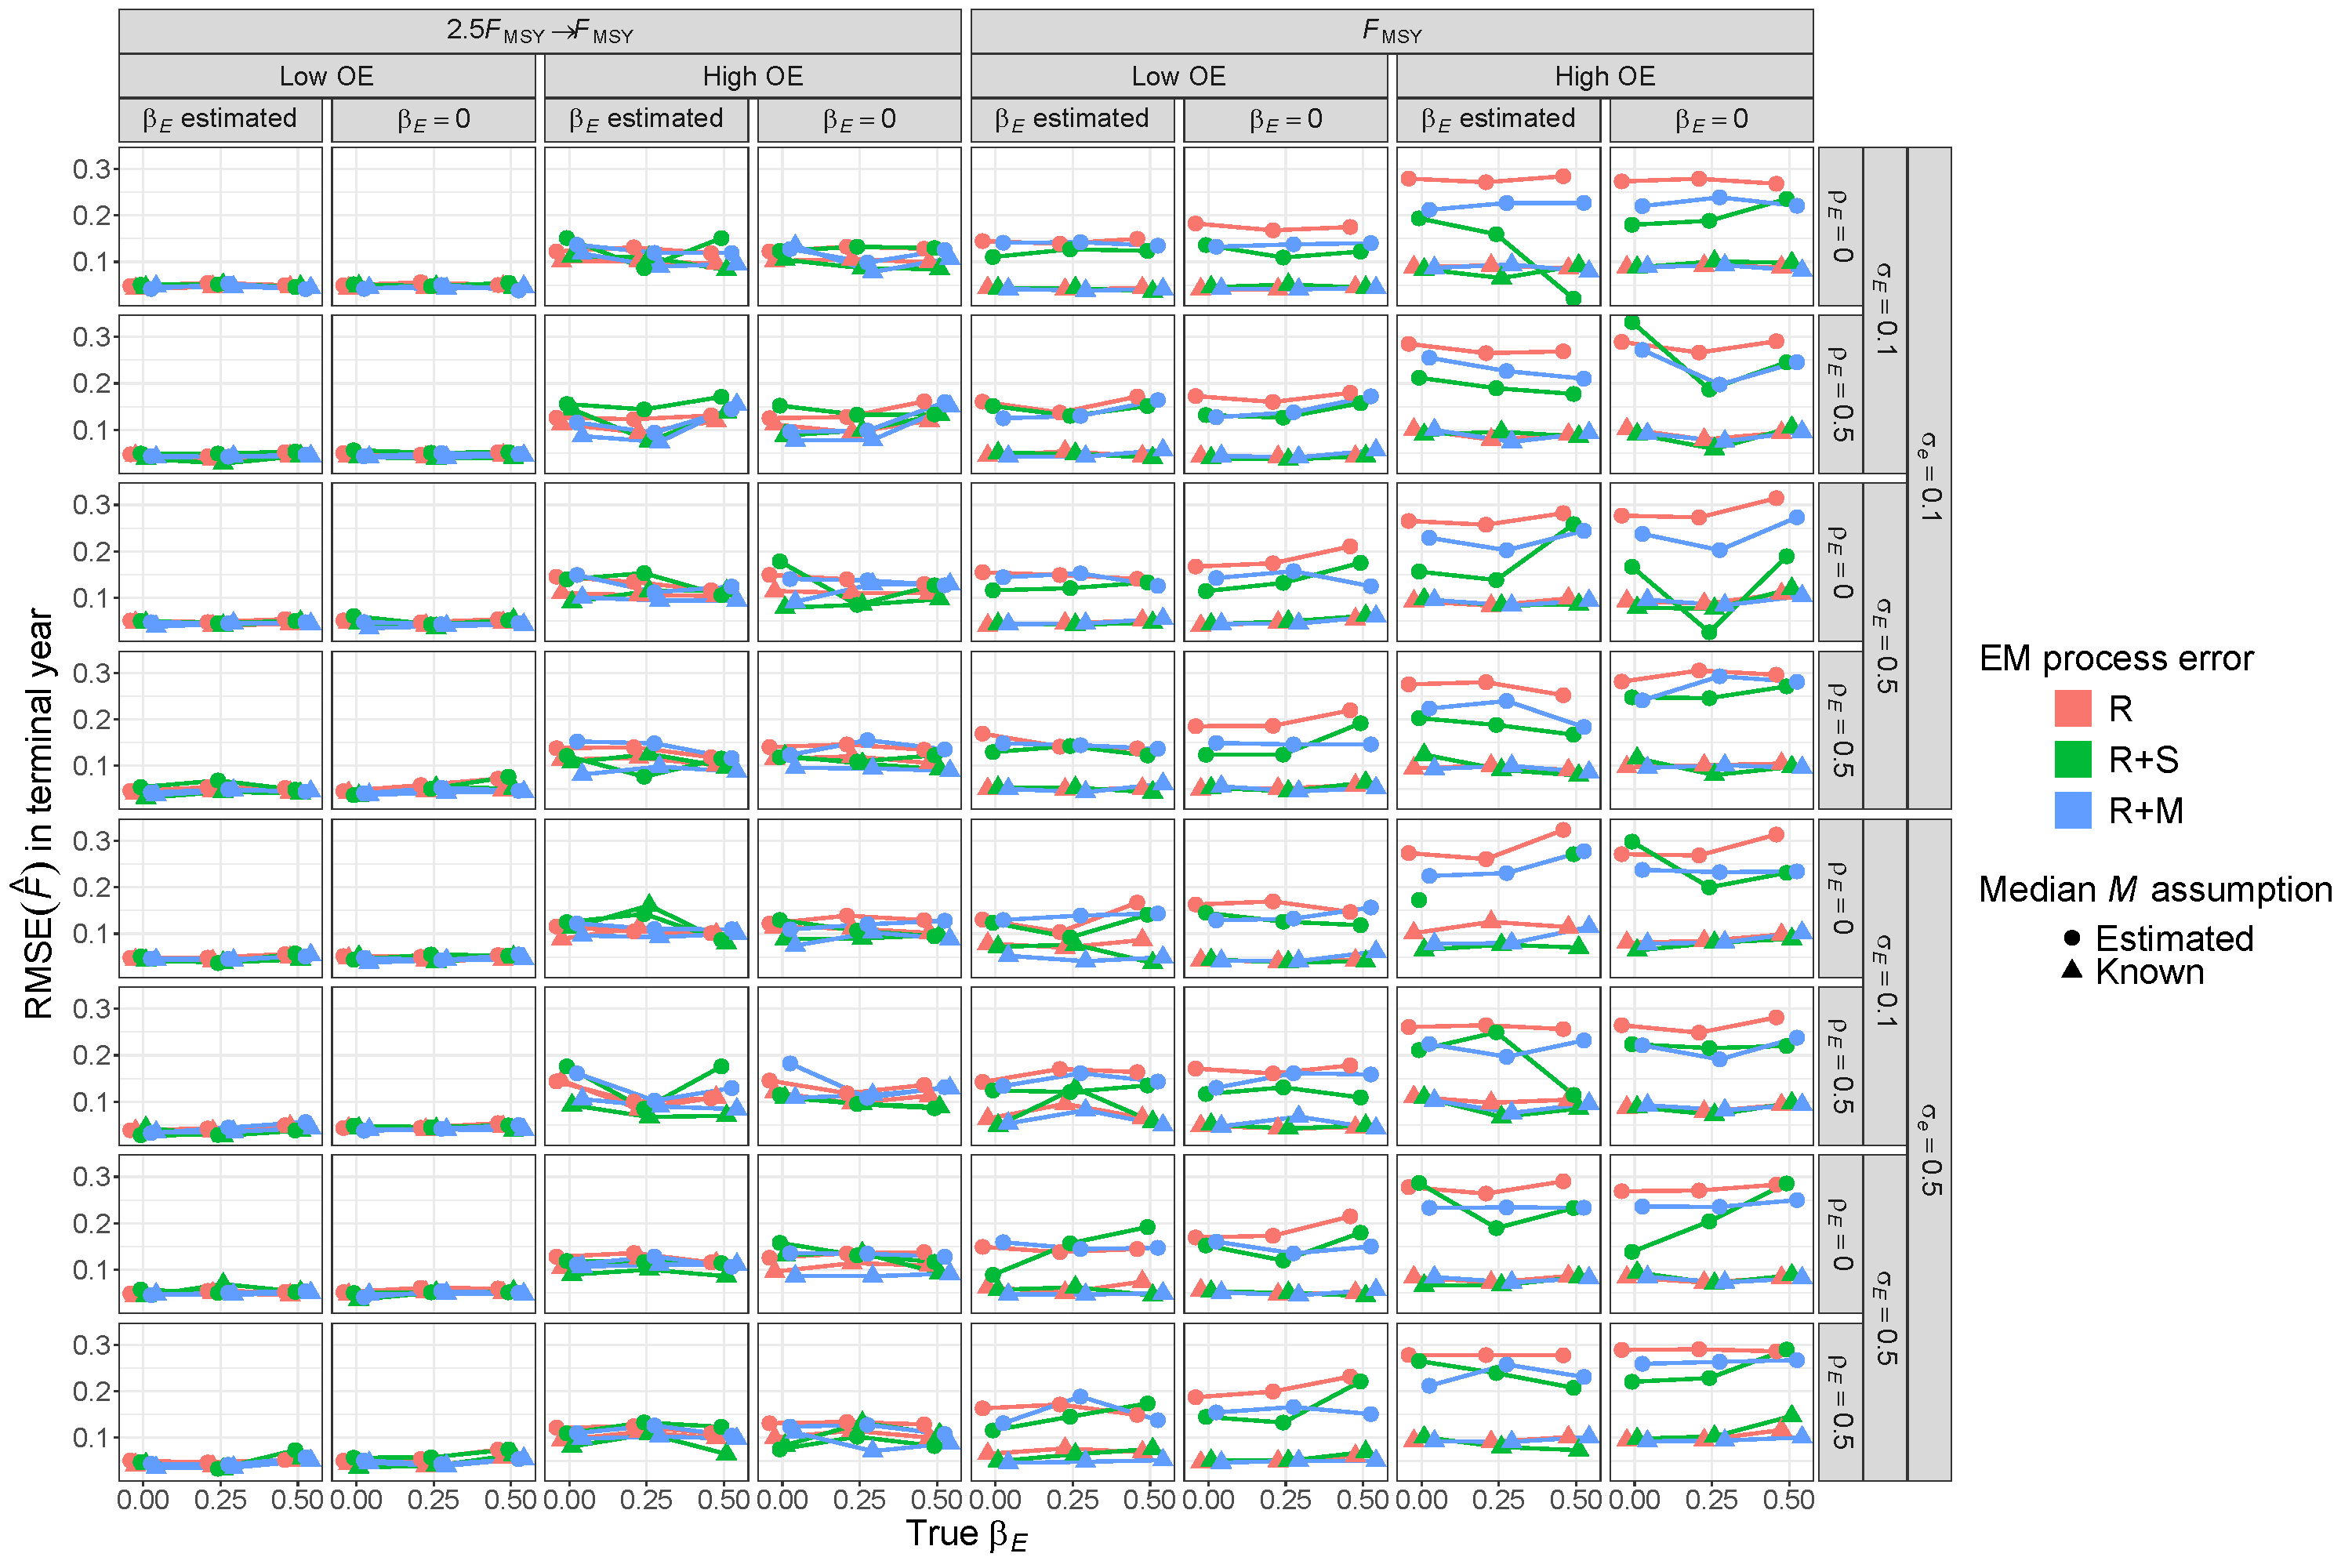
\includegraphics[height = \textheight]{terminal_year_F_rmse_RMom}
\end{center}
\caption{For R+M operating models, RMSE of estimates of fully-selected fishing mortality ($F$)  in the terminal year for estimating models with alternative process error assumptions, treatment of covariate effect ($\beta_E = 0$ or estimated), and treatment of median $M$ parameter ($\beta_M$ estimated or known).}\label{terminal_F_rmse_RMom}
\end{figure}
\end{landscape}

\bibliography{manuscript.bib}

\end{document}
